
\documentclass[notes=show]{beamer}
%\documentclass[handout,xcolor=pdftex,dvipsnames,table]{beamer}

\usepackage{amssymb}
\usepackage{amsmath}
\usepackage{breqn} % Breaks lines
\usepackage[T1]{fontenc}

%\usepackage{mathpazo}
\usepackage{hyperref}
\usepackage{listings}
\usepackage{multimedia}
\usepackage{graphicx}
\usepackage[percent]{overpic}
\usepackage{pgfpages}
\usepackage{pdfpages}
\usepackage{pgfplots}
\usepackage{animate}
\usepackage{mathtools}
\usepackage{threeparttable}
\setbeamertemplate{blocks}[shadow=false]
\usepackage{multirow,dcolumn,booktabs} 
\usepackage{xcolor,colortbl}
\newcommand{\done}{\cellcolor{gray}}  %{0.9}


%% Video stuff
\usepackage{media9}

% Get rid of stupid stuff at the bottom
\beamertemplatenavigationsymbolsempty

% packages for bibs and cites
\usepackage{natbib}
\usepackage{har2nat}
\newcommand{\possessivecite}[1]{\citeauthor{#1}'s \citeyearpar{#1}}
\usepackage{breakcites}
\usepackage{amsmath}
\usepackage{verbatim}
\usepackage{alltt}
\definecolor{myblue}{RGB}{80,80,160}
\definecolor{mygreen}{RGB}{80,160,80}

\DeclareMathOperator{\var}{var} \DeclareMathOperator{\cov}{cov} \DeclareMathOperator{\E}{E} \DeclareMathOperator{\tr}{tr} \DeclareMathOperator{\se}{se} \DeclareMathOperator{\I}{I} \DeclareMathOperator{\sign}{sign} \DeclareMathOperator{\supp}{supp} \DeclareMathOperator{\plim}{plim}
\DeclareMathOperator*{\dlim}{\mathnormal{d}\mkern2mu-lim}
\newcommand\independent{\protect\mathpalette{\protect\independenT}{\perp}}
   \def\independenT#1#2{\mathrel{\rlap{$#1#2$}\mkern2mu{#1#2}}}
\newcommand{\myurlshort}[2]{\href{#1}{\textcolor{gray}{\textsf{#2}}}}
\newcommand*\colvec[1]{\begin{pmatrix}#1\end{pmatrix}}
\setbeamercovered{dynamic}
\usetheme{Warsaw}
\usepackage{tikz}
\usepackage{pgfplots}
\usetikzlibrary{calc, positioning, decorations.pathreplacing, arrows.meta, intersections}
\pgfdeclarelayer{bg}
\pgfdeclarelayer{back}
\pgfdeclarelayer{fg}
\pgfsetlayers{bg,main,fg,back}
\usetikzlibrary{shapes,arrows}

%

\begin{document}

\begin{frame}[plain]

	\begin{center}
	\textbf{Causal Inference and Research Design}  \\  Scott Cunningham (Baylor) 
	\end{center}
	
	\begin{figure}
	\includegraphics[scale=0.5]{./lecture_includes/correlation.png}
	\caption{\myurlshort{http://xkcd.com/552/}{xkcd}}
	\end{figure}

\end{frame}


\title[Causal Inference]{Causal Inference} \subtitle{Applied Econometrics and Research Design}
\author[Cunningham]{Scott Cunningham} \institute[Baylor]{Baylor University}
\date[Spring 2020]{Spring 2020}



%\frame[allowframebreaks]%
%{\frametitle{Table of Contents}\tableofcontents}

\section{Hidden curriculum}

\subsection{Introduction}

\begin{frame}
\begin{center}
\textbf{Where to find this material}
\end{center}

\begin{itemize}
	\item A lot of this material is drawn from my book, \underline{Causal Inference: The Mixtape}, which you can download from my website \url{www.scunning.com} 
%	\item Exercises, datasets and these slides are in the ``Workshop'' Dropbox folder
\end{itemize}
\end{frame}


\begin{frame}[plain]
	\begin{center}
	\textbf{Structure and Assessment}
	\end{center}
	
The fundamental theme linking all lectures will be the estimation of \emph{causal effects}
	\begin{itemize}
	\item Part 1 covers ``the core'' of applied econometrics, including hidden curriculum
	\item Part 2 covers causality foundations like potential outcomes and DAGs
	\item Part 3 covers contemporary research designs
	\end{itemize}

\end{frame}

\begin{frame}[plain]
	\begin{center}
	\textbf{Stata and R}
	\end{center}
	
A secondary goal of the workshop is to provide you with programming examples in Stata and R for implementing some but not all of the procedures we'll cover
	\begin{itemize}
	\item R and Stata code are provided many procedures (with more to come)
	\item I wrote the Stata and had the written by my RAs reviewed by a third exceptional student
	\item Programs and data can be downloaded from my GitHub repository (https://github.com/scunning1975/mixtape)
	\end{itemize}
\end{frame}


\begin{frame}[plain]
	\begin{center}
	\textbf{Textbooks}
	\end{center}
	
Helpful Textbooks imho
		\begin{enumerate}
		\item Cunningham (2018) \myurlshort{http://www.scunning.com} (Mixtape) (under contract with Yale, but I can't share the new version yet -- this deck is the closest thing to it)
		\item Angrist and Pischke (2009) \myurlshort{http://www.amazon.com/Mostly-Harmless-Econometrics-Empiricists-Companion/dp/0691120358/}{Mostly Harmless Econometrics} (MHE)
		\item Morgan and Winship (2014) \myurlshort{http://www.amazon.com/Counterfactuals-Causal-Inference-Principles-Analytical/dp/1107694167//}{Counterfactuals and Causal Inference} (MW)
		\end{enumerate}
\end{frame}

\begin{frame}[plain]
\begin{center}
\textbf{Readings}
\end{center}

Readings: 
		\begin{itemize}
		\item We will also discuss a number of papers in each lecture, each of which you will need to learn inside and out.  
		\item Lecture slides and reading lists are available 
		\item Key literature is contained in the shared dropbox folder which I'll distribute beforehand
		\end{itemize}

\end{frame}



\begin{frame}
\begin{center}
\textbf{About me}
\end{center}

\begin{itemize}
	\item Professor of economics at Baylor (Waco Texas), 
	\item Graduated in 2007 from University of Georgia with a field in econometrics, IO, public, and labor field courses
	\item I knew I was going to be an empiricist, so I made econometrics my main field -- passed field exam on second attempt
	\item Since graduating I've focused on topics in crime and risky sex such as sex work, drug policy, abortion, mental healthcare. 
	\item I knew I couldn't achieve my goals without learning causal inference which I could tell I had only a vague understanding of
	\item This is because causal inference isn't taught historically in traditional econometrics 
\end{itemize}

\end{frame}





\begin{frame}[plain]
\begin{center}
\textbf{Sad story (to me!)}
\end{center}

\begin{itemize}
\item Once upon a time there was a boy who wrote a job market paper using the NLSY97. 
\item This boy presented the findings a half dozen times, spoke to the media a few times, got 17 interviews at the ASSA, 7 flyouts, and an offer from Baylor
\item He submitted the job market paper to the \emph{Journal of Human Resources}, a top field journal in labor, and received a ``revise and resubmit'' request from the editor (woo hoo!)
\end{itemize}

\end{frame}

\begin{frame}[plain]
\begin{center}
\textbf{The horror!}
\end{center}

\begin{itemize}
\item But then digging into his one directory, he found countless versions of his do file and hundreds of files with random names
\item And once he finally was able to get the code running again, he found a critical coding error that when corrected (``destroyed'') his results
\item The young boy was devastated and never resubmitted which he does not recommend (but he was sad!)
\end{itemize}

\end{frame}

\subsection{Workflow workflow workflow}

\begin{frame}
\begin{center}
\textbf{All competent empirical work is a mousetrap}
\end{center}

``Happy families are all alike; every unhappy family is unhappy in its own way.'' - Leo Tolstoy, \underline{Anna Karenina}
\bigskip

``Good empirical work is all alike; every bad empirical work is bad in its own way.'' - Scott Cunningham, \underline{This slide}

\end{frame}


\begin{frame}[plain]
\begin{center}
\textbf{Cunningham Empirical Workflow Conjecture}
\end{center}

\begin{itemize}
\item The cause of most of your errors is \textbf{not} due to insufficient knowledge of syntax in your chosen programming language
\item The cause of most of your errors is due to a poorly designed empirical workflow
\end{itemize}

\end{frame}

\begin{frame}[plain]
\begin{center}
\textbf{Workflow}
\end{center}

Wikipedia definition: 

\begin{quote}
``A workflow consists of an orchestrated and repeatable pattern of activity, enabled by the systematic organization of resources into processes that transform materials, provide services, or process information.''
\end{quote}

Dictionary definition:
\begin{quote}
``the sequence of industrial, administrative, or other processes through which a piece of work passes from initiation to completion.''
\end{quote}

\end{frame}



\begin{frame}[plain]
\begin{center}
\textbf{Empirical workflow}
\end{center}

\begin{itemize}
\item Workflow is a fixed set of routines you bind yourself to which when followed identifies the most common errors
	\begin{itemize}
	\item Think of it as your morning routine: alarm goes off, go to wash up, make your coffee, check Twitter, repeat \emph{ad infinitum}
	\end{itemize}
\item Finding the outlier errors is a different task;  empirical workflows catch typical and common errors created by the modal data generating processes
\end{itemize}

\end{frame}


\begin{frame}[plain]
\begin{center}
\textbf{Why do we use checklists?}
\end{center}

\begin{itemize}
\item Before going on a trip, you use a checklist to make sure you have everything you need
	\begin{itemize}
	\item Charger (check), underwear (check), toothbrush (check), passport (oops), \dots
	\end{itemize}
\item The empirical checklist is solely referring to the intermediate step between ``getting the data'' and ``analyzing the data''
\item It largely focuses on ensuring data quality for the most common, easiest to identify, situations you'll find yourself in
\end{itemize}

\end{frame}


\begin{frame}[plain]
\begin{center}
\textbf{Simple checks}
\end{center}

\begin{itemize}
\item Your checklist should be a few simple, yet non-negotiable, programming commands and exercises to check for coding errors
\item Let's discuss a few
\end{itemize}

\end{frame}


\begin{frame}[plain]
\begin{center}
\textbf{Time}
\end{center}

\begin{itemize}
\item People often think empirical research is about ``getting the data'' and ``analyzing the data''
\item They have an ``off to the races'' mindset
\item Just like running a marathon involves far far more time training than you ever spend running the marathon, doing empirical research involves far far more time doing tedious, repetitive tasks
\item Since you do the tedious tasks repeatedly, they have the \emph{most} potential for error which can be catastrophic
\item How can we minimize these errors through a checklist?
\end{itemize}

\end{frame}

\begin{frame}[plain]

\begin{figure}
\includegraphics[scale=0.1]{./lecture_includes/time.png}
\caption{Image from Wenfei Xu at Columbia}
\end{figure}

\end{frame}

\begin{frame}[plain]
\begin{center}
\textbf{Read the codebook}
\end{center}

\begin{itemize}
\item We stand on the shoulders of giants
\item Few like reading the codebook as it is not gripping literature 
\item But the codebook explains how to interpret the data you have acquired and it is not a step you can skip
\item Set aside time to study it, and have it in a place where you can regularly return to it
\item This goes for the \texttt{readme} that accompanies some datasets, too. 
\end{itemize}

\end{frame}

\begin{frame}[plain]
\begin{center}
\textbf{Look at the data}
\end{center}

\begin{itemize}
\item The eyeball is not nearly appreciated enough for its ability to spot problems
\item Use \texttt{browse} or excel to just read the spreadsheet with your eyes.
\item Scroll through the variables and accompany yourself with what you've got visually
\end{itemize}

\end{frame}


\begin{frame}[plain]

\begin{figure}
\centering
\includegraphics[scale=0.15]{./lecture_includes/browse.png}
\end{figure}

\end{frame}


\begin{frame}[plain]

\begin{figure}
\centering
\includegraphics[scale=0.10]{./lecture_includes/burglaries.jpg}
\end{figure}

\end{frame}





\begin{frame}[plain]
\begin{center}
\textbf{Missing observations}
\end{center}

\begin{itemize}
\item Check the size of your dataset in Stata using \texttt{count}
\item Check the number of observations per variable in Stata using \texttt{summarize}
	\begin{itemize}
	\item String variables will always report zero observations under \texttt{summarize} so \texttt{count if X==""} will work
	\end{itemize}
\item Use \texttt{tabulate} also because oftentimes missing observations are recorded with a $-9$ or some other illogical negative value
\end{itemize}

\end{frame}

\begin{frame}[plain]
\begin{center}
\textbf{Missing years}
\end{center}

\begin{itemize}
\item Panel data can be overwhelming bc looking at each state/city/firm/county borders on the impossible
\item Start with \texttt{collapse} to the national level by year and simply \texttt{list} to see if anything looks strange
	\begin{itemize}
	\item What's ``strange'' look like?
	\item Well wouldn't it be strange if national unemployment rates were zero in any year?
	\end{itemize}
\item You can use \texttt{xtline} to see time series for panel identifiers, with or without the subcommand of \texttt{overlay}
\end{itemize}

\end{frame}


\begin{frame}[plain]

\begin{figure}
\centering
\includegraphics[scale=0.25]{./lecture_includes/collapse.png}
\end{figure}

\end{frame}



\begin{frame}[plain]

\begin{figure}
\centering
\includegraphics[scale=0.1]{./lecture_includes/panel_calories.png}
\end{figure}

\end{frame}

\begin{frame}[plain]

\begin{figure}
\centering
\includegraphics[scale=0.1]{./lecture_includes/panel_calories_b.png}
\end{figure}

\end{frame}

\begin{frame}[plain]
\begin{center}
\textbf{Panel observations are $N \times T$}
\end{center}

\begin{itemize}
\item Say you have 51 state units (50 states plus DC) and 10 years
\item $51 \times 10 = 510$ observations
\item If you do not have 510 observations, then you have an unbalanced panel; if you have 510 observations you have a balanced panel
\item Check the patterns using \texttt{xtdescribe} and simple counting tricks
\end{itemize}

\end{frame}


\begin{frame}[plain]

\begin{figure}
\centering
\includegraphics[scale=0.1]{./lecture_includes/unbalanced_panel.png}
\end{figure}

\end{frame}


\begin{frame}[plain]

\begin{figure}
\centering
\includegraphics[scale=0.2]{./lecture_includes/unbalanced_panel_b.png}
\end{figure}

\end{frame}


\begin{frame}[plain]
\begin{center}
\textbf{Merge}
\end{center}

\begin{itemize}
\item During a stage of arranging datasets, you will likely merge -- oftentimes a lot
\item Make sure you count before and after you merge so you can figure out what went wrong, if anything
\item Also make sure you're using the contemporary m:m syntax as many an excellent empiricists have been hurt by merge syntax errors
\end{itemize}

\end{frame}


\begin{frame}[plain]

\begin{figure}
\centering
\includegraphics[scale=0.2]{./lecture_includes/merge.png}
\end{figure}

\end{frame}


\begin{frame}[plain]
\begin{center}
\textbf{Don't forget the question}
\end{center}


\begin{itemize}
\item ``Exploring the data'' is intoxicating to the point of distracting
\item ``All you can do is write the best paper on the question you're studying'' -- Mark Hoekstra
	\begin{itemize}
	\item Note he didn't say ``Write the best paper you're capable of writing''
	\item He said \textbf{the best paper}
	\item Important therefore to choose the right questions with real upside
	\end{itemize}
\item Slow down, think big picture, force yourself to figure out exactly what your question is, who is in your sample (and importantly who won't be) and what time periods you'll pull
\end{itemize}

\end{frame}


\subsection{Directories}


\begin{frame}
\begin{center}
\textbf{Organize your directories}
\end{center}

\begin{itemize}
\item After the coding error fiasco, I spent a lot of time wondering how this could happen
\item I decided it was partly because of four problems related to
	\begin{enumerate}
	\item organized subdirectories
	\item automation
	\item naming conventions
	\item version control
	\end{enumerate}
\item I'll discuss each but I highly recommend that you just read Gentzkow and Shapiro's excellent resource ``Code and Data for the Social Sciences: A Practitioner's Guide'' \url{https://web.stanford.edu/~gentzkow/research/CodeAndData.pdf}
\end{itemize}

\end{frame}


\begin{frame}[plain]
\begin{center}
\textbf{No correct organization}
\end{center}

\begin{itemize}
\item There is no correct way to organize your directories, 
\item But all competent empiricists have adopted an intentional philosophy of how to organize their directories
\item Why? Because you're writing for your future self, and your future self is lazy, distracted, disinterested and busy
\end{itemize}

\end{frame}




\begin{frame}
\begin{center}
\textbf{Directories}
\end{center}

\begin{itemize}
\item The typical applied micro project may have hundreds of files of various type and will take \emph{years} just to finish not including time to publication
\item So simply finding the files you need becomes more difficult if everything is stored in the same place
\item When I start a new project, the first thing I do is create the following directories
\end{itemize}

\end{frame}


\begin{frame}[plain]
\begin{center}
\textbf{Subdirectory organization}
\end{center}


\begin{figure}

\includegraphics{./lecture_includes/directories.png}
\end{figure}

1) Name the project (``Texas'')

\end{frame}

\begin{frame}[plain]
\begin{center}
\textbf{Subdirectory organization}
\end{center}

\begin{figure}
\includegraphics[scale=0.5]{./lecture_includes/articles.png}
\end{figure}

2) A subdirectory for all articles you cite in the paper

\end{frame}

\begin{frame}[plain]
\begin{center}
\textbf{Subdirectory organization}
\end{center}

\begin{figure}
\includegraphics[scale=0.5]{./lecture_includes/data.png}
\end{figure}

3) Data subdirectory containing all datasets

\end{frame}

\begin{frame}[plain]
\begin{center}
\textbf{Subdirectory organization}
\end{center}

\begin{figure}
\includegraphics[scale=0.5]{./lecture_includes/do.png}
\end{figure}

4) A subdirectory for all do files and log files
\end{frame}

\begin{frame}[plain]
\begin{center}
\textbf{Subdirectory organization}
\end{center}

\begin{figure}
\includegraphics[scale=0.5]{./lecture_includes/figures.png}
\end{figure}

5) All figures produced by Stata or image files
\end{frame}


\begin{frame}[plain]
\begin{center}
\textbf{Subdirectory organization}
\end{center}

\begin{figure}
\includegraphics[scale=0.5]{./lecture_includes/misc.png}
\end{figure}

6) Project-specific heterogeneity (e.g., ``Inference'', ``Grants'', ``Interview notes'', ``Presentations'', ``Misc'') 
\end{frame}

\begin{frame}[plain]
\begin{center}
\textbf{Subdirectory organization}
\end{center}

\begin{figure}
\includegraphics[scale=0.5]{./lecture_includes/tables.png}
\end{figure}

7) All tables generated by Stata (e.g., .tex tables produced by -estout-)
\end{frame}

\begin{frame}[plain]
\begin{center}
\textbf{Subdirectory organization}
\end{center}

\begin{figure}
\includegraphics[scale=0.5]{./lecture_includes/writing.png}
\end{figure}

8) A subdirectory reserved only for writing
\end{frame}


\subsection{Do files and R programs}

\begin{frame}
\begin{center}
\textbf{Always use scripting programs NOT GUI}
\end{center}

\begin{itemize}
\item Guess what - your future self doesn't even remember making do files, tables or figures, let alone typing into GUI command line
\item Therefore throw her a bone, hold her hand and walk her exactly through everything
\item Which means you've got to have replicable scripting files*
	\begin{itemize}
	\item * Sure, sometimes use the the command line for messing around
	\item But then put that messing around in the program
	\end{itemize}
\end{itemize}

\end{frame}

\begin{frame}[plain]
\begin{center}
\textbf{Good text editor}
\end{center}

\begin{itemize}
\item Remember: the goal is to make beautiful programs
\item Invest in a good text editor which has bundling capabilities that will integrate with Stata, R or LaTeX
\item I use Textmate 2 because I use a Mac and in addition to a Stata and R bundle, it also allows for \emph{column} editing
\item PC users tend to love Sublime for the same reasons
\item Stata and Rstudio also come with built-in text editors, which use slick colors for various types of programming commands
\end{itemize}

\end{frame}

\begin{frame}[plain]
\begin{center}
\textbf{Headers}
\end{center}

\begin{figure}
\includegraphics[scale=0.35]{./lecture_includes/headers.png}
\end{figure}

\end{frame}

\begin{frame}[plain]
\begin{center}
\textbf{Speak clearly}
\end{center}

``Be conservative in what you do; be liberal in what you accept from others.'' - Jon Postel 
\bigskip

\begin{itemize}
\item Smart sounding quote about both programming and relationships
\item Your future self is time constrained, so explain \emph{everything} to her as well as write clear code
\item Optimally document your programs
\item But speak your future self's love language so she understands
\end{itemize}

\end{frame}


\begin{frame}[plain]
\begin{center}
\textbf{Automating Tables and Figures}
\end{center}

\begin{itemize}
\item Your goal is to make ``beautiful tables'' that are never edited post-production as well as readable on their own
\item Large fixed costs learning commands like -estout- or -outreg2-: incur them bc marginal costs are zero
\item I use -estout- because Jann has written an excellent help file at \url{http://repec.org/bocode/e/estout/hlp_esttab.html} but many like -outreg2- 
\item Learn -twoway- and/or -ggplot2- and make ``beautiful pictures'' too
\end{itemize}
\end{frame}



\subsection{Naming conventions}

\begin{frame}
\begin{center}
\textbf{Different elements}
\end{center}

\begin{itemize}
\item When I found my error, and after I regained my exposure, I eventually developed a system of naming
	\begin{enumerate}
	\item  variables, 
	\item datasets, and 
	\item do files
	\end{enumerate}
\item As these are the three things you repeatedly use, you need to have a system, even if not mine
\end{itemize}

\end{frame}

\begin{frame}[plain]
\begin{center}
\textbf{Naming conventions for variables}
\end{center}

\begin{itemize}
\item Variables should be readable to a stranger
	\begin{itemize}
	\item Say that you want to create the product of two variables. Name it the two variables with an underscore
	\item \texttt{gen price_mpg = price * mpg}
	\end{itemize}
\item Otherwise name the variable exactly what it is
	\begin{itemize}
	\item gen bmi = weight / (height^2 * 703)
	\end{itemize}
\item Avoid meaningless words (e.g., \texttt{lmb2}), dating (e.g., \texttt{temp05012020}) and numbering (e.g., \texttt{outcome25}) as your future self will be confused
\end{itemize}

\end{frame}

\begin{frame}[plain]
\begin{center}
\textbf{Naming datasets and do files}
\end{center}

\begin{itemize}

\item The overarching goal is always to name things so that a stranger seeing them can know what they are
\item One day you will be the stranger on your own project!  Make it easy on your future self!
\item Choose some combination of simplicity and clarity but whatever you do, be consistent
\item Avoid numbering datasets unless the numbers correspond to some meaningful thing, like randomization inference where each file is a set of coefficients and numbered according to FIPS index

\end{itemize}

\end{frame}

\begin{frame}[plain]
\begin{center}
\textbf{Version control}
\end{center}

\begin{itemize}
	\item People swear by git, particularly Gentzkow and Shapiro
	\item I use Dropbox, and have for years. They have some version history for instance, though I'm not sure if it compares to git's capabilities.
	\item I'm slowly learning git and use git Tower, but many use the command line in Terminal
	\item Ideally your system allows you to revert to earlier versions without having ten billion files with names like \texttt{prison\_03102019_sc.do}, etc. 
\end{itemize}

\end{frame}

\subsection{Soft skills}

\begin{frame}
\begin{center}
\textbf{Selling your work}
\end{center}

\begin{itemize}
\item If you don't advocate for your work, \emph{no one will}. 
\item Network, network, network
\item You will need to become an expert in 1.5 areas, and you will need experts in those 1.5 areas to agree
\item Study the effective of rhetoric of successful economists who expertly communicate their work to others both in their writing of the actual manuscript, as well as the presentation and promotion of their work
\end{itemize}

\end{frame}

\begin{frame}[plain]
\begin{center}
\textbf{Find your mentors and sponsors}
\end{center}

\begin{itemize}
\item Working with senior people at some point becomes necessary
\item Good news: many senior people want to help you
\item Bad news: they don't know who you are and can't find you
\item It's a two sided matching problem
\item Introduce yourself in socially appropriate ways!
\end{itemize}

\end{frame}

\begin{frame}[plain]
\begin{center}
\textbf{Al Roth story}
\end{center}

\begin{itemize}
\item I wrote Al Roth in 2007 and like Robert Browning to Elizabeth Barrett introduced myself by saying ``I love your book on twosided matching with Sotomayor with all my heart.''
\item We became pen pals and then he won the Nobel Prize
\item Scared, I wrote to congratulate him on the day he won and he immediately asked to help me 
\item ``Interpersonal favors are meant to be paid forward not backwards'' - Roth to me after a \emph{second} favor!
\item Nobody can help you if you don't know them bc help, sponsorship and mentoring is a two sided matching problem
\end{itemize}

\end{frame}


\begin{frame}[plain]
\begin{center}
\textbf{More readings}
\end{center}

\begin{itemize}
\item I've put several deck of slides and helpful articles for you in the dropbox folder
\item Jesse Shapiro's ``How to Present an Applied Micro Paper''
\item Gentzkow and Shapiro's coding practices manual
\item Rachael Meager on presenting as an academic
\item Ljubica ``LJ'' Ristovska's language agnostic guide to programming for economists
\item Grant McDermott on Version Control using Github \url{https://raw.githack.com/uo-ec607/lectures/master/02-git/02-Git.html\#1}

\end{itemize}

\end{frame}

\begin{frame}[plain]
\begin{center}
\textbf{Data Visualization}
\end{center}

Every project should present compelling graphics summarizing the main results and main takeaway
\begin{itemize}
\item Study other people's pictures and get help from experts
	\begin{enumerate}
	\item Kieran Healy's 2018 \underline{Visualization: A Practical Introduction} (Princeton University Press); free version is \url{http://socviz.co/index.html\#preface}. 
	\item Ed Tufte's book \underline{Visual display of quantitative information} is classic, but more a coffee table book plus no programming assistance. 
	\end{enumerate}
\item Learn Stata's -twoway- capabilities and/or R's -ggplot2-
\end{itemize}

\end{frame}

\section{Foundational causality stuff}

\subsection{Regression review}

\begin{frame}
\begin{center}
\textbf{Introduction: OLS Review}
\end{center}

\begin{itemize}
\item Derivation of the OLS estimator
\item Algebraic properties of OLS
\item Statistical Properties of OLS
\item Variance of OLS and standard errors
\end{itemize}

\end{frame}

\begin{frame}[plain]
	\begin{center}
	\textbf{Foundations of scientific knowledge}
	\end{center}
 
Scientific methodologies are the epistemological foundation of scientific knowledge
			\begin{itemize}
		    	\item Science does not collect evidence in order to ``prove'' what people already believe or want others to believe
			\item Science accepts unexpected and even undesirable answers
			\item Science is process oriented, not outcome oriented
			\end{itemize}

\end{frame}


\begin{frame}[plain]
 \begin{center}
  Terminology \linebreak
  \begin{tabular}{|c|c|}
  \hline
  $y$ & $x$ \\ \hline
  Dependent Variable & Independent Variable \\ \hline
  Explained Variable & Explanatory Variable \\ \hline
  Response Variable & Control Variable \\ \hline
  Predicted Variable & Predictor Variable \\ \hline
  Regressand & Regressor \\ \hline
  LHS & RHS \\ \hline
  \end{tabular}
 \end{center}

 The terms ``explained'' and ``explanatory'' are probably best, as they are the most descriptive and widely applicable. But ``dependent'' and ``independent'' are used often. (The ``independence'' here is not really statistical independence.)
\end{frame}

\begin{frame}[plain]
 We said we must confront three issues:
 
 \begin{enumerate}
  \item How do we allow factors other than $x$ to affect $y$?

  \item What is the functional relationship between $y$ and $x$?

  \item How can we be sure we are capturing a ceteris paribus relationship between $y$ and $x$?
 \end{enumerate}
 
 We will argue that the simple regression model

 \begin{equation}
  y=\beta _{0}+\beta _{1}x+u
 \end{equation}
 addresses each of them.
\end{frame}

\begin{frame}[plain]
\begin{center}
\textbf{Simple linear regression model}
\end{center}

\begin{itemize}
\item The simple linear regression (SLR) model is a population model. 
\item When it comes to \emph{estimating} $\beta _{1}$ (and $\beta _{0}$) using a random sample of data, we must restrict how $u$ and $x$ are related to each other.
\item What we must do is restrict the way $u$ and $x$ relate to each other in the population.
\end{itemize}
\end{frame}

\begin{frame}[plain]
\begin{center}
\textbf{The error term}
\end{center}

We make a simplifying assumption (without loss of generality): the average, or expected, value of $u$ is zero in the population:

 \begin{equation}
  E(u)=0
 \end{equation}
 where $E(\cdot )$ is the expected value operator.

\end{frame}

\begin{frame}[plain]
\begin{center}
\textbf{The intercept}
\end{center}
 The presence of $\beta _{0}$ in \begin{equation}
  y=\beta _{0}+\beta _{1}x+u
 \end{equation}
 
 allows us to assume $E(u)=0$. If the average of $u$ is different from zero, say $\alpha _{0}$, we just adjust the intercept, leaving the slope the same:\begin{equation}
  y=(\beta _{0}+\alpha _{0})+\beta _{1}x+(u-\alpha _{0})
 \end{equation}
 
 where $\alpha _{0}=E(u)$. The new error is $u-\alpha _{0}$ and the new intercept is $\beta _{0}+\alpha _{0}$. The important point is that the slope, $\beta _{1}$, has not changed.

\end{frame}

\begin{frame}[plain]
\begin{center}
\textbf{Mean independence of the error term}
\end{center}


 An assumption that meshes well with our introductory treatment involves the mean of the error term for each ``slice'' of the population determined by values of $x$:

 \begin{equation}
  E(u|x)=E(u)\text{, all values }x
 \end{equation}
 where $E(u|x)$ means ``the expected value of $u$ given $x$''.

 Then, we say $u$ is \textbf{mean independent} of $x$.

\end{frame}

\begin{frame}[plain]
\begin{center}
\textbf{Distribution of ability across education}
\end{center}


\begin{itemize}
 
  \item Suppose $u$ is ``ability'' and $x$ is years of education. We need, for example,

   \begin{equation*}
    E(ability|x=8)=E(ability|x=12)=E(ability|x=16)
   \end{equation*}
  so that the average ability is the same in the different portions of the population with an 8$^{th}$ grade education, a 12$^{th}$ grade education, and a four-year college education.

  \item Because people choose education levels partly based on ability, this assumption is almost certainly false.
 
 \end{itemize}
 
\end{frame}

\begin{frame}[plain]
\begin{center}
\textbf{Zero conditional mean assumption}
\end{center}

 Combining $E(u|x)=E(u)$ (the substantive assumption) with $E(u)=0$ (a normalization) gives the \textbf{zero conditional mean assumption}.

 \begin{equation}
  E(u|x)=0\text{, all values }x
 \end{equation}

\end{frame}

\begin{frame}[plain]
\begin{center}
\textbf{Population regression function}
\end{center}
Because the conditional expected value is a linear operator, $E(u|x)=0$ implies

  \begin{equation}
   E(y|x)=\beta _{0}+\beta _{1}x
  \end{equation}
 which shows the \textbf{population regression function} is a linear function of $x$.

\end{frame}


\begin{frame}[plain]

\begin{itemize}
  \item The straight line in the graph on the next page is what Wooldridge calls the \textbf{population regression function}, and what Angrist and Pischke call the \textbf{conditional expectation function}$$E(y|x)=\beta _{0}+\beta _{1}x$$
  \item The conditional distribution of $y$ at three different values of $x$ are superimposed. for a given value of $x$, we see a range of $y$ values: remember, $y=\beta_{0}+\beta _{1}x+u$, and $u$ has a distribution in the population.
\end{itemize}

\end{frame}

\begin{frame}[plain]

\begin{figure}
\includegraphics[scale=0.7]{./lecture_includes/wooldridge_fig21.pdf}
\end{figure}
\end{frame}

\subsubsection{Deriving the Ordinary Least Squares Estimates}

\begin{frame}[plain]

 \begin{center}
  \textbf{Deriving the Ordinary Least Squares Estimates}
 \end{center}
 \begin{itemize}
  \item Given data on $x$ and $y$, how can we estimate the population parameters, $\beta _{0}$ and $\beta _{1}$?

  \item Let $\{(x_{i},y_{i}):i=1,2,...,n\}$ be a \textbf{random} sample of size $n$ (the number of observations) from the population.
  \item Plug any observation into the population equation:
   \begin{equation}
    y_{i}=\beta _{0}+\beta _{1}x_{i}+u_{i}
   \end{equation}
    where the $i$ subscript indicates a particular observation.
  \item We observe $y_{i}$ and $x_{i}$, but not $u_{i}$ (but we know it is there).
 \end{itemize}
\end{frame}

\begin{frame}[plain]
We use the two population restrictions:

 \begin{eqnarray*}
  E(u)=0 \\
  Cov(x,u)=0
 \end{eqnarray*}
to obtain estimating equations for $\beta _{0}$ and $\beta _{1}$. We talked about the first condition. The second condition means that $x$ and $u$ are uncorrelated. Both conditions are implied by $E(u|x)=0$
\end{frame}

\begin{frame}[plain]
 With $E(u)=0$, $Cov(x,u)=0$ is the same as $E(xu)=0$. Next we plug in for $u$:

 \begin{eqnarray*}
  E(y-\beta _{0}-\beta _{1}x) =0 \\
  E[x(y-\beta _{0}-\beta _{1}x)] =0
 \end{eqnarray*}

 These are the two conditions in the \textbf{population} that effectively determine $\beta _{0}$ and $\beta _{1}$.

\end{frame}

\begin{frame}[plain]
 So we use their sample counterparts (which is a method of moments approach to estimation):

 \begin{eqnarray*}
  n^{-1}\sum_{i=1}^{n}(y_{i}-\hat{\beta}_{0}-\hat{\beta}_{1}x_{i}) =0 \\
  n^{-1}\sum_{i=1}^{n}x_{i}(y_{i}-\hat{\beta}_{0}-\hat{\beta}_{1}x_{i}) =0
 \end{eqnarray*}
 where $\hat{\beta}_{0}$ and $\hat{\beta}_{1}$ are the estimates from the data.

 These are two linear equations in the two unknowns $\hat{\beta}_{0}$ and $\hat{\beta}_{1}$.
\end{frame}

\begin{frame}[plain]
 Pass the summation operator through the first equation:

 \begin{equation}
  n^{-1}\sum_{i=1}^{n}(y_{i}-\hat{\beta}_{0}-\hat{\beta}_{1}x_{i})
 \end{equation}
 \begin{equation}
  =n^{-1}\sum_{i=1}^{n}y_{i}-n^{-1}\sum_{i=1}^{n}\hat{\beta}_{0}-n^{-1}\sum_{i=1}^{n}\hat{\beta}_{1}x_{i}
 \end{equation}
 \begin{equation}
  =n^{-1}\sum_{i=1}^{n}y_{i}-\hat{\beta}_{0}-\hat{\beta}_{1}\left(n^{-1}\sum_{i=1}^{n}x_{i}\right)
 \end{equation}
 \begin{equation}
  =\overline{y}-\hat{\beta}_{0}-\hat{\beta}_{1}\overline{x}
 \end{equation}
 We use the standard notation $\overline{y}=n^{-1}\sum_{i=1}^{n}y_{i}$ for the average of the $n$ numbers $\{y_{i}:i=1,2,...,n\}$. For emphasis, we call $\overline{y}$ a \textbf{sample average}.

\end{frame}

\begin{frame}[plain]
 We have shown that the first equation,
 \begin{equation}
  n^{-1}\sum_{i=1}^{n}(y_{i}-\hat{\beta}_{0}-\hat{\beta}_{1}x_{i})=0
 \end{equation}
implies

 \begin{equation}
  \overline{y}=\hat{\beta}_{0}+\hat{\beta}_{1}\overline{x}
 \end{equation}

 Now, use this equation to write the intercept in terms of the slope:

 \begin{equation}
  \hat{\beta}_{0}=\overline{y}-\hat{\beta}_{1}\overline{x}
 \end{equation}

\end{frame}

\begin{frame}[plain]
 Plug this into the second equation (but where we take away the division by $n$):

 \begin{equation}
  \sum_{i=1}^{n}x_{i}(y_{i}-\hat{\beta}_{0}-\hat{\beta}_{1}x_{i})=0
 \end{equation}
so

 \begin{equation}
  \sum_{i=1}^{n}x_{i}[y_{i}-(\overline{y}-\hat{\beta}_{1}\overline{x})-\hat{\beta}_{1}x_{i}]=0
 \end{equation}

 Simple algebra gives

 \begin{equation}
  \sum_{i=1}^{n}x_{i}(y_{i}-\overline{y})=\hat{\beta}_{1}\left[
  \sum_{i=1}^{n}x_{i}(x_{i}-\overline{x})\right]
 \end{equation}
\end{frame}

\begin{frame}[plain]

So, the equation to solve is

 \begin{equation}
  \sum_{i=1}^{n}(x_{i}-\overline{x})(y_{i}-\overline{y})=\hat{\beta}_{1}\left[\sum_{i=1}^{n}(x_{i}-\overline{x})^{2}\right]
 \end{equation}
 \linebreak
 If $\sum_{i=1}^{n}(x_{i}-\overline{x})^{2}>0$, we can write

 \begin{equation}
\hat{\beta}_{1}=\frac{\sum_{i=1}^{n}(x_{i}-\overline{x})(y_{i}-\overline{y})}{\sum_{i=1}^{n}(x_{i}-\overline{x})^{2}}=\frac{\text{Sample Covariance}(x_{i},y_{i})}{\text{Sample Variance}(x_{i})}
 \end{equation}
\end{frame}

\begin{frame}[plain]
\begin{center}
\textbf{OLS}
\end{center}

 \begin{itemize}
  \item The previous formula for $\hat{\beta}_{1}$ is important. It shows us how to take the data we have and compute the slope estimate. 
  \item $\hat{\beta}_{1}$ is called the \textbf{ordinary least squares (OLS)} slope estimate.

  \item It can be computed whenever the sample variance of the $x_{i}$ is not zero, which only rules out the case where each $x_{i}$ has the same value. 
  \item The intuition is that the variation in $x$ is what permits us to identify its impact on $y$. 

 \end{itemize}
\end{frame}


\begin{frame}[plain]
\begin{center}
\textbf{Solving for $\widehat{\beta}$}
\end{center}

 \begin{itemize}
  \item Once we have $\hat{\beta}_{1}$, we compute $\hat{\beta}_{0}=\overline{y}-\hat{\beta}_{1}\overline{x}$. This is the OLS intercept estimate.

  \item These days, we let the computer do the calculations, which are tedious even if $n$ is small.
  
  \end{itemize}

\end{frame}

\begin{frame}[plain]
\begin{center}
\textbf{Predicting y}
\end{center}

\begin{itemize}

\item For any candidates $\hat{\beta}_{0}$ and $\hat{\beta}_{1}$, define a \textbf{fitted value} for each $i$ as


	\begin{equation}
	\hat{y}_{i}=\hat{\beta}_{0}+\hat{\beta}_{1}x_{i}
	\end{equation}

We have $n$ of these. 
\item $\hat{y}_i$ is the value we predict for $y_{i}$ given that $x=x_{i}$ and $\beta=\hat{\beta}$.
\end{itemize}
\end{frame}

\begin{frame}[plain]
\begin{center}
\textbf{The residual}
\end{center}

 \begin{itemize}
  
  \item The ``mistake'' from our \emph{prediction} is called the \textbf{residual}:
   \begin{eqnarray*}
    \hat{u}_{i}&=&y_{i}-\hat{y}_{i} \\
    &=&y_{i}-\hat{\beta}_{0}-\hat{\beta}_{1}x_{i}
   \end{eqnarray*}
\item    Suppose we measure the size of the mistake, for each $i$, by squaring it. Then we add them all up to get the \textbf{sum of squared residuals}

   \begin{eqnarray*}
    \sum_{i=1}^{n}\hat{u}_{i}^{2}=\sum_{i=1}^{n}(y_{i}-\hat{\beta}_{0}-\hat{\beta}_{1}x_{i})^{2}
   \end{eqnarray*}
\item   Choose $\hat{\beta}_{0}$ and $\hat{\beta}_{1}$ to \textit{minimize} the sum of squared residuals which gives us the same solutions we obtained before.
 \end{itemize}
\end{frame}





\begin{frame}[plain]
 \textbf{Algebraic Properties of OLS Statistics}

 Remembering how the \textbf{first moment} condition allows us to obtain $\hat{\beta}_{0}$ and $\hat{\beta}_{1}$, we have:
 \begin{equation}
  \sum_{i=1}^{n}(y_{i}-\hat{\beta}_{0}-\hat{\beta}_{1}x_{i})=0
 \end{equation}
   
 Notice the logic here: this means the OLS residuals \textit{always} add up to zero, by \textit{construction},
   
  \begin{equation}
   \sum_{i=1}^{n}\hat{u}_{i}=0
  \end{equation}
  
   Because $y_{i}=\hat{y}_{i}+\hat{u}_{i}$ by definition,

 \begin{equation}
  n^{-1}\sum_{i=1}^{n}y_{i}=n^{-1}\sum_{i=1}^{n}\hat{y}_{i}+n^{-1}\sum_{i=1}^{n}\hat{u}_{i}
 \end{equation}
 and so $\overline{y}=\overline{\hat{y}}$.


\end{frame}


\begin{frame}[plain]
 \begin{center}
\textbf{Second moment}
\end{center}
Similarly the way we obtained our estimates,
 \begin{equation}
    n^{-1}\sum_{i=1}^{n}x_{i}(y_{i}-\hat{\beta}_{0}-\hat{\beta}_{1}x_{i})=0
 \end{equation}
 
 The sample covariance (and therefore the sample correlation) between the explanatory variables and the residuals is always zero:

 \begin{equation}
   n^{-1} \sum_{i=1}^{n}x_{i}\hat{u}_{i}=0
 \end{equation}

\end{frame}

\begin{frame}[plain]
\begin{center}
\textbf{Bringing things together}
\end{center}

 Because the $\hat{y}_{i}$ are linear functions of the $x_{i}$, the fitted values and residuals are uncorrelated, too:

 \begin{equation}
    n^{-1}\sum_{i=1}^{n}\hat{y}_{i}\hat{u}_{i}=0
 \end{equation}

\bigskip

\end{frame}



\begin{frame}[plain]
\begin{center}
\textbf{Averages}
\end{center}

 A third property is that the point $(\overline{x},\overline{y})$ is always on the OLS regression line. That is, if we plug in the average for $x$, we predict the sample average for $y$:

 \begin{equation}
  \overline{y}=\hat{\beta}_{0}+\hat{\beta}_{1}\overline{x}
 \end{equation}

 Again, we chose the estimates to make this true.
 
\end{frame}

\subsubsection{Expected Values and Variance of OLS}


\begin{frame}[plain]
\textbf{Expected Value of OLS}
 \begin{itemize}
  \item Mathematical statistics: How do our estimators behave across different samples of data? On average, would we get the right answer if we could repeatedly sample?

  \item We need to find the expected value of the OLS estimators -- in effect, the average outcome across all possible random samples -- and determine if we are right on average.

  \item Leads to the notion of \textbf{unbiasedness}, which is a ``desirable'' characteristic for estimators.
  \begin{equation}
   E(\hat{\beta})=\beta
  \end{equation}
 \end{itemize}
\end{frame}

\begin{frame}[plain]
\begin{center}
\textbf{Don't forget why we're here}
\end{center}

 \begin{itemize}
  \item Plato's allegory of the cave - reality is outside the cave, the reflections on the wall are our estimates of that reality.
  \item The \textbf{population} parameter that describes the relationship between $y$ and $x$ is $\beta_1$
  \item For this class, $\beta_1$ is a causal parameter, and our sole objective is to estimate $\beta_{1}$ with a sample of data
  \item But never forget that $\hat{\beta}_{1}$ is an \textbf{estimator} of that causal parameter obtained with a \textit{specific} sample from the population.
 \end{itemize}
 
\end{frame}

\begin{frame}[plain]
\begin{center}
\textbf{Uncertainty and sampling variance}
\end{center}

\begin{itemize}
  \item Different samples will generate different estimates $(\hat{\beta}_{1})$ for the ``true'' $\beta_{1}$ which makes $\hat{\beta}_{1}$ a random variable.
  \item Unbiasedness is the idea that if we could take as many random samples on $Y$ as we want from the population, and compute an estimate each time, the average of these estimates would be equal to $\beta_{1}$.
  \item But, this also implies that $\hat{\beta_1}$ has spread and therefore variance
 \end{itemize}
\end{frame}

\begin{frame}[plain]

\begin{center}
\textbf{Assumptions}
\end{center}

\end{frame}

\begin{frame}[plain]

 \textbf{Assumption SLR.1 (Linear in Parameters)}
 \begin{itemize}
  \item The population model can be written as

  \begin{equation}
   y=\beta _{0}+\beta _{1}x+u
  \end{equation}
  where $\beta _{0}$ and $\beta _{1}$ are the (unknown) population parameters.

  \item We view $x$ and $u$ as outcomes of random variables; thus, $y$ is random.

  \item Stating this assumption formally shows that our goal is to estimate $\beta _{0}$ and $\beta _{1}$.
 \end{itemize}
\end{frame}

\begin{frame}[plain]

\textbf{Assumption SLR.2 (Random Sampling)}

 \begin{itemize}
  \item We have a random sample of size $n$, $\{(x_{i},y_{i}):i=1,...,n\}$, following the population model.

  \item We know how to use this data to estimate $\beta _{0}$ and $\beta _{1}$ by OLS.

  \item Because each $i$ is a draw from the population, we can write, for each $i$,

   \begin{equation}
    y_{i}=\beta _{0}+\beta _{1}x_{i}+u_{i}
   \end{equation}
  
  \item Notice that $u_{i}$ here is the unobserved error for observation $i$. It is not the residual that we compute from the data!

 \end{itemize}
\end{frame}

\begin{frame}[plain]

 \textbf{Assumption SLR.3 (Sample Variation in the Explanatory Variable)}

 \begin{itemize}
  \item The sample outcomes on $x_{i}$ are not all the same value.

  \item This is the same as saying the sample variance of $\{x_{i}:i=1,...,n\}$ is not zero.

  \item In practice, this is no assumption at all. If the $x_{i}$ are all the same value, we cannot learn how $x$ affects $y$ in the population.
 \end{itemize}
\end{frame}

\begin{frame}[plain]

\textbf{Assumption\ SLR.4 (Zero Conditional Mean)}
 \begin{itemize}
  \item In the population, the error term has zero mean given any value of the explanatory variable:

   \begin{equation}
    E(u|x)=E(u)=0.
   \end{equation}

  \item This is the key assumption for showing that OLS is unbiased, with the zero value not being important once we assume $E(u|x)$ does not change with $x$.

  \item Note that we can compute the OLS estimates whether or not this assumption holds, or even if there is an underlying population model.
 \end{itemize}
\end{frame}


\begin{frame}[plain]
\begin{center}
\textbf{Showing OLS is unbiased}
\end{center}

How do we show $\hat{\beta}_{1}$ is unbiased for $\beta_{1}$? What we need to show is

 \begin{equation}
  E(\hat{\beta}_{1})=\beta _{1}
 \end{equation}
 where the expected value means averaging across random samples.
 \linebreak
 \textbf{Step 1:} Write down a formula for $\hat{\beta}_{1}$. It is convenient to use

 \begin{equation}
  \hat{\beta}_{1}=\frac{\sum_{i=1}^{n}(x_{i}-\overline{x})y_{i}}{\sum_{i=1}^{n}(x_{i}-\overline{x})^{2}}
 \end{equation}
 which is one of several equivalent forms.

\end{frame}

\begin{frame}[plain]

 It is convenient to define $SST_{x}=\sum_{i=1}^{n}(x_{i}-\overline{x})^{2}$, to total variation in the $x_{i}$, and write

 \begin{equation}
  \hat{\beta}_{1}=\frac{\sum_{i=1}^{n}(x_{i}-\overline{x})y_{i}}{SST_{x}}
 \end{equation}
 Remember, $SST_{x}$ is just some positive number. The existence of $\hat{\beta}_{1}$ is guaranteed by SLR.3.\linebreak
 
 \textbf{Step 2:} Replace each $y_{i}$ with $y_{i}=\beta _{0}+\beta_{1}x_{i}+u_{i}$ (which uses SLR.1 and the fact that we have data from SLR.2).
\end{frame}

\begin{frame}[plain]

The numerator becomes

 \begin{equation}
  \sum_{i=1}^{n}(x_{i}-\overline{x})y_{i}=\sum_{i=1}^{n}(x_{i}-\overline{x})(\beta_{0}+\beta _{1}x_{i}+u_{i})
 \end{equation}
 
 \begin{equation}
  =\beta _{0}\sum_{i=1}^{n}(x_{i}-\overline{x})+\beta _{1}\sum_{i=1}^{n}(x_{i}-\overline{x})x_{i}+\sum_{i=1}^{n}(x_{i}-\overline{x})u_{i}
 \end{equation}
 
 \begin{equation}
  =0+\beta _{1}\sum_{i=1}^{n}(x_{i}-\overline{x})^{2}+\sum_{i=1}^{n}(x_{i}-\overline{x})u_{i}
 \end{equation}
 
 \begin{equation}
  =\beta _{1}SST_{x}+\sum_{i=1}^{n}(x_{i}-\overline{x})u_{i}
 \end{equation}
 
 We used $\sum_{i=1}^{n}(x_{i}-\overline{x})=0$ and $\sum_{i=1}^{n}(x_{i}-\overline{x})x_{i}=\sum_{i=1}^{n}(x_{i}-\overline{x})^{2}$.

\end{frame}

\begin{frame}[plain]

 We have shown

 \begin{equation}
\hat{\beta}_{1}=\frac{\beta_{1}SST_{x}+\sum_{i=1}^{n}(x_{i}-\overline{x})u_{i}}{SST_{x}}=\beta_{1}+\frac{\sum_{i=1}^{n}(x_{i}-\overline{x})u_{i}}{SST_{x}}
\end{equation}

 Note how the last piece is the slope coefficient from the OLS regression of $u_{i}$ on $x_{i}$, $i=1,...,n$. We cannot do this regression because the $u_{i}$ are not observed.
\end{frame}

\begin{frame}[plain]

 Now define

 \begin{equation}
  w_{i}=\frac{(x_{i}-\overline{x})}{SST_{x}}
 \end{equation}
 so we have

 \begin{equation}
  \hat{\beta}_{1}=\beta _{1}+\sum_{i=1}^{n}w_{i}u_{i}
 \end{equation}
 \begin{itemize}
  \item $\hat{\beta}_{1}$ is a linear function of the unobserved errors, $u_{i}$. The $w_{i}$ are all functions of $\{x_{1},x_{2},...,x_{n}\}$.
 
  \item The (random) difference between $\hat{\beta}_{1}$ and $\beta _{1}$ is due to this linear function of the unobservables.
 \end{itemize}
\end{frame}

\begin{frame}[plain]

\textbf{Step 3:} Find $E(\hat{\beta}_{1})$.
 \begin{itemize}
  \item Under Assumptions SLR.2 and SLR.4, $E(u_{i}|x_{1},x_{2},...,x_{n})=0$. That means, \textit{conditional} on $\{x_{1},x_{2},...,x_{n}\}$,

 \begin{equation*}
  E(w_{i}u_{i}|x_{1},x_{2},...,x_{n})=w_{i}E(u_{i}|x_{1},x_{2},...,x_{n})=0
 \end{equation*}
 because $w_{i}$ is a function of $\{x_{1},x_{2},...,x_{n}\}$. (In the next slides I omit the conditioning in the expectations)

  \item This would not be true if, in the population, $u$ and $x$ are correlated.
 \end{itemize}
\end{frame}

\begin{frame}[plain]

 Now we can complete the proof: conditional on $\{x_{1},x_{2},...,x_{n}\}$,

 \begin{equation}
  E(\hat{\beta}_{1})=E\left( \beta _{1}+\sum_{i=1}^{n}w_{i}u_{i}\right)
 \end{equation}
 \begin{equation}
  =\beta_{1}+\sum_{i=1}^{n}E(w_{i}u_{i})=\beta_{1}+\sum_{i=1}^{n}w_{i}E(u_{i})
 \end{equation}
 \begin{equation}
  =\beta_{1}
 \end{equation}
 \linebreak
 Remember, $\beta _{1}$ is the fixed constant in the population. The estimator, $\hat{\beta}_{1}$, varies across samples and is the random outcome: before we collect our data, we do not know what $\hat{\beta}_{1}$ will be.
\end{frame}

\begin{frame}[plain]

\textbf{THEOREM (Unbiasedness of OLS)}

Under Assumptions SLR.1 through SLR.4

\begin{equation}
E(\hat{\beta}_{0})=\beta _{0}\text{ and }E(\hat{\beta}_{1})=\beta _{1}\text{.}
\end{equation}

 \begin{itemize}
  \item Omit the proof for $\hat{\beta}_{0}$.

%  \item Now simulate data in Stata:
%  \begin{equation}
%   y=3+2x+u
%  \end{equation}
%  \item $x\sim Normal(0,9)$, $u\sim Normal(0,36)$, and they are independent.
 \end{itemize}
\end{frame}

\begin{frame}[plain]
 \begin{itemize}
  \item Each sample leads to a different estimate, $\hat{\beta}_{0}$ and $\hat{\beta}_{1}$. Some will be very close to the true values $\beta_{0}=3$ and $\beta_{1}=2$. Nevertheless, some could be very far from those values.

  \item If we repeat the experiment again and again, and average the estimates, we would get very close to $2$.

  \item The problem is, we do not know which kind of sample we have. We can never know whether we are close to the population value.

  \item We hope that our sample is "typical" and produces a slope estimate close to $\beta_{1} $ but we can never know.
 \end{itemize}
\end{frame}


\begin{frame}[plain]

\begin{center}
\textbf{Reminder}
\end{center}

\begin{itemize}
\item \textbf{Errors} are the vertical distances between observations and the \textbf{unknown} Conditional Expectation Function.  Therefore, they are unknown.
\item \textbf{Residuals} are the vertical distances between observations and the \textbf{estimated} regression function.  Therefore, they are known.
\end{itemize}

\end{frame}


\begin{frame}[plain]
\begin{center}
\textbf{SE and the data}
\end{center}

The correct SE estimation procedure is given by the underlying structure of the data
\begin{itemize}
\item It is very unlikely that all observations in a dataset are unrelated, but drawn from identical distributions (\textbf{homoskedasticity})
\item For instance, the variance of income is often greater in families belonging to top deciles than among poorer families (\textbf{heteroskedasticity})
\item Some phenomena do not affect observations individually, but they do affect groups of observations uniformly within each group (\textbf{clustered data})
\end{itemize}

\end{frame}


\begin{frame}[plain]
 \begin{center}
  \textbf{Variance of the OLS Estimators}
 \end{center}
 \begin{itemize}
  \item Under SLR.1 to SLR.4, the OLS estimators are unbiased. This tells us that, on average, the estimates will equal the population values.

  \item But we need a measure of dispersion (spread) in the sampling distribution of the estimators. We use the variance (and, ultimately, the standard deviation).
  
  \item We could characterize the variance of the OLS estimators under SLR.1 to SLR.4 (and we will later). For now, it is easiest to introduce an assumption that simplifies the calculations.
 \end{itemize}
\end{frame}


\begin{frame}[plain]

 \textbf{Assumption SLR.5 (Homoskedasticity, or Constant Variance)}

The error has the same variance given any value of the explanatory variable $x$:

 \begin{equation}
  Var(u|x)=\sigma ^{2}>0
 \end{equation}
 where $\sigma ^{2}$ is (virtually always) unknown.\linebreak

 Because we assume SLR.4, that is, $E(u|x)=0$ whenever we assume SLR.5, we can also write

 \begin{equation}
  E(u^{2}|x)=\sigma ^{2}=E(u^{2})
 \end{equation}
\end{frame}

\begin{frame}[plain]

Under the population Assumptions SLR.1 ($y=\beta_{0}+\beta _{1}x+u)$, SRL.4 ($E(u|x)=0$) and SLR.5 ($Var(u|x)=\sigma ^{2}$),

 \begin{eqnarray*}
  E(y|x)=\beta _{0}+\beta _{1}x \\
  Var(y|x)=\sigma ^{2}
 \end{eqnarray*}

 So the average or expected value of $y$ is allowed to change with $x$ -- in fact, this is what interests us -- but the variance does not change with $x$. (See Graphs on next two slides)
\end{frame}


\begin{frame}[plain]

\begin{figure}
\includegraphics[scale=0.7]{./lecture_includes/wooldridge_fig28.pdf}
\end{figure}
\end{frame}



\begin{frame}[plain]

 \textbf{THEOREM (Sampling Variances of OLS)}

 Under Assumptions SLR.1 to SLR.2,

 \begin{eqnarray*}
  Var(\hat{\beta}_{1}|x)=\frac{\sigma ^{2}}{\sum_{i=1}^{n}(x_{i}-\overline{x})^{2}}=\frac{\sigma ^{2}}{SST_{x}} \\
  Var(\hat{\beta}_{0}|x)=\frac{\sigma ^{2}\left(n^{-1}\sum_{i=1}^{n}x_{i}^{2}\right) }{SST_{x}}
 \end{eqnarray*}
(conditional on the outcomes $\{x_{1},x_{2},...,x_{n}\}$).
\end{frame}

\begin{frame}[plain]

 To show this, write, as before,

 \begin{equation}
  \hat{\beta}_{1}=\beta _{1}+\sum_{i=1}^{n}w_{i}u_{i}
 \end{equation}
 where $w_{i}=(x_{i}-\overline{x})/SST_{x}$. We are treating this as nonrandom in the derivation. Because $\beta _{1}$ is a constant, it does not affect $Var(\hat{\beta}_{1})$. Now, we need to use the fact that, for uncorrelated random variables, the variance of the sum is the sum of the variances.
\end{frame}

\begin{frame}[plain]

 The $\{u_{i}:i=1,2,...,n\}$ are actually independent across $i$, and so they are uncorrelated. So (remember that if we know $x$, we know $w$)

 \begin{eqnarray*}
  Var(\hat{\beta}_{1}|x)=Var\left( \sum_{i=1}^{n}w_{i}u_{i}|x\right) \\
  =\sum_{i=1}^{n}Var(w_{i}u_{i}|x)=\sum_{i=1}^{n}w_{i}^{2}Var(u_{i}|x) \\
  =\sum_{i=1}^{n}w_{i}^{2}\sigma^{2}=\sigma ^{2}\sum_{i=1}^{n}w_{i}^{2}
 \end{eqnarray*}
where the second-to-last equality uses Assumption SLR.5, so that the variance of $u_{i}$ does not depend on $x_{i}$.
\end{frame}

\begin{frame}[plain]

Now we have

 \begin{eqnarray*}
  \sum_{i=1}^{n}w_{i}^{2} =\sum_{i=1}^{n}\frac{(x_{i}-\overline{x})^{2}}{(SST_{x})^{2}}=\frac{\sum_{i=1}^{n}(x_{i}-\overline{x})^{2}}{(SST_{x})^{2}} \\
  =\frac{SST_{x}}{(SST_{x})^{2}}=\frac{1}{SST_{x}}
 \end{eqnarray*}

We have shown

 \begin{equation}
  Var(\hat{\beta}_{1})=\frac{\sigma ^{2}}{SST_{x}}
 \end{equation}

\end{frame}


\begin{frame}[plain]

 Usually we are interested in $\beta _{1}$. We can easily study the two factors that affect its variance.

 \begin{equation}
  Var(\hat{\beta}_{1})=\frac{\sigma ^{2}}{SST_{x}}
 \end{equation}
 
 \begin{enumerate}
  \item As the error variance increases, i.e, as $\sigma ^{2}$ increases, so does $Var(\hat{\beta}_{1})$. The more ``noise'' in the relationship between $y$ and $x$ -- that is, the larger variability in $u$ -- the harder it is to learn about $\beta _{1}$.

  \item By contrast, more variation in $\{x_{i}\}$ is a \textit{good} thing:

 \end{enumerate}

   \begin{equation}
    SST_{x}\uparrow \text{ implies }Var(\hat{\beta}_{1})\downarrow
   \end{equation}

\end{frame}

\begin{frame}[plain]

 Notice that $SST_{x}/n$ is the sample variance in $x$. We can think of this as getting close to the population variance of $x$, $\sigma _{x}^{2}$, as $n$ gets large. This means

 \begin{equation}
  SST_{x}\approx n\sigma _{x}^{2}
 \end{equation}
which means, as $n$ grows, $Var(\hat{\beta}_{1})$ shrinks at the rate $1/n$. This is why more data is a good thing: it shrinks the sampling variance of our estimators.\end{frame}

\begin{frame}[plain]
 The standard deviation of $\hat{\beta}_{1}$ is the square root of the variance. So

 \begin{equation}
  sd(\hat{\beta}_{1})=\frac{\sigma }{\sqrt{SST_{x}}}
 \end{equation}
 This turns out to be the measure of variation that appears in confidence intervals and test statistics.
\end{frame}
 
\begin{frame}[plain]

\textbf{Estimating the Error Variance}

 In the formula

 \begin{equation}
  Var(\hat{\beta}_{1})=\frac{\sigma ^{2}}{SST_{x}}
 \end{equation}
we can compute $SST_{x}$ from $\{x_{i}:i=1,...,n\}$. But we need to estimate $\sigma ^{2}$.

Recall that

 \begin{equation}
  \sigma ^{2}=E(u^{2}).
 \end{equation}

\end{frame}

\begin{frame}[plain]
 Therefore, if we could observe a sample on the errors, $\{u_{i}:i=1,2,...,n\}$, an unbiased estimator of $\sigma ^{2}$ would be the sample average

 \begin{equation}
  n^{-1}\sum_{i=1}^{n}u_{i}^{2}
 \end{equation}

 But this not an estimator because we cannot compute it from the data we observe, since $u_{i}$ are unobserved.

 How about replacing each $u_{i}$ with its ``estimate'', the OLS residual $\hat{u}_{i}$?

 \begin{eqnarray*}
  u_{i}=y_{i}-\beta _{0}-\beta _{1}x_{i} \\
  \hat{u}_{i}=y_{i}-\hat{\beta}_{0}-\hat{\beta}_{1}x_{i}
 \end{eqnarray*}

\end{frame}

\begin{frame}[plain]

$\hat{u}_{i}$ can be computed from the data because it depends on the estimators $\hat{\beta}_{0}$ and $\hat{\beta}_{1}$. Except by fluke,

 \begin{equation}
  \hat{u}_{i}\neq u_{i}
 \end{equation}
for any $i$.

 \begin{eqnarray*}
 \hat{u}_{i}=y_{i}-\hat{\beta}_{0}-\hat{\beta}_{1}x_{i}=(\beta_{0}+\beta_{1}x_{i}+u_{i})-\hat{\beta}_{0}-\hat{\beta}_{1}x_{i}\\
 =u_{i}-(\hat{\beta}_{0}-\beta _{0})-(\hat{\beta}_{1}-\beta _{1})x_{i}
\end{eqnarray*}

$E(\hat{\beta}_{0})=\beta _{0}$ and $E(\hat{\beta}_{1})=\beta _{1}$, but the estimators almost always differ from the population values in a sample.
\end{frame}

\begin{frame}[plain]

Now, what about this as an estimator of $\sigma ^{2}$?

 \begin{equation}
  n^{-1}\sum_{i=1}^{n}\hat{u}_{i}^{2}=SSR/n
 \end{equation}
 It is a true estimator and easily computed from the data after OLS.

 As it turns out, this estimator is slightly biased: its expected value is a little less than $\sigma ^{2}$.
\end{frame}

\begin{frame}[plain]

 The estimator does not account for the two restrictions on the residuals, used to obtain $\hat{\beta}_{0}$ and $\hat{\beta}_{1}$:

 \begin{eqnarray*}
  \sum_{i=1}^{n}\hat{u}_{i}=0 \\
  \sum_{i=1}^{n}x_{i}\hat{u}_{i}=0
 \end{eqnarray*}

 There is no such restriction on the unobserved errors.
\end{frame}

\begin{frame}[plain]

 The unbiased estimator of $\sigma ^{2}$ uses a \textbf{degrees-of-freedom} adjustment. The residuals have only $n-2$ degrees-of-freedom, not $n$.

 \begin{equation}
  \hat{\sigma}^{2}=\frac{SSR}{(n-2)}
 \end{equation}

\textbf{THEOREM: Unbiased Estimator of $\sigma ^{2}$}

Under Assumptions SLR.1 to SLR.5,

 \begin{equation}
  E(\hat{\sigma}^{2})=\sigma ^{2}
 \end{equation}

\end{frame}

\begin{frame}[plain]

In regression output, it is

 \begin{equation}
  \hat{\sigma}=\sqrt{\hat{\sigma}^{2}}=\sqrt{\frac{SSR}{(n-2)}}
 \end{equation}
that is usually reported. This is an estimator of $sd(u)$, the standard deviation of the population error.  And $SSR=\sum_{i=1}^n \widehat{u}^2$.

\end{frame}

\begin{frame}[plain]
 \begin{itemize}
  \item $\hat{\sigma}$ is called the \textbf{standard error of the regression}, which means it is an estimate of the standard deviation of the error in the regression. Stata calls it the \textbf{root mean squared error}.

  \item Given $\hat{\sigma}$, we can now estimate $sd(\hat{\beta}_{1})$ and $sd(\hat{\beta}_{0})$. The estimates of these are called the \textbf{standard errors} of the $\hat{\beta}_{j}$. 

 \end{itemize}
\end{frame}

\begin{frame}[plain]
 \begin{itemize}
  \item We just plug $\hat{\sigma}$ in for $\sigma $:
 \begin{equation}
  se(\hat{\beta}_{1})=\frac{\hat{\sigma}}{\sqrt{SST_{x}}}
 \end{equation}
where both the numerator and denominator are computed from the data.

  \item For reasons we will see, it is useful to report the standard errors below the corresponding coefficient, usually in parentheses.
 \end{itemize}
\end{frame}


\begin{frame}[plain]

	\begin{itemize}

	\item OLS inference is generally faulty in the presence of heteroskedasticity
	\end{itemize}

\begin{figure}
\includegraphics[scale=0.7]{./lecture_includes/wooldridge_fig29.pdf}
\end{figure}
\end{frame}




\begin{frame}[plain]

	\begin{itemize}
	\item Fortunately, OLS is still useful
	\item Assume SLR.1-4 hold, but not SLR.5.  Therefore $$Var(u_i|x_i) = \sigma_i^2$$
	\item The variance of our estimator, $\widehat{\beta_1}$ equals:  $$Var (\widehat{\beta_1}) = \frac{\sum_{i=1}^n (x_i - \overline{x})^2 \sigma_i^2}{SST_x^2}$$
	\item When $\sigma_i^2=\sigma^2$ for all $i$, this formula reduces to the usual form, $\frac{\sigma^2}{SST_x^2}$
	\end{itemize}
	
\end{frame}

\begin{frame}[plain]

	\begin{itemize}
	\item A valid estimator of Var($\widehat{\beta_1}$) for heteroskedasticity of any form (including homoskedasticity) is $$Var(\widehat{\beta_1}) = \frac{\sum_{i=1}^n (x_i - \overline{x})^2 \widehat{u_i}^2}{SST_x^2}$$which is easily computed from the data after the OLS regression
	\item As a rule, you should always use the \texttt{, robust} command in STATA. 
	\end{itemize}
\end{frame}


\begin{frame}[plain]

\begin{center}
\textbf{Clustered data}
\end{center}

\begin{itemize}
\item But what if errors are not iid?
\item For instance, maybe observations between units in a group are related to each other
	\begin{itemize}
	\item You want to regress kids' grades on class size to determine the effect of class size on grades
	\item The \textbf{unobservables} of kids belonging to the same classroom will be correlated (e.g., teacher quality, recess routines) while will not be correlated with kids in far away classrooms
	\end{itemize}
\item Then i.i.d. is violated.  But maybe i.i.d. holds across clusters, just not within clusters
\end{itemize}

\end{frame}

\begin{frame}[plain]
\begin{center}
\textbf{Simulations}
\end{center}

\begin{itemize}
\item Let's first try to understand what's going on with a few simulations
\item We will begin with a baseline of non-clustered data
\item We'll show the distribution of estimates in Monte Carlo simulation for 1000 draws and iid errors
\item We'll then show the number of times you reject the null incorrectly at $\alpha=0.05$.
\end{itemize}

\end{frame}


\begin{frame}[plain]

\begin{figure}[htb]\centering
\includegraphics[scale=0.25]{./lecture_includes/ls_dist_hist_noclust.jpg}
\caption{Distribution of the least squares estimator over 1,000 random draws.}
\end{figure}

\end{frame}


\begin{frame}[plain]

\begin{figure}[htb] \centering \includegraphics[scale=0.15]{./lecture_includes/ls_ci_noclust.jpg}
\caption{Distribution of the 95\% confidence intervals with coloring showing those which are incorrectly rejecting the null.}
\end{figure}

\end{frame}

\begin{frame}[plain]
\begin{center}
\textbf{Clustered data and heteroskedastic robust}
\end{center}

\begin{itemize}
\item Now let's look at clustered data
\item But this time we will estimate the model using heteroskedastic robust standard errors
\item Earlier we saw mass all the way to -2.5 to 2; what do we get when we incorrectly estimate the standard errors?
\end{itemize}

\end{frame}

\begin{frame}[plain]

\begin{figure}[htb]\centering \includegraphics[scale=0.25]{./lecture_includes/ls_dist_clust.jpg}
\caption{Distribution of the least squares estimator over 1,000 random draws. Clustered data without correcting for clustering}
\end{figure}

\end{frame}

\begin{frame}[plain]

\begin{figure}[htb]\centering \includegraphics[scale=0.15]{./lecture_includes/ls_ci_clust.jpg}
\caption{Distribution of 1,000 95\% confidence intervals with dashed region representing those estimates that incorrectly reject the null.}
\end{figure}

\end{frame}

\begin{frame}[plain]
\begin{center}
\textbf{Over-rejecting the null}
\end{center}

\begin{itemize}
\item Those 95 percent confidence intervals are based on an $\alpha=0.05$.
\item Look how many parameter estimates are different from zero; that's what we mean by ``over-rejecting the null''
\item You saw signs of it though in the variance of the estimated effect, bc the spread only went from -.15 to .15 (whereas earlier it had gone from -.25 to .2)
\item Now let's correct for arbitrary within group correlations using the cluster robust option in Stata/R
\end{itemize}

\end{frame}

\begin{frame}[plain]

\begin{figure}[htb]\centering \includegraphics[scale=0.15]{./lecture_includes/ls_ci_robust.jpg}
\caption{Distribution of 1,000 95\% confidence intervals from a cluster robust least squares regression with dashed region representing those estimates that incorrectly reject the null.}
\end{figure}

\end{frame}

\begin{frame}[plain]
\begin{center}
\textbf{Cluster robust standard errors}
\end{center}

\begin{itemize}
\item Better.  We don't have the same over-rejection problem as before. If anything it's more conservative.
\item The formula for estimating standard errors changes when allowing for arbitrary serial correlation within group.
\item Instead of summing over each individual, we first sum over groups
\item I'll use matrix notation as it's easier for me to explain by stacking the data.
\end{itemize}

\end{frame}

\begin{frame}[plain]

\begin{center}
\textbf{Clustered data}
\end{center}

\begin{itemize}
\item Let's stack the observations by cluster
	\begin{eqnarray*}
	y_g = x_g\beta + u_g
	\end{eqnarray*}
\item The OLS estimator of $\beta$ is:
	\begin{eqnarray*}
	\widehat{\beta} = [X'X]^{-1}X'y
	\end{eqnarray*}
\item The variance is given by:	
	\begin{eqnarray*}
	Var(\beta) = E[[X'X]^{-1}X'\Omega X[X'X]^{-1}]
	\end{eqnarray*}
\end{itemize}

\end{frame}

\begin{frame}[plain]
\begin{center}
\textbf{Clustered data}
\end{center}

With this in mind, we can now write the variance-covariance matrix for clustered data
	\begin{eqnarray*}
	Var(\widehat{\beta}) = [X'X]^{-1}\big [ \sum_{i=1}^G x_g' \widehat{u}_g\widehat{u}_g'x_g][X'X]^{-1}
	\end{eqnarray*}
where $\hat{u}_g$ are residuals from the stacked regression
\begin{itemize}
\item In STATA: \texttt{vce(cluster clustervar)}. Where \texttt{clustervar} is a variable that identifies the groups in which unobservables are allowed to correlate
\end{itemize}
\end{frame}


\begin{frame}[plain]
\begin{center}
\textbf{The importance of knowing your data}
\end{center}

\begin{itemize}
\item In real world you should never go with the ``independent and identically distributed'' (i.e., homoskedasticity) case.  Life is not that simple.
\item You need to know your data in order to choose the correct error structure and then infer the required SE calculation
\item If you have aggregate variables, like class size, clustering at that level is \emph{required}
\end{itemize}

\end{frame}











\begin{frame}[plain]
	\begin{center}
	\textbf{Foundations of scientific knowledge}
	\end{center}
 
		\begin{itemize}
		\item Scientific methodologies are the epistemological foundation of \textbf{scientific knowledge}, which is a particular kind of knowledge
		    	\item Science \textbf{does not} collect evidence in order to ``prove'' what people already believe or want others to believe.
			\item Science is \textbf{process oriented}, not \textbf{outcome oriented}.
			\item Therefore science allows us to accept unexpected and sometimes even undesirable answers.
			\end{itemize}

\end{frame}


\begin{frame}[plain]
\begin{center}
\textbf{My strong pragmatic claim}
\end{center}

\begin{itemize}
	\item ``Credible'' causal inference is essential to scientific discovery, publishing and \textbf{your career}
	\item Non-credibly identified empirical micro papers, even ones with ingenious theory, will have trouble getting published and won't be taken seriously  
	\item Causal inference in 2019 is a necessary, not a sufficient, condition
\end{itemize}

\end{frame}

\begin{frame}[plain]

\begin{center}
\textbf{Outline}
\end{center}

\begin{itemize}
\item Properties of the conditional expectation function (CEF)
\item Reasons for using linear regression
\item Regression anatomy theorem
\item Omitted variable bias
\end{itemize}
\end{frame}


\begin{frame}[plain]
	\begin{center}
	\textbf{Properties of the conditional expectation function}
	\end{center}
	
	\begin{itemize}
	\item Assume we are interested in the returns to schooling in a wage regression. 
	\item We can summarize the predictive power of schooling's effect on wages with the \textbf{conditional expectation function}
	\begin{equation}
	E(y_i|x_i)
	\end{equation}
	\item The CEF for a dependent variable, $y_i$, given covariates $X_i$, is the expectation, or population average, of $y_i$ with $x_i$ held constant.
	\end{itemize}
\end{frame}

\begin{frame}[plain]
	\begin{itemize}
	
	\item $E(y_i | x_i )$ gives the expected value of $y$ for given values of $x$
	\item It provides a reasonable representation of how $y$ changes with $x$
	\item If $x$ is random, then $E(y_i | x_i)$ is a random function
	
	\end{itemize}
	
	\begin{figure}[h]
	\includegraphics[scale=0.75]{./lecture_includes/mhe_311.pdf}
	\end{figure}
	
	
\end{frame}


\begin{frame}[plain]

	\begin{itemize}
 	\item When there are only two values that $x_i$ can take on, then there are only two values the CEF can take on -- but the dummy variable is a special case
	\item We're often interested in CEFs that are functions of many variables, conveniently subsumed in the vector $x_i$, and for a specific value of $x_i$, we will write$$E(y_i|x_i=x)$$
	\end{itemize}
\end{frame}





\begin{frame}[plain]
	\begin{center}
	\textbf{Helpful result: Law of Iterated Expectations}
	\end{center}

	\begin{block}{Definition of Law of Iterated Expectations (LIE)}
	The unconditional expectation of a random variable is equal to the expectation of the conditional expectation of the random variable conditional on some other random variable $$E(Y) = E(E[Y|X])$$.
	\end{block}
We use LIE for a lot of stuff, and it's actually quite intuitive. You may even know it and not know you know it!
	

\end{frame}

\begin{frame}[plain]
\begin{center}
\textbf{Simple example of LIE}
\end{center}

	\begin{itemize}
	\item Say you want to know average IQ but only know average IQ by gender.  
	\item LIE says we get the former by taking conditional expectations by gender and combining them (properly weighted)
		\begin{eqnarray*}
		E[IQ] &=& E(E[IQ|Sex]) \\
		&=& \sum_{Sex_i}Pr(Sex_i)\cdot E[IQ | Sex_i]\\
		&=& Pr(Male) \cdot E[IQ | Male] \\
			&&+ Pr(Female) \cdot E[IQ | Female]
		\end{eqnarray*}
	\item In words: the weighted average of the conditional averages is the unconditional average.
	\end{itemize}
\end{frame}

\begin{frame}[plain]

\begin{center}
		\begin{tabular}{ccc}
		\hline
		\textbf{Person} & \textbf{Gender} & \textbf{IQ} \\
		\hline
1 &	M &	120 \\
2 &	M &	115 \\
3 &	M &	110 \\
\hline
4 &	F &	130 \\
5 &	F &	125 \\
6 &	F &	120 \\
		\hline 
		\end{tabular}
\end{center}		

\begin{itemize}
\item E[IQ] = 120
\item E[IQ $|$ Male] = 115; E[IQ $|$ Female] = 125
\item LIE: E ( E [ IQ $|$ Sex ] )  = (0.5)$\times$115 + (0.5)$\times$125 = 120
\end{itemize}

\end{frame}


\begin{frame}[plain]
	\begin{proof}
	For the continuous case:
	\begin{eqnarray*}
		E [ E(Y|X) ] &=& \int E (Y|X=u) g_x(u) du \\
				  &=& \int \left[ \int t f_{y|x} (t|X=u) dt \right] g_x(u)du \\
				  &=& \int \int tf_{y|x}(t|X=u) g_x(u) dudt \\
				  &=& \int t \left[ \int f_{y|x} (t|X=u) g_x(u) du \right] dt \\
				  &=& \int t \left[ f_{x,y} du \right]dt \\
				  &=& \int t g_y(t) dt \\
				  &=& E(y)
	\end{eqnarray*}
	\end{proof}
\end{frame}


%\begin{frame}[plain]

%	\begin{proof}
%	For the continuous case:
%	\begin{eqnarray*}
%	E(E[Y|X]) &=& \int E[Y|X] f_X(x)dx \\
%	&=& \int \left(\int y f_{Y|X}(y|x)dy \right)f_X(x)dx \\
%	&=& \int \int yf_{X,Y}(x,y)dxdy \\
%	&=& \int y \left( \int f_{X,Y}(x,y)dx \right) dy \int y f_{Y}(y)dy \\
%	&=& E(Y)
%	\end{eqnarray*}
%	\end{proof}

%\end{frame}

\begin{frame}[plain]
	
	\begin{proof}
	For the discrete case,
		\begin{eqnarray*}
		E(E[Y|X]) &=& \sum_xE[Y|X=x]p(x) \\
		&=& \sum_x \left(\sum_y yp(y|x) \right)p(x) \\
		&=& \sum_x \sum_y yp(x,y) \\
		&=& \sum_y y \sum_x p(x,y) \\
		&=& \sum_y yp(y) \\
		&=& E(Y)
		\end{eqnarray*}
	\end{proof}
\end{frame}
	
\begin{frame}[plain]
	\begin{center}
	\textbf{Property 1: CEF Decomposition Property}
	\end{center}
	
	\begin{block}{The CEF Decomposition Property}
		$$y_i = E(y_i | x_i) + u_i$$where \begin{enumerate}
			\item $u_i$ is mean independent of $x_i$; that is$$E(u_i|x_i)=0$$
			\item $u_i$ is uncorrelated with any function of $x_i$
			\end{enumerate}
	\end{block}

In words:  Any random variable, $y_i$, can be decomposed into two parts:  the part that can be explained by $x_i$ and the part left over that can't be explained by $x_i$.  Proof is in Angrist and Pischke (ch. 3)
	
\end{frame}


		

\begin{frame}[plain]
	\begin{center}
	\textbf{Property 2: CEF Prediction Property}
	\end{center}
	
	\begin{block}{The CEF Prediction Property}
	Let $m(x_i)$ be any function of $x_i$. The CEF solves $$E(y_i|x_i) = \text{arg min}_{m(x_i)} E[(y_i - m(x_i))^2].$$  
	\end{block}
	
		In words: The CEF is the minimum mean squared error predictor of $y_i$ given $x_i$.  Proof is in Angrist and Pischke (ch. 3)
	\end{frame}



%\begin{frame}[plain]
%	\begin{center}
%	\textbf{Property 3: ANOVA Theorem}
%	\end{center}
	
%	\begin{block}{Theorem 3.1.3: The ANOVA (Analysis of variance) Theorem}
%	The final property of the CEF is the ANOVA theorem which states$$V(y_i) = V[E(y_i|x_i)] + E[V(y_i|x_i)]$$where $V(\cdot)%$ is the variance and $V(y_i|x_i)$ is the conditional variance of $y_i$ given $x_i$. 
%	\end{block}

%Proof is in Angrist and Pischke (ch. 3).

%\end{frame}



\begin{frame}[plain]
	\begin{center}
	\textbf{3 reasons why linear regression may be of interest}
	\end{center}
	
Linear regression may be interesting even if the underlying CEF is not linear.  We review some of the linear theorems now.  These are merely to justify the use of linear models to approximate the CEF.

\end{frame}

\begin{frame}[plain]
	
	\begin{block}{The Linear CEF Theorem}
	Suppose the CEF is linear. Then the population regression is it.
	
	\bigskip
	
	\end{block}
	
	Comment: Trivial theorem imho because if the population CEF is linear, then it makes the most sense to use linear regression to estimate it.  Proof in Angrist and Pischke (ch. 3).  Proof uses the CEF Decomposition Property from earlier.
	
\end{frame}


\begin{frame}[plain]

	\begin{block}{The Best Linear Predictor Theorem}
	\begin{enumerate}
		\item The CEF, $E(y_i | x_i)$, is the minimum mean squared error (MMSE) predictor of $y_i$ given $x_i$ in the class of all functions $x_i$ by the CEF prediction property
		\item The population regression function, $E(x_iy_i)E(x_ix_i')^{-1}$, is the best we can do in the class of all linear functions
	\end{enumerate}
	\end{block}

Proof is in Angrist and Pischke (ch. 3).  	
	
\end{frame}


\begin{frame}[plain]
	
	\begin{block}{The Regression CEF Theorem}
	The function $x_i\beta$ provides the minimum mean squared error (MMSE) linear approximation to $E(y_i | x_i)$, that is $$\beta = \text{arg min}_b E \{ ( E(y_i | x_i ) - x_i'b)^2\}$$
	\end{block}

Again, proof in Angrist and Pischke (ch. 3).
	
\end{frame}

\begin{frame}[plain]

	\begin{figure}[h]
	\includegraphics[scale=0.85]{./lecture_includes/mhe_312.pdf}
	\end{figure}

\end{frame}




\subsubsection{Regression anatomy theorem}
\begin{frame}[plain]

	\begin{center}
	\textbf{Random families}
	\end{center}
	
	\begin{itemize}
	\item We are interested in the causal effect of family size on labor supply so we regress labor supply onto family size
		\begin{align*}
		&labor\_supply_i = \beta_0 + \beta_1 numkids_i + \varepsilon_i&\\
		\end{align*}
	\item If couples had kids by flipping coins, then $numkids_i$ independent of $\varepsilon_i$, then estimation is simple - just compare families with different sizes to get the causal effect of $numkids$ on $labor\_supply$
	\item But how do we interpret $\widehat{\beta}_1$ if families don't flip coins?
	\end{itemize}
\end{frame}

\begin{frame}[plain]
\begin{center}
\textbf{Non-random families}
\end{center}

\begin{itemize}

	\item If family size is random, you could visualize the causal effect with a scatter plot and the regression line
	\item If family size is non-random, then we can't do this because we need to control for multiple variables just to remove the factors causing family size to be correlated with $\varepsilon$

\end{itemize}
\end{frame}


\begin{frame}[plain]
\begin{center}
\textbf{Non-random families}
\end{center}
	
	\begin{itemize}
	\item Assume that family size is random once we condition on race, age, marital status and employment. 
		\begin{eqnarray*}
		\texttt{labor\_supply}_i &=& \beta_0 + \beta_1 \texttt{Numkids}_i + \gamma_1 \texttt{White}_i + \gamma_2 \texttt{Married}_i \\
		& & + \gamma_3 \texttt{Age}_i + \gamma_4 \texttt{Employed}_i + \varepsilon_i
		\end{eqnarray*}
	\item To estimate this model, we need:
		\begin{enumerate}
		\item a data set with all $6$ variables; 
		\item \texttt{Numkids} must be randomly assigned conditional on the other $4$ variables
		\end{enumerate}
	\item Now how do we interpret $\widehat{\beta}_1$?  And can we visualize $\widehat{\beta_1}$ when there's multiple dimensions to the data?  Yes, using the regression anatomy theorem, we can.
	\end{itemize}
	
\end{frame}
		

\begin{frame}[plain]

	\begin{block}{Regression Anatomy Theorem}
	Assume your main multiple regression model of interest:$$y_i=\beta_0 + \beta_1x_{1i} + \dots + \beta_kx_{ki} + \dots + \beta_Kx_{Ki} + e_i$$ and an auxiliary regression in which the variable $x_{1i}$ is regressed on all the remaining independent variables$$x_{1i} = \gamma_0 + \gamma_{k-1}x_{k-1 i}+\gamma_{k+1}x_{k+1 i} + \dots + \gamma_Kx_{Ki}+f_i$$and $\tilde{x}_{1i} = x_{1i} - \widehat{x}_{1i}$ being the residual from the auxiliary regression. The parameter $\beta_1$ can be rewritten as:$$\beta_1=\frac{Cov(y_i,\tilde{x}_{1i})}{Var(\tilde{x}_{1i})}$$


	\end{block}
	In words: The regression anatomy theorem says that $\widehat{\beta}_1$ is a scaled covariance with the $\tilde{x_1}$ residual used instead of the actual data $x$. 

\end{frame}

\begin{frame}[plain, shrink=20]

\bigskip

	\begin{block}{Regression Anatomy Proof}
	To prove the theorem, note $E[\tilde{x}_{ki}]=E[x_{ki}]-E[\widehat{x}_{ki}]=E[f_i]$, and plug $y_i$ and residual $\tilde{x}_{ki}$ from $x_{ki}$ auxiliary regression into the covariance $cov(y_i, \tilde{x}_{ki})$
	\begin{eqnarray*}
	\beta_k &=& \frac{ cov(y_i, \tilde{x}_{ki})}{var(\tilde{x}_{ki})} \\
			 &=& \frac{ cov(\beta_0 + \beta_1x_{1i} + \dots + \beta_kx_{ki} + \dots + \beta_Kx_{Ki} + e_i, \tilde{x}_{ki})}{var(\tilde{x}_{ki})} \\
			&=& \frac{ cov(\beta_0 + \beta_1x_{1i} + \dots + \beta_kx_{ki} + \dots + \beta_Kx_{Ki} + e_i,f_i)}{var(f_i)}
	\end{eqnarray*}
	\begin{enumerate}
	\item Since by construction $E[f_i]=0$, it follows that the term $\beta_0E[f_i]=0$.
	\item Since $f_i$ is a linear combination of all the independent variables with the exception of $x_{ki}$, it must be that$$\beta_1E[f_ix_{1i}] = \dots = \beta_{k-1}E[f_ix_{k-1 i}] = \beta_{k+1}E[f_ix_{k+1 i}] = \dots = \beta_KE[f_ix_{KI}] = 0$$
	\end{enumerate}
	\end{block}
\end{frame}


\begin{frame}[plain, shrink=20]

	\begin{block}{Regression Anatomy Proof (cont.)}
		\begin{enumerate}\addtocounter{enumi}{2}
		\item Consider now the term $E[e_if_i]$.  This can be written as:
			\begin{eqnarray*}
			E[e_if_i] &=& E[e_if_i] \\
			&=& E[e_i\tilde{x}_{ki}] \\
			&=& E[e_i(x_{ki} - \widehat{x}_{ki})] \\
			&=& E[e_ix_{ki}] - E[e_i\tilde{x}_{ki}]
			\end{eqnarray*}Since $e_i$ is uncorrelated with any independent variable, it is also uncorrelated with $x_{ki}$: accordingly, we have $E[e_ix_{ki}]=0$. With regard to the second term of the subtraction, substituting the predicted value from the $x_{ki}$ auxiliary regression, we get$$E[e_i\tilde{x}_{ki}] = E[e_i(\widehat{\gamma_0} + \widehat{\gamma_1}x_{1i} + \dots + \widehat{\gamma}_{k-1}x_{k-1}i+\widehat{\gamma}_{k+1}x_{k+1 i} + \dots + \widehat{\gamma}_Kx_{Ki})]$$Once again, since $e_i$ is uncorrelated with any independent variable, the expected value of the terms is equal to zero.  Then, it follows $E[e_if_i]=0$.
		
		\end{enumerate}
	\end{block}

\end{frame}

\begin{frame}[plain, shrink=25]

	\begin{proof}[Regression Anatomy Proof (cont.)]
		\begin{enumerate}\addtocounter{enumi}{3}
		\item The only remaining term is $E[\beta_kx_{ki}f_i]$ which equals $E[\beta_kx_{ki}\tilde{x}_{ki}]$ since $f_i=\tilde{x}_{ki}$. The term $x_{ki}$ can be substituted using a rewriting of the auxiliary regression model, $x_{ki}$, such that$$x_{ki} = E[x_{ki} | X_{-k}] + \tilde{x}_{ki}$$This gives
			\begin{eqnarray*}
			E[\beta_kx_{ki}\tilde{x}_{ki}] &=& E[\beta_kE[\tilde{x}_{ki}(E[x_{ki}|X_{-k}]+\tilde{x}_{ki})]] \\
			&=& \beta_kE[\tilde{x}_{ki}(E[x_{ki}|X_{-k}]+\tilde{x}_{ki})] \\
			&=&\beta_k\{E[\tilde{x}^2_{ki}] + E[(E[x_{ki}|X_{-k}]\tilde{x}_{ki})]\} \\
			&=& \beta_k var(\tilde{x}_{ki})
			\end{eqnarray*}which follows directly from the orthogonoality between $E[x_{ki} | X_{-k}]$ and $\tilde{x}_{ki}$. From previous derivations we finally get$$cov(y_i,\tilde{x}_{ki}) = \beta_kvar(\tilde{x}_{ki})$$which completes the proof. \qedhere
		\end{enumerate}
	\end{proof}

\end{frame}




\begin{frame}[plain, shrink=20]
	\begin{center}
	\textbf{Stata command: \texttt{reganat} (i.e., regression anatomy)}
	\end{center}
	
			\begin{align*}
			&.\texttt{ ssc install reganat, replace}& \\
			&.\texttt{ sysuse auto} \\
			&.\texttt{ regress price length weight headroom mpg} \\
			&.\texttt{ reganat price length weight headroom mpg, dis(weight length) biline}
			\end{align*}	
	\begin{figure}[h]
	\includegraphics[scale=0.3]{./lecture_includes/reganat_1.png}
	\end{figure}
\end{frame}		

\begin{frame}[plain,shrink=20]

	\begin{figure}[h]
	\includegraphics[scale=0.45]{./lecture_includes/reganat_2.png}
	\end{figure}

\end{frame}
	

	



\begin{frame}[plain]
	\begin{center}
	\textbf{Big picture}
	\end{center}
	
	\begin{enumerate}
	\item Regression provides the best linear predictor for the dependent variable in the same way that the CEF is the best unrestricted predictor of the dependent variable
	\item If we prefer to think of approximating $E(y_i|x_i)$ as opposed to predicting $y_i$, the regression CEF theorem tells us that even if the CEF is nonlinear, regression provides the best linear approximation to it.
	\item Regression anatomy theorem helps us interpret a single slope coefficient in a multiple regression model by the aforementioned decomposition.
	\end{enumerate}
\end{frame}




\subsubsection{Omitted variable bias formula}

\begin{frame}[plain]
	\begin{center}
	\textbf{Omitted Variable Bias}
	\end{center}

	\begin{itemize}
	\item A typical problem is when a key variable is omitted.  Assume schooling causes earnings to rise:$$Y_i=\beta_0 + \beta_1{S}_i + \beta_2{A}_i + u_i$$\begin{align*}Y_i&=\text{log of earnings}& \\
		S_i&=\text{schooling measured in years} \\
		A_i&=\text{individual ability}
		\end{align*}
	\item Typically the econometrician cannot observe $A_i$; for instance, the Current Population Survey doesn't present adult respondents' family background, intelligence, or motivation.  
	\end{itemize}
	
\end{frame}

\begin{frame}[plain]
	\begin{center}
	\textbf{Shorter regression}
	\end{center}

\begin{itemize}
	\item What are the consequences of leaving ability out of the regression? Suppose you estimated this shorter regression instead:$$Y_i=\beta_0 + \beta_1{S}_i + \eta_i$$where $\eta_i=\beta_2{A}_i + u_i$; $\beta_0$, $\beta_1$, and $\beta_2$ are population regression coefficients; $S_i$ is correlated with $\eta_i$ through $A_i$ only; and $u_i$ is a regression residual uncorrelated with all regressors by definition.
\end{itemize}
\end{frame}

\begin{frame}[shrink=20,plain]

	\begin{center}
	\textbf{Derivation of Ability Bias}
	\end{center}
	
	\begin{itemize}
	\item Suppressing the $i$ subscripts, the OLS estimator for $\beta_1$ is:$$\widehat{\beta_1} = \frac{Cov(Y,S)}{Var(S)} = \frac{E[YS] - E[Y]E[S]}{Var(S)}$$
	\item Plugging in the true model for $Y$, we get:
		\begin{eqnarray*}
		\widehat{\beta_1} &=& \frac{Cov[(\beta_0 + \beta_1{S} + \beta_2{A} + u),S]}{Var(S)} \\
		&=& \frac{E[(\beta_0{S} + \beta_1S^2 + \beta_2{S}{A} + u{S})] - E(S)E[\beta_0 + \beta_1{S} + \beta_2A + u]}{Var(S)} \\
		&=& \frac{\beta_1 E(S^2) - \beta_1 E(S)^2 + \beta_2 E(AS) - \beta_2 E(S)E(A) + E(u S) - E(S)E(u)}{Var(S)} \\
		&=& \beta_1 + \beta_2 \frac{Cov(A,S)}{Var(S)}
		\end{eqnarray*}
	\item If $\beta_2>0$ and Cov($A,S$)$>0$ the coefficient on schooling in the shortened regression (without controlling for $A$) would be upward biased
	\end{itemize}
\end{frame}


\begin{frame}[plain]

\begin{center}
\textbf{Summary}
\end{center}

\begin{itemize}
\item When $Cov(A,S)>0$ then ability and schooling are correlated.  
\item When ability is unobserved, then not even multiple regression will identify the causal effect of schooling on wages.
\item Here we see one of the main justifications for this workshop -- what will we do when the treatment variable is endogenous?
\item We will need an \emph{identification strategy} to recover the causal effect
\end{itemize}

\end{frame}


	

\subsection{Potential outcomes}


\begin{frame}
	\begin{center}
	\textbf{Introduction to the Selection Problem}
	\end{center}
	
	\begin{itemize}
	\item Aliens come and orbit earth, see sick people in hospitals and conclude ``these `hospitals' are hurting people'' 
	\item Motivated by anger and compassion, they kill the doctors to save the patients
	\item Sounds stupid, but earthlings do this too - all the time
	\end{itemize}		
		
\end{frame}

\begin{frame}[plain]
\begin{center}
\textbf{\#1: Correlation and causality are very different concepts}
\end{center}

		\begin{itemize}
	\item Causal question:$$\text{``If I hospitalize (D) my child, will her health (Y) improve?'' }$$
	\item Correlation question:  $$\frac{1}{n}\frac{Cov(D,Y)}{\sqrt{Var_D}\sqrt{{Var_Y}}}$$
	\item These are not the same thing
		\end{itemize}

\end{frame}


\begin{frame}[plain]
\begin{center}
\textbf{\#2: Coming first may not mean causality!}
\end{center}

\begin{itemize}
\item Every morning the rooster crows and then the sun rises
\item Did the rooster cause the sun to rise? Or did the sun cause the rooster to crow?
\item \emph{Post hoc ergo propter hoc}: ``after this, therefore, because of this''
\end{itemize}

\end{frame}

\begin{frame}[plain]

\begin{figure}
\centering
\includegraphics[scale=0.04]{./lecture_includes/scottboat.jpg}
\end{figure}

\end{frame}

\begin{frame}[plain]
\begin{center}
\textbf{\#3: No correlation does not mean no causality!}
\end{center}

\begin{itemize}
	\item A sailor sails her sailboat across a lake
	\item Wind blows, and she perfectly counters by turning the rudder
	\item The same aliens observe from space and say ``Look at the way she's moving that rudder back and forth but going in a straight line.  That rudder is broken.'' So they send her a new rudder
	\item They're wrong but why are they wrong? There is, after all, no correlation
\end{itemize}

\end{frame}



\begin{frame}[plain]
	\begin{center}
	\textbf{Introduction to potential outcomes model}
	\end{center}
	
	\begin{itemize}
	\item Let the treatment be a binary variable: $$D_{i,t} =\begin{cases} 1 \text{ if hospitalized at time $t$} \\ 0 \text{ if not hospitalized at time $t$} \end{cases}$$where $i$ indexes an individual observation, such as a person
	\item Potential outcomes: $$Y_{i,t}^j =\begin{cases} 1 \text{ health if hospitalized at time $t$} \\ 0 \text{ health if not hospitalized at time $t$} \end{cases}$$where $j$ indexes a counterfactual state of the world
	\end{itemize}
\end{frame}

\begin{frame}[plain]
\begin{center}
\textbf{Moving between worlds}
\end{center}

\begin{itemize}
\item I'll drop $t$ subscript, but note -- these are potential outcomes for the same person at the exact same moment in time
\item A potential outcome $Y^1$ is not the historical outcome $Y$ either conceptually or notationally
\item Potential outcomes are hypothetical states of the world but historical outcomes are ex post realizations
\item Major philosophical move here: go from the potential worlds to the actual (historical) world based on your treatment assignment
\end{itemize}
\end{frame}



\begin{frame}[plain]
	\begin{center}
	\textbf{Important definitions}
	\end{center}


	\begin{columns}[t]
	\scriptsize
	\column{.45\textwidth}

	\begin{block}{Definition 1: Individual treatment effect}
	The individual treatment effect,  $\delta_i$, equals $Y_i^1-Y_i^0$
	\end{block}
	\begin{block}{Definition 3: Switching equation}
	An individual's observed health outcomes, $Y$, is determined by treatment assignment, $D_i$, and corresponding potential outcomes:
		      \begin{eqnarray*}
	      Y_i& = D_iY^1_i+(1-D_i)Y^0_i& \\
	      Y_i& = \begin{cases}
	      		Y^1_i\text{ if }D_i=1 \\
			Y^0_i\text{ if }D_i=0
			\end{cases}
	    		\end{eqnarray*}
	\end{block}
	\column{.45\textwidth}
	\begin{block}{Definition 2: Average treatment effect (ATE)}
	The average treatment effect is the population average of all $i$ individual treatment effects 
	\begin{eqnarray*}
	E[\delta_i]&=&E[Y_i^1-Y_i^0]\\
	&=&E[Y^1_i] - E[Y^0_i]
	\end{eqnarray*}
	\end{block}
	\end{columns}
\end{frame}

\begin{frame}[plain]
\begin{center}
\textbf{So what's the problem?}
\end{center}

	\begin{block}{Definition 4: Fundamental problem of causal inference}	
	It is impossible to observe both $Y_i^1$ and $Y_i^0$ for the same individual and so individual causal effects, $\delta_i$, are \emph{unknowable}.
	\end{block}

\end{frame}


\begin{frame}[plain]
	\begin{center}
	\textbf{Conditional Average Treatment Effects}
	\end{center}

	
	\begin{block}{Definition 5: Average Treatment Effect on the Treated (ATT)}
	The average treatment effect on the treatment group is equal to the average treatment effect conditional on being a treatment group member:
		\begin{eqnarray*}
		E[\delta|D=1]&=&E[Y^1-Y^0|D=1] \nonumber \\
		&=&E[Y^1|D=1]-E[Y^0|D=1]
		\end{eqnarray*}
	\end{block}

	\begin{block}{Definition 6: Average Treatment Effect on the Untreated (ATU)}
	The average treatment effect on the untreated group is equal to the average treatment effect conditional on being untreated:
		\begin{eqnarray*}
		E[\delta|D=0]&=&E[Y^1-Y^0|D=0] \nonumber \\
		&=&E[Y^1|D=0]-E[Y^0|D=0]
		\end{eqnarray*}
	\end{block}

\end{frame}


\begin{frame}[plain]
\begin{center}
	\textbf{Causality and comparisons}
\end{center}

	\begin{itemize}
	\item Comparisons are at the heart of the causal problem, but not all comparisons are equal because of the selection problem
	\item Does the hospital make me sick?  Or am I sick, and that's why I went to the hospital?
	\item Why can't I just compare my health (Scott) with someone who isn't in the hospital (Nathan)? Aren't we supposed to have a ``control group''?
	\item What are we actually measuring if we compare average health outcomes for the hospitalized with the non-hospitalized?
	\end{itemize}
\end{frame}	


\begin{frame}[plain]
	\begin{block}{Definition 7: Simple difference in mean outcomes (SDO)}
	A simple difference in mean outcomes (SDO) is the difference between the population average outcome for the treatment and control groups, and can be approximated by the sample averages:\begin{eqnarray*}
	SDO &=& E[Y^1 | D=1] - E[Y^0 | D=0] \\
	&=& E_N[Y | D=1] - E_N[Y | D=0]
	\end{eqnarray*}in large samples. 
\end{block}

\end{frame}

\begin{frame}[plain]
\begin{center}
\textbf{SDO vs. ATE}
\end{center}

Notice the subtle difference between the SDO and ATE notation:

\begin{eqnarray*}
		E[Y | D=1] - E[Y | D=0] &\frac{<}{>}& E[Y^1] - E[Y^0]
		\end{eqnarray*}
\begin{itemize}
	\item The SDO is an \emph{estimate}, whereas ATE is a \emph{parameter}
	\item SDO is a crank that turns data into numbers
	\item ATE is a parameter that is unknowable because of the fundamental problem of causal inference
	\item SDO can line up with the ATE and also cannot line up with the ATE.
\end{itemize}

\end{frame}


\begin{frame}[plain]
	\begin{center}
	\textbf{Biased simple difference in mean outcomes}
	\end{center}
	
	\begin{block}{Decomposition of the SDO}
	The simple difference in mean outcomes can be decomposed into three parts (ignoring sample average notation):
		\begin{eqnarray*}
		E[Y^1 | D=1] - E[Y^0 | D=0]&=& ATE\nonumber \\
		&&+ E[Y^0|D=1] - E[Y^0|D=0] \nonumber \\
		&& + (1-\pi)(ATT - ATU) 
		\end{eqnarray*}
	\end{block}
	Seeing is believing so let's work through this identity
	
\end{frame}
	

\begin{frame}[shrink=20,plain]
	\begin{center}
	\textbf{Decomposition of SDO}
	\end{center} 

	\begin{block}{ATE is equal to sum of conditional average expectations by LIE}
	\begin{eqnarray*}
	  \text{ATE}&=&E[Y^1]-E[Y^0]  \\
	  &=& \{\pi E[Y^1 | D=1] + (1-\pi)E[Y^1 | D=0]\}  \\
	  & & - \{\pi E[Y^0|D=1] + (1-\pi) E[Y^0 | D=0]\} 
	\end{eqnarray*}
	\end{block}


	\begin{block}{Use simplified notations}
		\begin{eqnarray*}
		E[Y^1|D=1] &=& a  \\
		E[Y^1|D=0] &=& b  \\
		E[Y^0|D=1] &=& c  \\
		E[Y^0|D=0] &=& d  \\
		\text{ATE} &=& e 
		\end{eqnarray*}
	\end{block}

	\begin{block}{Rewrite ATE}
		\begin{eqnarray*}
		e&=&\{\pi{a} + (1-\pi)b\} \\
		&&- \{\pi{c} + (1-\pi)d\} 
		\end{eqnarray*}
	\end{block}
	
\end{frame}

\begin{frame}[plain, shrink=20]

	\begin{block}{Move SDO terms to LHS}
		\begin{eqnarray*}
		e&=&\{\pi{a} + (1-\pi)b\} - \{\pi{c} + (1-\pi)d\}  \\
		e&=&\pi{a} + b - \pi{b} - \pi{c} - d + \pi{d}  \\
		e&=&\pi{a} + b - \pi{b} - \pi{c} - d + \pi{d} + (\textbf{a} - \textbf{a}) + (\textbf{c} - \textbf{c}) + (\textbf{d} - \textbf{d})  \\
		&=&e-\pi{a} - b + \pi{b} + \pi{c} + d - \pi{d} - \textbf{a} + \textbf{a} - \textbf{c} + \textbf{c} - \textbf{d} + \textbf{d}  \\
		\textbf{a}-\textbf{d}&=&e-\pi{a} - b + \pi{b} + \pi{c} + d - \pi{d}  + \textbf{a} - \textbf{c} + \textbf{c} - \textbf{d}  \\
		\textbf{a}-\textbf{d}&=&e  + (\textbf{c} - \textbf{d}) + \textbf{a}-\pi{a} - b + \pi{b} - \textbf{c} + \pi{c} + d - \pi{d} \\
		\textbf{a}-\textbf{d}&=&e  + (\textbf{c} - \textbf{d}) + (1-\pi)a -(1-\pi)b + (1-\pi)d - (1-\pi)c  \\
		\textbf{a}-\textbf{d}&=&e  + (\textbf{c} - \textbf{d}) + (1-\pi)(a-c) -(1-\pi)(b-d)  
		\end{eqnarray*}
	\end{block}

	\begin{block}{Substitute conditional means}
		\begin{eqnarray*}
		E[Y^1|D=1] - E[Y^0|D=0] &=& \text{ATE}  \\
		&&+ (E[Y^0|D=1] - E[Y^0|D=0])  \\
		&& + (1-\pi)(\{E[Y^1|D=1] - \alert{E[Y^0|D=1]}\}  \\
		&& - (1-\pi)\{\alert{E[Y^1|D=0]} - E[Y^0|D=0]\}) \\
		E[Y^1 | D=1] - E[Y^0 | D=0]  &=& ATE \\
		&&+ (E[Y^0|D=1] - E[Y^0|D=0])  \\
		&& + (1-\pi)(ATT - ATU) 
		\end{eqnarray*}
	\end{block}	
	
\end{frame}

\begin{frame}[plain]

	\begin{block}{Decomposition of difference in means}
		\begin{eqnarray*}
		\underbrace{E_N[y_i | d_i=1] - E_N[y_i | d_i=0]}_{ \mathclap{\text{SDO}}}&=& \underbrace{E[Y^1] - E[Y^0]}_{ \mathclap{\text{Average Treatment Effect}}} \\
		&&+ \underbrace{E[Y^0|D=1] - E[Y^0 | D=0]}_{ \mathclap{\text{Selection bias}}}  \\
		&& + \underbrace{(1-\pi)(ATT - ATU)}_{ \mathclap{\text{Heterogenous treatment effect bias}}} 
		\end{eqnarray*}
	where $E_N[Y|D=1] \to E[Y^1 | D=1]$, $E_N[Y|D=0] \to E[Y^0|D=0]$ and $(1-\pi)$ is the share of the population in the control group.
	\end{block}
		
\end{frame}

	

\subsection{Randomization and selection bias}


\begin{frame}[shrink=20]
	\begin{center}
	\textbf{Independence assumption}
	\end{center}
	

	\begin{block}{Independence assumption}
	Treatment is independent of potential outcomes  $$(Y^0,Y^1)\independent{D}$$
	
	In words: Random assignment means that the treatment has been assigned to units independent of their potential outcomes.  Thus, mean potential outcomes for the treatment group and control group are the same \emph{for a given state of the world} 
		\begin{eqnarray*}
			E[Y^0|D=1] &=& E[Y^0 | D=0] \\
			E[Y^1|D=1] &=& E[Y^1 | D=0] 
		\end{eqnarray*}
	\end{block}
\end{frame}

\begin{frame}[plain]
	\begin{center}
	\textbf{Random Assignment Solves the Selection Problem}
	\end{center}

		\begin{eqnarray*}
		\underbrace{E_N[y_i | d_i=1] - E_N[y_i | d_i=0]}_{ \mathclap{\text{SDO}}}&=& \underbrace{E[Y^1] - E[Y^0]}_{ \mathclap{\text{Average Treatment Effect}}} \\
		&&+ \underbrace{E[Y^0|D=1] - E[Y^0 | D=0]}_{ \mathclap{\text{Selection bias}}}  \\
		&& + \underbrace{(1-\pi)(ATT - ATU)}_{ \mathclap{\text{Heterogenous treatment effect bias}}} 
		\end{eqnarray*}


	\begin{itemize}
	\item If treatment is independent of potential outcomes, then swap out equations and \textbf{selection bias} zeroes out:
		\begin{eqnarray*}
		E[Y^0 | D=1] - E[Y^0 | D=0] &=& 0
		\end{eqnarray*}	
	\end{itemize}

\end{frame}

\begin{frame}[shrink=20,plain]
	\begin{center}
	\textbf{Random Assignment Solves the Heterogenous Treatment Effects}
	\end{center}	
	
	\begin{itemize}
	\item How does randomization affect heterogeneity treatment effects bias from the third line?  Rewrite definitions for ATT and ATU:\begin{eqnarray*}
		\text{ATT} = E[Y^1 | D=1] - E[Y^0 | D=1] \\
		\text{ATU} = E[Y^1 | D=0] - E[Y^0 | D=0] \\
		\end{eqnarray*}
	\item Rewrite the third row bias after $1-\pi$:\begin{eqnarray*}
		ATT - ATU &=& \textbf{E[Y$^1$ $|$ D=1]} - E[Y^0 | D=1] \\
		&& - \textbf{E[Y$^1$ $|$ D=0]} + E[Y^0 | D=0] \\
		&=& 0
		\end{eqnarray*}
	\item If treatment is independent of potential outcomes, then:\begin{eqnarray*}
		E_N[y_i | d_i=1] - E_N[y_i | d_i=0]  &=& E[Y^1] - E[Y^0] \\
		SDO &=& ATE
		\end{eqnarray*}
	\end{itemize}
\end{frame}

\begin{frame}[plain]
	\begin{center}
	\textbf{Careful with this notation}
	\end{center}	
	
	\begin{itemize}
	\item Independence only implies that the the average values for a given potential outcome (i.e., $Y^1$ or $Y^0$) are the same for the groups who did receive the treatment as those who did not
	\item Independence does \textbf{not} does not imply  $$E[Y^1 | D=1] = E[Y^0 | D=0]$$
	\end{itemize}
\end{frame}


\begin{frame}[plain]
	\begin{center}
	\textbf{SUTVA}
	\end{center}

	\begin{itemize}
	\item Potential outcomes model places a limit on what we can measure: the ``stable unit-treatment value assumption'' . Horrible acronym. 
		\begin{enumerate}
		\item \textbf{S}: \emph{\textbf{s}table} 
		\item \textbf{U}: across all \emph{\textbf{u}nits}, or the population
		\item \textbf{TV}: \emph{\textbf{t}reatment-value} (``treatment effect'', ``causal effect'')
		\item \textbf{A}: \emph{\textbf{a}ssumption}
		\end{enumerate}
	\item SUTVA means that average treatment effects are parameters that assume (1) homogenous dosage, (2) potential outcomes are invariant to who else (and how many) is treated (e.g., externalities), and (3) partial equilibrium
	\end{itemize}
\end{frame}

\begin{frame}[plain]
	\begin{center}
	\textbf{SUTVA: Homogenous dose}
	\end{center}
	
	\begin{itemize}
		\item SUTVA constrains what the treatment can be.  
		\item Individuals are receiving the same treatment -- i.e., the ``dose'' of the treatment to each member of the treatment group is the same.  That's the ``stable unit'' part.  
		\item If we are estimating the effect of hospitalization on health status, we assume everyone is getting the same dose of the hospitalization treatment.  
		\item Easy to imagine violations if hospital quality varies, though, across individuals.  But, that just means we have to be careful what we are and are not defining as \emph{the treatment}
	\end{itemize}
\end{frame}

\begin{frame}[plain]
	\begin{center}
	\textbf{SUTVA: No spillovers to other units}
	\end{center}
	
	\begin{itemize}
	\item What if hospitalizing Scott (hospitalized, $D=1$) is actually about vaccinating Scott from small pox?  
	\item If Scott is vaccinated for small pox, then Nathan's potential health status (without vaccination) may be higher than when he isn't vaccinated.  
	\item In other words, $Y^0_{Nathan}$, may vary with what Scott does \emph{regardless of whether he himself receives treatment}. 
	\item SUTVA means that you don't have a problem like this.
	\item If there are no externalities from treatment, then $\delta_i$ is stable for each $i$ unit regardless of whether someone else receives the treatment too.
	\end{itemize}
\end{frame}

\begin{frame}[plain]
	\begin{center}
	\textbf{SUTVA: Partial equilibrium only}
	\end{center}
	
Easier to imagine this with a different example.  
	\begin{itemize}
	\item Scaling up can be a problem because of rising costs of production
	\item Let's say we estimate a causal effect of early childhood intervention in some state
	\item Now the President wants to adopt it for the whole United States -- will it have the same effect as we found?
	\item What if expansion requires hiring lower quality teachers just to make classes?
	\end{itemize}
\end{frame}


\begin{frame}[plain]
\begin{center}
\textbf{Demand for Learning HIV Status}
\end{center}


\begin{itemize}
\item Rebecca Thornton implemented an RCT in rural Malawi for her job market paper at Harvard in mid-2000s
\item At the time, it was an article of faith that you could fight the HIV epidemic in Africa by encouraging people to get tested; but Thornton wanted to see if this was true
\item She randomly assigned cash incentives to people to incentivize learning their HIV status 
\item Also examined whether learning changed sexual behavior.
\end{itemize}

\end{frame}

\begin{frame}[plain]
\begin{center}
\textbf{Experimental design}
\end{center}

\begin{itemize}
\item Respondents were offered a free door-to-door HIV test
\item Treatment is randomized vouchers worth between zero and three dollars
\item These vouchers were redeemable once they visited a nearby voluntary counseling and testing center (VCT)
\item Estimates her models using OLS with controls
\end{itemize}

\end{frame}


\begin{frame}[plain]
	\begin{center}
	\textbf{Why Include Control Variables?}
	\end{center}
	
	\begin{itemize}
	\item To evaluate experimental data, one may want to add additional controls in the multivariate regression model.  So, instead of estimating the prior equation, we might estimate:
		\begin{eqnarray*}
		Y_i = \alpha + \delta D_i + \gamma X_i + \eta_i
		\end{eqnarray*}
	\item There are 2 main reasons for including additional controls in the regression models:
		\begin{enumerate}
		\item Conditional random assignment.  Sometimes randomization is done \emph{conditional} on some observable (e.g., gender, school, districts)
		\item Exogenous controls increase precision.  Although control variables $X_i$ are uncorrelated with $D_i$, they may have substantial explanatory power for $Y_i$. Including controls thus reduces variance in the residuals which lowers the standard errors of the regression estimates.
		\end{enumerate}
	\end{itemize}
\end{frame}



\begin{frame}[plain]
\begin{table}[htbp]\centering
\scriptsize
\caption{Impact of Monetary Incentives and Distance on Learning HIV Results}
\label{tab:thornton_main}
\centering
\begin{threeparttable}
\begin{tabular}{l*{5}{c}}
\toprule
\multicolumn{1}{l}{\textbf{}}&
\multicolumn{1}{c}{\textbf{1}}&
\multicolumn{1}{c}{\textbf{2}}&
\multicolumn{1}{c}{\textbf{3}}&
\multicolumn{1}{c}{\textbf{4}}&
\multicolumn{1}{c}{\textbf{5}}\\
\midrule
Any incentive&0.431***&0.309***&0.219***&0.220***& 0.219 ***
\\
& (0.023)&(0.026)&(0.029)&(0.029)  & (0.029)
\\
Amount of incentive&&0.091***&0.274***&0.274***& 0.273***
\\
& & (0.012)&(0.036)  & (0.035)  & (0.036)
\\
Amount of incentive$^2$ &&&$-0.063$***&$-0.063$***&$-0.063$***
\\
&& &  (0.011) & (0.011)  & (0.011)
\\
HIV  &$-0.055$* &$-0.052$&$-0.05$&$-0.058$* &$-0.055$*    \\
& (0.031)&(0.032) &(0.032) &  (0.031) & (0.031)
\\
Distance (km) &   &   &   &$-0.076$***&
\\
&          &          &          & (0.027)  &            \\
Distance$^2$   & &  &   & 0.010**  &			
\\
&&		  &			 & (0.005)  &
\\\midrule
Controls&Yes&Yes & Yes   &   Yes 	& Yes		
\\
Sample size& 2,812	& 2,812& 2,812& 2,812& 2,812
\\
Average attendance& 0.69&0.69&0.69&0.69&0.69
\\
\bottomrule
\end{tabular}
\end{threeparttable}
\end{table}

\end{frame}

\begin{frame}[plain]

\begin{figure}[htb]\centering
\includegraphics[scale=0.5]{./lecture_includes/FigA.jpg}
\caption{Visual representation of cash transfers on learning HIV test results.}
\label{fig:thorntonfig}
\end{figure}

\end{frame}


\begin{frame}[plain]
\begin{center}
\textbf{Results}
\end{center}

\begin{itemize}
\item Even small incentives were effective
\item Any incentive increases learning HIV status by 43\% compared to the control (mean 34\%)
\item Next she looks at the effect that learning HIV status has on risky sexual behavior
\end{itemize}

\end{frame}

\begin{frame}[plain]

\begin{figure}[htb]\centering
\includegraphics[scale=0.5]{./lecture_includes/FigC.jpg}
\caption{Visual representation of cash transfers on condom purchases for HIV positive individuals.}
\label{fig:thorntoncondomfig}
\end{figure}

\end{frame}

\begin{frame}[plain]

\begin{table}[htb]\centering
\scriptsize
\caption{Reactions to Learning HIV Results among Sexually Active at Baseline}
\label{tab:thornton_condoms}
\centering
\begin{threeparttable}
\begin{tabular}{l*{5}{c}}
\toprule
\multicolumn{1}{l}{\textbf{Dependent variables:}}&
\multicolumn{2}{c}{\textbf{Bought}}&
\multicolumn{2}{c}{\textbf{Number of}}\\
\multicolumn{1}{l}{}&
\multicolumn{2}{c}{\textbf{condoms}}&
\multicolumn{2}{c}{\textbf{condoms bought}}\\
\multicolumn{1}{l}{}&
\multicolumn{1}{c}{\textbf{OLS}}&
\multicolumn{1}{c}{\textbf{IV}}&
\multicolumn{1}{c}{\textbf{OLS}}&
\multicolumn{1}{c}{\textbf{IV}}\\
\midrule
Got results&$-0.022$&$-0.069$&$-0.193$&$-0.303$
\\
&(0.025)	& (0.062)		& (0.148)		& (0.285)
\\
Got results $\times$ HIV    & 0.418***	& 0.248			& 1.778***		& 1.689**		
\\
& (0.143)	& (0.169)		& (0.564)		& (0.784)		\\
HIV &$-0.175$**	&$-0.073$&$-0.873$&$-0.831$
\\
& (0.085)	& (0.123)		& (0.275)		& (0.375)		\\\midrule
Controls& 	Yes	 & 		Yes 	& Yes   &   Yes		
\\
Sample size				& 1,008	& 1,008& 1,008& 1,008  \\
Mean					& 0.26	& 0.26	& 0.95	& 0.95 \\
\bottomrule
\end{tabular}
\end{threeparttable}
\end{table}

\end{frame}

\begin{frame}[plain]
\begin{center}
\textbf{Results}
\end{center}

\begin{itemize}
\item For those who were HIV$+$ and got their test results, 42\% more likely to buy condoms (but shrinks and becomes insignificant at conventional levels with IV). 
\item Number of condoms bought -- very small. HIV$+$ respondents who learned their status bought 2 more condoms
\end{itemize}

\end{frame}


%	\input{lectures_fisher.tex}

\subsection{Randomization inference}

\begin{frame}
\begin{center}
\textbf{Randomization inference and causal inference}
\end{center}

\begin{itemize}
\item ``In randomization-based inference, uncertainty in estimates arises naturally from the random assignment of the treatments, rather than from hypothesized sampling from a large population.'' (Athey and Imbens 2017)

\item Athey and Imbens is part of growing trend of economists using randomization-based methods for doing causal inference

\end{itemize}


\end{frame}




\begin{frame}[plain]
	\begin{center}
	\textbf{Lady tasting tea experiment}
	\end{center}

	\begin{itemize}
	\item Ronald Aylmer Fisher (1890-1962)
		\begin{itemize}
		\item Two classic books on statistics: \emph{Statistical Methods for Research Workers} (1925) and \emph{The Design of Experiments} (1935), as well as a famous work in genetics, \emph{The Genetical Theory of Natural Science}
		\item Developed many fundamental notions of modern statistics including the theory of randomized experimental design.
		\end{itemize}

	\end{itemize}
	
\end{frame}


\begin{frame}[plain]
\begin{center}
\textbf{Lady tasting tea}
\end{center}

\begin{itemize}
	\item Muriel Bristol (1888-1950)
		\begin{itemize}
		\item A PhD scientist back in the days when women weren't PhD scientists
		\item Worked with Fisher at the Rothamsted Experiment Station (which she established) in 1919 
		\item During afternoon tea, Muriel claimed she could tell from taste whether the milk was added to the cup before or after the tea
		\item Scientists were incredulous, but Fisher was inspired by her strong claim
		\item He devised a way to test her claim which she passed using randomization inference
		\end{itemize}
\end{itemize}

\end{frame}

\begin{frame}[plain]
	\begin{center}
	\textbf{Description of the tea-tasting experiment}
	\end{center}

	\begin{itemize}
	\item Original claim: Given a cup of tea with milk, Bristol claims she can discriminate the order in which the milk and tea were added to the cup
	\item Experiment: To test her claim, Fisher prepares 8 cups of tea -- 4 \textbf{milk then tea} and 4 \textbf{tea then milk} -- and presents each cup to Bristol for a taste test
	\item Question: How many cups must Bristol correctly identify to convince us of her unusual ability to identify the order in which the milk was poured?
	\item Fisher's sharp null: Assume she can't discriminate.  Then what's the likelihood that random chance was responsible for her answers?
	\end{itemize}
\end{frame}

\begin{frame}[plain]

	\begin{center}
	\textbf{Choosing subsets}
	\end{center}
	
	\begin{itemize}
	\item The lady performs the experiment by selecting $4$ cups, say, the ones she claims to have had the tea poured first.
	 $${n \choose k} = \frac{n!}{k!(n-k)!}$$
	\item ``8 choose 4'' -- $ 8 \choose 4 $ -- ways to choose 4 cups out of 8
		
		\begin{itemize}
		\item Numerator is $8\times{7}\times{6}\times{5}=1,680$ ways to choose a first cup, a second cup, a third cup, and a fourth cup, in order.
		\item Denominator is $4\times{3}\times{2}\times{1}=24$ ways to order $4$ cups.
		\end{itemize}
	\end{itemize}
\end{frame}


\begin{frame}[plain]

\begin{center}
\textbf{Choosing subsets}
\end{center}

\begin{itemize}
	\item There are $70$ ways to choose $4$ cups out of $8$, and therefore a 1.4\% probability of producing the correct answer by chance
		\begin{eqnarray*}
		\frac{24}{1680}=1/70=0.014.
		\end{eqnarray*}
	\item For example, the probability that she would correctly identify all $4$ cups is $\frac{1}{70}$ 
\end{itemize}

\end{frame}


%\begin{frame}[plain]

%	\begin{center}
%	\textbf{Choosing $3$}
%	\end{center}
	
%	\begin{itemize}
%	\item To get exactly $3$ right, and, hence, $1$ wrong, she would have to choose $3$ from the $4$ correct ones.
%		\begin{enumerate}
%		\item She can do this by $4\times{3}\times{2}=24$ with order.
%		\item Since $3$ cups can be ordered in $3\times{2}=6$ ways, there are $4$ ways for her to choose the $3$ correctly.
%		\end{enumerate}
%	\item Since she can now choose the $1$ incorrect cup $4$ ways, there are a total of $4\times{4}=16$ ways for her to choose exactly $3$ right and $1$ wrong.
%	\item Hence the probability that she chooses exactly 3 correctly is $\frac{16}{70}=0.23$.
%	\end{itemize}
%\end{frame}

\begin{frame}[plain]

	\begin{center}
	\textbf{Statistical significance}
	\end{center}
	
	\begin{itemize}
	\item Suppose the lady correctly identifies all 4 cups.  Then \dots
		\begin{enumerate}
		\item Either she has no ability, and has chosen the correct 4 cups purely by chance, or
		\item She has the discriminatory ability she claims.
		\end{enumerate}
	\item Since choosing correctly is highly unlikely in the first case (one chance in $70$), the second seems plausible.
		\begin{enumerate}
		\item Fisher is the originator of the convention that a result is considered ``statistically significant'' if the probability of its occurrence by chance is $<0.05$, or, less than $1$ out of $20$.
		\end{enumerate}
	\item Bristol actually got all four correct
	\end{itemize}
\end{frame}


\begin{frame}[plain]
\begin{center}
\textbf{Replication}
\end{center}

Let's look at tea.do and tea.R to see this experiment

\end{frame}


\begin{frame}[plain]

	\begin{center}
	\textbf{Null hypothesis}
	\end{center}
	
	\begin{itemize}
	\item In this example, the null hypothesis is the hypothesis that the lady has no special ability to discriminate between the cups of tea.
	\item We can never prove the null hypothesis, but the data may provide evidence to reject it.
	\item In most situations, rejecting the null hypothesis is what we hope to do.

	\end{itemize}
\end{frame}



\begin{frame}[plain]
\begin{center}
\textbf{Null hypothesis of no effect}
\end{center}

\begin{itemize}
\item Randomization inference allows us to make probability calculations revealing whether the treatment assignment was ``unusual''
\item Fisher's sharp null is when entertain the possibility that no unit has a treatment effect
\item This allows us to make ``exact'' p-values which do not depend on large sample approximations
\item It also means the inference is not dependent on any particular distribution (e.g., Gaussian); sometimes called nonparametric
\end{itemize}

\end{frame}




\begin{frame}[plain]
\begin{center}
\textbf{Sidebar: bootstrapping is different}
\end{center}

\begin{itemize}
\item Sometimes people confuse randomization inference with bootstrapping
\item Bootstrapping randomly draws a percent of the total observations for estimation; ``uncertainty over the sample''
\item Randomization inference randomly reassigns the treatment;  ``uncertainty over treatment assignment''
\end{itemize}

\end{frame}


\begin{frame}[plain]

\begin{center}
\textbf{6-step guide to randomization inference}
\end{center}

\begin{enumerate}
\item Choose a sharp null hypothesis (e.g., no treatment effects)
\item Calculate a test statistic ($T$ is a scalar based on $D$ and $Y$)
\item Then pick a randomized treatment vector $\tilde{D_1}$
\item Calculate the test statistic associated with $(\tilde{D},Y)$
\item Repeat steps 3 and 4 for all possible combinations to get $\tilde{T} = \{\tilde{T}_1, \dots , \tilde{T}_K \}$
\item Calculate exact p-value as $p=\frac{1}{K} \sum_{k=1}^K I(\tilde{T}_k \geq T)$
\end{enumerate}
\end{frame}


\begin{frame}[plain]
\begin{center}
\textbf{Pretend experiment}
\end{center}

\begin{table}[htbp]\centering
\begin{center}
\caption{Pretend DBT intervention for some homeless population}
\begin{threeparttable}
\begin{tabular}{lcccc}
\toprule
\multicolumn{1}{l}{Name}&
\multicolumn{1}{c}{D}&
\multicolumn{1}{c}{Y}&
\multicolumn{1}{c}{Y$^0$}&
\multicolumn{1}{c}{Y$^1$}\\
\midrule
Andy		& 1 & 10  & . & 10 \\
Ben		& 1 & 5    & . & 5 \\
Chad	& 1 & 16  & . & 16 \\	
Daniel	& 1 &  3   & . & 3 \\
Edith		& 0 & 5    & 5 & . \\
Frank	& 0 & 7    & 7&.  \\
George	& 0 & 8    & 8 & . \\
Hank		& 0 & 10  & 10 & . \\
\bottomrule
\end{tabular}
\end{threeparttable}
\end{center}
\end{table}

For concreteness, assume a program where we pay homeless people \$15 to take dialectical behavioral therapy. Outcomes are some measure of mental health 0-20 with higher scores being better. 
	
\end{frame}



\begin{frame}[plain]
\begin{center}
\textbf{Step 1: Sharp null of no effect}
\end{center}

\begin{block}{Fisher's Sharp Null Hypothesis}
$H_0: \delta_i = Y_i^1 - Y_i^0 = 0 \text{ } \forall i$
\end{block}

\begin{itemize}
\item Assuming no effect means any test statistic is due to chance
\item Neyman and Fisher test statistics were different -- Fisher was exact, Neyman was not
\item Neyman's null was no average treatment effect (ATE=0). If you have a treatment effect of 5 and I have a treatment effect of -5, our ATE is zero. This is not the sharp null even though it also implies a zero ATE

\end{itemize}

\end{frame}


\begin{frame}[plain]
\begin{center}
\textbf{More sharp null}
\end{center}

\begin{itemize}
\item Since under the Fisher sharp null $\delta_i=0$, it means each unit's potential outcomes under both states of the world are the same
\item We therefore know each unit's missing counterfactual
\item The randomization we will perform will cycle through all treatment assignments under a null well treatment assignment doesn't matter because all treatment assignments are associated with a null of zero unit treatment effects
\item We are looking for evidence \emph{against} the null 
\end{itemize}

\end{frame}




\begin{frame}[plain]

\begin{center}
\textbf{Step 1: Fisher's sharp null and missing potential outcomes}
\end{center}

\begin{table}[htbp]\centering
\begin{center}
\caption{Missing potential outcomes are no longer missing}
\begin{threeparttable}
\begin{tabular}{lcccc}
\toprule
\multicolumn{1}{l}{Name}&
\multicolumn{1}{c}{D}&
\multicolumn{1}{c}{Y}&
\multicolumn{1}{c}{Y$^0$}&
\multicolumn{1}{c}{Y$^1$}\\
\midrule
Andy		& 1 & 10  & \textbf{10} & 10 \\
Ben		& 1 & 5    & \textbf{5} & 5 \\
Chad	& 1 & 16  & \textbf{16} & 16 \\	
Daniel	& 1 &  3   & \textbf{3} & 3 \\
Edith		& 0 & 5    & 5 & \textbf{5} \\
Frank	& 0 & 7    & 7& \textbf{7}  \\
George	& 0 & 8    & 8 & \textbf{8} \\
Hank		& 0 & 10  & 10 & \textbf{10} \\
\bottomrule
\end{tabular}
\end{threeparttable}
\end{center}
\end{table}

Fisher sharp null allows us to fill in the missing counterfactuals bc under the null there's zero treatment effect at the unit level. This guarantees zero ATE, but is different in formulation than Neyman's null effect of no  ATE.
	
\end{frame}

\begin{frame}[plain]
\begin{center}
\textbf{Step 2: Choosing a test statistic}
\end{center}

\begin{block}{Test Statistic}
A test statistic $T(D,Y)$ is a scalar quantity calculated from the treatment assignments  $D$ and the observed outcomes $Y$ 
\end{block}

\begin{itemize}
\item By scalar, I just mean it's a number (vs. a function) measuring some relationship between $D$ and $Y$
\item Ultimately there are many tests to choose from; I'll review a few later
\item If you want a test statistic with high statistical power, you need large values when the null is false, and small values when the null is true (i.e., \emph{extreme})
\end{itemize}

\end{frame}

\begin{frame}[plain]
\begin{center}
\textbf{Simple difference in means}
\end{center}

\begin{itemize}
\item Consider the absolute SDO from earlier $$ \delta_{SDO} = \bigg | \frac{1}{N_T} \sum_{i=1}^N D_iY_i - \frac{1}{N_C} \sum_{i=1}^N (1-D_i)Y_i \bigg |$$
\item Larger values of $\delta_{SDO}$ are evidence \emph{against} the sharp null
\item Good estimator for constant, additive treatment effects and relatively few outliers in the potential outcomes
\end{itemize}

\end{frame}

\begin{frame}[plain]

\begin{center}
\textbf{Step 2: Calculate test statistic, $T(D,Y)$}
\end{center}

\begin{table}[htbp]\centering
\begin{center}
\caption{Calculate $T$ using $D$ and $Y$}
\begin{threeparttable}
\begin{tabular}{lccccc}
\toprule
\multicolumn{1}{l}{Name}&
\multicolumn{1}{c}{D}&
\multicolumn{1}{c}{Y}&
\multicolumn{1}{c}{Y$^0$}&
\multicolumn{1}{c}{Y$^1$}&
\multicolumn{1}{c}{$\delta_i$}\\
\midrule
Andy		& \textbf{1} & \textbf{10}  & {10} & {10} & 0\\
Ben		& \textbf{1} & \textbf{5}    & {5} & {5} & 0 \\
Chad	& \textbf{1} & \textbf{16}  & {16} & {16} & 0 \\	
Daniel	& \textbf{1} &  \textbf{3}   & {3} & {3} & 0 \\
Edith		& \textbf{0} & \textbf{5}    & {5} & {5} & 0 \\
Frank	& \textbf{0} & \textbf{7}    & {7} & {7} & 0  \\
George	& \textbf{0} &\textbf {8}    & {8} & {8} & 0 \\
Hank		& \textbf{0} & \textbf{10}  & {10} & {10} & 0 \\
\bottomrule
\end{tabular}
\end{threeparttable}
\end{center}
\end{table}

We'll start with this simple the simple difference in means test statistic, $T(D,Y)$: $\delta_{SDO} = 34/4 - 30/4 = 1$	
\end{frame}



\begin{frame}[plain]
\begin{center}
\textbf{Steps 3-5: Null randomization distribution}
\end{center}

\begin{itemize}
\item Randomization steps reassign treatment assignment for every combination, calculating test statistics each time, to obtain the entire distribution of counterfactual test statistics
\item The key insight of randomization inference is that under Fisher's sharp null, the treatment assignment shouldn't matter
\item Ask yourself: 
	\begin{itemize}
	\item if there is no unit level treatment effect, can you picture a distribution of counterfactual test statistics?
	\item and if there is no unit level treatment effect, what must average counterfactual test statistics equal?
	\end{itemize}
\end{itemize}

\end{frame}

\begin{frame}[plain]
\begin{center}
\textbf{Step 6: Calculate ``exact'' p-values}
\end{center}

\begin{itemize}
\item Question: how often would we get a test statistic as big or bigger as our ``real'' one if Fisher's sharp null was true?
\item This can be calculated ``easily'' (sometimes) once we have the randomization distribution from steps 3-5
	\begin{itemize}
	\item The number of test statistics ($t(D,Y)$) bigger than the observed divided by total number of randomizations $$Pr(T(D,Y) \geq T(\tilde{D},Y | \delta = 0)) = \frac{ \sum_{D \in \Omega} I(T(D,Y) \geq T(\tilde{D},Y)}{K}$$
	\end{itemize}
\item These are ``exact'' tests when they use every possible combination of $D$ 
	\begin{itemize}
	\item When you can't use every combination, then you can get \emph{approximate} p-values from a simulation (TBD)
	\item With a rejection threshold of $\alpha$ (e.g., 0.05), randomization inference test will falsely reject less than 100$\times \alpha$\% of the time
	\end{itemize}
\end{itemize}
\end{frame}


%\begin{frame}[plain]

%\begin{center}
%\textbf{Simulation}
%\end{center}

%Download the file \texttt{combinations.do} and you can do this yourself for this dataset of eight people.  It will do exact combinations. 

%\end{frame}


\begin{frame}[plain]

\begin{center}
\textbf{First permutation (holding $N_T$ fixed)}
\end{center}

\begin{table}[htbp]\centering
\begin{center}
\begin{threeparttable}
\begin{tabular}{lcccc}
\toprule
\multicolumn{1}{l}{Name}&
\multicolumn{1}{c}{$\tilde{D_2}$}&
\multicolumn{1}{c}{Y}&
\multicolumn{1}{c}{Y$^0$}&
\multicolumn{1}{c}{Y$^1$}\\
Andy		& 1 & \textcolor{blue}{10}  & {10} & 10 \\
Ben		& 0 & \textcolor{red}{5}    & {5} & 5 \\
Chad	& 1 & \textcolor{blue}{16}  & {16} & 16 \\	
Daniel	& 1 &  \textcolor{blue}{3}   & {3} & 3 \\
Edith		& 0 & \textcolor{red}{5}    & 5 & {5} \\
Frank	& 1 & \textcolor{blue}{7}    & 7& {7}  \\
George	& 0 & \textcolor{red}{8}    & 8 & {8} \\
Hank		& 0 & \textcolor{red}{10}  & 10 & {10} \\
\bottomrule
\end{tabular}
\end{threeparttable}
\end{center}
\end{table}

$$\tilde{T}_1 =  | \textcolor{blue}{36/4} - \textcolor{red}{28/4}  | = \textcolor{blue}{9} - \textcolor{red}{7} = 2$$
	
\end{frame}

\begin{frame}[plain]

\begin{center}
\textbf{Second permutation (again holding $N_T$ fixed)}
\end{center}

\begin{table}[htbp]\centering
\begin{center}
\begin{threeparttable}
\begin{tabular}{lcccc}
\toprule
\multicolumn{1}{l}{Name}&
\multicolumn{1}{c}{$\tilde{D_3}$}&
\multicolumn{1}{c}{Y}&
\multicolumn{1}{c}{Y$^0$}&
\multicolumn{1}{c}{Y$^1$}\\
Andy		& 1 & \textcolor{blue}{10}  & {10} & 10 \\
Ben		& 0 & \textcolor{red}{5}    & {5} & 5 \\
Chad	& 1 & \textcolor{blue}{16}  & {16} & 16 \\	
Daniel	& 1 &  \textcolor{blue}{3}   & {3} & 3 \\
Edith		& 0 & \textcolor{red}{5}    & 5 & {5} \\
Frank	& 0 & \textcolor{red}{7}    & 7& {7}  \\
George	& 1 & \textcolor{blue}{8}    & 8 & {8} \\
Hank		& 0 & \textcolor{red}{10}  & 10 & {10} \\
\bottomrule
\end{tabular}
\end{threeparttable}
\end{center}
\end{table}

$$T_{rank} =  | \textcolor{blue}{36/4} - \textcolor{red}{27/4}  | = \textcolor{blue}{9} - \textcolor{red}{6.75} = 2.25$$
	
\end{frame}

\begin{frame}[plain]
\begin{center}
\textbf{Sidebar: Should it be 4 treatment groups each time?}
\end{center}

\begin{itemize}
\item In this experiment, I've been using the same $N_T$ \emph{under the assumption} that $N_T$ had been fixed when the experiment was drawn.
\item But if the original treatment assignment had been generated by something like a Bernoulli distribution (e.g., coin flips over every unit), then you should be doing a complete permutation that is also random in this way
\item This means that for 8 units, sometimes you'd have 1 treated, or even 8
\item Correct inference requires you know the original data generating process
\end{itemize}

\end{frame}

\begin{frame}[plain]
\begin{center}
\textbf{Randomization distribution}
\end{center}

\begin{table}[htbp]\centering
\begin{center}
\begin{threeparttable}
\begin{tabular}{lccccccccc}
\toprule
\multicolumn{1}{l}{Assignment}&
\multicolumn{1}{c}{$D_1$}&
\multicolumn{1}{c}{$D_2$}&
\multicolumn{1}{c}{$D_3$}&
\multicolumn{1}{c}{$D_4$}&
\multicolumn{1}{c}{$D_5$}&
\multicolumn{1}{c}{$D_6$}&
\multicolumn{1}{c}{$D_7$}&
\multicolumn{1}{c}{$D_8$}&
\multicolumn{1}{c}{$|T_i|$}\\
\midrule
True $D$ & 1 & 1 & 1 & 1 & 0 & 0 & 0 & 0 & 1 \\
$\tilde{D_2}$ & 1 & 0 & 1 & 1 & 0 & 1 & 0 & 0 & 2 \\
$\tilde{D_3}$ & 1 & 0 & 1 & 1 & 0 & 0 & 1 & 0 & 2.25 \\
\dots \\
\bottomrule
\end{tabular}
\end{threeparttable}
\end{center}
\end{table}

\end{frame}


\begin{frame}[plain]
\begin{center}
\textbf{Step 2: Other test statistics}
\end{center}

\begin{itemize}
\item The simple difference in means is fine when effects are additive, and there are few outliers in the data
\item But outliers create more variation in the randomization distribution
\item What are some alternative test statistics?
\end{itemize}

\end{frame}

\begin{frame}[plain]
\begin{center}
\textbf{Transformations}
\end{center}

\begin{itemize}
\item What if there was a constant multiplicative effect: $Y_i^1 / Y_i^0 = C$?
\item Difference in means will have low power to detect this alternative hypothesis
\item So we transform the observed outcome using the natural log:

$$T_{log} = \bigg | \frac{1}{N_T} \sum_{i=1}^N D_i ln(Y_i) - \frac{1}{N_C} \sum_{i=1}^N (1-D_i) ln(Y_i) \bigg |$$
\item This is useful for skewed distributions of outcomes

\end{itemize}

\end{frame}

\begin{frame}[plain]
\begin{center}
\textbf{Difference in medians/quantiles}
\end{center}

\begin{itemize}
\item We can protect against outliers using other test statistics such as the difference in quantiles
\item Difference in medians:$$T_{median} = | median(Y_T) - median(Y_C)|$$
\item We could also estimate the difference in quantiles at any point in the distribution (e.g., 25th or 75th quantile)
\end{itemize}

\end{frame}

\begin{frame}[plain]
\begin{center}
\textbf{Rank test statistics}
\end{center}

\begin{itemize}
\item Basic idea is rank the outcomes (higher values of $Y_i$ are assigned higher ranks) 
\item Then calculate a test statistic based on the transformed ranked outcome (e.g., mean rank)
\item Useful with continuous outcomes, small datasets and/or many outliers
\end{itemize}

\end{frame}

\begin{frame}[plain]
\begin{center}
\textbf{Rank statistics formally}
\end{center}

\begin{itemize}
\item Rank is the domination of others (including oneself): $$\tilde{R} = \tilde{R}_i(Y_1, \dots , Y_N) = \sum_{j=1}^N I(Y_j \leq Y_i)$$
\item Normalize the ranks to have mean 0 $$\tilde{R}_i = \tilde{R}_i(Y_1, \dots, Y_N) = \sum_{j=1}^N I(Y_j \leq Y_i) - \frac{N+1}{2}$$
\item Calculate the absolute difference in average ranks: $$T_{rank} = |\overline{R}_T - \overline{R}_C | = \bigg | \frac{\sum_{i:D_i=1} R_i}{N_T} - \frac{\sum_{i:D_i=0} R_i}{N_C} \bigg |$$
\item Minor adjustment (averages) for ties
\end{itemize}

\end{frame}

\begin{frame}[plain]
\begin{center}
\textbf{Randomization distribution}
\end{center}

\begin{table}[htbp]\centering
\begin{center}
\begin{threeparttable}
\begin{tabular}{l|cc|cc|cc}
\toprule
\multicolumn{1}{l}{Name}&
\multicolumn{1}{c}{D}&
\multicolumn{1}{c}{Y}&
\multicolumn{1}{c}{Y$^0$}&
\multicolumn{1}{c}{Y$^1$}&
\multicolumn{1}{c}{Rank}&
\multicolumn{1}{c}{$R_i$}\\
\midrule
Andy		& 1 & 10  & \textbf{10} & 10 & 6.5 & 2\\
Ben		& 1 & 5    & \textbf{5} & 5 & 2.5 & -2\\
Chad	& 1 & 16  & \textbf{16} & 16 & 8  &3.5 \\
Daniel	& 1 &  3   & \textbf{3} & 3 & 1 & -3.5\\
Edith		& 0 & 5    & 5 & \textbf{5} & 2.5 & -1\\
Frank	& 0 & 7    & 7& \textbf{7} & 4 & -0.5 \\
George	& 0 & 8    & 8 & \textbf{8} & 5 & 0.5\\
Hank		& 0 & 10  & 10 & \textbf{10} & 6.5 & 2\\
\bottomrule
\end{tabular}
\end{threeparttable}
\end{center}
\end{table}


$$T_{rank} = | 0 - 1/4 | = 1/4$$

\end{frame}

\begin{frame}[plain]
\begin{center}
\textbf{Effects on outcome distributions}
\end{center}

\begin{itemize}
\item Focused so far on ``average'' differences between groups.
\item Kolmogorov-Smirnov test statistics is based on the difference in the distribution of outcomes 
\item Empirical cumulative distribution function (eCDF): 
\begin{eqnarray*}
\widehat{F}_C(Y) &=& \frac{1}{N_C} \sum_{i:D_i=0} 1(Y_i \leq Y) \\
\widehat{F}_T(Y)&=& \frac{1}{N_T} \sum_{i:D_i=1} 1(Y_i \leq Y)
\end{eqnarray*}
\item Proportion of observed outcomes below a chosen value for treated and control separately
\item If two distributions are the same, then $\widehat{F}_C(Y) = \widehat{F}_T(Y)$
\end{itemize}

\end{frame}


\begin{frame}[plain]
\begin{center}
\textbf{Kolmogorov-Smirnov statistic}
\end{center}

\begin{itemize}
\item Test statistics are scalars not functions
\item eCDFs are functions, not scalars
\item Solution: use the maximum discrepancy between the two eCDFs:$$T_{KS} = max | \widehat{F}_T(Y_i) - \widehat{F}_C(Y_i) |$$
\end{itemize}

\end{frame}


\begin{frame}[plain]
\begin{center}
\textbf{Kernel density by group status}
\end{center}

	\begin{figure}
	\includegraphics[scale=0.8]{./lecture_includes/ks.pdf}     
	\end{figure}
	
\end{frame}

%\begin{frame}[plain]
%\begin{center}
%\textbf{Stata output}
%\end{center}

%\lstinputlisting{./lecture_includes/ks_output.txt} 

%\end{frame}

%\begin{frame}[plain]
%\begin{center}
%\textbf{Stata syntax for eCDF}
%\end{center}

%\lstinputlisting{./lecture_includes/ecdf.do} 

%\end{frame}

\begin{frame}[plain]
\begin{center}
\textbf{eCDFs by treatment status and test statistic}
\end{center}

	\begin{figure}
	\includegraphics[scale=0.8]{./lecture_includes/ecdf.pdf}     
	\end{figure}
	
\end{frame}


\begin{frame}[plain]
\begin{center}
\textbf{KS Test Statistic}
\end{center}

\begin{table}[htbp]\centering
\begin{center}
\begin{threeparttable}
\begin{tabular}{lcc}
\toprule
\multicolumn{1}{l}{Treatment}&
\multicolumn{1}{c}{D}&
\multicolumn{1}{c}{Exact P-value}\\
\midrule
K-S &        0.4500 &      0.034 \\
\bottomrule
\end{tabular}
\end{threeparttable}
\end{center}
\end{table}

Max distance is 0.45.  Exact $p$ is 0.034.

\end{frame}


\begin{frame}[plain]
\begin{center}
\textbf{``Which bear is best?'' -- Jim Halpert}
\end{center}

A good test statistic is the one that best fits your data.  Some test statistics will have weird properties in the randomization as we'll see in synthetic control.

\end{frame}






\clearpage

\begin{frame}[plain]
\begin{center}
\textbf{One-sided or two-sided?}
\end{center}

\begin{itemize}
\item So far, we have defined all test statistics as absolute values
\item We are testing against a two-sided alternative hypothesis
\begin{eqnarray*}
&H_0&: \delta_i = 0 \texttt{ } \forall i \\
&H_1&: \delta_i \neq 0 \texttt{ for some } i
\end{eqnarray*}
\item What about a one-sided alternative
\begin{eqnarray*}
&H_0&: \delta_i = 0\texttt{ } \forall i \\
&H_1&: \delta_i > 0 \texttt{ for some } i
\end{eqnarray*}
\item For these, use a test statistic that is bigger under the alternative:
\begin{eqnarray*}
T_{diff}* = \overline{Y}_T - \overline{Y}_C
\end{eqnarray*}
\end{itemize}

\end{frame}

\begin{frame}[plain]
\begin{center}
\textbf{Small vs. Modest Sample Sizes are non-trivial}
\end{center}

Computing the exact randomization distribution is not always feasible (Wolfram Alpha)
\begin{itemize}
\item $N=6$ and $N_T=3$ gives us 20 assignment vectors
\item $N=8$ and $N_T=4$ gives us 70 assignment vectors
\item $N=10$ and $N_T=5$ gives us 252 assignment vectors
\item $N=20$ and $N_T=10$ gives us 184,756 assignment vectors
\item $N=50$ and $N_T=25$ gives us 1.2641061$\times 10^{14}$ assignment vectors
\end{itemize}
Exact $p$ calculations are not realistic bc the number of assignments explodes at even modest size

\end{frame}

\begin{frame}[plain]

\begin{center}
\textbf{Approximate $p$ values}
\end{center}

\begin{itemize}
\item Use simulation to get approximate $p$-values
	\begin{itemize}
	\item Take $K$ samples from the treatment assignment space
	\item Calculate the randomization distribution in the $K$ samples
	\item Tests no longer exact, but bias is under your control (increase $K$)
	\end{itemize}
\item Imbens and Rubin show that $p$ values converge to stable $p$ values pretty quickly (in their example after 1000 replications)
\end{itemize}

\end{frame}



\begin{frame}[plain]
\begin{center}
\textbf{Sample dataset}
\end{center}

Let's do this now with Thornton's data.  You can replicate that using thorton\_ri.do or thornton\_ri.R

\end{frame}

\begin{frame}[plain]

\begin{center}
\textbf{Thornton's experiment}
\end{center}

\begin{table}[htbp]\small\index{starrandom}
\centering
\begin{tabular}{lcccc}
\toprule
ATE & Iteration & Rank & $p$ & no. trials \\
\midrule
0.45 	 & 1 & 1 & 0.01 & 100\\
0.45 	 & 1 & 1 & 0.002 & 500\\
0.45 	 & 1 & 1 & 0.001 & 1000\\
\bottomrule
\end{tabular}
\caption{Estimated $p$-value using different number of trials.}
\label{tab:starrandom}
\end{table}

\end{frame}

%\begin{frame}[plain]
%\begin{center}
%\textbf{Confidence intervals}
%\end{center}

%\begin{itemize}
%\item Say we had wanted to test a sharp null that for all units the effect of the treatment is an increase in getting HIV results of ${\delta}=0.45$.
%	\begin{eqnarray*}
%	Y^1_i = Y^0_i + 0.45
%	\end{eqnarray*}
%\item This assumption is a sharp null hypothesis and allows us to fill in all missing observations
%\item Though to do so we necessarily have to have weird answers sometimes as you'll see because actual outcomes are binary
%\item With this filled in data, we can calculate the randomization distribution of any test statistic and a corresponding $p$-value of any observed test statistics

%\end{itemize}

%\end{frame}


%\begin{frame}[plain]

%\begin{table}[htbp]\small\index{starrandom}
%\centering
%\begin{tabular}{lcccc}
%\toprule
%\multicolumn{1}{c}{\textbf{Unit}}&
%\multicolumn{2}{c}{\textbf{Potential Outcomes}}&
%\multicolumn{1}{c}{\textbf{Actual}}&
%\multicolumn{1}{c}{\textbf{Observed}}\\
%\multicolumn{1}{c}{\textbf{}}&
%\multicolumn{1}{c}{\textbf{$Y^1_i$}}&
%\multicolumn{1}{c}{\textbf{$Y^0_i$}}&
%\multicolumn{1}{c}{\textbf{Treatment}}&
%\multicolumn{1}{c}{\textbf{Outcome}}\\
%\midrule
%1  & (1.45) & 1 & 0 & 1   \\
%2  & (0.45) & 0 & 0 & 0   \\
%3  & (0.45) & 0 & 0 & 0   \\
%4  & (0.45) & 0 & 0 & 0   \\
%5  & (0.45) & 0 & 0 & 0   \\
%6  & 0 & (-0.45) & 1 & 0  \\
%7  & 1 & (0.55)  & 1 & 1  \\
%8  & 1 & (0.55) & 1 & 1   \\
%9  & 1 & (0.55) & 1 & 1   \\
%10 & 1 & (0.55) & 1 & 1  \\
%\bottomrule
%\end{tabular}
%\caption{Six observations from Thornton's Malawi study with Missing Potential Outcomes in Parentheses under the Sharp Null of a Constant Effect of Size 0.45.}
%\label{tab:starrandom}
%\end{table}

%\end{frame}

%\begin{frame}[plain]
%\begin{center}
%\textbf{Intervals Estimates Based on Fisher $P$-value Calculations}
%\end{center}

%\begin{enumerate}
%\item Propose a range of postulated effect of $C$ (some proposed constant treatment effects)
%\item Calculate a new outcome in the original (raw) data based on this proposition
%	\begin{eqnarray*}
%	Y^*_i = Y_i -DC
%	\end{eqnarray*}
%\item Calculate treatment effect using the true treatment status and $Y^*$
%\item \emph{Now} do the randomization inference and calculate a new p-value off of $Y^*$
%\item If this new p-value is $\geq$ than 0.05, then $C$ is within the 95\% confidence interval
%\end{enumerate}
%
%\end{frame}


%\begin{frame}[plain]
%
%\begin{table}[htbp]\small\index{starrandom}
%\centering
%\begin{tabular}{lcccc}
%\toprule
%ATE & Iteration & Rank & $p$ & no. trials \\
%\midrule
%0.45 	 & 1 & 1 & 0.01 & 100\\
%0.45 	 & 1 & 1 & 0.002 & 500\\
%0.45 	 & 1 & 1 & 0.001 & 1000\\
%\bottomrule
%\end{tabular}
%\caption{Approximate $p$-value using different number of trials.}
%\label{tab:starrandom}
%\end{table}

%\end{frame}





%\begin{frame}[plain]
%\begin{center}
%\textbf{Confidence intervals via test inversion}
%\end{center}

%\begin{itemize}
%\item Confidence intervals (CI) are usually justified using the Normal distribution and approximations
%\item We can calculation CIs here using the duality of tests and CIs:
%	\begin{itemize}
%	\item A 100(1-$\alpha$)\% CI is equivalent to the set of null hypotheses that would not be rejected at the $\alpha$ significance level
%	\end{itemize}
%\item 95\% CI: find all values $\delta_0$ such that $H_0: \delta=\delta_0$ is not rejected at the 0.05 level.
%	\begin{itemize}
%	\item Choose grid across space of $\delta: -0.9, -0.8, -0.7, \dots, 0.7, 0.8, 0.9$
%	\item For each value, use RI to test sharp null of $H_0: \delta_i=\delta_m$ at 0.05 level
%	\item Collect all values that you cannot reject at the 95\% CI
%	\end{itemize}
%\end{itemize}

%\end{frame}

%\begin{frame}[plain]
%\begin{center}
%\textbf{Testing non-zero sharp nulls}
%\end{center}

%\begin{itemize}
%\item Suppose we had $H_0: \delta_i = Y_i^1 - Y_i^0 = 1$
%\end{itemize}

%\begin{table}[htbp]\centering
%\begin{center}
%\begin{threeparttable}
%\begin{tabular}{l|cc|cc|c}
%\toprule
%\multicolumn{1}{l}{Name}&
%\multicolumn{1}{c}{D}&
%\multicolumn{1}{c}{Y}&
%\multicolumn{1}{c}{Y$^1$}&
%\multicolumn{1}{c}{Y$^0$}&
%\multicolumn{1}{c}{$Y_i - D_i \delta_0$}\\
%\midrule
%Andy			& 1 & 10 	& 		10			& (9) 		& 	9	\\
%Ben			& 1 &  5	& 		 5	   		& (4)  		&  	4	\\
%Chad			& 1 & 16	& 		16			& (15) 		& 	15	\\
%Edith			& 0 & 5 	&    	(6)			& 5 		&	5	\\
%Frank			& 0 & 7 	&    	(8)			& 7			&	7	\\
%George			& 0 & 8 	&    	(9)			& 8			&	8	\\
%\bottomrule
%\end{tabular}
%\end{threeparttable}
%\end{center}
%\end{table}
%\begin{itemize}
%\item Now assignments affect $Y_i$
%\item Use adjusted outcomes, $Y_i-D_i\delta_0$
%\item Now just test sharp null of no effect for $Y_i-D_i\delta_0$
%\end{itemize}
%\end{frame}

%\begin{frame}[plain]
%\begin{center}
%\textbf{Testing non-zero sharp nulls}
%\end{center}

%\begin{itemize}
%\item Let $C=1$, the Fisher sharp null
%\item Let $Y^*_i = Y_i-D_i \times 1$
%\item Define $Y^*_i$ as:
%\end{itemize}

%	\begin{eqnarray*}
%	Y^{1*}_i &=& Y_i^1 - 1 \times 1 = Y_i^0 \\
%	Y^{0*}_i &=& Y_i^1 - 1 \times 0 = Y_i^0 \\
%	\delta_i &=& Y_i^{1*} - Y^{0*} = 0
%	\end{eqnarray*}

%\end{frame}

%\begin{frame}[plain]
%\begin{center}
%\textbf{Notes on RI CIs}
%\end{center}

%\begin{itemize}
%\item CIs are correct, but might have overcoverage
%\item With RI, p-values are discrete and depend on $N$ and $N_T$
%	\begin{itemize}
%	\item With $N$ and $N_T$, the lowest p-value is $1/20=0.05$
%	\item Next lowest p-value is $2/20=0.10$
%	\end{itemize}
%\item If the p-value of 0.05 falls between two of these discrete points, a 95\% CI will cover the true value more than 95\% of the time.
%\end{itemize}

%\end{frame}

\begin{frame}[plain]
\begin{center}
\textbf{Including covariate information}
\end{center}

\begin{itemize}
\item Let $X_i$ be a pretreatment measure of the outcome
\item One way is to use this as a gain score: $Y^{d'} = Y_i^d - X_i$
\item Causal effects are the same $Y^{1i} - Y^{0i} = Y_i^1 - Y_i^0$
\item But the test statistic is different:
\begin{eqnarray*}
T_{gain} = \bigg | ( \overline{Y}_T - \overline{Y}_C ) - (\overline{X}_T - \overline{X}_C ) \bigg |
\end{eqnarray*}
\item If $X_i$ is strongly predictive of $Y_i^0$, then this could have higher power
	\begin{itemize}
	\item $Y_{gain}$ will have lower variance under the null
	\item This makes it easier to detect smaller effects
	\end{itemize}
\end{itemize}

\end{frame}

\begin{frame}[plain]
\begin{center}
\textbf{Regression in RI}
\end{center}

\begin{itemize}
\item We can extend this to use covariates in more complicated ways
\item For instance, we can use an OLS regression:
\begin{eqnarray*}
Y_i = \alpha + \delta D_i + \beta X_i +  \varepsilon
\end{eqnarray*}
\item Then our test statistic could be $T_{OLS} = \widehat{\delta}$
\item RI is justified even if the model is wrong
	\begin{itemize}
	\item OLS is just another way to generate a test statistic
	\item The more the model is ``right'' (read: predictive of $Y_i^0$), the higher the power $T_{OLS}$ will have
	\end{itemize}
\item See if you can do this in Thornton's dataset using the loops and saving the OLS coefficient (or just use \texttt{ritest})
\end{itemize}

\end{frame}

\subsection{Causal models and Directed Acyclical Graphs}

\begin{frame}
	
	\begin{center}
	\textbf{Judea Pearl and DAGs}
	\end{center}
	
	\begin{itemize}
	\item Judea Pearl and colleagues in Artificial Intelligence at UCLA developed DAG modeling to create a formalized causal inference methodology
	\item They causality concepts extremely clear, they provide a map to the estimation strategy, and maybe best of all, they communicate to others what must be true about the data generating process to recover the causal effect
	\end{itemize}

\end{frame}

\begin{frame}[plain]
\begin{center}
\textbf{Judea Pearl, 2011 Turing Award winner, drinking his first IPA}
\end{center}

\begin{figure}
\includegraphics[scale=0.05]{./lecture_includes/pearl_ipa.jpg}
\end{figure}

\end{frame}

\begin{frame}[plain]

\begin{center}
\textbf{Further reading}
\end{center}

\begin{enumerate}

\item Pearl (2018) \underline{The Book of Why: The} \underline{New Science of Cause and Effect}, Basic Books (\emph{popular})
\item Morgan and Winship (2014) \underline{Counterfactuals and Causal Inference: Methods and Principles} \underline{for Social Research}, Cambridge University Press, 2nd edition (\emph{excellent})
\item Pearl, Glymour and Jewell (2016) \underline{Causal Inference In Statistics: A Primer}, Wiley Books (\emph{accessible})
\item Pearl (2009) \underline{Causality: Models, Reasoning and Inference}, Cambridge, 2nd edition (\emph{difficult})
\item Cunningham (2021) \underline{Causal Inference: The Mixtape}, Yale, 1st edition (\emph{best choice, no question})
\end{enumerate}

\end{frame}


\begin{frame}[plain]

\begin{center}
\textbf{Causal model}
\end{center}

\begin{itemize}
\item The causal model is sometimes called the structural model, but for us, I prefer the former as it's less alienating 
\item It's the system of equations describing the relevant aspects of the world
\item It necessarily is filled with causal effects associated with some particular comparative statics
\item To illustrate, I will assume a Beckerian human capital model 
\end{itemize}

\end{frame}

\begin{frame}[plain]
\begin{center}
\textbf{Human capital model: statements \emph{and} graphs}
\end{center}

Let's describe my simplified Beckerian human capital model.
\begin{itemize}
\item Individuals maximize utility by choosing consumption and schooling (D) subject to multi-period budget constraint
\item Education has current costs but longterm returns 
\item But people choose different levels of schooling based on a number of things we will call ``background'' (B) which won't be in the dataset (``unobserved'')
\item And own-schooling will also be because of parental schooling (PE)
\item Finally, wages (Y) are a function of parental schooling 
\end{itemize}

\end{frame}

\begin{frame}[plain]
\begin{center}
\textbf{Becker's human capital causal model}
\end{center}

We can represent that causal model visually
\begin{center}
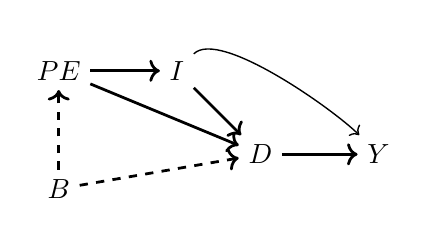
\begin{tikzpicture}[node distance=1.5cm]
% nodes %
\node[text centered] (d) {$D$};
\node[right of = d, text centered] (y) {$Y$};
\node[above left of = d, text centered] (i) {$I$};
\node[left of = i, text centered] (pe) {$PE$};
\node[below of = pe, text centered] (b) {$B$};
% edges %
\draw[->, line width= 1] (d) -- (y);
\draw[->, line width= 1,] (i) -- (d);
\draw[->, line width= 1,] (pe) -- (i);
\draw[->, line width= 1,] (pe) -- (d);
\draw[->, line width= 1, dashed] (b) -- (pe);
\draw[->, line width= 1, dashed] (b) -- (d);
\draw[->, line width= .5] (i) to [out=45,in=135, looseness=0.5] (y);
\end{tikzpicture}
	\end{center}$PE$ is parental education, $B$ is ``unobserved background factors (i.e., ``ability'')'', $I$ is family income, $D$ is college education and $Y$ is log wages.  The DAG is an approximation of Becker's underlying (causal) human capital model. 


\end{frame}


\begin{frame}[plain]
\begin{center}
\textbf{Arrows, but also \emph{missing arrows}}
\end{center}

Before we dive into all this notation, couple of things
\begin{center}
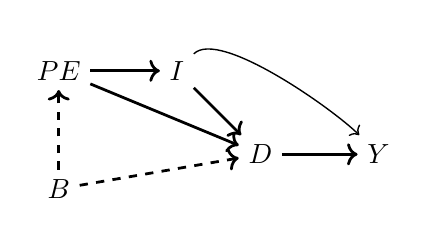
\begin{tikzpicture}[node distance=1.5cm]
% nodes %
\node[text centered] (d) {$D$};
\node[right of = d, text centered] (y) {$Y$};
\node[above left of = d, text centered] (i) {$I$};
\node[left of = i, text centered] (pe) {$PE$};
\node[below of = pe, text centered] (b) {$B$};
% edges %
\draw[->, line width= 1] (d) -- (y);
\draw[->, line width= 1,] (i) -- (d);
\draw[->, line width= 1,] (pe) -- (i);
\draw[->, line width= 1,] (pe) -- (d);
\draw[->, line width= 1, dashed] (b) -- (pe);
\draw[->, line width= 1, dashed] (b) -- (d);
\draw[->, line width= .5] (i) to [out=45,in=135, looseness=0.5] (y);
\end{tikzpicture}
	\end{center}$PE$ and $D$ are caused by $B$. But why doesn't $B$ cause $Y$?? Do you believe this?  Why/why not?  We can dispute this, but notice -- we can see the assumption, which is transparent and communicates the author's beliefs, as well as the needed assumptions in their forthcoming \emph{empirical} model. Every empirical strategy makes assumptions, but oftentimes they are not as transparent to us as this is.


\end{frame}


\begin{frame}[plain]

\begin{center}
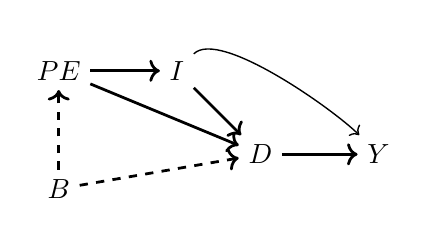
\begin{tikzpicture}[node distance=1.5cm]
% nodes %
\node[text centered] (d) {$D$};
\node[right of = d, text centered] (y) {$Y$};
\node[above left of = d, text centered] (i) {$I$};
\node[left of = i, text centered] (pe) {$PE$};
\node[below of = pe, text centered] (b) {$B$};
% edges %
\draw[->, line width= 1] (d) -- (y);
\draw[->, line width= 1,] (i) -- (d);
\draw[->, line width= 1,] (pe) -- (i);
\draw[->, line width= 1,] (pe) -- (d);
\draw[->, line width= 1, dashed] (b) -- (pe);
\draw[->, line width= 1, dashed] (b) -- (d);
\draw[->, line width= .5] (i) to [out=45,in=135, looseness=0.5] (y);
\end{tikzpicture}
\end{center}	
	
	\begin{itemize}
		\item $B$ is a \textbf{parent} of $PE$ and $D$
		\item $PE$ and $D$ are \textbf{descendants} of $B$
		\item There is a \textbf{direct (causal) path} from $D$ to $Y$
		\item There is a \textbf{mediated (causal) path} from $B$ to $Y$ through $D$
		\item There are four \textbf{paths} from $PE$ to $Y$ but none are direct, and one is unlike the others
	\end{itemize}
\end{frame}


\begin{frame}[plain]
\begin{center}
\textbf{Colliders}
\end{center}

\begin{center}
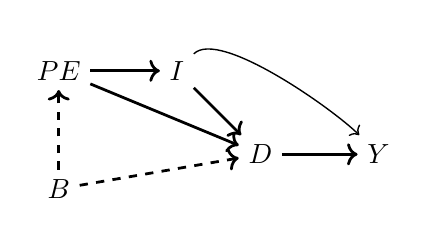
\begin{tikzpicture}[node distance=1.5cm]
% nodes %
\node[text centered] (d) {$D$};
\node[right of = d, text centered] (y) {$Y$};
\node[above left of = d, text centered] (i) {$I$};
\node[left of = i, text centered] (pe) {$PE$};
\node[below of = pe, text centered] (b) {$B$};
% edges %
\draw[->, line width= 1] (d) -- (y);
\draw[->, line width= 1,] (i) -- (d);
\draw[->, line width= 1,] (pe) -- (i);
\draw[->, line width= 1,] (pe) -- (d);
\draw[->, line width= 1, dashed] (b) -- (pe);
\draw[->, line width= 1, dashed] (b) -- (d);
\draw[->, line width= .5] (i) to [out=45,in=135, looseness=0.5] (y);
\end{tikzpicture}
\end{center}	

Notice anything different with this DAG?  Look closely.
\begin{itemize}

		\item $D$ is a \textbf{collider} along the path $B\rightarrow D\leftarrow I$ (i.e., ``colliding'' at $D$)
		\item $D$ is a \textbf{noncollider} along the path $B\rightarrow D\rightarrow Y$

\end{itemize}

\end{frame}


\begin{frame}[plain]
\begin{center}
\textbf{Summarizing Value of DAGs imo}
\end{center}

\begin{enumerate}
\item Facilitates the task of designing identification strategy for estimating average causal effects
\item Facilitates the task of testing compatibility of the model with your data
\item Visualizes the identifying assumptions which opens up the model to critical scrutiny
\end{enumerate}

\end{frame}

\begin{frame}[plain]
\begin{center}
\textbf{Creating DAGs}
\end{center}

\begin{itemize}
		\item The DAG is a \emph{relevant} causal relationships describing the relationship between $D$ and $Y$
		\item It will include:
		\begin{itemize}
			\item All direct causal effects among the \emph{relevant} variables in the graph
			\item All common causes of any pair of \emph{relevant} variables in the graph
		\end{itemize}
		\item No need to model a dinosaur stepping on a bug causing in a million years some evolved created that impacted your decision to go to college
		\item We get ideas for DAGs from theory, models, observation, experience, prior studies, intuition
		\item Sometimes called the data generating process.
\end{itemize}

\end{frame}



\subsubsection{Designing identification strategies}

\begin{frame}[plain]
	\begin{center}
	\textbf{Confounding}
	\end{center}

	\begin{itemize}
		\item Omitted variable bias has a name in DAGs: ``confounding''
		\item Confounding occurs when when the treatment and the outcomes have a common cause or parent which creates spurious correlation between $D$ and $Y$
		
		\begin{center}
		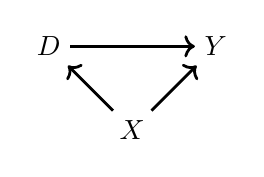
\begin{tikzpicture}
			[node distance=1.5cm]
		% nodes %
		\node[text centered] (d) {$D$};
		\node[below right of = d, text centered] (x) {$X$};
		\node[above right of = x, text centered] (y) {$Y$};
 
		% edges %
		\draw[->, line width= 1] (d) -- (y);
		\draw[->, line width= 1] (x) -- (d);
		\draw[->, line width= 1] (x) -- (y);
		\end{tikzpicture}
		\end{center}
		
		The \emph{correlation} between $D$ and $Y$ no longer reflects the causal effect of $D$ on $Y$
	\end{itemize}
\end{frame}

\begin{frame}[plain]
\begin{center}
\textbf{Backdoor Paths}
\end{center}

\begin{itemize}
		\item Confounding creates \textbf{backdoor paths} between treatment and outcome ($D\leftarrow X\rightarrow Y$) -- i.e., spurious correlations
		\item Not the same as mediation ($D \rightarrow X \rightarrow Y$)
		\item We can ``block'' backdoor paths by conditioning on the common cause $X$
		\item Once we condition on $X$, the correlation between $D$ and $Y$ estimates the causal effect of $D$ on $Y$
		\item Conditioning means calculating $E[Y|D=1,X]-E[Y|D=0,X]$ for each value of $X$ then combining (e.g., integrating)

\end{itemize}	
	
		\begin{center}
		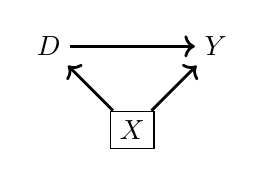
\begin{tikzpicture}
			[node distance=1.5cm]
		% nodes %
		\node[text centered] (d) {$D$};
		\node[below right of = d, text centered, rectangle, draw, thin] (x) {$X$};
		\node[above right of = x, text centered] (y) {$Y$};
 
		% edges %
		\draw[->, line width= 1] (d) -- (y);
		\draw[->, line width= 1] (x) -- (d);
		\draw[->, line width= 1] (x) -- (y);
		\end{tikzpicture}
		\end{center}
	
\end{frame}


\begin{frame}[plain]
\begin{center}
\textbf{Blocked backdoor paths}
\end{center}

	A backdoor path is blocked if and only if:
	\begin{itemize}
		\item It contains a noncollider that has been conditioned on
		\item Or it contains a collider that has not been conditioned on 
	\end{itemize}

\end{frame}


\begin{frame}[plain]
	\begin{center}
	\textbf{Examples of blocked paths}
	\end{center}
	
	Examples:
	\begin{enumerate}
		\item Conditioning on a noncollider blocks a path:

		\begin{center}
		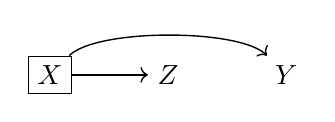
\begin{tikzpicture}
		[node distance=1.5cm]
		% nodes %
		\node[text centered, rectangle, draw, thin] (x) {$X$};
		\node[right of = x, text centered] (z) {$Z$};
		\node[right of = z, text centered] (y) {$Y$};
 
		% edges %
		\draw[->, line width= .5] (x) -- (z);
		\draw[->, line width= .5] (x) to [out=45,in=135, looseness=0.5] (y);
		\end{tikzpicture}
		\end{center}

		\item Conditioning on a collider opens a path (i.e., creates spurious correlations):

		\begin{center}
		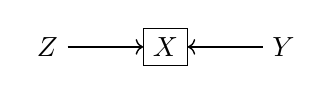
\begin{tikzpicture}
		[node distance=1.5cm]
		% nodes %
		\node[text centered] (z) {$Z$};
		\node[right of = z, text centered, rectangle, draw, thin] (x) {$X$};
		\node[right of = x, text centered] (y) {$Y$};
 
		% edges %
		\draw[->, line width= .5] (z) -- (x);
		\draw[->, line width= .5] (y) -- (x);
		\end{tikzpicture}
		\end{center}

		\item \emph{Not} conditioning on a collider blocks a path:

		\begin{center}
		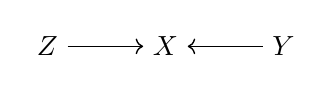
\begin{tikzpicture}
		[node distance=1.5cm]
		% nodes %
		\node[text centered] (z) {$Z$};
		\node[right of = z, text centered] (x) {$X$};
		\node[right of = x, text centered] (y) {$Y$};
 
		% edges %
		\draw[->, line width= .5] (z) -- (x);
		\draw[->, line width= .5] (y) -- (x);
		\end{tikzpicture}
		\end{center}

	\end{enumerate}
\end{frame}


\begin{frame}[plain]

	\begin{center}
	\textbf{Backdoor criterion}
	\end{center}
	

		\begin{block}{Backdoor criterion}
		Conditioning on $X$ satisfies the backdoor criterion with respect to $(D,Y)$ directed path if:
		\begin{enumerate}
			\item All backdoor paths are blocked by $X$
			\item No element of $X$ is a collider 
		\end{enumerate}

		In words: If $X$ satisfies the backdoor criterion with respect to $(D,Y)$, then controlling for or matching on $X$ identifies the causal effect of $D$ on $Y$
		\end{block}
\end{frame}

\begin{frame}[plain]
\begin{center}
\textbf{What control strategy meets the backdoor criterion?}
\end{center}
		\begin{itemize}
			\item List all backdoor paths from $D$ to $Y$. I'll wait.

			\begin{center}
			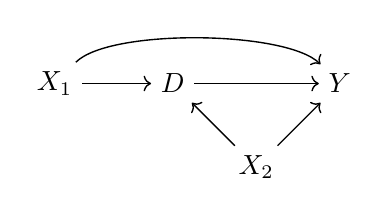
\begin{tikzpicture}
			[node distance=1.5cm]
			% nodes %
			\node[text centered,rectangle,thin] (x1) {$X_1$};
			\node[right of = x1, text centered] (d) {$D$};
			\node[below right of = d, text centered] (x2) {$X_2$};
			\node[above right of = x2, text centered] (y) {$Y$};
 
			% edges %
			\draw[->, line width= .5] (x1) -- (d);
			\draw[->, line width= .5] (d) -- (y);
			\draw[->, line width= .5] (x2) -- (d);
			\draw[->, line width= .5] (x2) -- (y);
			\draw[->, line width= .5] (x1) to [out=45,in=135, looseness=0.5] (y);
			\end{tikzpicture}
			\end{center}

			\item What are the necessary and sufficient set of controls which will satisfy the backdoor criterion?
		\end{itemize}
		
		\framebreak
		



\end{frame}


\begin{frame}[plain]
\begin{center}
\textbf{What if you have an unobservable?}
\end{center}


		\begin{itemize}
			\item List all the backdoor paths from $D$ to $Y$.
			
			\begin{center}
			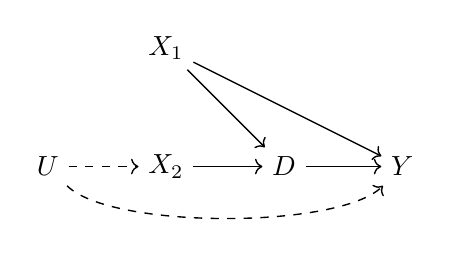
\begin{tikzpicture}
			[node distance=1.5cm]
			% nodes %
			\node[text centered] (u) {$U$};
			\node[right of = u, text centered] (x2) {$X_2$};
			\node[above of = x2, text centered] (x1) {$X_1$};
			\node[right of = x2, text centered] (d) {$D$};
			\node[right of = d, text centered] (y) {$Y$};
 
			% edges %
			\draw[->, line width= .5, dashed] (u) -- (x2);
			\draw[->, line width= .5] (x2) -- (d);
			\draw[->, line width= .5] (x1) -- (d);
			\draw[->, line width= .5] (x1) -- (y);
			\draw[->, line width= .5] (d) -- (y);
			\draw[->, line width= .5, dashed] (u) to [out=-45,in=-135, looseness=0.5] (y);
			\end{tikzpicture}
			\end{center}

			\item What are the necessary and sufficient set of controls which will satisfy the backdoor criterion?
			\item What about the unobserved variable, $U$?
		\end{itemize}
		
		\framebreak
		
	
\end{frame}

\begin{frame}[plain]
\begin{center}
\textbf{Multiple strategies}
\end{center}

			
			\begin{center}
			\begin{tikzpicture}
			[node distance=1.5cm, text centered]
			% nodes %
			\node[] (x3) {$X_3$};
			\node[above left of = x3,rectangle,draw,thin] (x1) {$X_1$};
			\node[below left of = x3,rectangle,draw,thin] (x2) {$X_2$};
			\node[right of = x] (d) {$D$};
			\node[right of = d] (y) {$Y$};
 
			% edges %
			\draw[->, line width= .5] (x1) -- (x3);
			\draw[->, line width= .5] (x2) -- (x3);
			\draw[->, line width= .5] (x1) to [out=0,in=135, looseness=0.5] (y);
			\draw[->, line width= .5] (x2) to [out=0,in=-135, looseness=0.5] (y);
			\draw[->, line width= .5] (x3) -- (d);
			\draw[->, line width= .5] (d) -- (y);
			\end{tikzpicture}

			\begin{tikzpicture}
			[node distance=1.5cm, text centered]
			% nodes %
			\node[rectangle,draw,thin] (x3) {$X_3$};
			\node[above left of = x3] (x1) {$X_1$};
			\node[below left of = x3] (x2) {$X_2$};
			\node[right of = x] (d) {$D$};
			\node[right of = d] (y) {$Y$};
 
			% edges %
			\draw[->, line width= .5] (x1) -- (x3);
			\draw[->, line width= .5] (x2) -- (x3);
			\draw[->, line width= .5] (x1) to [out=0,in=135, looseness=0.5] (y);
			\draw[->, line width= .5] (x2) to [out=0,in=-135, looseness=0.5] (y);
			\draw[->, line width= .5] (x3) -- (d);
			\draw[->, line width= .5] (d) -- (y);
			\end{tikzpicture}
			\end{center}
			
		\begin{itemize}
			\item Conditioning on the common causes, $X_1$ and $X_2$, is sufficient
			\item \dots but so is conditioning on $X_3$ 
		\end{itemize}
\end{frame}

\begin{frame}[plain]

\begin{center}
\textbf{Testing the Validity of the DAG}
\end{center}

\begin{itemize}
\item The DAG makes testable predictions
\item Conditional on $D$ and $I$, parental education ($PE$) should no longer be correlated with $Y$
\item Can be hard to figure this out by hand, but software can help (e.g., Daggity.net is browser based)
\end{itemize}

\begin{center}
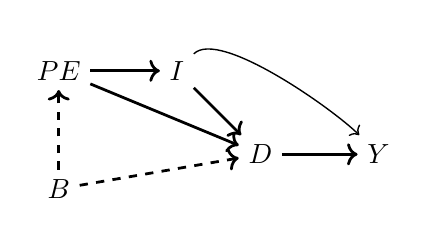
\begin{tikzpicture}[node distance=1.5cm]
% nodes %
\node[text centered] (d) {$D$};
\node[right of = d, text centered] (y) {$Y$};
\node[above left of = d, text centered] (i) {$I$};
\node[left of = i, text centered] (pe) {$PE$};
\node[below of = pe, text centered] (b) {$B$};
% edges %
\draw[->, line width= 1] (d) -- (y);
\draw[->, line width= 1,] (i) -- (d);
\draw[->, line width= 1,] (pe) -- (i);
\draw[->, line width= 1,] (pe) -- (d);
\draw[->, line width= 1, dashed] (b) -- (pe);
\draw[->, line width= 1, dashed] (b) -- (d);
\draw[->, line width= .5] (i) to [out=45,in=135, looseness=0.5] (y);
\end{tikzpicture}
\end{center}	

\end{frame}


\begin{frame}[plain]

\begin{figure}
\centering
\includegraphics[scale=0.05]{./lecture_includes/daggity.jpg}
\end{figure}

\end{frame}





\subsubsection{Conditioning on a collider}

\begin{frame}[allowframebreaks,plain]
	\begin{center}
	\textbf{Collider bias}
	\end{center}

		\begin{itemize}
		\item \textbf{Conditioning on a collider introduces spurious correlations; can even mask causal directions}
			\begin{itemize}
			\item There is only one backdoor path from $D$ to $Y$

			\begin{center}
			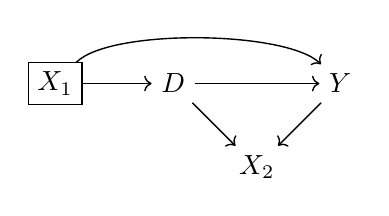
\begin{tikzpicture}
			[node distance=1.5cm]
			% nodes %
			\node[text centered,draw,rectangle,thin] (x1) {$X_1$};
			\node[right of = x1, text centered] (d) {$D$};
			\node[below right of = d, text centered] (x2) {$X_2$};
			\node[above right of = x2, text centered] (y) {$Y$};
 
			% edges %
			\draw[->, line width= .5] (x1) -- (d);
			\draw[->, line width= .5] (d) -- (y);
			\draw[->, line width= .5] (d) -- (x2);
			\draw[->, line width= .5] (y) -- (x2);
			\draw[->, line width= .5] (x1) to [out=45,in=135, looseness=0.5] (y);
			\end{tikzpicture}
			\end{center}
			
			\item Conditioning on $X_1$ blocks the backdoor path

			\item But what if we also condition on $X_2$?

			\begin{center}
			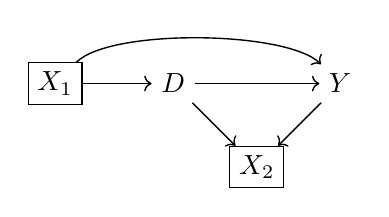
\begin{tikzpicture}
			[node distance=1.5cm]
			% nodes %
			\node[text centered,draw,rectangle,thin] (x1) {$X_1$};
			\node[right of = x1, text centered] (d) {$D$};
			\node[below right of = d, draw, rectangle, text centered] (x2) {$X_2$};
			\node[above right of = x2, text centered] (y) {$Y$};

			% edges %
			\draw[->, line width= .5] (x1) -- (d);
			\draw[->, line width= .5] (d) -- (y);
			\draw[->, line width= .5] (d) -- (x2);
			\draw[->, line width= .5] (y) -- (x2);
			\draw[->, line width= .5] (x1) to [out=45,in=135, looseness=0.5] (y);
			\end{tikzpicture}
			\end{center}
			
			\item Conditioning on $X_2$ opens up a new path, creating new spurious correlations between $D$ and $Y$
			\end{itemize}

		\framebreak

		
		\item \textbf{Even controlling for pretreatment covariates can create bias}
			\begin{itemize}
			\item Name the backdoor paths.  Is it open or closed?
			
			\begin{center}
			\begin{tikzpicture}
			[node distance=1.5cm, text centered]
			% nodes %
			\node[] (x) {$X$};
			\node[above left of = x] (u1) {$U_1$};
			\node[below left of = x] (u2) {$U_2$};
			\node[right of = x] (d) {$D$};
			\node[right of = d] (y) {$Y$};
 
			% edges %
			\draw[->, line width= .5, dashed] (u1) -- (x);
			\draw[->, line width= .5, dashed] (u2) -- (x);
			\draw[->, line width= .5, dashed] (u1) to [out=0,in=135, looseness=0.5] (y);
			\draw[->, line width= .5, dashed] (u2) to [out=0,in=-135, looseness=0.5] (d);
			\draw[->, line width= .5] (d) -- (y);
			\end{tikzpicture}
			\end{center}
			
			\item But what if we condition on $X$? 

			\begin{center}
			\begin{tikzpicture}
			[node distance=1.5cm, text centered]
			% nodes %
			\node[text centered,draw,rectangle,thin] (x) {$X$};
			\node[above left of = x] (u1) {$U_1$};
			\node[below left of = x] (u2) {$U_2$};
			\node[right of = x] (d) {$D$};
			\node[right of = d] (y) {$Y$};
 
			% edges %
			\draw[->, line width= .5, dashed] (u1) -- (x);
			\draw[->, line width= .5, dashed] (u2) -- (x);
			\draw[->, line width= .5, dashed] (u1) to [out=0,in=135, looseness=0.5] (y);
			\draw[->, line width= .5, dashed] (u2) to [out=0,in=-135, looseness=0.5] (d);
			\draw[->, line width= .5] (d) -- (y);
			\end{tikzpicture}
			\end{center}


			\end{itemize}
		\end{itemize}		
		\framebreak


\end{frame}

\begin{frame}[plain]
\begin{center}
\textbf{Living in reality - he doesn't love you}
\end{center}

\begin{itemize}

\item \textbf{Fact \#1}: We can't know if we have a collider bias (confounder) problem without making assumptions about the causal model (i.e. not in the codebook)
\item \textbf{Fact \# 2}: You can't just haphazardly throw in a bunch of controls on the RHS (i.e., ``the kitchen sink'') bc you may inadvertently be conditioning on a collider which can lead to massive biases
\item \textbf{Fact \# 3}: You have no choice but to leverage economic theory, intuition, intimate familiarity with institutional details and background knowledge for research designs.  
\item \textbf{Fact \#4}: You can only estimate causal effects with \textbf{data} and \textbf{assumptions}.
\end{itemize}

\end{frame}


%\begin{frame}[plain]
%\begin{center}
%\textbf{Fryer forthcoming JPE}
%\end{center}

%\begin{itemize}
%\item Consider Fryer \emph{forthcoming JPE} which finds no evidence for racial bias in police shooting using police arrest administrative data.  
%\item But what gets you stopped in the first place?  What gets you in the sample?  Race.
%\item If officers have a higher threshold for stopping whites as a result of racial bias during an unseen first stage of police-citizen contact, the white civilians in the data will not be comparable to the black civilians and may lead to a faulty conclusion of no racial bias in police behavior (see Knox, Lowe and Mummolo 2019)
%\item Let's look at some examples and simulations to illustrate this.
%\end{itemize}

%\end{frame}


\begin{frame}[plain]
\begin{center}
\textbf{Examples of collider bias}
\end{center}

\end{frame}


\begin{frame}[plain]
\begin{center}
\textbf{Bad controls}
\end{center}

\begin{itemize}
\item Angrist and Pischke in MHE talk about a specific type of danger associated with controlling for an outcome -- ``bad controls''
\item The problem is not controlling for an outcome;
\item The problem is controlling for a collider and don't correct for \emph{that}
\item This has implications for when you work with non-random administrative data, too
\end{itemize}

\end{frame}

\begin{frame}[plain]
	\begin{center}
	\textbf{Sample selection example of collider bias}
	\end{center}

	\alert{Important}: Since unconditioned colliders block back-door paths, what exactly does conditioning on a collider do? Let's illustrate with a fun example and some made-up data\\
	\begin{itemize}
	\item \underline{CNN.com} headline: Megan Fox voted worst -- but sexiest -- actress of 2009 \myurlshort{http://marquee.blogs.cnn.com/2009/12/30/megan-fox-voted-worst-but-sexiest-actress-of-2009/}{(link)}
	\item Are these two things actually negatively correlated in the world?
	\item Assume talent and beauty are independent, but each causes someone to become a movie star.  What's the correlation between talent and beauty for a sample of movie stars compared to the population as a whole (stars and non-stars)?
	\end{itemize}

\end{frame}


\begin{frame}[plain]

\begin{itemize}
	\item What if the sample consists \emph{only} of movie stars?
\end{itemize}	

	\begin{center}
	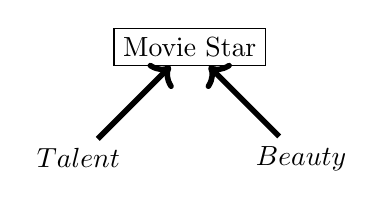
\begin{tikzpicture}
	[node distance=2cm, text centered]
	
	%nodes
	\node[text centered,draw,rectangle,thin] (x) {Movie Star};
	\node[below left of = x] (u1) {$Talent$};
	\node[below right of = x] (u2) {$Beauty$};

			% edges %
			\draw[->, line width= 2] (u1) -- (x);
			\draw[->, line width= 2] (u2) -- (x);
			\end{tikzpicture}
			\end{center}




\end{frame}

\begin{frame}[plain]
	\begin{center}
	\textbf{Stata code}
	\end{center}

\scriptsize{
\texttt{clear all \\
set seed 3444 \\
\bigskip
* 2500 independent draws from standard normal distribution \\
set obs 2500 \\
generate beauty=rnormal() \\
generate talent=rnormal() \\
\bigskip
* Creating the collider variable (star) \\
gen score=(beauty+talent) \\
egen c85=pctile(score), p(85)   \\
gen star=(score$>=$c85) \\
label variable star "Movie star" \\
\bigskip
* Conditioning on the top 15\% \\
twoway (scatter beauty talent, mcolor(black) msize(small) msymbol(smx)), ytitle(Beauty) xtitle(Talent) subtitle(Aspiring actors and actresses) by(star, total)}}

		\framebreak


\end{frame}

\begin{frame}[shrink=20,plain]

	\begin{figure}
	\includegraphics[height=9cm]{./lecture_includes/beauty_collider.pdf}     
	\caption{Top left figure: Non-star sample scatter plot of beauty (vertical axis) and talent (horizontal axis). Top right right figure: Star sample scatter plot of beauty and talent.  Bottom left figure: Entire (stars and non-stars combined) sample scatter plot of beauty and talent.}
	\end{figure}
\end{frame}


\begin{frame}[plain]
\begin{center}
\textbf{Stata}
\end{center}

\begin{itemize}
\item Run Stata file star.do
\end{itemize}

\end{frame}


\begin{frame}[plain]
\begin{center}
\textbf{Occupational sorting and discrimination example of collider bias}
\end{center}

\begin{itemize}
\item Let's look at another example: very common for think tanks and journalists to say that the gender gap in earnings disappears once you control for occupation.
\item But what if occupation is a collider, which it could be in a model with occupational sorting
\item Then controlling for occupation in a wage regression searching for discrimination can lead to all kinds of crazy results \emph{even in a simulation where we explicitly design there to be discrimination}
\end{itemize}

\end{frame}

\begin{frame}[plain]
\begin{center}
\textbf{DAG}
\end{center}

\begin{center}
	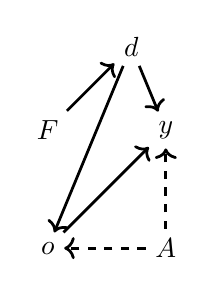
\begin{tikzpicture}
	[node distance=1.5cm]
	% nodes %
	\node[text centered] (f) {$F$};
	\node[above right of = f, text centered] (d) {$d$};
	\node[right of = f] (y) {$y$};
	\node[below  of = f, text centered] (o) {$o$};
	\node[right of = o, text centered] (a) {$A$};
 
	% edges %
	\draw[->, line width= 1] (f) -- (d);
	\draw[->, line width= 1] (d) -- (o);
	\draw[->, line width= 1, dashed] (a) -- (o);

	\draw[->, line width= 1] (d) -- (y);
	\draw[->, line width= 1] (o) -- (y);
	\draw[->, line width= 1, dashed] (a) -- (y);

	\end{tikzpicture}
	\end{center}
	
$F$ is female, $d$ is discrimination, $o$ is occupation, $y$ is earnings and $A$ is ability. Dashed lines mean the variable cannot be observed. Note, by design, being a female has no effect on earnings or occupation, and has no relationship with ability. So earnings is coming through discrimination, occupation, and ability. 

\end{frame}


\begin{frame}[plain]

\begin{center}
	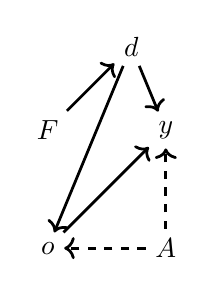
\begin{tikzpicture}
	[node distance=1.5cm]
	% nodes %
	\node[text centered] (f) {$F$};
	\node[above right of = f, text centered] (d) {$d$};
	\node[right of = f] (y) {$y$};
	\node[below  of = f, text centered] (o) {$o$};
	\node[right of = o, text centered] (a) {$A$};
 
	% edges %
	\draw[->, line width= 1] (f) -- (d);
	\draw[->, line width= 1] (d) -- (o);
	\draw[->, line width= 1, dashed] (a) -- (o);

	\draw[->, line width= 1] (d) -- (y);
	\draw[->, line width= 1] (o) -- (y);
	\draw[->, line width= 1, dashed] (a) -- (y);

	\end{tikzpicture}
	\end{center}


Mediation and Backdoor paths

\begin{enumerate}

\item $d$ $\rightarrow o \rightarrow y$
\item $d$ $\rightarrow o \leftarrow A \rightarrow y$
\end{enumerate}

\end{frame}

\begin{frame}[plain]
\begin{center}
\textbf{Stata model (Erin Hengel)}
\end{center}

\begin{itemize}

\item Erin Hengel (\url{www.erinhengel.com}) and I worked out this code and she gave me permission to put in my Mixtape
\item Let's look at collider\_discrimination.do or collider\_discrimination.R together
\end{itemize}

\end{frame}

\begin{frame}[plain, shrink=20]

\begin{table}[htbp]\centering
\scriptsize
\caption{Regressions illustrating collider bias with simulated gender disparity}
\begin{center}
\begin{tabular}{l*{3}{c}}
\toprule
\multicolumn{1}{l}{Covariates: }&
\multicolumn{1}{c}{\textbf{Unbiased combined effect}}&
\multicolumn{1}{c}{\textbf{Biased }}&
\multicolumn{1}{c}{\textbf{Unbiased wage effect only}}\\
\midrule
Female                 	&	-3.074***	&	0.601*** 	& -0.994*** \\
                    		&	(0.000)	&	(0.000)	& (0.000) \\
Occupation		&			&	1.793*** 	& 0.991*** \\
                 	   	&			&	(0.000)	& (0.000) \\
Ability			&			&			& 2.017*** \\
				&			&			& (0.000) \\
\\
\midrule
N                   &       10,000   &       10,000   &       10,000   \\
Mean of dependent variable&      0.45   &      0.45  & 0.45  \\
\bottomrule
\end{tabular}
\end{center}
\end{table}

\begin{itemize}
\item Recall we designed there to be a discrimination coefficient of -1
\item If we do not control for occupation, then we get the combined effect of $d \rightarrow o \rightarrow y$ and $d  \rightarrow y$
\item Because it seems intuitive to control for occupation, notice column 2 - the sign flips!
\item We are only able to isolate the direct causal effect by conditioning on ability and occupation, but ability is unobserved
\end{itemize}

\end{frame}

\begin{frame}[plain]
\begin{center}
\textbf{Administrative data}
\end{center}

\begin{itemize}
\item Admin data has become extremely common, if not absolutely necessary 
\item But naive use of admin data can be dangerous if the drawing of the sample is itself a collider problem (Heckman 1979; Elwert and Winship 2014)
\item Let's look at a new paper by Fryer (2019) and a critique by Knox, et al. (2019)
\end{itemize}

\end{frame}

\begin{frame}[plain]
\begin{center}
\textbf{Collider bias and police use of force}
\end{center}

\begin{itemize}
\item Claims of excessive and discriminator use of police force against minorities (e.g., Black Lives Matter, Trayvon Martin, Michael Brown, Eric Garner)
\item Challenging to identify
	\begin{itemize}
	\item Police-citizen interactions are conditional on interactions having already been triggered
	\item That initial interaction is unobserved
	\end{itemize}
\item Fryer (2019) is a monumental study for its data collection and analysis: Stop and Frisk, Police-Public Contact Survey, and admin data from two jurisdictions
\item Codes up almost 300 variables from arrest narratives which range from 2-100 pages in length -- shoeleather!
\end{itemize}

\end{frame}


\begin{frame}[plain]
\begin{center}
\textbf{Initial interaction}
\end{center}

\begin{itemize}
\item Fryer finds that blacks and Hispanics were more than 50\% more likely to have an interaction with the policy in NYC Stop and Frisk as well as Police-Public Contact survey \item It survives extensive controls -- magnitudes fall, but still very large (21\%)
\item Moves to admin data 
\item Conditional on police interaction, \emph{no} racial differences in officer-related shootings
\item Fryer calls it one of the most surprising findings in his career
\item Lots of eyes on this study as a result of the counter intuitive results; published in JPE
\item Knox, et al (202) claim his data is itself a collider.  What?
\end{itemize}

\end{frame}

\begin{frame}[plain]

\begin{center}
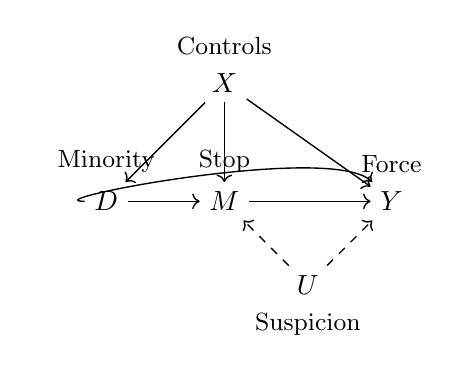
\begin{tikzpicture}[node distance=1.5cm]
% nodes %
\node[label={\small Minority},text centered] (d) {$D$};
\node[right of = d, label={\small Stop}, text centered] (m) {$M$};
\node[below right of = m, label=below:{\small Suspicion}, text centered] (u) {$U$};
\node[above right of = u, label={\small Force}, text centered] (y) {$Y$};
\node[above of = m, label={\small Controls}, text centered] (x) {$X$};
% edges %
\draw[->, line width= .5] (x) -- (d);
\draw[->, line width= .5] (x) -- (y);
\draw[->, line width= .5] (d) -- (m);
\draw[->, line width= .5] (x) -- (m);
\draw[->, line width= .5] (m) -- (y);
\draw[->, line width= .5, dashed] (u) -- (m);
\draw[->, line width= .5, dashed] (u) -- (y);
\draw[->, line width= .5] (d) to [out=180,in=135, looseness=0.5] (y);
\end{tikzpicture}
\end{center}Fryer told us $D \rightarrow M$ exists from both Stop and Frisk and Police-Public.  But note: admin data is instances of $M$ stops, which is itself a collider. If this DAG is true, then spurious correlations enter between $M$ and $Y$ which may dilute our ability to estimate causal effects.

\end{frame}


\begin{frame}[plain]
\begin{center}
\textbf{Knox, et al (2020)}
\end{center}

\begin{itemize}
\item Move from DAG to more contemporary potential outcomes notation to design relevant parameters
\item Use potential outcomes and bounds
\item Even with lower bound estimates of the incidence of police violence against civilians is more than 5x higher than what Fryer (2019) finds
\item Heckman (1979) -- we \emph{cannot} afford to ignore sample selection
\end{itemize}

\end{frame}





\begin{frame}[plain]
\begin{center}
\textbf{Summarizing all of this}
\end{center}

\begin{itemize}
\item Your dataset will not come with a codebook flagging some variables as ``confounders'' and other variables as ``colliders'' because those terms are always context specific
\item Except for some unique situations that aren't generally applicable, you also don't always know statistically you have an omitted variable bias problem; but both of these are fatal for any application
\item You only know to do what you're doing based on \emph{knowledge about data generating process}. 
\item All identification must be guided by theory, experience, observation, common sense and knowledge of institutions 
\item DAGs absorb that information and can be then used to write out the explicit identifying model
\end{itemize}

\end{frame}

\begin{frame}[plain]
\begin{center}
\textbf{DAGs are not panacea}
\end{center}

\begin{itemize}
\item DAGs cannot handle, though, reverse causality or simultaneity
\item So there are limitations.  ``All models are wrong but some are useful''
\item They are also not popular (see Twitter ongoing debates which have descended into light hearted jokes as well as aggressive debates)
\item But I think they are helpful and while not \emph{necessary}, showcase what is necessary -- assumptions
\item Heckman (1979) can maybe provide some justification at times
\end{itemize}

\end{frame}


\section{Regression discontinuity designs}

\subsection{Introduction}



\begin{frame}

	\begin{center}
	\textbf{What is regression discontinuity design?}
	\end{center}
	
Very popular particular type of research design known as \emph{regression discontinuity design} (RDD).  Cook (2008) has a fascinating history of thought on how and why. 
		\begin{itemize}
		\item  Donald Campbell, educational psychologist, invented regression discontinuity design (Thistlethwaite and Campbell, 1960), but then it went dormant for decades (Cook 2008).  
		\item Angrist and Lavy (1999) and Black (1999) independently rediscover it. It's become incredibly popular in economics
		\end{itemize}
\end{frame}

\begin{frame}[plain]

	\begin{figure}
	\makebox[\textwidth][c]{\includegraphics[width=0.8\textwidth]{./lecture_includes/RDD_overtime.jpg}}%
	\end{figure}

\end{frame}

%\begin{frame}[plain]
%	\begin{center}
%	\textbf{Tell me what you think is happening}
%	\end{center}
	
%	\begin{figure}
%  \makebox[\textwidth][c]{\includegraphics[width=1.2\textwidth]{./lecture_includes/carpenter_aej.pdf}}%
%	\end{figure}
%\end{frame}


\begin{frame}[plain]
	\begin{center}
	\textbf{Tell me what you think is happening}
	\end{center}
	
	\begin{figure}
  \makebox[\textwidth][c]{\includegraphics[width=1\textwidth]{./lecture_includes/rdd_hoekstra1}}%
	\end{figure}
\end{frame}
	
	
\begin{frame}[plain]
	\begin{center}
	\textbf{Tell me what you think is happening}
	\end{center}
	
	\begin{figure}
  \makebox[\textwidth][c]{\includegraphics[width=1.2\textwidth]{./lecture_includes/rdd_hoekstra2}}%
	\end{figure}
\end{frame}




\begin{frame}[plain]
	\begin{center}
	\textbf{What is a regression discontinuity design?}
	\end{center}

	\begin{itemize}	
	\item We want to estimate some causal effect of a treatment on some outcome, but we're worried about selection bias $$E[Y^0|D=1] \neq E[Y^0 | D=0]]$$due to self-selection into treatment
	\item RDD is based on a idea:  if treatment assignment occurs abruptly when some underlying variable $X$ called the ``running variable'' passes a cutoff $c_0$, then we can use that to estimate the causal effect \emph{even of a self-selected treatment}
	\end{itemize}
\end{frame}

\begin{frame}[plain]
	\begin{center}
	\textbf{Running and jumping}
	\end{center}
	
	\begin{itemize}
	\item Firms, schools and govt agencies have running variables that are used to assign treatments in their rules
	\item And consequently, probabilities of treatment will ``jump'' when that running variable exceeds a known threshold
	\item  Most effective RDD studies involve programs where running variables assign treatments based on a ``hair trigger''  
	\item Good reasons; inexplicable reasons; arbitrary rules; a choice made by necessity and resource constraints; natural experiments
	\end{itemize}
\end{frame}

	



\begin{frame}[plain]
\begin{center}
\textbf{Selection examples and solutions from the literature}
\end{center}

Think of these in light of a treatment where $E[Y^0 | D=1] \neq E[Y^0 | D=0]$
		\begin{itemize}
		\item Yelp rounded a continuous score of ratings to generate stars which Anderson and Magruder 2011 used to study firm revenue
		\item US targeted air strikes in Vietnam using rounded risk scores which Dell and Querubin 2018 used to study the military and political activities of the communist state
		\item Card, Dobkin, and Maeskas 2008 studied the effect of universal healthcare on mortality and healthcare usage exploiting jumps at age 65
		\item Almond, et al. 2010 studied the effect of intensive medical attention on health outcomes when a newborn's birthweight fell just below 1,500 grams 
		\end{itemize}

\end{frame}

\begin{frame}[plain]
\begin{center}
\textbf{Hungry, hungry hippo}
\end{center}

\begin{itemize}
	\item Data requirements can be substantial. Large sample sizes are characteristic features of the RDD

		\begin{itemize}
		\item If there are strong trends, one typically needs a lot of data for reasons I'll explain soon
		\item Researchers are typically using administrative data or settings such as birth records where there are \textbf{many} observations
		\end{itemize}
	\item Might explain why the method never caught on until the 00's	

\end{itemize}

\end{frame}




\subsection{Sharp Design}

\begin{frame}

\begin{center}
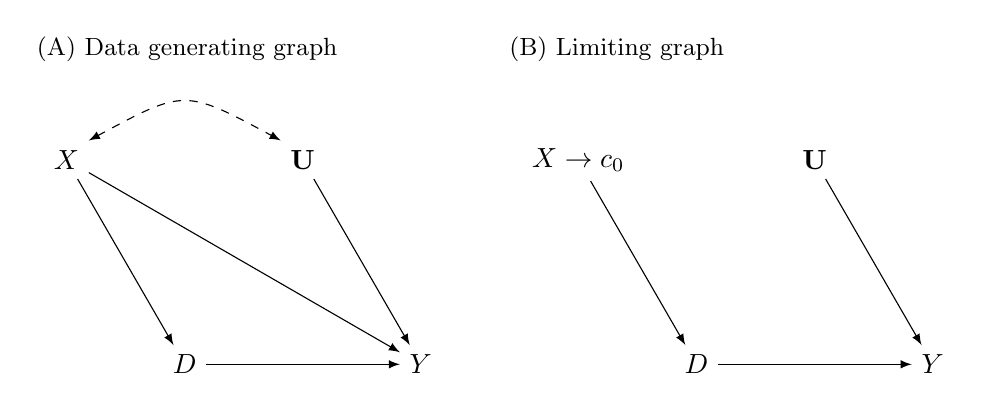
\begin{tikzpicture}
	% Figure A
\node (n1) at (0,2.598) {$X$};
\node (n2) at (1.5,0) {$D$};
\node (n3) at (3,2.598) {$\mathbf{U}$};
\node (n4) at (4.5,0) {$Y$};
\node [font=\small,anchor=west] at (-0.5,4) {(A) Data generating graph};
\draw [-{latex}] (n1) -- (n2);
\draw [-{latex}] (n1) -- (n4);
\draw [-{latex}] (n2) -- (n4);
\draw [-{latex}] (n3) -- (n4);
\draw [dashed, {latex}-{latex}] (n1.north east) .. controls (1.5,3.5) .. (n3.north west);
	
	% Figure B
	
\node (t1) at (6.5,2.598) {$X\to c_0$};
\node (t2) at (8,0) {$D$};
\node (t3) at (9.5,2.598) {$\mathbf{U}$};
\node (t4) at (11,0) {$Y$};
\node [font=\small,anchor=west] at (5.5,4) {(B) Limiting graph};
\draw [-{latex}] (t1) -- (t2);
\draw [-{latex}] (t2) -- (t4);
\draw [-{latex}] (t3) -- (t4);
	\end{tikzpicture}
\end{center}

\end{frame}

\begin{frame}[plain]
\begin{figure}
\centering
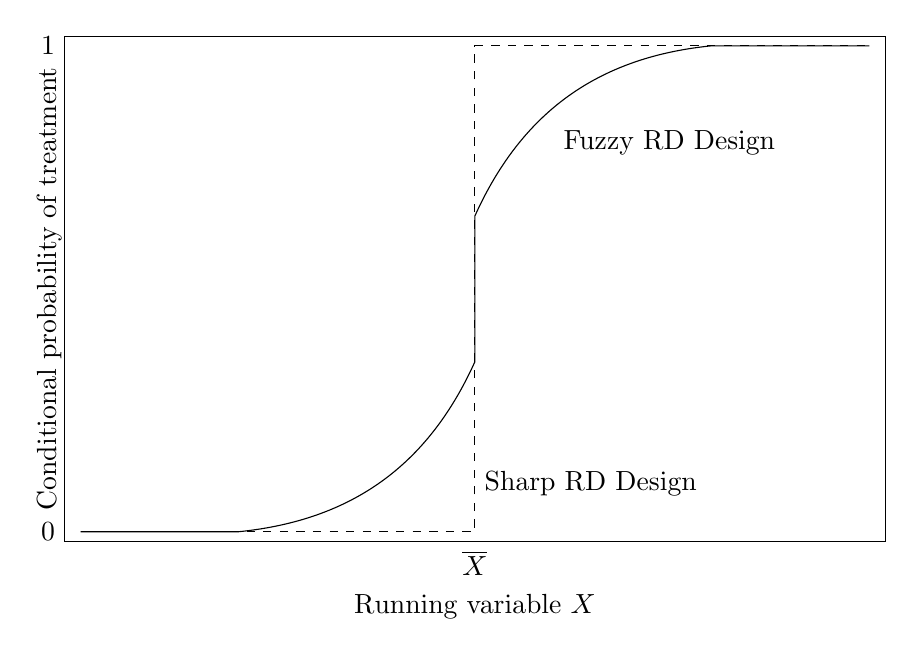
\begin{tikzpicture}
	\begin{axis}[
		xlabel={Running variable $X$},
		ylabel={Conditional probability of treatment},
		ylabel style={yshift=-0.5cm},
		ytick style={draw=none},
		xtick style={draw=none},
		width=12cm,
		height=8cm,
		xmin=-0.02,
		xmax=1.02,
		ymin=-0.02,
		ymax=1.02,
		xtick={0.5},
		xticklabel={$\overline{X}$},
		ytick={0,1}
	]
	
	\draw [dashed] (axis cs:0,0) -| (axis cs:0.5,1) -- (axis cs:1,1);
	\draw (axis cs:0,0) to 
				(axis cs:0.2,0) to 
				[bend right=30] (axis cs:0.5,0.35) to
				(axis cs:0.5,0.65) to
				[bend left=30] (axis cs:0.8,1) to
				(axis cs:1,1);
				
	\node [anchor=west] at (axis cs:0.5,0.1) {Sharp RD Design};
	\node [anchor=west] at (axis cs:0.6,0.8) {Fuzzy RD Design};
	
	\end{axis}
		
\end{tikzpicture}
\caption{Sharp vs. Fuzzy RDD}
\end{figure}

	

\end{frame}

\begin{frame}[plain]

	\begin{center}
	\textbf{Sharp vs. Fuzzy RDD}
	\end{center}
	
\begin{itemize}
\item There's traditionally thought to be two kinds of RD designs:
	\begin{enumerate}
	\item \underline{Sharp RDD}: Treatment is a deterministic function of running variable, $X$. Example: Medicare benefits.  
	\item \underline{Fuzzy RDD}: Discontinuous ``jump'' in the \emph{probability} of treatment when $X>c_0$.  Cutoff is used as an instrumental variable for treatment.  Example: attending state flagship
	\end{enumerate}
\item Fuzzy is a type of IV strategy and requires explicit IV estimators like 2SLS; sharp is reduced form IV and doesn't require IV-like estimators
\end{itemize}	

\end{frame}	

\begin{frame}[plain]
\begin{center}
\textbf{Overlap}
\end{center}

\begin{itemize}
\item Independence implies an equal distribution of characteristics across two groups guaranteeing overlap
	\begin{itemize}
	\item In an RCT you can find 65 year olds treated and untreated
	\end{itemize}
\item But RDD doesn't have this feature bc you don't have groups with the same value of $X$ in each group, so no overlap
	\begin{itemize}
	\item 64 years olds are control, not treatment. 66 years olds are in treatment not control
	\end{itemize}
\item Some methods require overlap and therefore are off the table without it; but RDD has a workaround using extrapolation
\end{itemize}

\end{frame}


\begin{frame}[plain]

	\begin{center}
	\textbf{Treatment assignment in the sharp RDD}
	\end{center}

		\begin{block}{Deterministic treatment assignment (``sharp RDD'')}
		In Sharp RDD, treatment status is a deterministic and discontinuous function of a covariate, $X_i$:  $$D_i =\begin{cases} 1 \text{ if }& X_i\geq{c_0} \\ 0 \text{ if } & X_i < c_0  \end{cases}$$where $c_0$ is a known threshold or cutoff.  In other words, if you know the value of $X_i$ for a unit $i$, you know treatment assignment for unit $i$ with certainty.  
		\end{block}
	
Universal health insurance: Americans aged 64 are not eligible for Medicare, but Americans aged 65 ($X\geq c_{65}$) are eligible for Medicare (ignoring disability exemptions)

%	\textcolor{blue}{Implication}: Sharp RDD relies on extrapolation across covariate values for its causal inference because there is no value of $X_i$ (e.g., age) for which you observe both treatment and control observations. Therefore, we cannot be agnostic about regression functional form as extrapolation depends on functional form.

\end{frame}	
	

\begin{frame}[plain]
	\begin{center}
	\textbf{Treatment effect definition and estimation}
	\end{center}
	
	\begin{block}{Definition of treatment effect}
	The treatment effect parameter, $\delta$, is the discontinuity in the conditional expectation function:
		\begin{eqnarray*}
		\delta&=&lim_{X_i\rightarrow{c_0}}E[Y^1_i|X_i=c_0] - lim_{c_0\leftarrow{X_i}}E[Y^0_i | X_i=c_0] \\
			&=&lim_{X_i\rightarrow{c_0}}E[Y_i|X_i=c_0] - lim_{c_0\leftarrow{X_i}}E[Y_i | X_i=c_0]
		\end{eqnarray*}The sharp RDD estimation is interpreted as an average causal effect of the treatment at the discontinuity$$\delta_{SRD}=E[Y^1_i - Y_i^0 | X_i=c_0]$$
	\end{block}
	$D$ is correlated with $X$ and deterministic function of $X$; overlap only occurs in the limit and thus the treatment effect is in the limit as $X$ approaches $c_0$
\end{frame}





\subsection{Smoothness, Extrapolation and Estimation}

\begin{frame}

	\begin{center}
	\textbf{Extrapolation}
	\end{center}
	
	\begin{itemize}
	\item In RDD, the counterfactuals are conditional on $X$.  
	\item We use \emph{extrapolation} in estimating treatment effects with the sharp RDD bc we do not have overlap
		\begin{itemize}
		\item Left of cutoff, only non-treated observations, $D_i=0$ for $X<c_0$
		\item Right of cutoff, only treated observations, $D_i=1$ for $X\geq c_0$
		\end{itemize}
	\item The extrapolation is to a counterfactual
	
	\end{itemize}

\end{frame}


\begin{frame}[plain]
\begin{center}
\textbf{Extrapolation}
\end{center}
Estimation methods attempt to approximate the limiting parameter using units left and right of the cutoff
	\begin{figure}
	\includegraphics[scale=0.2]{./lecture_includes/sim_extrapolation.png}
	\caption{Dashed lines are extrapolations}
	\end{figure}
\end{frame}




\subsubsection{Smoothness assumption}

\begin{frame}[plain]
	\begin{center}
	\textbf{Key identifying assumption}
	\end{center}
	
	\begin{block}{Smoothness (or continuity) of conditional expectation functions (Hahn, Todd and Van der Klaauw 2001)}
	$E[Y_i^0 | X=c_0]$ and $E[Y_i^1 | X=c_0]$ are continuous (smooth) in $X$ at $c_0$. 
	\end{block}
	
	\begin{itemize}
	\item Potential outcomes not actual outcomes
	\item If population average \emph{potential outcomes}, $Y^1$ and $Y^0$, are smooth functions of $X$ through the cutoff, $c_0$, then potential average outcomes \emph{won't} jump at $c_0$. 
	\item Implies the cutoff is exogenous -- i.e., nothing else changes related to potential outcomes at $c_0$
	\item Unobservables are evolving smoothly, too, through the cutoff
	\end{itemize}
	
\end{frame}


\begin{frame}[plain]
	\begin{center}
	\textbf{Smoothness is the identifying assumption and untestable}
	\end{center}
	

	\begin{itemize}
	\item The smoothness assumption allows us to use average outcome of units right below the cutoff as a valid counterfactual for units right above the cutoff. 
	\item In other words, extrapolation is allowed if smoothness is credible, and extrapolation is nonsensical if smoothing isn't credible
	\item The causal effect of the treatment will be based on \textbf{extrapolation} from the trend, $E[Y^0_i|X<c_0]$, to those values of $X>c_0$ for the $E[Y^0_i | X>c_0]$.  
	\item Means you have to think long and hard about smoothness and what violations mean in your context
	\item Why then is it not directly testable? Because potential outcomes are counterfactual
	\end{itemize}
	
\end{frame}



\begin{frame}[plain]
	\begin{center}
	\textbf{Graphical example of the smoothness assumption}
	\end{center}

\begin{figure}
\includegraphics[scale=0.3]{./lecture_includes/linear_ex_noe.png}
\end{figure}
Note these are \emph{potential} not \emph{actual} outcomes
\end{frame}


\begin{frame}[plain]
\begin{center}
\textbf{Graphical example of the treatment effect, not the smoothness assumption}
\end{center}

\begin{figure}
\includegraphics[scale=0.6]{./lecture_includes/linear_ex.pdf}
\end{figure}
Note that these are \emph{actual}, not \emph{potential} outcomes
\end{frame}


\begin{frame}[plain]

	\begin{center}
	\textbf{Re-centering the data}
	\end{center}
	
	\begin{itemize}
	\item It is common for authors to transform $X$ by ``centering'' at $c_0$:$$Y_i=\alpha + \beta(X_i-c_0) + \delta D_i +\varepsilon_i$$
	\item This doesn't change the interpretation of the treatment effect -- only the interpretation of the intercept.
%	\item Useful with interactions: $$Y=\alpha_0 + \alpha_1 Age + \alpha_2 Edu + \alpha_3 Age\times Edu$$ compared to$$
%	Y=\beta_0 + \beta_1(Age-65) + \beta_2 (Edu - 12) + \beta_3(Age - 65)\times(Edu-12)$$
	\end{itemize}

\end{frame}

\begin{frame}[plain]

\begin{center}
	\textbf{Re-centering the data}
\end{center}

\begin{itemize}
	\item Example: Medicare and age 65.  Center the running variable (age) by subtracting 65:
		\begin{eqnarray*}
		Y &=& \beta_0 + \beta_1(Age-65) + \beta_2 Edu \\
		&=& \beta_0 + \beta_1 Age - \beta_1 65 + \beta_2 Edu \\
		&=& \alpha + \beta_1 Age + \beta_2 Edu
		\end{eqnarray*}where $\alpha=\beta_0 - \beta_1 65$.  
		\item All other coefficients, notice, have the same interpretation, except for the intercept.
\end{itemize}

\end{frame}

\begin{frame}[plain]
\begin{center}
\textbf{Regression without re-centering}
\end{center}

\lstinputlisting{./lecture_includes/centering1.do} 

\end{frame}


\begin{frame}[plain]

	\begin{figure}
	\includegraphics[scale=0.15]{./lecture_includes/centering1.png}
	\end{figure}

\end{frame}


\begin{frame}[plain]
\begin{center}
\textbf{Regression with centering}
\end{center}

\lstinputlisting{./lecture_includes/centering2.do} 

\end{frame}

\begin{frame}[plain]

	\begin{figure}
	\includegraphics[scale=0.15]{./lecture_includes/centering2.png}
	\end{figure}

\end{frame}



\subsubsection{Nonlinearities}

\begin{frame}[plain]
	\begin{center}
	\textbf{Nonlinearity bias}
	\end{center}
	
	\begin{itemize}
	\item Smoothness and \emph{linearity} are different things.  
	\item What if the trend relation $E[Y_i^0 | X_i]$ does not jump at $c_0$ but rather is simply nonlinear?  
	\item Then your linear model will identify a treatment effect when there isn't because the functional form had poor predictive properties beyond the cutoff
	\item Let's look at a simulation
	\end{itemize}

\end{frame}

\begin{frame}[plain]

\lstinputlisting{./lecture_includes/centering3.do} 

\end{frame}

\begin{frame}[plain]
	
	\begin{figure}
	\includegraphics[scale=0.25]{./lecture_includes/bias_ex.png}
	\end{figure}

See how the two lines don't touch at $c_0$ but empirically should? That's bc the linear fit is the wrong functional form -- we know this from the simulation that it's the wrong functional form.
\end{frame}



\begin{frame}[plain]
	\begin{center}
	\textbf{Sharp RDD: Nonlinear Case}
	\end{center}
	
	\begin{itemize}
	\item Suppose the nonlinear relationship is $E[Y_i^0 | X_i]=f(X_i)$ for some reasonably smooth function $f(X_i)$ (drumroll -- like a cubic!) 
	\item In that case we'd fit the regression model:$$Y_i=f(X_i) + \delta{D_i} + \eta_i$$
	\item Since $f(X_i)$ is counterfactual for values of $X_i>c_0$, how will we model the nonlinearity? 
	\item There are 2 common ways of approximating $f(X_i)$	
	\end{itemize}
\end{frame}

\begin{frame}[plain]
\begin{center}
\textbf{Nonlinearities}
\end{center}

People until Gelman and Imbens 2018  favored``higher order polynomials'' but this is problematic due to overfitting. Gelman and Imbens 2018 recommend at best a quadratic
		\begin{enumerate}
		\item Use global and local regressions with $f(X_i)$ equalling a $p^{th}$ order polynomial 
		\begin{eqnarray*}
		Y_i&=&\alpha +\delta{D_i}  +  \beta_1x_i + \beta_2x_i^2 + \dots + \beta_px_i^p + \eta_i
		\end{eqnarray*}
		\item Or use some nonparametric kernel method which I'll cover later
		\end{enumerate}

\end{frame}

\begin{frame}[plain]
	\begin{center}
	\textbf{Different polynomials on the 2 sides of the discontinuity}
	\end{center}
	
	\begin{itemize}
	\item We can generalize the function, $f(x_i)$, by allowing it to differ on both sides of the cutoff by including them both individually and interacting them with $D_i$.  
	\item In that case we have:
		\begin{eqnarray*}
		E[Y_i^0 | X_i] &=& \alpha + \beta_{01}\tilde{X}_i + \beta_{02}\tilde{X}_i^2 + \dots + \beta_{0p}\tilde{X}_i^p \\
		E[Y_i^1 | X_i] &=& \alpha + \delta + \beta_{11}\tilde{X}_i + \beta_{12}\tilde{X}_i^2 + \dots + \beta_{1p}\tilde{X}_i^p
		\end{eqnarray*}where $\tilde{X}_i$ is the centered running variable (i.e., $X_i - c_0$). 
		
	\end{itemize}
\end{frame}


\begin{frame}[plain]
\begin{center}
\textbf{Lines to the left, lines to the right of the cutoff}
\end{center}

\begin{itemize}
		\item Re-centering at $c_0$ ensures that the treatment effect at $X_i=c_0$ is the coefficient on $D_i$ in a regression model with interaction terms
		\item As Lee and Lemieux (2010) note, allowing different functions on both sides of the discontinuity should be the main results in an RDD paper 
\end{itemize}

\end{frame}

\begin{frame}[plain]
	\begin{center}
	\textbf{Different polynomials on the 2 sides of the discontinuity}
	\end{center}
	
	\begin{itemize}
	\item To derive a regression model, first note that the observed values must be used in place of the potential outcomes:$$E[Y | X] = E[Y^0 | X] + \left (E[Y^1 | X] - E[Y^0 | X] \right)D$$which is the switching equation from earlier expressed in terms of conditional expectation functions
	\item Regression model you estimate is:
		\begin{eqnarray*}
		Y_i &=& \alpha + \beta_{01}\tilde{x}_i + \beta_{02}\tilde{x}_i^2 + \dots + \beta_{0p}\tilde{x}_i^p \\
		& & + \delta{D}_i + \beta_1^*D_i\tilde{x}_i + \beta_2^*D_i\tilde{x}_i^2 + \dots + \beta_p^*D_i\tilde{x}_i^p + \varepsilon_i 
		\end{eqnarray*}where $\beta^*_1 = \beta_{11} - \beta_{01}$, $\beta_2^* = \beta_{21} - \beta_{21}$ and $\beta_p^*=\beta_{1p}-\beta_{0p}$
	\item The treatment effect at $c_0$ is $\delta$
	\end{itemize}
\end{frame}


\begin{frame}[plain]
	\begin{center}
	\textbf{Polynomial simulation example}
	\end{center}

\lstinputlisting{./lecture_includes/poly1.do} 
	
\end{frame}


\begin{frame}[plain]
	\begin{center}
	\textbf{Polynomial simulation example}
	\end{center}

\begin{figure}
\includegraphics[scale=0.55]{./lecture_includes/more_flex.pdf}
\caption{Third degree polynomial. Actual model second degree polynomial.}
\end{figure}

Notice: no more gap at $c_0$ once we model the function $f(x)$
\end{frame}

\begin{frame}[plain]
\begin{center}
\textbf{Stata simulation}
\end{center}


\lstinputlisting{./lecture_includes/rdd5.do} 

\end{frame}


\begin{frame}[plain]
	\begin{center}
	\textbf{Polynomial simulation example}
	\end{center}

\begin{figure}
\includegraphics[scale=0.2]{./lecture_includes/poly6.png}
\end{figure}

Notice: no more gap at $c_0$ once we model the function $f(x)$ (e.g., $D$ is insignificant once we include polynomials)
\end{frame}

\begin{frame}[plain]
	\begin{center}
	\textbf{Polynomial simulation example}
	\end{center}

\begin{figure}
\includegraphics[scale=0.2]{./lecture_includes/poly4.png}
\end{figure}

And centering did nothing to the interpretation of the main results ($D$), only to the intercept.

\end{frame}



\subsection{Testing for violations}

\begin{frame}
\begin{center}
\textbf{Robustness against what?}
\end{center}

\begin{itemize}
\item Are you done now that you have your main results? No
\item You main results are only causal insofar as smoothness is a credible belief, and since smoothness isn't guaranteed by ``the science'' like an RCT, you have to build your case
\item You must now scrutinize alternative hypotheses that are consistent with your main results through sensitivity checks, placebos and alternative approaches
\end{itemize}

\end{frame}

\begin{frame}[plain]
\begin{center}
\textbf{Main Challenges}
\end{center}

Classify your concern regarding smoothness violations into two categories:
\begin{itemize}
\item Manipulation on the running variable 
\item Endogeneity of the cutoff
\end{itemize}Most robustness is aimed at building credibility around these, 

\end{frame}




\begin{frame}[plain]

	\begin{center}
	\textbf{Manipulation of your running variable score}
	\end{center}
	
	\begin{itemize}
	\item Treatment is not as good as randomly assigned around the cutoff, $c_0$, when agents are able to manipulate their running variable scores.  This happens when:
		\begin{enumerate}
		\item the assignment rule is known in advance
		\item agents are interested in adjusting
		\item agents have time to adjust
		\item administrative quirks like nonrandom heaping along the running variable
		\end{enumerate}
Examples include re-taking an exam, self-reported income, certain types of non-random rounding.
	\item Since necessarily treatment assignment is no longer independent of potential outcomes, it's likely this implies smoothness has been violated
	\end{itemize}
\end{frame}



\begin{frame}[plain]
	\begin{center}
	\textbf{Test 1: Manipulation of the running variable}
	\end{center}
	
	\begin{block}{Manipulation of the running variable}
Assume a desirable treatment, $D$, and an assignment rule $X\geq{c_0}$.  If individuals sort into $D$ by choosing $X$ such that $X\geq{c_0}$, then we say individuals are manipulating the running variable. 
	\end{block}
Also can be called ``sorting on the running variable'' -- same thing

\end{frame}

\begin{frame}[plain]
\begin{center}
\textbf{A badly designed RCT}
\end{center}

	\begin{itemize}
		\item Suppose a doctor randomly assigns heart patients to statin and placebo to study the effect of the statin on heart attacks within 10 years 
		\item Patients are placed in two different waiting rooms, $A$ and $B$, and plans to give those in $A$ the statin and those in $B$ the placebo. 
		\item The doors are unlocked and movement between the two can happen
		\item Versions of this happened with HIV RCTs in the 1980s ironically in which medication from treatment group was given to the control group, but I'm talking about something a little different
	\end{itemize}

\end{frame}

\begin{frame}[plain]
	\begin{center}
	\textbf{McCrary Density Test}
	\end{center}

We would expect waiting room $A$ to become \emph{crowded}. In the RDD context, sorting on the running variable implies heaping on the ``good side'' of $c_0$
	\begin{itemize}
	\item McCrary (2008) suggests a formal test: under the null the \emph{density} should be continuous at the cutoff point. 
	\item Under the alternative hypothesis, the density should increase at the kink (where $D$ is viewed as good) 
		\begin{enumerate}
		\item Partition the assignment variable into bins and calculate frequencies (i.e., number of observations) in each bin
		\item Treat those frequency counts as dependent variable in a local linear regression
		\end{enumerate}
	\item This is oftentimes visualized with confidence intervals illustrating the effect of the discontinuity on density - you need no jump to pass this test
	\end{itemize}
	
\end{frame}

\begin{frame}[plain]
\begin{center}
\textbf{McCrary density test}
\end{center}

\begin{itemize}
	\item The McCrary Density Test has become \textbf{mandatory} for every analysis using RDD. 
		\begin{itemize}
		\item If you can estimate the conditional expectations, you evidently have data on the running variable. So in principle you can always do a density test
		\item You can download the (no longer supported) Stata ado package, \texttt{DCdensity}, to implement McCrary's density test (\url{http://eml.berkeley.edu/~jmccrary/DCdensity/})
		\item You can install \texttt{rdrobust} for Stata and R too, and it will implement the test
		\end{itemize}
\end{itemize}

\end{frame}

\begin{frame}[shrink=20,plain]
	\begin{center}
	\textbf{Caveats about McCrary Density Test}
	\end{center}
	
	\begin{itemize}
		\item For RDD to be useful, you already need to know something about the mechanism generating the assignment variable and how susceptible it could be to manipulation. Note the rationality of economic actors that this test is built on.
		\item A discontinuity in the density is ``suspicious'' -- it \emph{suggests} manipulation of $X$ around the cutoff is probably going on. In principle one doesn't need continuity.  
		\item This is a high-powered test. You need a lot of observations at $c_0$ to distinguish a discontinuity in the density from noise.  
	\end{itemize}

	\begin{figure}
	\includegraphics[scale=0.75]{./lecture_includes/mccrary_density_test.pdf}
	\caption{\scriptsize Panel C is density of income when there is no pre-announcement and no manipulation. Panel D is the density of income when there is pre-announcement and manipulation. From McCrary (2008).}
	\end{figure}

\end{frame}


\begin{frame}[shrink=20,plain]
	\begin{center}
	\textbf{Visualizing manipulation}
	\end{center}
 
        \begin{center}
		\begin{figure}
		\begin{columns}
		
		\column{.45\textwidth}
		\includegraphics[scale=0.4]{./lecture_includes/marathon_heaping.pdf}
		\column{.45\textwidth}
		\includegraphics[scale=0.4]{./lecture_includes/marathon_mccrary_tests.pdf}

		\end{columns}
		\caption{\scriptsize Figures 2 and 3 from Eric Allen, Patricia Dechow, Devin Pope and George Wu's (2013) ``Reference-Dependent Preferences: Evidence from Marathon Runners''. \url{http://faculty.chicagobooth.edu/devin.pope/research/pdf/Website_Marathons.pdf} }
		\end{figure}
        \end{center}
\end{frame}

\begin{frame}[plain]
\begin{center}
\textbf{Newborn mortality and medical expenditure}
\end{center}

\begin{itemize}
\item Almond, et al. 2010 attempted to estimate the causal effect of medical expenditures on health outcomes, which is ordinarily rife with selection bias due to endogeneous physician behavior (independence is violated)
\item In the US, newborns whose birthweight falls below 1500 grams receive heightened medical attention bc 1500 is the ``very low birth weight'' range and quite dangerous for infants
\item Used RDD with hospital administrative records and found 1-year infant mortality decreased by 1pp just below 1500 grams compared to just above -- medical expenditures are cost-effective
\end{itemize}

\end{frame}


\begin{frame}[plain]
\begin{center}
\textbf{Heaping problem}
\end{center}


\begin{figure}[htb]
\centering	\includegraphics[scale=0.08]{./lecture_includes/heaping.jpg}%.jpg}
\caption{Distribution of births by gram from Almond, et al. 2010}
\end{figure}

\end{frame}

\begin{frame}[plain]
\begin{center}
\textbf{Heaping, Running and Jumping}
\end{center}

\begin{itemize}
\item This picture shows ``heaping'' which is excess mass at certain points along the running variable
\item Unlikely births actually heap at certain intervals; more likely someone is rounding
\item Some scales may be less sophisticated, some practices may be more common in some types of hospitals than others, there could outright manipulation
\end{itemize}

\end{frame}

\begin{frame}[plain]
\begin{center}
\textbf{Failure to reject}
\end{center}

\begin{itemize}
\item Almond, et al. 2010 used the McCrary density test but found no evidence of manipulation
\item Ironically, the McCrary density test may fail to reject in a heaping scenario
\item In this scenario, the heaping is associated with high mortality children who are outliers compared to newborns both to the left and to the right
\end{itemize}

\end{frame}

\begin{frame}[plain]

\begin{quote}
``This [heaping at 1500 grams] may be a signal that poor-quality hospitals have relatively high propensities to round birth weights but is also consistent with manipulation of recorded birth weights by doctors, nurses, or parents to obtain favorable treatment for their children. Barreca, et al. 2011 show that this nonrandom heaping leads one to conclude that it is ``good'' to be strictly less than any 100-g cutoff between 1,000 and 3,000 grams.''
\end{quote}

\end{frame}

\begin{frame}[plain]
\begin{center}
\textbf{Donut holes}
\end{center}

\begin{itemize}
\item RDD compares means as we approach $c_0$ from either direction along $X$
\item Estimates should not logically be sensitive to the observations at the cutoff -- if it is, then smoothness may be violated
\item Through Monte Carlos, Barreca, et al. 2016 suggest an alternative strategy -- drop the units in the vicinity of 1500 grams, and re-estimate the model
\item They call this a ``donut'' RDD bc you drop the units at the cutoff (the ``donut hole'') and estimate your model on the units in the neighborhood instead
\end{itemize}

\end{frame}

\begin{frame}[plain]
\begin{center}
\textbf{Newborn mortality and medical expenditure}
\end{center}

\begin{itemize}
\item Dropping units (e.g., trimming) always changes the parameter we're estimating -- it's not the ATE, the ATT, not even the LATE except under strong assumptions
\item In this case, dropping at the threshold reduced sample size by 2\%
\item But the strength of this practice is that it allows for the possibility that units at the heap differ markedly due to selection bias than those in the surrounding area
\item Donut RDD analysis found effect sizes that were approximately 50\% smaller than Almond, et al 2010
\item Caution with heaping is a good attitude to have
\end{itemize}

\end{frame}





\begin{frame}[plain]
\begin{center}
\textbf{Endogenous cutoffs}
\end{center}

\begin{center}
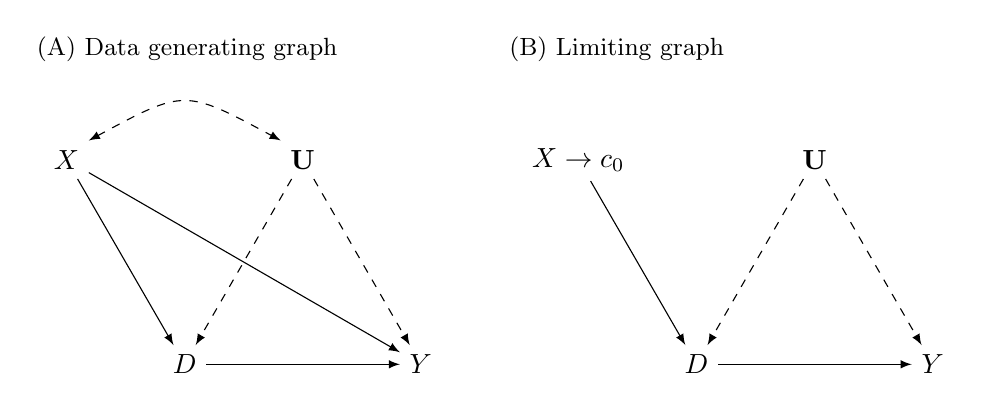
\begin{tikzpicture}
	% Figure A
\node (n1) at (0,2.598) {$X$};
\node (n2) at (1.5,0) {$D$};
\node (n3) at (3,2.598) {$\mathbf{U}$};
\node (n4) at (4.5,0) {$Y$};
\node [font=\small,anchor=west] at (-0.5,4) {(A) Data generating graph};
\draw [-{latex}] (n1) -- (n2);
\draw [-{latex}] (n1) -- (n4);
\draw [-{latex}] (n2) -- (n4);
\draw [dashed, -{latex}] (n3) -- (n4);
\draw [dashed, -{latex}] (n3) -- (n2);
\draw [dashed, {latex}-{latex}] (n1.north east) .. controls (1.5,3.5) .. (n3.north west);
	
	% Figure B
	
\node (t1) at (6.5,2.598) {$X\to c_0$};
\node (t2) at (8,0) {$D$};
\node (t3) at (9.5,2.598) {$\mathbf{U}$};
\node (t4) at (11,0) {$Y$};
\node [font=\small,anchor=west] at (5.5,4) {(B) Limiting graph};
\draw [-{latex}] (t1) -- (t2);
\draw [-{latex}] (t2) -- (t4);
\draw [dashed, -{latex}] (t3) -- (t4);
\draw [dashed, -{latex}] (t3) -- (t2);
	\end{tikzpicture}
\end{center}

\end{frame}



\begin{frame}[plain]

\begin{center}
\textbf{Endogeneous cutoffs}
\end{center}

\begin{itemize}

	\item RCT randomization breaks all ordinary backdoor paths between $D$ and $Y$ because that's how ``the science'' of randomization works
	\item RDD blocks the backdoor path from $D \leftarrow X \leftarrow ? \rightarrow U \rightarrow Y$; it \emph{assumes} away the backdoor path $D \leftarrow U \rightarrow Y$
	\item But if cutoffs are endogenous, then it is there, which means absent the treatment, smoothness would've been violated \emph{anyway}
	\item Smoothness isn't guaranteed by an RDD unless $D \leftarrow U \rightarrow Y$ isn't present -- which is why it is \emph{the} critical identifying assumption
	
\end{itemize}

\end{frame}


\begin{frame}[plain]
\begin{center}
\textbf{Endogeneous cutoffs}
\end{center}

\begin{itemize}
\item Examples of endogenous cutoffs
	\begin{itemize}
	\item Age thresholds used for policy (i.e., person turns 18, and faces more severe penalties for crime) is correlated with other variables that affect the outcome (i.e., graduation, voting rights, etc.)
	\item Age 65 is correlated with factors that directly affect healthcare expenditure and mortality such as retirement
	\end{itemize}
\item But some of these can be weakly defended with balance tests (observables), or may be directly testable through placebos assuming you have the data
\end{itemize}

\end{frame}
	
	
\begin{frame}[plain]
	\begin{center}
	\textbf{Evaluating smoothness through balance}
	\end{center}
	
	\begin{itemize}
	\item Balance tests and placebo tests are related but distinct
	\item We can't directly test smoothness bc we are missing counterfactuals
	\item Ask yourself: why should average values of exogenous covariates jump if potential outcomes are smooth through the cutoff?
	\item If there are exogenous (non collider) covariates strongly associated with potential outcomes but exogenous to them, then they should be the same on either side of the cutoff if smoothness holds
	\item In this sense, balance tests are indirect searching for evidence supporting smoothness
	\end{itemize}
\end{frame}

\begin{frame}[plain]
\begin{center}
\textbf{Balance implementation}
\end{center}


Don't make it hard -- do what you did to $Y$, only to $Z$
		\begin{itemize}
		\item Choose other noncolliders associated with potential outcomes, $Z$ 
		\item Create similar graphical plots as you did for $Y$
		\item Could also conduct the parametric and nonparametric estimation on $Z$
		\item You do \textbf{not} want to see a jump around the cutoff, $c_0$
		\end{itemize}

\end{frame}

\begin{frame}[shrink=20,plain]
	\begin{center}
	\textbf{Visualizing Balance}
	\end{center}
	
	\begin{figure}
	\includegraphics[scale=0.85]{./lecture_includes/lee_moretti_butler_fig3.pdf}
	\caption{\scriptsize Figure 3 from Lee, Moretti and Butler (2004), ``Do Voters Affect or Elect Policies?'' \emph{Quarterly Journal of Economcis}. Panels refer to (top left to bottom right) the following district characteristics: real income, percentage with high-school degree, percentage black, percentage eligible to vote. Circles represent the average characteristic within intervals of 0.01 in Democratic vote share. The continuous line represents the predicted values from a fourth-order polynomial in vote share fitted separately for points above and below the 50 percent threshold. The dotted line represents the 95 percent confidence interval.}
	\end{figure}
	
\end{frame}

\begin{frame}[plain]
	\begin{center}
	\textbf{Placebos at non-discontinuous points}
	\end{center}
	
	\begin{itemize}
	\item Placebos in time are common with panels; placebo in running variables are their equivalent in RDD
	\item Imbens and Lemieux (2010) suggest we look at one side of the discontinuity (e.g., $X<c_0$), take the median value of the running variable in that section, and pretend it was a discontinuity, $c_0'$
	\item Then test whether in reality there is a discontinuity at $c_0'$.   You do \textbf{not} want to find anything.
	\item Remember though: smoothness at placebo points is neither necessary nor sufficient for smoothness in the potential outcomes at the cutoff
	\item So there are Type I and Type II risks of error with this
	\end{itemize}
\end{frame}

\subsection{Visualization}


\begin{frame}

\begin{center}
\textbf{Pictures, pictures and more pictures}
\end{center}

\begin{itemize}
\item Synthetic control and RDD are visually intense
\item Eyeball tests are rampant (and deservedly) in RDD studies
\item Even if your main results are all parametric, you'll still want to present at least some nonparametric style pictures according to Imbens and Lemieux (2010)
\item Let's review some of the graphs you have to include 
\end{itemize}

\end{frame}	

\begin{frame}[plain]
	\begin{center}
	\textbf{Outcomes}
	\end{center}
	
	\begin{enumerate}
	\item \textbf{Outcome by running variable, $(X_i)$:}
		\begin{itemize}
		\item Construct bins and average the outcome within bins on both sides of the cutoff
		\item Look at different bin sizes when constructing these graphs 
		\item Plot the running variables, $X_i$, on the horizontal axis and the average of $Y_i$ for each bin on the vertical axis
		\item Consider plotting a relatively flexible regression line on top of the bin means, but some readers prefer an eyeball test without the regression line to avoid ``priming''
		\end{itemize}
	\end{enumerate}
\end{frame}

\begin{frame}[shrink=20,plain]
	\begin{center}
	\textbf{Example: Outcomes by Running Variables}
	\end{center}
	
	\begin{figure}
	\includegraphics[scale=1.05]{./lecture_includes/rdd_30.pdf}
	\end{figure}
	
\end{frame}


\begin{frame}[shrink=20,plain]
	\begin{center}
	\textbf{Example: Outcomes by Running Variables with smaller bins}
	\end{center}
	
	\begin{figure}
	\includegraphics[scale=1.05]{./lecture_includes/rdd_31.pdf}
	\end{figure}
	
\end{frame}

\begin{frame}[plain]
	\begin{center}
	\textbf{Probability of treatment}
	\end{center}
	
	\begin{enumerate}\addtocounter{enumi}{1}
	\item \textbf{Probability of treatment by running variable if fuzzy RDD}
		\begin{itemize}
		\item In a fuzzy RDD, you also want to see that the treatment variable jumps at $c_0$ 
		\item This tells you whether you have a first stage (``bite'')
		\item Let's look at that again from earlier Hoekstra (2008) and enrollment at the flagship
		\end{itemize}
	\end{enumerate}
\end{frame}

\begin{frame}[plain]

			\begin{figure}
  \makebox[\textwidth][c]{\includegraphics[width=1\textwidth]{./lecture_includes/rdd_hoekstra1}}%
	\end{figure}

\end{frame}

\begin{frame}[plain]
	\begin{center}
	\textbf{McCrary Density}
	\end{center}
	
	\begin{enumerate}\addtocounter{enumi}{2}
	\item \textbf{Density of the running variable}
		\begin{itemize}
		\item One should plot the number of observations in each bin.
		\item This plot allows to investigate whether there is a discontinuity or heaping in the distribution of the running variable at the threshold
		\item Heaping or discontinuities in the density suggest that people can manipulate their running variable score
		\item This is an indirect test of the identifying assumption that each individual has imprecise control over the assignment variable, which may violate smoothness
		\end{itemize}
	\end{enumerate}
\end{frame}


\begin{frame}[plain]
	\begin{center}
	\textbf{Density of the running variable}
	\end{center}
	
	\begin{figure}
	\includegraphics[scale=0.75]{./lecture_includes/rdd_33.pdf}
	\end{figure}
	
\end{frame}

\begin{frame}[plain]
\begin{center}
\textbf{Balance pictures}
\end{center}

\begin{enumerate}\addtocounter{enumi}{3}
	\item \textbf{Covariates by a running variable}
		\begin{itemize}
		\item Construct a similar graph to the outcomes graph but use a noncollider covariate as the ``outcome''
		\item Balance implies smoothness through the cutoff, $c_0$.  
		\item If noncollider covariates jump at the cutoff, one is probably justified to reject that potential outcomes aren't also probably jumping there
		\end{itemize}
	\end{enumerate}
\end{frame}




\begin{frame}[plain]
	\begin{center}
	\textbf{Example: Covariates by Running Variable}
	\end{center}
	
	\begin{figure}
	\includegraphics[scale=0.75]{./lecture_includes/rdd_32.pdf}
	\end{figure}
	
\end{frame}



\subsection{Inference, kernels, bandwidths}

\begin{frame}
\begin{center}
\textbf{Inference -- honesty}
\end{center}

\begin{itemize}
\item Lee and Card (2008) and Lee and Lemieux (2010) recommend clustering standard errors on the running variable 
\item Koles\'ar and Rothe (2018) provide extensive theoretical and simulation-based evidence that this is not good; you'd be better off just with heteroskedastic robust
\item They propose two alternative confidence intervals that achieve correct coverage in large samples -- called ``honest'' (great intro! Still studying this procedure)
\item Unavailable in Stata, but is available in R -- RDHonest -- at \url{https://github.com/kolesarm/RDHonest}
\end{itemize}

\end{frame}

\begin{frame}[plain]
\begin{center}
\textbf{Inference -- randomization inference}
\end{center}

\begin{itemize}
\item Cattaeneo, et al. (2015) say to consider that the cutoff is a randomized experiment
\item Use randomization inference which is a test of the null of no individual unit level treatment effect at the cutoff
\end{itemize}

\end{frame}



\begin{frame}[plain]
\begin{center}
\textbf{Parametric vs. nonparametric approaches}
\end{center}

\begin{itemize}
\item Least squares approaches, because it models the counterfactual using functional forms, is parametric 
\item As a result, it can have poor predictive properties on counterfactuals above/below the cutoff
\item Another way of approximating $f(X_i)$ is to use a nonparametric kernel which has its own problems; just not that one.
\end{itemize}

\end{frame}



\begin{frame}[plain]
	\begin{center}
	\textbf{Kernel regression}
	\end{center}
	
		\begin{figure}
		\includegraphics[scale=1.2]{./lecture_includes/kernel_1.pdf}
		\end{figure}
	\begin{itemize}

	\item While the ``true'' effect is $AB$, with a certain bandwidth a rectangular kernel would estimate the effect as $A'B'$
	\item There is therefore systematic bias with the kernel method if the $f(X)$ is upwards or downwards sloping
	\end{itemize}
\end{frame}


\begin{frame}[plain]
	\begin{center}
	\textbf{Kernel weighted local polynomial regression}
	\end{center}
	
	\begin{itemize}
	\item The nonparametric one-sided kernel estimation problems are called ``boundary problems'' at the cutoff (Hahn, Todd and Van der Klaauw 2001)
	\item Kernel estimation (such as lowess) may have poor properties because the point of interest is at a boundary 
	\item They proposed to use ``local linear nonparametric regressions'' instead
	\end{itemize}
	
\end{frame}




\begin{frame}[plain]
	\begin{center}
	\textbf{Local linear regression with weights}
	\end{center}
	
	\begin{itemize}
	\item Local linear nonparametric regression substantially reduces the bias
	\item Think of it as a weighted regression restricted to a window -- kernel provides the weights to that regression.  
	\end{itemize}\begin{eqnarray*}
	(\widehat{a}, \widehat{b}) \equiv_{a,b} \sum_{i=1}^n (y_i - a - b(x_i-c_0))^2 K\bigg ( \frac{x_i - c_0}{h} \bigg ) 1(x_i > c_0)
	\end{eqnarray*}where $x_i$ is the value of the running variable, $c_0$ is the cutoff, $K$ is a kernel function and $h>0$ is a suitable bandwidth
\end{frame}

\begin{frame}[plain]
\begin{center}
\textbf{Animation of a local linear regression}
\end{center}

\url{https://twitter.com/page_eco/status/958687180104245248}

\end{frame}

\begin{frame}[plain]
\begin{center}
\textbf{Estimation}
\end{center}

\begin{itemize}
	\item Stata's \texttt{poly} estimates kernel-weighted local polynomial regressions.  
	\item A rectangular kernel would give the same result as $E[Y]$ at a given bin on $X$.  The triangular kernel gives more importance to observations close to the center.
	\item This method will be sensitive to how large the bandwidth (window) you choose
\end{itemize}

\end{frame}




\begin{frame}[plain]
	\begin{center}
	\textbf{Optimal bandwidths}
	\end{center}
	
	\begin{itemize}
	\item A rectangular kernel would give the same result as taking $E[Y]$ at a given bin on $X$ whereas the triangular kernel gives more importance to the observations closer to the center. 
	\item While estimating this in a given window of width $h$ around the cutoff is straightforward, it's more difficult to choose this bandwidth (or window), and the method is sensitive to the choice of bandwidth. 
	\end{itemize}
	
\end{frame}



\begin{frame}[plain]
\begin{center}
\textbf{Bandwidths}
\end{center}

\begin{itemize}
\item Several methods for choosing the optimal bandwidth (window), but it's always a trade off between bias and variance
\item In practical applications, you want to check for balance around that window
\item Standard error of the treatment effects can be bootstrapped but there are also other alternatives
\item You could add other variables to nonparametric methods.
\end{itemize}

\end{frame}

\begin{frame}[plain]
\begin{center}
\textbf{Bandwidths}
\end{center}

\begin{itemize}
\item Imbens and Kalyanaraman (2012), and more recently Calonico, et al. (2017), have proposed methods for estimating ``optimal'' bandwidths which may differ on either side of the cutoff. 
\item Calonico, et al (2017) propose local-polynomial regression discontinuity estimators with robust confidence intervals
\item Stata ado package and R package are both called \texttt{rdrobust}
\end{itemize}

\end{frame}




\subsection{Sub-RDD: Close election designs}

\begin{frame}

	\begin{figure}
	\includegraphics[scale=0.15]{./lecture_includes/lmb_qje.png}
	\end{figure}

\end{frame}


		
\begin{frame}[plain]
\begin{center}
\textbf{Implementation}
\end{center}

\begin{itemize}
\item The following paper is a seminal paper in public choice both scientifically and methodologically -- the close election RDD
\item I call the close election RDD a type of sub-RDD in that it's widely used in political science and economics to the point that it's taken on a life of its own
\item Let's take everything we've done and apply it by replicating this paper using programs I've provided
\end{itemize}

\end{frame}


\begin{frame}[plain]
\begin{center}
\textbf{Public choice}
\end{center}

There are two fundamentally different views of the role of voters in a representative democracy.
		\begin{enumerate}
		\item \textbf{Convergence}: Voters force candidates to become relatively moderate depending on their size in the distribution (Downs 1957).  \begin{quote}``Competition for votes can force even the most partisan Republicans and Democrats to moderate their policy choices. In the extreme case, competition may be so strong that it leads to `full policy convergence': opposing parties are forced to adopt identical policies'' -- Lee, Moretti, and Butler 2004.\end{quote}
		\item \textbf{Divergence}: Voters pick the official and after taking office, she pursues her most-preferred policy.  
		\end{enumerate}

\end{frame}


\begin{frame}[plain]
\begin{center}
\textbf{Falsification of either hypothesis had been hard}
\end{center}

\begin{itemize}
\item Very difficult to test either one of these since you don't observe the counterfactual votes of the loser for the same district/time
\item Winners in a district are selected based on their policy's conforming to unobserved voter preferences, too
\item Lee, Moretti and Butler (2004) develop the ``close election RDD'' which has the aim of determining whether convergence, while theoretically appealing, has any explanatory power in Congress
\item The metaphor of the RCT is useful here: maybe close elections are being determined by coin flips (e.g., a few votes here, a few votes there)
\end{itemize}

\end{frame}






\begin{frame}[plain]
	\begin{center}
	\textbf{Outcome is Congress person's liberal voting score}
	\end{center}
	
	\begin{itemize}
	\item \textbf{Liberal voting score} is a report card from the Americans for Democratic Action (ADA) for the House election results 1946-1995
		\begin{itemize}
		\item Authors use the ADA score for all US House Representatives from 1946 to 1995 as their voting record index
		\item For each Congress, ADA chooses about twenty high-profile roll-call votes and creates an index varying 0 and 100 for each Representative of the House measuring liberal voting record
		\end{itemize}
	\end{itemize}
\end{frame}

\begin{frame}[plain]
\begin{center}
\textbf{Democratic ``voteshare'' is the running variable}
\end{center}

\begin{itemize}
	\item \textbf{Voteshare} from the same races
		\begin{itemize}
		\item The running variable is \texttt{voteshare} which is the share of all votes that went to a Democrat. 
		\item They use a close Democratic victory to check whether convergence or divergence is correct (what's smoothness here?)
		\item  Discontinuity in the running variable occurs at \texttt{voteshare}$=0.5$. When \texttt{voteshare}$>0.5$, the Democratic candidate wins.  
		\end{itemize}
	\item I'll show \texttt{lmb1.do} to \texttt{lmb10.do} (and R) at times just so we can all see the simple estimation methods ourselves. 
\end{itemize}

\end{frame}

\begin{frame}[plain]
	\begin{center}
	\textbf{Remember these results}
	\end{center}
	
	\begin{figure}
	\includegraphics[scale=0.75]{./lecture_includes/lee_table1.pdf}
	\caption{Lee, Moretti, and Butler 2004, Table 1.}
	\end{figure}
\end{frame}


\clearpage
\newpage

	
\begin{frame}[plain]
	\begin{center}
	\textbf{Nonparametric estimation}
	\end{center}
	
	\begin{itemize}
	\item Hahn, Todd and Van der Klaauw (2001) emphasized using local polynomial regressions
	\item Estimate $E[Y|X]$ in such a way that doesn't require committing to a functional form 
	\item That model would be something general like$$Y=f(X) + \varepsilon$$
	\end{itemize}
\end{frame}

\begin{frame}[plain]
\begin{center}
\textbf{Nonparametric estimation (cont.)}
\end{center}

\begin{itemize}
	\item We'll do this estimation just rolling $E[ ADA ]$ across the running variable $voteshare$ visually
	\item Stata has an option to do this called \texttt{cmogram} and it has a lot of useful options, though many people prefer to graph it themselves bc it gives more flexibility.  
	\item We can recreate Figures I, IIA and IIB using it
\end{itemize}
\end{frame}
	


\begin{frame}[plain]
	\begin{center}
	\textbf{Future liberal voting score}
	\end{center}
	
	\begin{figure}
	\includegraphics[scale=0.6]{./lecture_includes/lee_fig1.pdf}
	\caption{Lee, Moretti, and Butler 2004, Figure I. $\gamma\approx 20$}
	\end{figure}
\end{frame}

\clearpage
\newpage

\begin{frame}[plain]
	\begin{center}
	\textbf{Contemporaneous liberal voting score}
	\end{center}
	
	\begin{figure}
	\includegraphics[scale=0.75]{./lecture_includes/lee_fig2.pdf}
	\caption{Lee, Moretti, and Butler 2004, Figure IIa. $\pi_1\approx 45$}
	\end{figure}
\end{frame}


\begin{frame}[plain]
	\begin{center}
	\textbf{Incumbency advantage}
	\end{center}
	
	\begin{figure}
	\includegraphics[scale=0.75]{./lecture_includes/lee_fig2b.pdf}
	\caption{Lee, Moretti, and Butler 2004, Figure IIb. $(P_{t+1}^D - P_{t+1}^R)\approx 0.50$}
	\end{figure}
\end{frame}

\begin{frame}[plain]
\begin{center}
\textbf{Concluding remarks}
\end{center}

\begin{itemize}
\item Caughey and Sekhon (2011) questioned the finding (not the design per se) saying that bare winners and bare losers in the US House elections differed considerably on pretreatment covariates (imbalance), which got worse in the closest elections
\item Eggers, et al. (2014) evaluated 40,000 close elections including the House in other time periods, mayor races, and other types of US races including nine other countries
\item They couldn't find another instance where Caughey and Sekhon's critique applied
\item Assumptions behind close election design therefore probably holds and is one of the best RD designs we have
\end{itemize}

\end{frame}

\subsection{Fuzzy design}


\begin{frame}
\begin{center}
\textbf{Fuzzy RDD, IV and ITT}
\end{center}

\begin{itemize}
		\item Fuzzy RDD is an IV estimator, and requires those assumptions
		\item You may be more comfortable with presenting the intent-to-treat (ITT) parameter which is just the reduced form regression of $Y$ on $Z$, therefore
		\item Many papers will not present an IV-style parameter, but rather a blizzard of ITT parameters, out of a ``fear'' that the exclusion restrictions may not hold
		\item But let's review the IV approach anyway for completeness (more IV to come!)
\end{itemize}

\end{frame}

\begin{frame}[plain]
\begin{center}
\textbf{Probability of treatment jumps at discontinuity}
\end{center}
	
		\begin{block}{Probabilistic treatment assignment (i.e. ``fuzzy RDD'')}
		The probability of receiving treatment changes discontinuously at the cutoff, $c_0$, but need not go from 0 to 1$$lim_{X_i\rightarrow{c_0}}Pr(D_i=1|X_i=c_0) \neq lim_{c_0 \leftarrow X_i} Pr(D_i=1 | X_i=c_0)$$Examples: Incentives to participate in some program may change discontinuously at the cutoff but are not powerful enough to move everyone from non participation to participation.  
		\end{block}
\end{frame}

\begin{frame}[plain]
\begin{center}
\textbf{Deterministic (sharp) vs. probabilistic (fuzzy)}
\end{center}

	\begin{itemize}
		\item In the sharp RDD, $D_i$ was \emph{determined} by $X_i\geq{c_0}$ 
		\item In the fuzzy RDD, the \emph{conditional probability} of treatment \emph{jumps} at $c_0$. 
		\item The relationship between the conditional probability of treatment and $X_i$ can be written as:$$P[D_i=1 | X_i] = g_0(X_i) + [g_1(X_i) - g_0(X_i)]Z_i$$where $Z_i=1$ if $(X_i\geq c_0)$ and $0$ otherwise.
	\end{itemize}

\end{frame}

\begin{frame}[plain]
	\begin{center}
	\textbf{Visualization of identification strategy (i.e. smoothness)}
	\end{center}
	
	\begin{itemize}
	\item $E[Y^0|X]$ and $E[Y^1|X]$ for $D=0,1$ are the dashed/solid continuous functions
	\item $E[Y|X]$ is the solid which jumps at $X=6$
	\end{itemize}
	
\begin{tikzpicture}

    % horizontal axes
    \draw (0,0) -- (10,0) node[anchor=north] {};
    \draw (0,5) -- (10,5) node[anchor=north] {};

    %draw top ticks
    \foreach \i in {0,...,10}
        \draw[xshift=\i cm, yshift=-0.1cm] (0pt,2pt) -- (0pt,-1pt) node[below] {\i};

    %draw bottom ticks
    \foreach \i in {0,...,10}
        \draw[yshift=5cm,xshift=\i cm] (0pt,2pt) -- (0pt,-1pt) node[above] {};

    % vertical axes
    \draw (0,0) -- (0,5) node[anchor=east] {};
    \draw (10,0) -- (10,5) node[anchor=east] {};

    %draw right ticks
    \foreach \i in {0,...,5}
        \draw[yshift=\i cm] (2pt,0pt) -- (-1pt,0pt) node[left] {\i};

    %draw left ticks
    \foreach \i in {0,...,5}
        \draw[xshift=10cm,yshift=\i cm] (2pt,0pt) -- (-1pt,0pt) node[right] {};

    %first solid curve
    \draw (0,0) to [out=45,in=180] (3,2);
    \draw (3,2) to [out=0,in=180] (6,1.5);
    %second solid curve
    \draw (6,3) to [out=0,in=200] (10,4.2);

    %break
    \draw (6,1.5) -- (6,3);

    %first dashed curve
    \draw[dashed] (0,0.3) to [out=45,in=200] (3,2.7);
    \draw[dashed] (3,2.7) to [out=20,in=180] (6,3);
    %second dashed curve
    \draw[dashed] (6,1.5) to [out=0,in=210] (10,4.4);

\end{tikzpicture}
\end{frame}

\begin{frame}[plain]
\begin{center}
\textbf{Hoekstra flagship school}
\end{center}

	\begin{figure}
	\includegraphics[scale=0.75]{./lecture_includes/rdd_hoekstra1.pdf}
	\end{figure}

\end{frame}

\begin{frame}[plain]
\begin{center}
\textbf{Instrumental variables}
\end{center}

	\begin{itemize}
	\item As said, fuzzy designs are numerically equivalent and conceptually similar to IV
		\begin{itemize}
		\item \underline{``Reduced form'' Numerator}: ``jump'' in the regression of the outcome on the running variable, $X$.
		\item \underline{``First stage'' Denominator}: ``jump'' in the regression of the treatment indicator on the running variable $X$.
		\end{itemize}
	\item Same IV assumptions, caveats about compliers vs. defiers, and statistical tests that we will discuss in next lecture with instrumental variables apply here -- e.g., check for weak instruments using $F$ test on instrument in first stage, etc.
	\end{itemize}

\end{frame}



\begin{frame}[plain]
	\begin{center}
	\textbf{Wald estimator}
	\end{center}
	
	\begin{block}{Wald estimator of treatment effect under Fuzzy RDD}
	Average causal effect of the treatment is the Wald IV parameter$$\delta_{\text{Fuzzy RDD}} = \frac{ lim_{X \rightarrow c_0} E[Y | X = c_0] -  lim_{c_0 \leftarrow X} E[Y | X = c_0] } { lim_{X \rightarrow c_0} E[D | X = c_0] -  lim_{c_0 \leftarrow X} E[D | X = c_0] } $$
	\end{block}
	
\end{frame}


\begin{frame}[plain]
	\begin{center}
	\textbf{RDD's Relationship to IV}
	\end{center}
	
	\begin{itemize}
	\item Center $X$ it's equal to zero at $c_0$ and define $Z=\textbf{1}(X\geq{0})$
	\item The coefficient on $Z$ in a regression like$$\texttt{. reg Y Z X X2 X3}$$ is the reduced form discontinuity, and $$\texttt{. reg D Z X X2 X3}$$ is the first stage discontinuity
	\item Ratio of discontinuities is estimate of $\delta_{\text{Fuzzy RDD}}$ 
	\item Simple way to implement is IV$$\texttt{. ivregress 2sls Y (D=Z) X X2 X3}$$
	\end{itemize}
\end{frame}



\begin{frame}[plain]
	\begin{center}
	\textbf{First stage relationship between $X$ and $D$}
	\end{center}
	
	\begin{itemize}
	\item One can use both $Z_i$ as well as the interaction terms as instruments for $D_i$.  
	\item If one uses only $Z_i$ as IV, then the it is a ``just identified'' model which usually has good finite sample properties. 
	\item In the just identified case, the first stage would be:$$D_i = \gamma_0 + \gamma_1X_i+\gamma_2X_i^2 + \dots + \gamma_pX_i^p + \pi{Z}_i + \varepsilon_{1i}$$where $\pi$ is the causal effect of $Z$ on the conditional probability of treatment.
	\item The fuzzy RD reduced form is:$$Y_i = \mu + \kappa_1X_i + \kappa_2X_i^2 + \dots + \kappa_pX_i^p + \rho \pi Z_i + \varepsilon_{2i}$$
	\end{itemize}
\end{frame}

\begin{frame}[plain]
	\begin{center}
	\textbf{Fuzzy RDD with varying Treatment Effects - Second Stage}
	\end{center}
	
	\begin{itemize}
	\item As in the sharp RDD case one can allow the smooth function to be different on both sides of the discontinuity.
	\item The second stage model with interaction terms would be the same as before:
		\begin{eqnarray*}
		Y_i &=& \alpha + \beta_{01}\tilde{x}_i + \beta_{02}\tilde{x}_i^2 + \dots + \beta_{0p}\tilde{x}_i^p \\
		& & + \rho D_i + \beta_1^*D_i\tilde{x}_i + \beta_2^*D_i\tilde{x}_i^2 + \dots + \beta_p^*D_i\tilde{x}_i^p + \eta_i
		\end{eqnarray*}
	\item Where $\tilde{x}$ are now not only normalized with respect to $c_0$ but are also fitted values obtained from the first stage regression.
	\end{itemize}
\end{frame}

\begin{frame}[plain]
	\begin{center}
	\textbf{Fuzzy RDD with Varying Treatment Effects - First Stages}
	\end{center}
	
	\begin{itemize}
	\item Again one can use both $Z_i$ as well as the interaction terms as instruments for $D_i$
	\item Only using $Z$ the estimated first stages would be:
		\begin{eqnarray*}
		D_i &=& \gamma_{00} + \gamma_{01}\tilde{X}_i + \gamma_{02}\tilde{X}_i^2 + \dots + \gamma_{0p}\tilde{X}_i^p \\
		& & + \pi Z_i + \gamma_1^*\tilde{X}_iZ_i + \gamma_2^* \tilde{X}_i^2Z_i + \dots + \gamma_p^*Z_i + \varepsilon_{1i}
		\end{eqnarray*}
	\item We would also construct analogous first stages for $\tilde{X}_iD_i$, $\tilde{X}_i^2D_i$, $\dots$, $\tilde{X}_i^pD_i$.
	\end{itemize}
\end{frame}

\begin{frame}[plain]
	\begin{center}
	\textbf{Limitations of the LATE}
	\end{center}
	
	\begin{itemize}
	\item Fuzzy RDD has assumptions of all standard IV framework (exclusion, independence, nonzero first stage, and monotonicity)
	\item As with other binary IVs, the fuzzy RDD is estimating LATE: the local average treatment effect for the group of \emph{compliers}
	\item In RDD, the compliers are those whose treatment status changed as we moved the value of $x_i$ from just to the left of $c_0$ to just to the right of $c_0$
	\item Means we can use Medicare age cutoff to estimate the effect of public insurance on mortality (LATE) and still not know the effect of public insurance on mortality (ATE)
	\end{itemize}
\end{frame}



\section{Instrumental variables}

\subsection{Intuition}

\begin{frame}
\begin{center}
\textbf{Instrumental variables}
\end{center}

\begin{itemize}
\item If treatment is tied to an unobservable, then conditioning strategies, even RDD, are invalid
\item Instrumental variables offers some hope at recovering the causal effect of $D$ on $Y$
\item The best instruments come from deep knowledge of institutional details (Angrist and Krueger 1991)
\item Certain types of natural experiments can be the source of such opportunities and may be useful
\end{itemize}

\end{frame}


\begin{frame}[plain]

	\begin{center}
	\textbf{When is IV used?}
	\end{center}
	
Instrumental variables methods are typically used to address the following kinds of problems encountered in naive regressions
		\begin{enumerate}
		\item Omitted variable bias
		\item Measurement error
		\item Simultaneity bias
		\item Reverse causality
		\item Randomized control trials with noncompliance
		\end{enumerate}
		

\end{frame}


\begin{frame}[plain]

	\begin{center}
	\textbf{Selection on unobservables}
	\end{center}
	
	
	\begin{center}
	\begin{minipage}{.5\textwidth}
	
	\begin{center}
	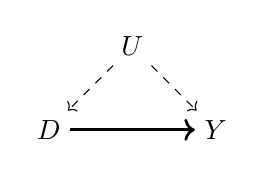
\begin{tikzpicture}[node distance=1.5cm]
	
		% nodes - for left-hand DAG %
		\node[text centered] (u) {$U$};
		\node[below right of  = u, text centered] (y) {$Y$};
		\node[below left of = u, text centered] (d) {$D$};
 
		% edges %
		\draw[->, line width=1] (d) -- (y);
		\draw[dashed, ->] (u) -- (y);
		\draw[dashed, ->] (u) -- (d);

		\end{tikzpicture}
		\end{center}
		\end{minipage}


	\end{center}

Then $D$ is endogenous due to backdoor path $D \leftarrow U \rightarrow Y$ and causal effect $D\rightarrow Y$ is not identified using the backdoor criterion.  

\end{frame}	


\begin{frame}[plain]

	\begin{center}
	\textbf{Instruments}
	\end{center}
	
	
	\begin{center}
	\begin{minipage}{.5\textwidth}
	
	\begin{center}
	
	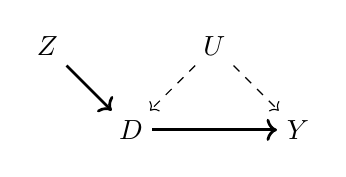
\begin{tikzpicture}[node distance=1.5cm]
	
		% nodes - for left-hand DAG %
		\node[text centered] (u) {$U$};
		\node[below right of  = u, text centered] (y) {$Y$};
		\node[below left of = u, text centered] (d) {$D$};
		\node[above left of = d, text centered] (z) {$Z$};
 
		% edges %
		\draw[->, line width=1] (d) -- (y);
		\draw[->, line width=1] (z) -- (d);
		\draw[dashed, ->] (u) -- (y);
		\draw[dashed, ->] (u) -- (d);

		\end{tikzpicture}
		\end{center}
		\end{minipage}


	\end{center}

	Notice how the path from $Z\rightarrow D\leftarrow U \rightarrow Y$ is blocked by a collider.  

\end{frame}	



\begin{frame}[plain]

	\begin{center}
	\textbf{Phillip Wright}
	\end{center}
	
	\begin{itemize}
	\item Philip Wright was a renaissance man - published in JASA, QJE, AER, you name it, while on a very intense teaching load. 
	\item Also published poetry, and even personally published Carl Sandburg's first book of poetry!
	\item Spent a long time at Tufts
	\item He was very concerned about the negative effects of tariffs and wrote a book about commodity markets
	\end{itemize}

\end{frame}

\begin{frame}[plain]
	\begin{center}
	\textbf{Elasticity of demand is unidentified}
	\end{center}
	
	\begin{itemize}
	\item James Stock notes that his publications had a theme regarding identification
	\item He knew, for instance, that he couldn't simple look at correlations between price and quantity if he wanted the elasticity of demand due to simultaneous shifts in supply and demand
	\item The pairs of quantity and price weren't demand, or supply - they were demand and supply equilibrium values and therefore didn't reflect the demand or the supply curve, both of which are counterfactuals
	\item Those points are nothing more than a bunch of numbers -- no more, no less -- that have no practical use, scientific or otherwise
	\end{itemize}
	
\end{frame}

\begin{frame}[plain]

 \begin{figure}[h]
\includegraphics[scale=0.75]{./lecture_includes/supply_demand.pdf}
\caption{Wright's graphical demonstration of the identification problem}
\label{fig:sd}
\end{figure}

\end{frame}

\begin{frame}[plain]
\begin{center}
\textbf{Sewell Wright}
\end{center}

\begin{itemize}
\item Sewell was his son, who did \emph{not} go into the family business
\item Rather, he decided to become a genius and invent genetics
\item Developed path diagrams (which Pearl revived 50 years later for causal inference) 
\item Father and son engage in letter correspondence as Philip tried to solve the ``identification problem''

\end{itemize}

\end{frame}

\begin{frame}[plain]


\centering
  \begin{overprint}%
\begin{figure}[h]
  \makebox[\textwidth][c]{\includegraphics[width=1.0\textwidth]{./lecture_includes/wright_letter.png}}%
\caption{Wright's letter to Sewell, his son}
\end{figure}
  \end{overprint}%

\end{frame}


\begin{frame}[plain]


\centering
  \begin{overprint}%
\begin{figure}[h]
  \makebox[\textwidth][c]{\includegraphics[width=1.0\textwidth]{./lecture_includes/path_diagrams_wrights.png}}%
\caption{Recognize these?}
\end{figure}
  \end{overprint}%

\end{frame}


\begin{frame}[plain]
\begin{center}
\textbf{QJE Rejects}
\end{center}

\begin{itemize}
\item QJE misses a chance to make history and rejects his paper proving an IV estimator
\item Sticks his proof in Appendix B of 1928 book, \underline{The Tariff on Animal and Vegetable Oils}
\item His work on IV is ignored, and is then rediscovered 15 years later (e.g., Olav Reiers\o l). 
\item James Stock and others have helped correct the record
\end{itemize}

\end{frame}


\begin{frame}[plain]
\begin{center}
\textbf{Sidebar: stylometric analysis}
\end{center}

\begin{itemize}
\item Long standing question was who \emph{wrote} Appendix B? Answer according to Stock and Trebbi (2003) using stylometric methods is that Philip \emph{wrote} it.
\item But who invented it?  It was collaborative, but Sewell acknowledged he didn't know how to handle endogeneity and simultaneity (that was Philip)
\end{itemize}

\end{frame}


\begin{frame}[plain]

	\begin{center}
	\textbf{Constant treatment effects}
	\end{center}

		\begin{itemize}
		\item Constant treatment effects (i.e., $\beta$ is constant across all individual units)
			\begin{itemize}
			\item Constant treatment effects is the traditional econometric pedagogy when first learning instrumental variables, and doesn't need the potential outcomes model or notation to get the point across
			\item Constant treatment effects is identical to assuming that ATE$=$ATT$=$ATU because constant treatment effects assumes $\beta_i=\beta_{-i}=\beta$ for all units
			\end{itemize}
		\end{itemize}

\end{frame}


\begin{frame}[plain]

\begin{center}
\textbf{Heterogenous treatment effects}
\end{center}

\begin{itemize}
		\item Heterogeneous treatment effects (i.e., $\beta_i$ varies across individual units)
			\begin{itemize}
			\item Heterogeneous treatment effects means that the $ATE\neq{ATT}\neq{ATU}$ because $\beta_i$ differs across the population
			\item This is equivalent to assuming the coefficient, $\beta_i$, is a random variable that varies across the population
			\item Heterogenous treatment effects is based on work by Angrist, Imbens and Rubin (1996) and Imbens and Angrist (1994) which introduced the  ``local average treatment effect'' (LATE) concept
			\end{itemize}
\end{itemize}

\end{frame}

\begin{frame}[plain]

\begin{center}
\textbf{Data requirements}
\end{center}

	\begin{itemize}
	\item Your data isn't going to come with a codebook saying ``instrumental variable''.  So how do you find it?
	\item Well, sometimes the researcher just \emph{knows}.  
	\item That is, the researcher knows of a variable ($Z$) that actually \emph{is} randomly assigned and that affects the endogenous variable but not the outcome (except via the endogenous variable)  
	\item Such a variable is called an ``instrument''.
	\end{itemize}
\end{frame}


\begin{frame}[plain]
\begin{center}
\textbf{Picking a good instrument}
\end{center}

	\begin{itemize}
	\item The best instruments you think of first, then you seek the data second (but often students go in the reverse order which is basically guaranteed to be a crappy instrument)
	\item If you want to use IV, then ask: 
		\begin{quote}
		What moves around the covariate of interest that might be plausibly random?
		\end{quote}
		\item Is there any element in the treatment that could be construed as random?  
		\item If you were to find that random piece, then you have found an instrument
	\item Once you have identified such a variable, begin to think about what data sets might have information on an outcome of interest, the treatment, and the instrument you have put your finger on.
	\end{itemize}
\end{frame}



\begin{frame}[plain]
\begin{center}
\textbf{Does family size reduce labor supply or is it selection?}
\end{center}

Angrist and Evans (1998), ``Children and their parents' labor supply'' \emph{American Economic Review}, 
		\begin{itemize}
		\item They want to know the effect of family size on labor supply, but need exogenous changes in family size
		\item So what if I told you if the first two children born were of the same gender, then you're less likely to work. What?!
		\end{itemize}

\end{frame}


\begin{frame}[plain]

\begin{center}
\textbf{Angrist and Evans cont.}
\end{center}

\begin{itemize}

		\item Many parents have a preference for having at least one child of each gender
			\begin{itemize}	
			\item Consider a couple whose first two kids were both boys; they will often have a third, hoping to have a girl
			\item Consider a couple whose first two kids were girls; they will often have a third, hoping for a boy
			\item Consider a couple with one boy and one girls; they will often not have a third kid
			\end{itemize}
		\item The gender of your kids is arguably randomly assigned (maybe not exactly, but close enough)
		\end{itemize}

\end{frame}



\begin{frame}[plain]
\begin{center}
\textbf{Good instruments must be a bit strange}
\end{center}

\begin{itemize}
		\item On its face, it's puzzling that the first two kids' gender predicts labor market participation
		\item Instrumental variables strategies formalize \emph{strangeness of the instrument}, which is the inference drawn by an intelligent layperson with no particular knowledge of the phenomena or background in statistics.
		\item You need more information, in other words, otherwise the layperson can't understand what same gender of your children has to do with working
\end{itemize}

\end{frame}

\begin{frame}[plain]
\begin{center}
\textbf{When a good IV strategy finally makes sense}
\end{center}

\begin{itemize}
		\item But then the researchers point out that women whose first two children are of the same gender are more likely to have additional children than women whose first two children are of different genders
		\item The layperson then asks himself, ``Hm. I wonder if the labor market differences are due \emph{solely} to the differences in the number of kids the woman has...''

\end{itemize}

\end{frame}

\begin{frame}[plain]
\begin{center}
\textbf{Sunday Candy is a good instrument}
\end{center}

\begin{itemize}
		\item Let's listen to a few lines from ``Ultralight Beam'' by Kanye West. Chance the Rapper sings on it and says

\begin{quote}
``I made Sunday Candy, I'm never going to hell \\


I met Kanye West, I'm never going to fail.'' \\


- Chance the Rapper
\end{quote}

	\item What does making a song have to do with hell?  What does meeting Kanye West have to do with success? Let's consider each in order
	\end{itemize}
\end{frame}

\begin{frame}[plain]
\begin{center}
\textbf{What are we missing?}
\end{center}

			\begin{quote}
			``I made Sunday Candy, \\
			I'm never going to hell'', 
			\end{quote}
		\begin{itemize}
		\item There must be more to this story, right?
		\item So what if it's something like this
		\end{itemize}
			\begin{quote}
			``I made Sunday Candy \\
			 this pastor invited me to church on Sunday, \\
			  I'm never going to hell''
			\end{quote}

\end{frame}




\begin{frame}[plain]

	\begin{center}
	\textbf{Sunday Candy DAG}
	\end{center}
	
	
	\begin{center}
	\begin{minipage}{.5\textwidth}
	
	\begin{center}
	
	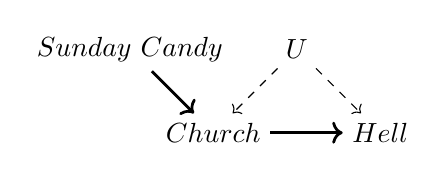
\begin{tikzpicture}[node distance=1.5cm]
	
		% nodes - for left-hand DAG %
		\node[text centered] (u) {$U$};
		\node[below right of  = u, text centered] (y) {$Hell$};
		\node[below left of = u, text centered] (d) {$Church$};
		\node[above left of = d, text centered] (z) {$Sunday\ Candy$};
 
		% edges %
		\draw[->, line width=1] (d) -- (y);
		\draw[->, line width=1] (z) -- (d);
		\draw[dashed, ->] (u) -- (y);
		\draw[dashed, ->] (u) -- (d);

		\end{tikzpicture}
		\end{center}
		\end{minipage}


	\end{center}


\end{frame}	


\begin{frame}[plain]
\begin{center}
\textbf{Kanye West is a bad instrument}
\end{center}

\begin{itemize}
\item Chance long idolized and was inspired by Kanye West -- both Chicago, both very creative hip hop artists
\item Kanye West is not a good instrument for Chance's inspiration, though, because Kanye West can singlehandedly make a person's career
\item Kanye is not strange enough
\end{itemize}

\end{frame}


\begin{frame}[plain]

	\begin{center}
	\textbf{Kanye West DAG}
	\end{center}
	
	
	\begin{center}
	\begin{minipage}{.5\textwidth}
	
	\begin{center}
	
	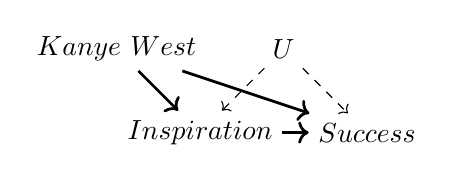
\begin{tikzpicture}[node distance=1.5cm]
	
		% nodes - for left-hand DAG %
		\node[text centered] (u) {$U$};
		\node[below right of  = u, text centered] (y) {$Success$};
		\node[below left of = u, text centered] (d) {$Inspiration$};
		\node[above left of = d, text centered] (z) {$Kanye\ West$};
 
		% edges %
		\draw[->, line width=1] (d) -- (y);
		\draw[->, line width=1] (z) -- (d);
		\draw[->, line width=1] (z) -- (y);
		\draw[dashed, ->] (u) -- (y);
		\draw[dashed, ->] (u) -- (d);

		\end{tikzpicture}
		\end{center}
		\end{minipage}


	\end{center}


\end{frame}	


\begin{frame}[plain]
\begin{center}
\textbf{Foreshadowing the questions you need to be asking}
\end{center}

\begin{enumerate}
	\item Is our instrument highly correlated with the treatment? With the outcome? Can you test that?
	\item Are there random elements within the treatment? Why do you think that?
	\item Is the instrument exogenous?  Why do you think that?
	\item Could the instrument affect outcomes directly? Why do you think that?
	\item Could the instrument be associated with anything that causes the outcome even if it doesn't directly? Why do you think that?
\end{enumerate}

\end{frame}




\begin{frame}[plain]
\begin{center}
\textbf{Our causal model: Returns to schooling again}
\end{center}\begin{eqnarray*}
Y = \alpha + \delta S + \gamma A + \nu
\end{eqnarray*}
where $Y$ is log earnings, $S$ is years of schooling, $A$ is unobserved ability, and $\nu$ is the error term

\begin{itemize}
	\item Suppose there exists a variable, $Z_i$, that is correlated with $S_i$ .
	\item We can estimate $\delta$ with this variable, $Z$:
\end{itemize}

\end{frame}


\begin{frame}[plain]

	\begin{center}
	\textbf{How can IV be used to obtain consistent estimates?}
	\end{center}
	
		\begin{eqnarray*}
		Cov(Y,Z) 	&=& Cov(\alpha + \delta{S} + \gamma{A} + \nu, Z) \\
				&=&	E[(\alpha + \delta{S} + \gamma{A} + \nu)  Z] - E[\alpha + \delta{S} + \gamma{A} + \nu]E[Z] \\
				&=& \{\alpha E(Z) - \alpha E(Z) \} + \delta \{ E(SZ) - E(S)E(Z)\} \\
				&& + \gamma \{E(AZ) - E(A)E(Z) \} + E(\nu Z) - E(\nu)E(Z) \\
		Cov(Y,Z)	&=& \delta Cov(S,Z) + \gamma Cov(A,Z) + Cov(\nu,Z)
		\end{eqnarray*}
		Divide both sides by $Cov(S,Z)$ and the first term becomes $\delta$, the LHS becomes the ratio of the reduced form to the first stage, plus two other scaled terms.
\end{frame}

\begin{frame}[plain]
\begin{center}
\textbf{Consistency}
\end{center}

	\begin{itemize}
	\item What conditions must hold for a valid IV design?
		\begin{itemize}
		\item  $Cov(S,Z)\neq{0}$ -- ``first stage'' exists.  $S$ and $Z$ are correlated 
		\item $Cov(A,Z)=Cov(\nu ,Z)=0$ -- ``exclusion restriction''.  This means $Z$ that orthogonal to the factors in $\nu$, such as unobserved ability, A, as well as the structural disturbance term, $\nu$
		\end{itemize}
	\item Assuming the first stage exists and that the exclusion restriction holds, then we can estimate $\delta$ with $\delta_{IV}$:
	\end{itemize}
	\begin{eqnarray*}
	\delta_{IV} &=& \frac{Cov(Y,Z)}{Cov(S,Z)} \\ 
	&=&\delta
	\end{eqnarray*}
\end{frame}





\begin{frame}[plain]

	\begin{center}
	\textbf{IV is Consistent if IV Assumptions are Satisfied}
	\end{center}
	
	\begin{itemize}
	\item The IV estimator is consistent if the IV assumptions are satisfied.  Substitute true model for $Y$:
		\begin{eqnarray*}
		\delta_{IV} &=& \frac{Cov([\alpha + \rho{S} + \gamma{A} + \nu],Z)}{Cov(S,Z)} \\
			&=& \delta \frac{Cov([S],Z)}{Cov(S,Z)} + \gamma \frac{Cov([A],Z)}{Cov(S,Z)} + \frac{Cov([\nu],Z)}{Cov(S,Z)} \\
			&=& \delta + \gamma \frac{Cov(\eta,Z)}{Cov(S,Z)}
		\end{eqnarray*}
	\end{itemize}
\end{frame}

\begin{frame}[plain]
\begin{center}
\textbf{Identifying assumptions and consistency}
\end{center}

\begin{itemize}
	\item Taking the probability limit which is an asymptotic operation to show consistency:\begin{eqnarray*}
	\text{plim }\widehat{\delta}_{IV}&=& \text{plim } \delta + \gamma \frac{Cov(\eta,Z)}{Cov(S,Z)} \\
	&=&\delta
	\end{eqnarray*}because $Cov([A],Z)=0$ and $Cov([\nu],Z)=0$ due to the exclusion restriction, and $Cov(S,Z)\neq{0}$ (due to the first stage)
\end{itemize}

\end{frame}

\begin{frame}[plain]
\begin{center}
\textbf{IV Assumptions}
\end{center}

\begin{itemize}
	\item But, if $Z$ is \emph{not} independent of $\eta$ (either correlated with $A$ or $\nu$), \emph{and} if the correlation between $S$ and $Z$ is ``weak'', then the second term blows up. 
	\item We will explore the problems created by weak instruments in just a moment. 
	\item First, let's look at a DAG summarizing all this information

\end{itemize}

\end{frame}


\begin{frame}[plain]

	\begin{center}
	\textbf{One of these DAGs is not like the other}
	\end{center}
	
	
	\begin{center}
	\begin{minipage}{.5\textwidth}
	
	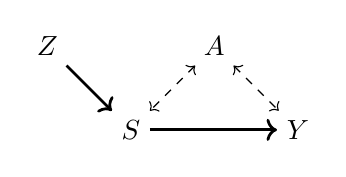
\begin{tikzpicture}[node distance=1.5cm]
	
		% nodes - for left-hand DAG %
		\node[text centered] (A) {$A$};
		\node[below right of  = A, text centered] (y) {$Y$};
		\node[below left of = A, text centered] (s) {$S$};
		\node[above left of = s, text centered] (z) {$Z$};
 
		% edges %
		\draw[->, line width=1] (s) -- (y);
		\draw[->, line width=1] (z) -- (s);
		\draw[dashed, <->] (A) -- (y);
		\draw[dashed, <->] (A) -- (s);

		\end{tikzpicture}
		\end{minipage}
\begin{center}
\emph{(a)}
\end{center}

  \vskip6pt plus.1fill
		
		\begin{minipage}{.5\textwidth}
		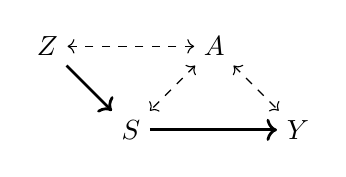
\begin{tikzpicture}[node distance=1.5cm]

		% nodes - for left-hand DAG %
		\node[text centered] (A) {$A$};
		\node[below right of  = A, text centered] (y) {$Y$};
		\node[below left of = A, text centered] (s) {$S$};
		\node[above left of = s, text centered] (z) {$Z$};
 
		% edges %
		\draw[->, line width=1] (s) -- (y);
		\draw[->, line width=1] (z) -- (s);
		\draw[dashed, <->] (A) -- (y);
		\draw[dashed, <->] (A) -- (s);
		\draw[dashed, <->] (A) -- (z);
		\end{tikzpicture}
		\end{minipage}
\begin{center}
\emph{(b)}
\end{center}

	\end{center}

Notice - the top DAG, \emph{a}, satisfies both exclusion and relevance (i.e., non-zero first stage), but the bottom DAG, \emph{b}, satisfies relevance but not exclusion.

\end{frame}

\subsection{Two stage least squares}

\begin{frame}

	\begin{center}
	\textbf{Two-stage least squares}
	\end{center}
	
	\begin{itemize}
	\item The two-stage least squares estimator was developed by Theil (1953) and Basman (1957) independently
	\item Note, while IV is a research design, 2SLS is a specific estimator. 
	\item Others include LIML, the Wald estimator, jacknive IV, two sample IV, and more
	\end{itemize}
\end{frame}

\begin{frame}[plain]
\begin{center}
\textbf{Two Sample IV}
\end{center}

	\begin{itemize}
	\item In a pinch, you can even get by with two different data sets
		\begin{enumerate}
		\item Dataset 1 needs information on the outcome and the instrument 
		\item Dataset 1 needs  information on the treatment and the instrument.
		\end{enumerate}
	\item This is known as ``Two sample IV'' because there are two \emph{samples} involved, rather than the traditional one sample.
	\item Once we define what IV is measuring carefully, you will see why this works.
	\end{itemize}
\end{frame}


\begin{frame}[plain]

	\begin{center}
	\textbf{Two-stage least squares concepts}
	\end{center}
	
	\begin{itemize}
	\item Causal model.  Sometimes called the structural model:$$Y_i=\alpha + \delta{S_i} + \eta_i$$
	\item First-stage regression. Gets the name because of two-stage least squares:$$S_i = \gamma + \rho{Z_i} + \zeta_i$$
	\item Second-stage regression. Notice the fitted values, $\widehat{S}$:$$Y_i=\beta + \delta{\widehat{S_i}}+\nu_i$$
	\end{itemize}
\end{frame}


\begin{frame}[plain]
\begin{center}
\textbf{Reduced form}
\end{center}

\begin{itemize}
\item Some people like a simpler approach because they don't want to defend IV's assumptions
\item Reduced form a regression of $Y$ onto the instrument:$$Y_i=\psi + \pi{Z_i} + \varepsilon_i$$
\item This would be like regressing hell onto Sunday Candy, as opposed to regressing hell onto church with Sunday Candy instrumenting for church
\end{itemize}

\end{frame}






\begin{frame}[plain]
\begin{center}
\textbf{Two-stage least squares}
\end{center}

Suppose you have a sample of data on $Y$, $X$, and $Z$. For each observation $i$ we assume the data are generated according to
		\begin{eqnarray*}
		Y_i &=& \alpha + \delta{S}_i + \eta_i \\
		S_i &=& \gamma + \rho{Z}_i + \zeta_i
		\end{eqnarray*}where $Cov(Z,\eta_i)=0$ and $\rho\neq{0}$.

\end{frame}


\begin{frame}[plain]
\begin{center}
\textbf{Two-stage least squares}
\end{center}

Plug in covariance and write out the following:
		\begin{eqnarray*}
		\widehat{\delta_{2sls}} &=& \frac{Cov(Z,Y)}{Cov(Z,S)} \\
		&=& \frac{ \frac{1}{n}\sum_{i=1}^n(Z_i - \overline{Z})(Y_i - \overline{Y})}{\frac{1}{n}\sum_{i=1}^n(Z_i - \overline{Z})(S_i - \overline{S})} \\
		&=& \frac{ \frac{1}{n} \sum_{i=1}^n(Z_i - \overline{Z})Y_i}{ \frac{1}{n} \sum_{i=1}^n (Z_i-\overline{Z})S_i}
		\end{eqnarray*}

\end{frame}

\begin{frame}[plain]
\begin{center}
\textbf{Two-stage least squares}
\end{center}

Substitute the causal model definition of $Y$ to get:
		\begin{eqnarray*}
		\widehat{\delta_{2sls} }&=& \frac{ \frac{1}{n} \sum_{i=1}^n (Z_i -\overline{Z})\{ \alpha + \delta{S}_i + \eta_i \}}{\frac{1}{n} \sum_{i=1}^n (Z_i - \overline{Z})S_i} \\
		&=& \delta + \frac{\frac{1}{n} (Z_i - \overline{Z})\eta_i}{\frac{1}{n}\sum_{i=1}^n(Z_i - \overline{Z})S_i} \\
		&=& \delta + \text{"small if \emph{n} is large"}
		\end{eqnarray*}Where did the first term go? Why did the second term become $\delta$?

\end{frame}	

\begin{frame}[plain]

	\begin{center}
	\textbf{Two-stage least squares}
	\end{center}

	\begin{itemize}

	\item Calculate the ratio of ``reduced form'' ($\pi$) to ``first stage'' coefficient ($\rho$):
		\begin{eqnarray*}
		\widehat{\delta}_{2sls} = \frac{ Cov(Z,Y)} {Cov(Z,S)} = \frac{ \frac{Cov(Z,Y)}{Var(Z)}}{ \frac{Cov(Z,S)}{Var(Z)}} = \frac{\widehat{\pi}}{\widehat{\rho}}
		\end{eqnarray*}
	\item Rewrite $\widehat{\rho}$ as\begin{eqnarray*}
	\widehat{\rho} &=&  \frac{Cov(Z,S)}{Var(Z)} \\
\widehat{\rho}Var(Z)	&=& Cov(Z,S) 
	\end{eqnarray*}
	\end{itemize}

\end{frame}


\begin{frame}[plain]
\begin{center}
\textbf{Two-stage least squares}
\end{center}

Then rewrite $\widehat{\delta}_{2sls}$
	\begin{eqnarray*}
	\widehat{\delta}_{2sls} &=& \frac{ Cov(Z,Y)}{ Cov(Z,S)} = \frac{\widehat{\rho}Cov(Z,Y)}{\widehat{\rho}Cov(Z,S)}= \frac{\widehat{\rho}Cov(Z,Y)}{\widehat{\rho}^2Var(Z)} \nonumber \\
	&=& \frac{Cov(\widehat{\rho}Z,Y)}{Var(\widehat{\rho}Z)} 
	\end{eqnarray*}


\end{frame}

\begin{frame}[plain]

	\begin{center}
	\textbf{Two-stage least squares}
	\end{center}
	
Recall $$S_i = \gamma + \rho{Z}_i + \zeta_i$$Then $$\widehat{S}=\widehat{\gamma} + \widehat{\rho}Z$$  
Then 
		\begin{eqnarray*}
		\widehat{\delta}_{2sls} &=& \frac{Cov(\widehat{\rho}Z,Y)}{Var(\widehat{\rho}Z)} =  \frac{Cov(\widehat{S},Y)}{Var(\widehat{S})}
		\end{eqnarray*}

\end{frame}


\begin{frame}[plain]

		\begin{proof}
		We will show that $\widehat{\delta}Cov(Y,Z) = Cov(\widehat{S},Y)$.  I will leave it to you to show that $Var(\widehat{\delta}Z) = Var(\widehat{S})$
		\begin{eqnarray*}
		Cov(\widehat{S},Y) &=& E[\widehat{S}Y] - E[\widehat{S}]E[Y] \\
		&=& E(Y[\widehat{\rho} + \widehat{\delta}Z]) - E(Y)E(\widehat{\rho} + \widehat{\delta}Z) \\
		&=& \widehat{\rho}E(Y) + \widehat{\delta}E(YZ) - \widehat{\rho}E(Y) - \widehat{\delta}E(Y)E(Z) \\
		&=&\widehat{\delta}[E(YZ) - E(Y)E(Z)] \\
		Cov(\widehat{S},Y) &=& \widehat{\delta}Cov(Y,Z)
		\end{eqnarray*}
		\qedhere
		\end{proof}

\end{frame}

\begin{frame}[plain]
	\begin{center}
	\textbf{Intuition of 2SLS}
	\end{center}
	
	\begin{itemize}
	\item Two stage least squares is nice because in addition to being an estimator, there's also great intuition contained in it which you can use as a device for thinking about IV more generally. 
	\item The intuition is that 2SLS estimator replaces $S$ with the fitted values of $S$ (i.e., $\widehat{S}$) from the first stage regression of $S$ onto $Z$ and all other covariates.  
	\item By using the fitted values of the endogenous regressor from the first stage regression, our regression now uses \emph{only} the exogenous variation in the regressor due to the instrumental variable itself
	\end{itemize}
\end{frame}

\begin{frame}[plain]
\begin{center}
\textbf{Intuition of IV in 2SLS}
\end{center}

\begin{itemize}
	\item \dots but think about it -- that variation was there before, but was just a subset of all the variation in the regressor
	\item Go back to what we said in the beginning - we need the endogenous variable to have pieces that are random, and IV finds them.
	\item Instrumental variables therefore reduces the variation in the data, but that variation which is left is 
\emph{exogenous}
	\item ``With a long enough [instrument], you can [estimate any causal effect]'' - Scott Cunningham paraphrasing Archimedes
\end{itemize}

\end{frame}
	




\begin{frame}[plain]

	\begin{center}
	\textbf{Estimation with software}
	\end{center}

	\begin{itemize}
	\item One manual way is just to estimate the reduced form and first stage coefficients and take the ratio of the respective coefficients on $Z$
	\item But while it is always a good idea to run these two regressions, don't compute your IV estimate this way 
	\end{itemize}
\end{frame}

\begin{frame}[plain]
\begin{center}
\textbf{Estimation with software}
\end{center}

\begin{itemize}
		\item It is often the case that a pattern of missing data will differ between $Y$ and $S$
		\item In such a case, the usual procedure of ``casewise deletion'' is to keep the subsample with non-missing data on $Y$, $S$, and $Z$.
		\item But the reduced form and first stage regressions would be estimated off of different sub-samples if you used the two step method before
		\item The standard errors from the second stage regression are also wrong
\end{itemize}

\end{frame}



\begin{frame}[plain]
\begin{center}
\textbf{Estimation with software}
\end{center}

\begin{itemize}

	\item Estimate this in Stata using -ivregress 2sls-.
	\item Estimate this in R -ivreg()- which is in the AER package

\end{itemize}

\end{frame}



\subsection{Weak instruments}

\begin{frame}
\begin{center}
\textbf{Weak instruments}
\end{center}

\begin{itemize}
\item A weak instrument is one that is not strongly correlated with the endogenous variable in the first stage
\item This can happen if the two variables are independent or the sample is small
\item If you have a weak instrument, then the bias of 2SLS is centered on the bias of OLS and the cure ends up being worse than the disease
\item We knew this was a problem, but it was brought into sharp focus with Angrist and Krueger (1991) and some papers that followed
\end{itemize}

\end{frame}

\begin{frame}[plain]

	\begin{center}
	\textbf{Angrist and Krueger (1991)}
	\end{center}
	
	\begin{itemize}
	\item In practice, it is often difficult to find convincing instruments -- usually because potential instruments don't satisfy the exclusion restriction
	\item But in an early paper in the causal inference movement, Angrist and Krueger (1991) wrote a very interesting and influential study instrumental variable 
	\item They were interested in schooling's effect on earnings and instrumented for it with \emph{which quarter of the year you were born}
	\item Remember Chance quote - what the heck would birth quarter have to do with earnings such that it was an excludable instrument?
	\end{itemize}
	
\end{frame}


\begin{frame}[plain]
\begin{center}
\textbf{Compulsory schooling}
\end{center}

\begin{itemize}

	\item In the US, you could drop out of school once you turned 16
	\item ``School districts typically require a student to have turned age six by January 1 of the year in which he or she enters school'' (Angrist and Krueger 1991, p. 980)
	\item Children have different ages when they start school, though, and this creates different lengths of schooling at the time they turn 16 (potential drop out age):
	\end{itemize}
	
\end{frame}

\begin{frame}[plain]
\begin{figure}[htb]
\centering
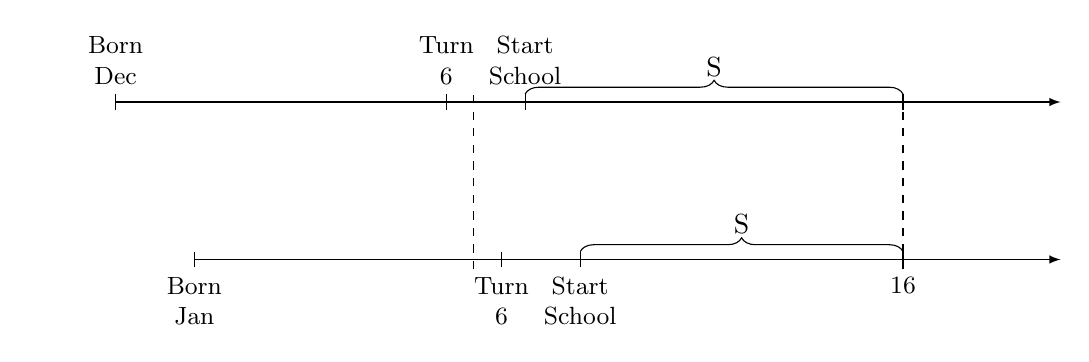
\begin{tikzpicture}
	\draw [-{latex}] (0,2) -- (12,2);
	\draw [-{latex}] (1,0) -- (12,0);
	
	\draw (0,1.9) -- (0,2.1) node [anchor=south, pos=1, text width=2cm, align=center, font=\small] {Born\\ Dec};
	\draw (4.2,1.9) -- (4.2,2.1) node [anchor=south, pos=1, text width=2cm, align=center, font=\small] {Turn\\ 6};
	\draw (5.2,1.9) -- (5.2,2.1) node [anchor=south, pos=1, text width=2cm, align=center, font=\small] {Start\\ School};
	\draw (10,1.9) -- (10,2.1);
	
	\draw (1,-0.1) -- (1,0.1) node [anchor=north, pos=0, text width=2cm, align=center, font=\small] {Born\\ Jan};
	\draw (4.9,-0.1) -- (4.9,0.1) node [anchor=north, pos=0, text width=2cm, align=center, font=\small] {Turn\\ 6};
	\draw (5.9,-0.1) -- (5.9,0.1) node [anchor=north, pos=0, text width=2cm, align=center, font=\small] {Start\\ School};
	\draw (10,-0.1) -- (10,0.1) node [anchor=north, pos=0, text width=2cm, align=center, font=\small] {16};
	
	\draw [dashed] (4.55,-0.125) -- (4.55,2.125);
	\draw [dashed] (10,-0.125) -- (10,2.125);
	
	\draw [decorate, decoration={brace, amplitude=5pt, raise=0pt}] (5.2,2.1) -- (10,2.1) node [pos=0.5,anchor=south, yshift=0.1cm] {S};
	\draw [decorate, decoration={brace, amplitude=5pt, raise=0pt}] (5.9,0.1) -- (10,0.1) node [pos=0.5,anchor=south, yshift=0.1cm] {S};
		
\end{tikzpicture}

\end{figure}
If you're born in the fourth quarter, you hit 16 with more schooling than those born in the first quarter
\end{frame}

\begin{frame}[plain]
\begin{center}
\textbf{Visuals}
\end{center}

\begin{itemize}
\item You need good data visualization for IV partly because of the scrutiny around the design
\item The two pieces you should be ready to build pictures for are the first stage and the reduced form
\item Angrist and Krueger (1991) provide simple, classic and compelling pictures of both
\end{itemize}

\end{frame}



\begin{frame}[plain]

	\begin{center}
	\textbf{First Stage}
	\end{center}
	
	 Men born earlier in the year have lower schooling. This indicates that there is a first stage. Notice all the 3s and 4s at the top. But then notice how it attenuates over time \dots
	
	\begin{figure}
	\includegraphics{./lecture_includes/qob_2.pdf}
	\end{figure}
	
\end{frame}


\begin{frame}[plain]

	\begin{center}
	\textbf{Reduced Form}
	\end{center}
	
	 Do differences in schooling due to different quarter of birth translate into different earnings?
	
	\begin{figure}
	\includegraphics{./lecture_includes/qob_3.pdf}
	\end{figure}
	
\end{frame}

\begin{frame}[plain]

	\begin{center}
	\textbf{Two Stage Least Squares model}
	\end{center}
	
	\begin{itemize}
	\item The causal model is $$Y_i = \delta S_i + \varepsilon$$
	\item The first stage regression is:$$S_i=X\pi_{10} + \pi_{11}Z_i + \eta_{1i}$$
	\item The reduced form regression is:$$Y_i=X\pi_{20} + \pi_{21}Z_i+\eta_{2i}$$
	\item The covariate adjusted IV estimator is the sample analog of the ratio, $\frac{\pi_{21}}{\pi_{11}}$
	\end{itemize}

\end{frame}

\begin{frame}[plain]

	\begin{center}
	\textbf{Two Stage Least Squares}
	\end{center}
	
	\begin{itemize}
	\item Angrist and Krueger instrument for schooling using three quarter of birth dummies:  a dummies for 2nd, 3rd and 4th qob
	\item Their estimated first-stage regression is:$$S_i=X\pi_{10} + Z_{1i}\pi_{11} + Z_{2i}\pi_{12} + Z_{3i}\pi_{13}+\eta_1$$
	\item The second stage is the same as before, but the fitted values are from the new first stage
	\end{itemize}

\end{frame}


\begin{frame}[plain]

	\begin{center}
	\textbf{First stage regression results}
	\end{center}

	 Quarter of birth is a strong predictor of total years of education
	
	\begin{figure}
	\includegraphics{./lecture_includes/qob_5.pdf}
	\end{figure}

\end{frame}

\begin{frame}[plain]

	\begin{center}
	\textbf{First stage regression results: Placebos}
	\end{center}
	
	\begin{figure}
	\includegraphics{./lecture_includes/qob_5b.pdf}
	\end{figure}
\end{frame}



\begin{frame}[plain]

	\begin{center}
	\textbf{IV Estimates Birth Cohorts 20-29, 1980 Census}
	\end{center}
	
	\begin{figure}
	\includegraphics{./lecture_includes/qob_7.pdf}
	\end{figure}
	
\end{frame}


	\begin{frame}[plain]
	\begin{center}
	\textbf{Sidebar: Wald estimator}
	\end{center}
	
	\begin{itemize}
	\item Recall that 2SLS uses the predicted values from a first stage regression -- but we showed that the 2SLS method was equivalent to $\frac{Cov(Y,Z)}{Cov(X,Z)}$
	\item The Wald estimator simply calculates the return to education as the ratio of the difference in earnings by quarter of birth to the difference in years of education by quarter of birth -- it's a version of the above
	\item Formally, $IV_{Wald} = \frac{E(Y|Z=1) - E(Y|Z=0)}{E(D|Z=1) - E(D|Z=0)}$
	\end{itemize}
\end{frame}



\begin{frame}[plain]
	\begin{center}
	\textbf{Mechanism}
	\end{center}
	
	\begin{itemize}
	\item In addition to log weekly wage, they examined the impact of compulsory schooling on log annual salary and weeks worked
	\item The main impact of compulsory schooling is on the log weekly wage -- not on weeks worked
	\end{itemize}
\end{frame}


\begin{frame}[plain]
\begin{center}
\textbf{More instruments}
\end{center}

	\begin{figure}
	\includegraphics[scale=.25]{./lecture_includes/weak_qob1.png}
	\end{figure}
	

\end{frame}


\begin{frame}[plain]

	\begin{center}
	\textbf{Problem enters with many quarter of birth interactions}
	\end{center}
	
	\begin{itemize}
	\item They want to increase the precision of their 2SLS estimates, so they load up their first stage with more instruments
	\item Specifications with 30 (quarter of birth $\times$ year) dummy variables and 150 (quarter of birth $\times$ state) instruments
		\begin{itemize}
		\item What's the intuition here?  The effect of quarter of birth may vary by birth year or by state
		\end{itemize}
	\item It reduced the standard errors, but that comes at a cost of potentially having a weak instruments problem
	\end{itemize}
	
\end{frame}




\begin{frame}[plain]
\begin{center}
\textbf{More instruments}
\end{center}

	\begin{figure}
	\includegraphics[scale=.25]{./lecture_includes/weak_qob2.png}
	\end{figure}
	

\end{frame}


\begin{frame}[plain]
\begin{center}
\textbf{More instruments}
\end{center}

	\begin{figure}
	\includegraphics[scale=.18]{./lecture_includes/weak_qob3.png}
	\end{figure}
	

\end{frame}


\begin{frame}[plain]

	\begin{center}
	\textbf{Weak Instruments}
	\end{center}
	
	\begin{itemize}
	\item For a long time, applied empiricists were not attentive to the small sample bias of IV
	\item But in the early 1990s, a number of papers highlighted that IV can be \emph{severely} biased -- in particular, when instruments have only a weak correlation with the endogenous variable of interest and when many instruments are used to instrument for one endogenous variable (i.e., there are many overidentifying restrictions).
	\item In the worst case, if the instruments are so weak that there is no first stage, then the 2SLS sampling distribution is centered on the probability limit of OLS
	\end{itemize}
\end{frame}

\begin{frame}[plain]

	\begin{center}
	\textbf{Causal model}
	\end{center}
	
	\begin{itemize}
	\item Let's consider a model with a single endogenous regressor and a simple constant treatment effect (i.e., ``just identified'')
	\item The causal model of interest is: $$Y=\beta X + \nu$$
	\end{itemize}
\end{frame}


\begin{frame}[plain]
\begin{center}
\textbf{Matrices and instruments}
\end{center}

\begin{itemize}
	\item We'll sadly need some matrix notation, but I'll try to make it painless.
	\item The matrix of instrumental variables is Z with the first stage equation:$$X = {Z'}\pi + \eta$$
	\item And let $P_z$ be the project matrix producing residuals from population regression of $X$ on $Z$ $$P_z=Z(Z'Z)^{-1}Z'$$
\end{itemize}

\end{frame}

\begin{frame}[plain]
\begin{center}
	\textbf{Weak instruments and bias towards OLS}
\end{center}

\begin{itemize}
	\item If $\nu_i$ and $\eta_i$ are correlated, estimating the first equation by OLS would lead to biased results, wherein the OLS bias is:$$E[\beta_{OLS} - \beta] = \frac{ Cov(\nu, X)}{Var(X)}$$
	\item If $\nu_i$ and $\eta_i$ are correlated the OLS bias is therefore: $\frac{\sigma_{\nu \eta}}{\sigma^2_\eta}$
\end{itemize}

\end{frame}


\begin{frame}[plain]
\begin{center}
\textbf{Deriving the bias of 2SLS}
\end{center}

\begin{eqnarray*}
\widehat{\beta}_{2sls} &=& (X'P_zX)^{-1}X'P_ZY \\
&=& \beta + (X'P_zX)^{-1}X'PZ_z \nu
\end{eqnarray*}substitution of $Y=\beta X + \nu$

\end{frame}


\begin{frame}[plain]
\begin{center}
\textbf{2SLS bias}
\end{center}

\begin{eqnarray*}
\widehat{\beta}_{2sls} - \beta &=& (X'P_zX)^{-1}X'P_z\nu \\
&=&aX'P_z \nu \\
&=&a[\pi ' Z' + \eta ']P_z \nu \\
&=&a \pi' Z' \nu + a \eta ' P_Z \nu \\
&=& (X'P_Z X)^{-1} \pi ' Z ' \nu + (X'P_zX)^{-1} \eta ' P_z \nu
\end{eqnarray*}

The bias of 2SLS comes from the non-zero expectation of terms on the right-hand-side even though $Z$ and $\nu$ are not correlated. 

\end{frame}


\begin{frame}[plain]
\begin{center}
\textbf{Taking expectations}
\end{center}

\begin{itemize}
\item Angrist and Pischke (ch. 4) note that taking expectations of that prior expression is hard because the expectation operator won't pass through $(X'P_zX)^{-1}$. 
\item However, the expectation of the ratios in the second term can be closely approximated
\end{itemize}

\begin{eqnarray*}
\widehat{\beta}_{2sls} - \beta  &=& (X'P_Z X)^{-1} \pi ' Z ' \nu + (X'P_zX)^{-1} \eta ' P_z \nu \\
E [ \widehat{\beta}_{2sls} - \beta ] &\approx & \bigg (E[X'P_Z X] \bigg ) ^{-1} E [\pi ' Z ' \nu ] + \bigg ( E [ X'P_zX] \bigg ) ^{-1}  E [ \eta ' P_z \nu ]
\end{eqnarray*}

\end{frame}

\begin{frame}[plain]
\begin{center}
\textbf{Approximate bias of 2SLS}
\end{center}

We know $E[\pi ' Z ' \nu ] =0$ and $E[ \pi ' Z ' \eta ] = 0$. So letting $E [ \eta ' P_z \nu ] = b$ bc this is hard for me otherwise

\begin{eqnarray*}
E [ \widehat{\beta}_{2sls} - \beta ] &\approx & E[X'P_z X)^{-1} b \\
& \approx & E 9 X' Z(Z'Z)^{-1} Z' X)^{-1} b \\
& \approx & E [ ( \pi Z + \eta ) ' P_z (\pi Z + \eta)]^{-1} b \\
& \approx & \bigg(  E (\pi ' Z'Z \pi) + E(\eta ' P_z \eta)^{-1} \bigg ) b \\
& \approx & \bigg ( E (\pi ' Z'Z \pi) + E(\eta ' P_z \eta)^{-1} \bigg ) E [ \eta ' P_z \nu ]  \\
\end{eqnarray*}

That last term is what creates the bias so long as $\eta$ and $\nu$ are correlated -- which it's because they are that you picked up 2SLS to begin with

\end{frame}


\begin{frame}[plain]
\begin{center}
\textbf{First stage F}
\end{center}

With some algebra and manipulation, Angrist and Pische show that the bias of 2SLS is equal to

\begin{eqnarray*}
E [ \widehat{\beta}_{2sls} - \beta ] &\approx &  \frac{\sigma_{\nu \eta}}{\sigma^2_\eta} \bigg [ \frac{E(\pi ' Z ' Z \pi)/Q}{\sigma^2_{\eta}} + 1 \bigg ]^{-1}
\end{eqnarray*}where the interior term is the population F-statistic for the joint significance of all regressions in the first stage

\end{frame}

\begin{frame}[plain]

	\begin{center}
	\textbf{Weak instruments and bias towards OLS}
	\end{center}
	
	\begin{itemize}
	\item Substituting $F$ for that big term, we can derive the approximate bias of 2SLS as:$$E[\widehat{\beta}_{2SLS} - \beta] \approx \frac{\sigma_{\nu \eta}}{\sigma^2_\eta} \frac{1}{F+1}$$
	\item Consider the intuition all that work bought us now: if the first stage is weak (i.e, $F\rightarrow{0}$), then the bias of 2SLS approaches $\frac{\sigma_{\nu \eta}}{\sigma^2_\eta}$
	\end{itemize}
\end{frame}

\begin{frame}[plain]

\begin{center}
\textbf{Weak instruments and bias towards OLS}
\end{center}

\begin{itemize}
	\item This is the same as the OLS bias as for $\pi=0$ in the second equation on the earlier slide (i.e., there is no first stage relationship) $\sigma^2_x = \sigma^2_\eta$ and therefore the OLS bias $\frac{\sigma_{\nu \eta}}{\sigma^2_\eta}$ becomes $\frac{\sigma_{\nu \eta}}{\sigma^2_\eta}$.
	\item But if the first stage is very strong ($F\rightarrow{\infty}$) then the 2SLS bias is approaching 0.
	\item Cool thing is -- you can test this with an F test on the joint significance of $Z$ in the first stage
	\item It's absolutely critical therefore that you choose instruments that are strongly correlated with the endogenous regressor, otherwise the cure is worse than the disease
\end{itemize}

\end{frame}

\begin{frame}[plain]

	\begin{center}
	\textbf{Weak Instruments - Adding More Instruments}
	\end{center}
	
	\begin{itemize}
	\item Adding more weak instruments will increase the bias of 2SLS
		\begin{itemize}
		\item By adding further instruments without predictive power, the first stage $F$-statistic goes toward zero and the bias increases
		\item We will see this more closely when we cover judge fixed effects
		\end{itemize}
	\item If the model is ``just identified'' -- mean the same number of instrumental variables as there are endogenous covariates -- weak instrument bias is less of a problem
	\end{itemize}
\end{frame}

\begin{frame}[plain]
\begin{center}
\textbf{Weak instrument problem}
\end{center}

\begin{itemize}
	\item After Angrist and Krueger study, there were new papers highlighting issues related to weak instruments and finite sample bias
	\item Key papers are Nelson and Startz (1990), Buse (1992), Bekker (1994) and especially Bound, Jaeger and Baker (1995)
	\item Bound, Jaeger and Baker (1995) highlighted this problem for the Angrist and Krueger study.  
\end{itemize}

\end{frame}

\begin{frame}[plain]
\begin{center}
\textbf{Bound, Jaeger and Baker (1995)}
\end{center}

Remember, AK present findings from expanding their instruments to include many interactions
		\begin{enumerate}
		\item Quarter of birth dummies $\rightarrow$ 3 instruments
		\item Quarter of birth dummies $+$ (quarter of birth) $\times$ (year of birth) $+$ (quarter of birth) $\times$ (state of birth) $\rightarrow$ 180 instruments
		\end{enumerate}
So if any of these are weak, then the approximate bias of 2SLS gets worse

\end{frame}


\begin{frame}[plain]

	\begin{center}
	\textbf{Adding instruments in Angrist and Krueger}
	\end{center}
	
	\begin{figure}
	\includegraphics{./lecture_includes/ak_iv1.pdf}
	\end{figure}
	
Adding more weak instruments reduced the first stage $F$-statistic and increases the bias of 2SLS. Notice its also moved closer to OLS. 
	
\end{frame}

\begin{frame}[plain]

	\begin{center}
	\textbf{Adding instruments in Angrist and Krueger}
	\end{center}
	
	\begin{figure}
	\includegraphics{./lecture_includes/ak_iv2.pdf}
	\end{figure}
	
More instruments increase precision, but drive down $F$, therefore we know the problem has gotten worse
	
\end{frame}


\begin{frame}[plain]

	\begin{center}
	\textbf{Guidance on working around weak instruments}
	\end{center}
	
		\begin{itemize}
		\item Use a just identified model with your strongest IV
		\item Use a limited information maximum likelihood estimator (LIML) as it is approximately median unbiased for over identified constant effects models and provides the same asymptotic distribution as 2SLS (under constant effects) with a finite-sample bias reduction. 
		\item Find stronger instruments -- easier said than done
		\end{itemize}
\end{frame}


\subsection{Practical IV Tips}


\begin{frame}
\begin{center}
\textbf{Look at the reduced form}
\end{center}

\begin{enumerate}
	\item Look at the reduced form
		\begin{itemize}
		\item The reduced form is estimated with OLS and is therefore unbiased
		\item If you can't see the causal relationship of interest in the reduced form, it is probably not there
		\end{itemize}
\end{enumerate}

\end{frame}

\begin{frame}[plain]
	\begin{center}
	\textbf{Report the first stage}
	\end{center}
	
	\begin{enumerate}\addtocounter{enumi}{1}
	\item Report the first stage (preferably in the same table as your main results)
		\begin{itemize}
		\item Does it make sense?
		\item Do the coefficients have the right magnitude and sign?
		\item Please make beautiful IV tables -- you'll be celebrated across the land if you do
		\end{itemize}
	\end{enumerate}
\end{frame}


\begin{frame}[plain]
\begin{center}
\textbf{Report $F$ statistic and OLS}
\end{center}

	\begin{enumerate}\addtocounter{enumi}{2}
	\item Report the $F$-statistic on the excluded instrument(s).
		\begin{itemize}
		\item Stock, Wright and Yogo (2002) suggest that $F$-statistics $>10$ indicate that you do not have a weak instrument problem -- this is not a proof, but more like a rule of thumb
		\item If you have more than one endogenous regressor for which you want to instrument, reporting the first stage $F$-statistic is not enough (because 1 instrument could affect both endogenous variables and the other could have no effect -- the model would be under identified). In that case, you want to report the Cragg-Donald EV statistic.
		\end{itemize}
	\item Report OLS -- you said it was biased, but we want to still see it
	\end{enumerate}

\end{frame}



\begin{frame}[plain]

\begin{table}[htbp]\centering
\scriptsize
\caption{OLS and 2SLS regressions of Log Earnings on Schooling}
\label{2sls_1}
\begin{center}
\begin{threeparttable}
\begin{tabular}{l*{2}{c}}
\toprule
\multicolumn{1}{l}{\textbf{Dependent variable}}&
\multicolumn{2}{c}{\textbf{Log wage}}\\
\multicolumn{1}{c}{}&
\multicolumn{1}{c}{OLS}&
\multicolumn{1}{c}{2SLS}\\
\midrule
educ                &       0.071***&       0.124** \\
                    &     (0.003)   &     (0.050)   \\
exper               &       0.034***&       0.056***\\
                    &     (0.002)   &     (0.020)   \\
black               &      -0.166***&      -0.116** \\
                    &     (0.018)   &     (0.051)   \\
south               &      -0.132***&      -0.113***\\
                    &     (0.015)   &     (0.023)   \\
married             &      -0.036***&      -0.032***\\
                    &     (0.003)   &     (0.005)   \\
smsa                &       0.176***&       0.148***\\
                    &     (0.015)   &     (0.031)   \\
\\
\midrule
\multicolumn{1}{c}{First Stage Instrument}\\
College in the county&               &       0.327***\\
Robust standard error &               &       0.082   \\
F statistic for IV in first stage&               &      15.767   \\
N                   &       3,003   &       3,003   \\
Mean Dependent Variable&       6.262   &       6.262   \\
Std. Dev. Dependent Variable&       0.444   &       0.444   \\
\bottomrule
\end{tabular}
\begin{tablenotes}
\tiny
\item Standard errors in parenthesis. * p$<$0.10, ** p$<$0.05, *** p$<$0.01
\end{tablenotes}
\end{threeparttable}
\end{center}
\end{table}

\end{frame}



\begin{frame}[plain]
	\begin{center}
	\textbf{Practical Tips for IV Papers}
	\end{center}
	
	\begin{enumerate}\addtocounter{enumi}{4}
	\item If you have many IVs, pick your best instrument and report the just identified model (weak instrument problem is much less problematic)
	\item Check over identified 2SLS models with LIML
	\end{enumerate}
\end{frame}


\begin{frame}[plain]
\begin{center}
\textbf{Make beautiful pictures of first stage and reduced form}
\end{center}

\begin{enumerate}\addtocounter{enumi}{6}
\item This cannot be overstated: you must present your main results in beautiful pictures
	\begin{itemize}
	\item Show pictures of the first stage. Convince the reader something is there.  The eyeball is underrated
	\item You can't show a second stage with raw data, so instead show pictures of the reduced form. 
	\end{itemize}
\end{enumerate}

\end{frame}




\begin{frame}[plain]

	\begin{center}
	\textbf{Visualizing the instrument: supply shocks on meth prices}
	\end{center}
	
	\begin{figure}
	\includegraphics[scale=0.15]{./lecture_includes/keith_1.png}
	\end{figure}
	
\end{frame}


\begin{frame}[plain]

	\begin{center}
	\textbf{Visualizing the first stage}
	\end{center}
	
	\begin{figure}
	\includegraphics[scale=0.15]{./lecture_includes/keith_3.png}
	\end{figure}
	
\end{frame}

\begin{frame}[plain]

	\begin{center}
	\textbf{Visualizing the reduced form}
	\end{center}
	
	\begin{figure}
	\includegraphics[scale=0.15]{./lecture_includes/keith_2.png}
	\end{figure}
	
\end{frame}


\subsection{Heterogeneity and the LATE}


\begin{frame}

	\begin{center}
	\textbf{Heterogenous Treatment Effects}
	\end{center}

	\begin{itemize}
	\item Up to this point, we only considered models where the causal effect was the same for all individuals 
		\begin{itemize}
		\item Constant treatment effects where $Y_{i}^1 - Y_i^0=\delta$ for all $i$ units)
		\end{itemize}
	\item Let's now try to understand what instrumental variables estimation is measuring if treatment effects are \emph{heterogenous} 
		\begin{itemize}
		\item $Y_i^1 - Y_i^0=\delta_i$ which varies across the population
		\end{itemize}
	\end{itemize}

\end{frame}

\begin{frame}[plain]
\begin{center}
\textbf{Why do we care about heterogeneity?}
\end{center}

\begin{itemize}
\item Heterogeneity, it turns out, makes life interesting and challenging
\item There are two issues here:
		\begin{enumerate}
		\item \underline{We care about internal validity}:  Does the design successfully uncover causal effects for the population that we are studying?
		\item \underline{We care about external validity}: Does the study's results inform us about different populations?
		\end{enumerate}
\item What parameter did we even estimate using IV when there were heterogenous treatment effects?
\end{itemize}

\end{frame}


\begin{frame}[plain]

	\begin{center}
	\textbf{Potential outcome notation}
	\end{center}
	
``Potential treatment status'' ($D^j$) versus ``observed'' treatment status ($D$)
		\begin{itemize}
		\item $D^1_{i} = i$'s treatment status when $Z_i=1$
		\item $D^0_{i} = i$'s treatment status when $Z_i=0$
		\end{itemize}
We'll represent outcomes as a function of both treatment status and instrument status. In other words, $Y_i(D_i=0,Z_i=1)$ is represented as $Y_i(0,1)$

\end{frame}


\begin{frame}[plain]
\begin{center}
\textbf{Switching equation}
\end{center}

Move from potential treatment status to observed treatment status
			\begin{eqnarray*}
			D_i&=&D^0_{i} + (D^1_{i} - D^0_{i})Z_i \\
			&=&\pi_{0i} + \pi_{1i}Z_i + \zeta_i
			\end{eqnarray*}
			\begin{eqnarray*}
			\pi_{0i} &=& E[D^0_{i}] \\
			\pi_{1i} &=& (D^1_{i} - D^0_{i}) \text{ is the heterogenous causal effect of the IV} \\
			&&\text{on }D_i. \\
			E[\pi_{1i}] &=& \text{The average causal effect of }Z_i\text{ on }D_i
			\end{eqnarray*}

\end{frame}


%\begin{frame}[plain]
%\begin{center}
%\textbf{Before we begin}
%\end{center}

%	\begin{block}{Intention-to-treat effects}
%	Causal effect of $Z$ on $D$ is $D^1_i - D^0_i$ \\
%	Causal effect of $Z$ on $Y$ is $Y_i(D^1_i,1) - Y_i(D^0_i,0)$
%	\end{block}


%\begin{itemize}
%\item Not uncommon for people to report the ITT, which is just the reduced form regression of Y on Z directly. 
%\item The reason you might do this is if you know the randomized treatment, but you're not sure of treatment participation.
%\item Maybe you're randomly assigned to classrooms as we saw with Krueger's STAR study, but you're not sure if people remained in those classes, or whatever. 
%\item Since you know the instrument is random, and that it's probably related to treatment takeup, then you might just report ITT
%\end{itemize}

%\end{frame}

\begin{frame}[plain]

	\begin{center}
	\textbf{Identifying assumptions under heterogenous treatment effects}
	\end{center}
		
	\begin{enumerate}
	\item Stable Unit Treatment Value Assumption (SUTVA)
	\item Random Assignment
	\item Exclusion Restriction
	\item Nonzero First Stage
	\item Monotonicity
	\end{enumerate}
\end{frame}


\begin{frame}[plain]

	\begin{center}
	\textbf{Stable Unit Treatment Value Assumption (SUTVA)}
	\end{center}
	
	\begin{block}{Stable Unit Treatment Value Assumption (SUTVA)}
	If $Z_i=Z_i'$, then $D_i(\textbf{Z})=D_i(\textbf{Z}')$ \\
	If $Z_i=Z_i'$ and $D_i=D_i'$, then $Y_i(\textbf{D,Z})=Y_i(\textbf{D',Z'})$
	\end{block}
	
 	\vskip3pt plus.1fill

\begin{itemize}
\item Potential outcomes for each person $i$ are unrelated to the treatment status of other individuals.
\item Example:   Your instrument is the death of a CEO for hirings. But if a CEO dies, then perhaps other companies lose a CEO as they are hired in the vacant spots.
\item In which case, the instrument is related to treatment status of other individuals.
\end{itemize}	
		
\end{frame}


\begin{frame}[plain]

	\begin{center}
	\textbf{Independence assumption}
	\end{center}
	
	\begin{block}{Independence assumption (e.g., ``as good as random assignment'')}
	$\{Y_i(D^1_i,1),Y_i(D^0_i,0),D^1_{i},D^{0}_i\} \independent{Z}_i$
	\end{block}

\begin{itemize}	
\item The IV is independent of the vector of potential outcomes and potential treatment assignments (i.e. ``as good as randomly assigned'') 
\item First two children of the same gender are assigned to families randomly. That is, they are assigned to those with higher likelihood of working just as often as it is assigned to those less likely to work.
\item It's all about the \emph{randomness} of the instrument, in other words, not the instrument's effect.
\end{itemize}

\end{frame}


\begin{frame}[plain]
\begin{center}
\textbf{Independence}
\end{center}

		 Independence means that the first stage measures the causal effect of $Z_i$ on $D_i$:
			\begin{eqnarray*}
			E[D_i|Z_i=1] - E[D_i|Z_i=0] &=& E[D^1_{i} | Z_i = 1] - E[D^0_{i}|Z_i = 0] \\
			&=& E[D^1_{i} - D^0_{i}]
			\end{eqnarray*}

\end{frame}

\begin{frame}[plain]
\begin{center}
\textbf{Independence}
\end{center}

	The  independence assumption is sufficient for a causal interpretation of the reduced form:
			\begin{eqnarray*}
			E[Y_i | Z_i=1] - E[Y_i | Z_i=0] &=& E[Y_i(D^1_{i},1)|Z_i = 1] \\
			&& - E[Y_i(D^0_{i},0) | Z_i = 0] \\
			&=&E[Y_i(D^1_{i},1)] - E[Y_i(D^0_{i},0)]
			\end{eqnarray*}
\end{frame}

\begin{frame}[plain]
\frametitle{Exclusion Restriction}

	\begin{block}{Exclusion Restriction}
	$\textbf{Y(D,Z)}=\textbf{Y(D,Z')}$ for all $\textbf{Z}$, $\textbf{Z'}$, and for all $\textbf{D}$
	\end{block}
	
\begin{itemize}
\item Any effect of $Z$ on $Y$ must be via the effect of $Z$ on $D$. In other words, $Y_i(D_i,Z_i)$ is a function of $D$ only.  Or formally:$$Y_i(D_i,0)=Y_i(D_i,1) \text{ for }D=0,1$$
\item Sometimes called the ``only through'' assumption because you're assuming the effect of $Z$ on $Y$ is ``only through'' its effect on $D$.
\item Recall the DAG and the \emph{missing arrows} from $Z$ to $u$ and from $Z$ to $Y$.
\end{itemize}
	
\end{frame}





\begin{frame}[plain]

	\begin{center}
	\textbf{Exclusion restriction}
	\end{center}
	
	\begin{itemize}
	\item Use the exclusion restriction to define potential outcomes indexed solely against treatment status: 
		\begin{eqnarray*}
		 Y^1_{i} &=& Y_i(1,1) = Y_i(1,0) \\
		 Y^0_{i} &=& Y_i(0,1) = Y_i(0,0)
		\end{eqnarray*}
	\item Rewrite the switching equation:
		\begin{eqnarray*}
		Y_i &=& Y_i(0,Z_i) + [Y_i(1,Z_i) - Y_i(0,Z_i)]D_i \\
		Y_i &=& Y^0_{i} + [Y^1_{i} - Y^0_{i}]D_i
		\end{eqnarray*}
	\item Random coefficients notation for this is:
		\begin{align*}
		&Y_i = \alpha_0 + \delta_iD_i& \\
		&\text{with }\alpha_0	= E[Y^0_{i}]\text{ and }\delta_i = Y^1_{i} - Y^0_{i}
		\end{align*}
	\end{itemize}

\end{frame}

\begin{frame}[plain]
\begin{center}
\textbf{Spotting violations of exclusion is a sport}
\end{center}

Watch the gears turn:
\begin{itemize}
\item We are interested in causal effect of military service on earnings, and so use draft number are instrument for military service. 
\item Draft number is generated by a random number generator. Therefore independence is met as draft number is independent of potential outcomes and potential treatment status. 
\item But, people with higher draft numbers evade draft by investing in schooling. Earnings change for reasons other than military service. Exclusion is violated
\item In other words, random lottery numbers (independence) do not imply that the exclusion restriction is satisfied
\end{itemize}

\end{frame}


\begin{frame}[plain]

	\begin{center}
	\textbf{Strong first stage}
	\end{center}
	
	\begin{block}{Nonzero Average Causal Effect of $Z$ on $D$}
	$E[D^1_{i} - D^0_{i}]\neq{0}$
	\end{block}
				
\begin{itemize}
\item $D^1$ means instrument is turned on, and $D^0$ means it is turned off. We need treatment to change when instrument changes.
\item $Z$ has to have some statistically significant effect on the average probability of treatment
\item First two children of the same gender makes you more likely to have a third.
\item Finally -- a testable assumption. We have data on $Z$ and $D$
\end{itemize}

\end{frame}			


\begin{frame}[plain]

	\begin{center}
	\textbf{Monotonicity}
	\end{center}
	
	\begin{block}{Monotonicity}
	Either $\pi_{1i}\geq{0}$ for all $i$ or $\pi_{1i}\leq{0}$ for all $i=1, \dots, N$
	\end{block}

\begin{itemize}

\item Recall that $\pi_{1i}$ is the reduced form causal effect of the instrumental variable on an individual $i$'s treatment status.  
\item Monotonicity requires that the instrumental variable (weakly) operate in the same direction on all individual units.  
\item In other words, while the instrument may have no effect on some people, all those who are affected are affected \emph{in the same direction} (i.e., positively or negatively, but not both).

\end{itemize}

\end{frame}

\begin{frame}[plain]
\begin{center}
\textbf{Monotonicity cont.}
\end{center}

\begin{itemize}
	
\item We instrument for schooling with birth quarter. Under monotonicity scenarios 1-2: 
	\begin{enumerate}
	\item they get more schooling or the same schooling if born in the fourth quarter
	\item they get less schooling or the same schooling if born in the fourth quarter
	\end{enumerate}
\item Monotonicity says either of these can be true, but they cannot both be true in your data -- yet it's not hard to imagine violations where two people respond differently  
\item Without monotonicity, IV estimators are not guaranteed to estimate a weighted average of the underlying causal effects of the affected group, $Y^1_{i} - Y^0_{i}$.
\end{itemize}

\end{frame}

\begin{frame}[plain]
\begin{center}
\textbf{Force yourself to think of monotonicity violations}
\end{center}

\begin{itemize}
			
\item  In the quarter of birth example for schooling, this assumption may not be satisfied (see Barua and Lang 2009).  
\item Being born in the $4^{th}$ quarter (which typically increases schooling) may have reduced schooling for some because their school enrollment was held back by their parents

\end{itemize}

\end{frame}



\begin{frame}[plain]
	\begin{center}
	\textbf{Local average treatment effect}
	\end{center}

	If all 1-5 assumptions are satisfied, then IV estimates the \textbf{local average treatment effect (LATE)} of $D$ on $Y$: $$\delta_{IV,LATE} =\frac{\text{Effect of Z on Y}}{\text{Effect of Z on D}}$$

\end{frame}	

\begin{frame}[plain]
\begin{center}
\textbf{Estimand}
\end{center}

	\vskip3pt plus.1fill
				
	Instrumental variables (IV) estimand: 
	\begin{align*}
	\delta_{IV,LATE} & = \frac{E[Y_i(D^1_i, 1) - Y_i(D^0_i, 0)]}{E[D^1_i - D^0_i]}& \\
	& = E[(Y^1_i - Y^0_i) | D^1_i - D^0_i = 1]
	\end{align*}

\end{frame}		

\begin{frame}[plain]

	\begin{center}
	\textbf{Local Average Treatment Effect}
	\end{center}
	
	\begin{itemize}
	\item The LATE parameters is the average causal effect of $D$ on $Y$ for those whose treatment status was changed by the instrument, $Z$
	\item For example, IV estimates the average effect of military service on earnings for the subpopulation who enrolled in military service because of the draft but would not have served otherwise. 
	\item LATE does not tell us what the causal effect of military service was for patriots (volunteers) or those who were exempted from military service for medical reasons 
	\end{itemize}
	
\end{frame}

\begin{frame}[plain]
\begin{center}
\textbf{LATE cont.}
\end{center}

\begin{itemize}

	\item We have reviewed the properties of IV with heterogenous treatment effects using a very simple dummy endogenous variable, dummy IV, and no additional controls example.  
	\item The intuition of LATE generalizes to most cases where we have continuous endogenous variables and instruments, and additional control variables.

\end{itemize}

\end{frame}

\begin{frame}[plain]	

	\begin{center}
	\textbf{LATE and subpopulations}
	\end{center}
	
The instrument partitions any population into 4 distinct groups:
		\begin{enumerate}
		\item \underline{Compliers}: The subpopulation with $D_i^1=1$ and $D_i^0=0$. Their treatment status is affected by the instrument in the ``correct direction''.
		\item \underline{Always takers}: The subpopulation with $D^1_{i}=D^0_{i}=1$. They always take the treatment independently of $Z$.
		\item \underline{Never takers}: The subpopulation with $D^1_{i}=D^0_{i}=0$. They never take the treatment independently of $Z$.
		\item \underline{Defiers}: The subpopulation with $D^1_{i}=0$ and $D^0_{i}=1$. Their treatment status is affected by the instrument in the ``wrong direction''.
		\end{enumerate}
\end{frame}

\begin{frame}[plain]	

	\begin{center}
	\textbf{Subpopulations of soldieres}
	\end{center}
	
Examples of subpopulations:
		\begin{enumerate}
		\item \underline{Compliers}: I only enrolled in the military because I was drafted otherwise I wouldn't have served
		\item \underline{Always takers}: My family have always served, so I serve regardless of whether I am drafted
		\item \underline{Never takers}: I'm a contentious objector so under no circumstances will I serve, even if drafted
		\item \underline{Defiers}: When I was drafted, I dodged. But had I not been drafted, I would have served. I can't make up my mind.
		\end{enumerate}
\end{frame}


\begin{frame}[plain]
	\begin{columns}[t]
	\scriptsize
	\column{.4\textwidth}
	\begin{block}{Never-Takers}
		$D^1_i - D^0_i = 0$ \\
		$Y_i(0,1) - Y_i(0,0) = 0$ \\
		By \textcolor{red}{Exclusion Restriction}, causal effect of $Z$ on $Y$ is zero.
	\end{block}
	\begin{block}{Defier}
		$D^1_i - D^0_i = -1$ \\
		$Y_i(0,1) - Y_i(1,0) = Y_i(0) - Y_i(1)$ \\
		By \textcolor{red}{Monotonicity}, no one in this group
	\end{block}
	\column{.4\textwidth}
	\begin{block}{Complier}
		$D^1_i - D^0_i = 1$ \\
		$Y_i(1,1) - Y_i(0,0) = Y_i(1) - Y_i(0)$ \\
		Average Treatment Effect among Compliers
	\end{block}
	\begin{block}{Always-taker}
		$D^1_i - D^0_i = 0$ \\
		$Y_i(1,1) - Y_i(1,0) = 0$ \\
		By \textcolor{red}{Exclusion Restriction}, causal effect of $Z$ on $Y$ is zero.
	\end{block}
	\end{columns}
\end{frame}


\begin{frame}[plain]

	\begin{center}
	\textbf{Monotonicity Ensures that there are no defiers}
	\end{center}
	
	\begin{itemize}
	\item Why is it important to not have defiers?
		\begin{itemize}
		\item If there were defiers, effects on compliers could be (partly) canceled out by opposite effects on defiers
		\item One could then observe a reduced form which is close to zero even though treatment effects are positive for everyone (but the compliers are pushed in one direction by the instrument and the defiers in the other direction)
		\end{itemize}
	\item Monotonicity assumes there are no defiers
	\end{itemize}

\end{frame}

\begin{frame}[plain]

	\begin{center}
	\textbf{What Does IV (Not) Estimate?}
	\end{center}
	
	\begin{itemize}
	\item As said, with all 5 assumptions satisfied, IV estimates the average treatment effect for \emph{compliers}, or LATE
	\item Without further assumptions (e.g., constant causal effects), LATE is not informative about effects on never-takers or always-takers because the instrument does not affect their treatment status
	\item So what?  Well, it matters because in most applications, we would be mostly interested in estimating the average treatment effect on the whole population:$$ATE = E[Y^1_i - Y^0_i]$$
	\item But that's not possible usually with IV
	\end{itemize}

\end{frame}

		
\begin{frame}[plain]

	\begin{center}
	\textbf{Sensitivity to assumptions: exclusion restriction}
	\end{center}
	
\begin{itemize}
	
\item Someone at risk of draft (low lottery number) changes education plans to retain draft deferments and avoid conscription. 

\item Increased bias to IV estimand through two channels:
		\begin{itemize}
		\item Average direct effect of $Z$ on $Y$ for compliers
		\item Average direct effect of $Z$ on $Y$ for noncompliers multiplied by odds of being a non-complier
		\end{itemize}

\item Severity depends on: 
		\begin{itemize}
		\item Odds of noncompliance (smaller $\rightarrow$ less bias)
		\item ``Strength'' of instrument (stronger $\rightarrow$ less bias)
		\item Effect of the alternative channel on $Y$
		\end{itemize}
\end{itemize}

\end{frame}


\begin{frame}[plain]
	\begin{center}
	\textbf{Sensitivity to assumptions: Monotonicity violations}
	\end{center}

\begin{itemize}

\item Someone who would have volunteered for Army when not at risk of draft (high lottery number) chooses to avoid military service when at risk of being drafted (low lottery number)
	
\item Bias to IV estimand (multiplication of 2 terms):
		\begin{itemize}
		\item Proportion defiers relative to compliers
		\item Difference in average causal effects of $D$ on $Y$ for compliers and defiers
		\end{itemize}
\item Severity depends on:
		\begin{itemize}
		\item Proportion of defiers (small $\rightarrow$ less bias)
		\item ``Strength'' of instrument (stronger $\rightarrow$ less bias)
		\item Variation in effect of $D$ on $Y$ (less $\rightarrow$ less bias)
		\end{itemize}
\end{itemize}
		
\end{frame}


		
		
	
		


\begin{frame}[plain]

	\begin{center}
	\textbf{Summarizing}
	\end{center}

	\begin{itemize}
	\item The potential outcomes framework gives a more subtle interpretation of what IV is measuring
		\begin{itemize}
		\item In the constant coefficients world, IV measures $\delta$ which is ``the'' causal effect of $D_i$ on $Y_i$, and assumed to be the same for all $i$ units
		\item In the random coefficients world, IV measures instead an \emph{average} of heterogeneous causal effects across a particular population -- $E[\delta_i]$ for some group of $i$ units
	\item IV, therefore, measures the \emph{local average treatment effect} or LATE parameter, which is the average of causal effects across the subpopulation of \emph{compliers}, or those units whose covariate of interest, $D_i$, is influenced by the instrument. 
		\end{itemize}
	\end{itemize}

\end{frame}

\begin{frame}[plain]

\begin{center}
\textbf{Summarizing}
\end{center}

		\begin{itemize}
		\item Under heterogenous treatment effects, Angrist and Evans (1996) identify the causal effect of the gender composition of the first two kids on labor supply		
		\item This is not the same thing as identifying the causal effect of children on labor supply; the former is a LATE whereas the latter might be better described as an ATE
		\item \emph{Ex post} this is probably obvious, but like many obvious things, it wasn't obvious until it was worked out.  This was a real breakthrough (see Angrist, Imbens and Rubin 1996; Imbens and Angrist 1994)
		\end{itemize}

\end{frame}
	
%\begin{frame}[shrink=20,plain]

%	\begin{center}
%	\textbf{Other potentially interesting treatment effects}
%	\end{center}
	
%	\begin{itemize}
%	\item Another effect which we may be potentially interested in estimating is the familiar estimand, the average treatment effect on the treatment group (ATT)
%	\item \underline{Remark}: LATE is \emph{not} the same as ATT, though.
%		\begin{eqnarray*}
%		\underbrace{E[Y_i^1 - Y_i^0 | D_i=1]}_{ \mathclap{\text{ATT}} }&=& \underbrace{E[Y_i^1 - Y_i^0 | D_i^0 = 1]}_{ \mathclap{\text{Effect on always takers}}} P[D_i^0 = 1 | D_i = 1]\\
%		& &+ \underbrace{E[Y^1_i - Y^0_i | D_i^1>D_i^0]}_{ \mathclap{\text{Effect on compliers}} } P[D_i^1 > D_i^0, Z_i=1 | D_i=1]
%		\end{eqnarray*}
%	\item The average treatment effect on the treated, ATT, is a weighted average of the effects on always-takers and compliers.
%		\begin{itemize}
%		\item \underline{Question}: What are the weights? 
%		\end{itemize}
%	\item If there are no always takers we can, however, estimate ATT which is equal to LATE in that case. 
%	\end{itemize}
	
%\end{frame}




	
		
%\begin{frame}[plain]
%	\begin{center}
%	\textbf{Discussions and questions}
%	\end{center}

%	\begin{itemize}
%	\item When might we \emph{not} be interested in the local average treatment effect?
%		\begin{itemize}
%		\item \underline{Romneycare in Massachusetts examples}: If the compliance rate or treatment effects differ in the community than during some quasi-experimental expansion, are we more interested in LATE, ATT or ATE?
%		\item What might be other examples of this in economics?  In education?
%		\item This has a similar flavor to methodological questions regarding a study's ``external'' vs. ``internal validity''
%		\end{itemize}
%	\end{itemize}
%\end{frame}

%\begin{frame}[plain]
%\begin{center}
%\textbf{Discussions and questions}
%\end{center}

%\begin{itemize}
%	 \item What do we make of the fact that LATE is defined for an \emph{unobservable sub-population} (i.e., can't label all units in the population as compliers or noncompliers)?
%	 \item What do we make of the fact that IV identification is based on a set of untestable assumptions?
%		\begin{itemize}
%		\item For example: colonial settler mortality ($Z$) influences economic development ($Y$) \emph{only through} $Z$'s association with human capital accumulation rather than institutions, $D$ (Acemoglu, Johnson and Robinson, 2001).
%		\end{itemize}
%\end{itemize}

%\end{frame}



\subsection{Lottery designs}


\begin{frame}

	\begin{center}
	\textbf{IV in Randomized Trials}
	\end{center}
	
	\begin{itemize}
	\item In many randomized trials, participation is nonetheless voluntary among those randomly assigned to treatment
	\item Consequently, noncompliance is not uncommon and without correcting for it, creates selection biases
	\item IV designs may even be helpful when evaluating a randomized trial, even though treatment was randomly assigned
	\item The solution is to instrument for treatment with whether you ``won the lottery'' and estimate LATE
	\end{itemize}
	
\end{frame}

	
\begin{frame}[plain]
	\begin{center}
	\textbf{Lottery designs}
	\end{center}
	
	\begin{itemize}
	\item The instrument is your randomized lottery
	\item Examples might be randomized lottery for attending charter schools to study effect of charter schools on educational outcomes, or a randomized voucher to encourage the collection of health information
	\item Recall Thornton (2008) instrumented for getting HIV results to estimate causal effect of learning one was HIV+ on condom purchases
	\item We'll discuss two papers from 2012 and 2014 evaluating a lottery-based expansion of Medicaid health insurance on Oregon on numerous health and financial outcomes
	\end{itemize}
\end{frame}


\begin{frame}[plain]
	\begin{center}
	\textbf{Overarching question}
	\end{center}
	
	\begin{itemize}
	\item What are the effects of expanding access to public health insurance for low income adults?
		\begin{itemize}
		\item Magnitudes, and even the signs, associated with that question were uncertain
		\end{itemize}
	\item Limited existing evidence
		\begin{itemize}
		\item Institute of Medicine review of evidence was suggestive, but a lot of uncertainty
		\item Observational studies are confounded by selection into health insurance
		\item Quasi-experimental work often focuses on elderly and children
		\item Only one randomized experiment in a developed country: the RAND health insurance experiment
			\begin{itemize}
			\item 1970s experiment on a general population
			\item Randomized cost-sharing, not coverage itself
			\end{itemize}
		\end{itemize}
	\end{itemize}
\end{frame}



\begin{frame}[plain]
	\begin{center}
	\textbf{The Oregon Health Insurance Experiment}
	\end{center}
	
	 Setting: Oregon Health Plan Standard
		\begin{itemize}
		\item Oregon's Medicaid expansion program for poor adults
		\item Eligibility
			\begin{itemize}
			\item Poor ($<$100\% federal poverty line) adults 19-64
			\item Not eligible for other programs
			\item Uninsured $>$ 6 months
			\item Legal residents
			\end{itemize}
		\item Comprehensive coverage (no dental or vision)
		\item Minimum cost-sharing
		\item Similar to other states in payments, management 
		\item Closed to new enrollment in 2004
		\end{itemize}
\end{frame}



\begin{frame}[plain]
	\begin{center}
	\textbf{The Oregon Medicaid Experiment}
	\end{center}
	
Oregon held a lottery
		\begin{itemize}
		\item Waiver to operate lottery
		\item 5-week sign-up period, heavy advertising (January to February 2008)
		\item Low barriers to sign up, no eligibility pre-screening
		\item Limited information on list
		\item Randomly drew 30,000 out of 85,000 on list (March-October 2008)
		\item Those selected given chance to apply
			\begin{itemize}
			\item Treatment at household level
			\item Had to return application within 45 days
			\item 60\% applied; 50\% of those deemed eligible $\rightarrow$ 10,000 enrollees 
			\end{itemize}
		\end{itemize}
\end{frame}

\begin{frame}[plain]
	\begin{center}
	\textbf{Oregon Health Insurance Experiment}
	\end{center}
	
	\begin{itemize}
	\item Evaluate effects of Medicaid using lottery as randomized controlled trial (RCT)
		\begin{itemize}
		\item Intent-to-treat: Reduced form comparison of outcomes between treatment group (lottery selected individuals) and controls (not selected)
		\item LATE: IV using lottery as instrument for insurance coverage
			\begin{itemize}
			\item First stage: about a 25 percentage point increase in insurance coverage
			\end{itemize}
		\item Archived analysis plan
		\item Massive data collect effort -- primary and secondary
		\end{itemize}
	\item Similar to ACA expansion but limits to generalizability
		\begin{itemize}
		\item Partial equilibrium vs. General equilibrium
		\item Mandate and external validity
		\item Oregon vs. other states
		\item Short vs. Long-run
		\end{itemize}
	\end{itemize}
\end{frame}
		

\begin{frame}[plain]
	\begin{center}
	\textbf{Examine Broad Range of Outcomes}
	\end{center}
	
	\begin{itemize}
	\item Costs: Health care utilization
		\begin{itemize}
		\item Insurance increases resources (income) and lowers price, increasing utilization
		\item But improved efficiency (and improved health), decreasing utilization (``offset'')
		\item Additional uncertainty when comparing Medicaid to no insurance
		\end{itemize}
	\item Benefits I: Financial risk exposure
		\begin{itemize}
		\item Insurance supposed to smooth consumption
		\item But for very low income, is most care \emph{de jure} or \emph{de facto} free?
		\end{itemize}
	\item Benefits II: Health
		\begin{itemize}
		\item Expected to improve (via increased quantity / quality of care)
		\item But could discourage health investments (``\emph{ex ante} moral hazard'')
		\end{itemize}
	\end{itemize}
\end{frame}

\begin{frame}[plain]	
	\begin{center}
	\textbf{Data}
	\end{center}
	
	\begin{itemize}
	\item Pre-randomization demographic information
		\begin{itemize}
		\item From lottery sign-up
		\end{itemize}
	\item State administrative records on Medicaid enrollment
		\begin{itemize}
		\item Primary measure of first stage (i.e., insurance coverage)
		\end{itemize}
	\item Outcomes
		\begin{itemize}
		\item Administrative data ($\sim$16 months post-notification): Hospital discharge data, mortality, credit reports
		\item Mail surveys ($\sim$15 months): some questions ask 6-month look-back; some ask current
		\item In-person survey and measurements ($\sim$25 months): Detailed questionnaires, blood samples, blood pressure, body mass index
		\end{itemize}
	\end{itemize}
\end{frame}

\begin{frame}[plain]

\begin{figure}
\includegraphics[scale=0.35]{./lecture_includes/baicker_1.pdf}
\end{figure}

\end{frame}

\begin{frame}[plain]
	\begin{center}
	\textbf{Empirical Framework}
	\end{center}
	
	\begin{itemize}
	\item They present reduced form estimates of the causal effect of lottery selection$$Y_{ihj} = \beta_0 + \beta_1LOTTERY_{h} + X_{ih}\beta_2+V_{ih}\beta_3 + \varepsilon_{ihj}$$
	\item Validity of experimental design: randomization; balance on treatment and control. This is what readers expect
	\end{itemize}
\end{frame}


\begin{frame}[plain]
\begin{center}
\textbf{Empirical framework}
\end{center}

\begin{itemize}
	\item They also present IV results because they want to isolate the causal effect of insurance coverage
		\begin{eqnarray*}
		INSURANCE_{ihj} &=& \delta_0 + \delta_1LOTTERY_{ih} + X_{ih}\delta_2 + V_{ih}\delta_3 + \mu_{ihj} \\
		y_{ihj} &=& \pi_0 + \pi_1 \widehat{INSURANCE}_{ih} + X_{ih}\pi_2 + V_{ih}\pi_3 + v_{ihj}
		\end{eqnarray*}
		\item Effect of lottery on coverage: about 25 percentage points
		\item We have independence guaranteed; now we need exclusion: the primary pathway of the lottery must be via being on Medicaid
			\begin{itemize}
			\item Could affect participation in other programs, but actually small
			\item ``Warm glow'' of winning -- especially early
			\end{itemize}
	\item Analysis plan, multiple inference adjustment
\end{itemize}
\end{frame}

\begin{frame}[plain]
	\begin{center}
	\textbf{Effect of lottery on coverage (first stage)}
	\end{center}
	
	\begin{figure}
	\includegraphics[scale=0.35]{./lecture_includes/baicker_2.pdf}
	\end{figure}
\end{frame}


\begin{frame}[plain]
	\begin{center}
	\textbf{Amy Finkelstein, et al. (2012). ``The Oregon Health Insurance Experiment: Evidence from the First Year'', \emph{Quarterly Journal of Economics}, vol. 127, issue 3, August. }
	\end{center}
\end{frame}

\begin{frame}[plain]	
	\begin{center}
	\textbf{Effects of Medicaid}
	\end{center}
	
 Use primary and secondary data to gauge 1-year effects
		\begin{itemize}
		\item Mail surveys: 70,000 surveys at baseline, 12 months
		\item Administrative data
			\begin{itemize}
			\item Medicaid enrollment records
			\item Statewide Hospital discharge data, 2007-2010
			\item Credit report data, 2007-2010
			\item Mortality data, 2007-2010
			\end{itemize}
		\end{itemize}
\end{frame}

\begin{frame}[plain]
	\begin{center}
	\textbf{Mail survey data}
	\end{center}
	
	\begin{itemize}
	\item \textbf{Fielding protocol}
		\begin{itemize}
		\item $\sim$70,000 people, surveyed at baseline and 12 months later
		\item Basic protocol: three-stage male survey protocol, English/Spanish
		\item Intensive protocol on a 30\% subsample included additional tracking, mailings, phone attempts (done to adjust for non-response bias)
		\end{itemize}
	\item \textbf{Response rate}
		\begin{itemize}
		\item Effective response rate = 50\%
		\item Non-response bias aways possible, but response rate and pre-randomization measures in administrative data were balanced between treatment and control
		\end{itemize}
	\end{itemize}
\end{frame}

\begin{frame}[plain]
	\begin{center}
	\textbf{Administrative data}
	\end{center}
	
	\begin{itemize}
	\item \textbf{Medicaid records}
		\begin{itemize}
		\item Pre-randomization demographics from list
		\item Enrollment records to assess ``first stage'' (how many of the selected got insurance coverage)
		\end{itemize}
	\item \textbf{Hospital discharge data}
		\begin{itemize}
		\item Probabilistically matched to list, de-identified at Oregon Health Plan 
		\item Includes dates and source of admissions, diagnoses, procedures, length of stay, hospital identifier
		\item Includes years before and after randomization
		\end{itemize}
	\item \textbf{Other data}
		\begin{itemize}
		\item Mortality data from Oregon death records
		\item Credit report data, probabilistically matched, de-identified
		\end{itemize}
	\end{itemize}
\end{frame}

\begin{frame}[plain]
	\begin{center}
	\textbf{Sample}
	\end{center}
	
	\begin{itemize}
	\item 89,824 unique individuals on the waiting list
	\item Sample exclusions (based on pre-randomization data only)
		\begin{itemize}
		\item Ineligible for OHP Standard (out of state address, age, etc.)
		\item Individuals with institutional addresses on list
		\end{itemize}
	\item Final sample: 79,922 individuals out of 66,385 households
		\begin{itemize}
		\item 29,834 treated individuals (surveyed 29,589)
		\item 40,088 control individuals (surveyed 28,816)
		\end{itemize}
	\end{itemize}
\end{frame}


\begin{frame}[plain]
	\begin{center}
	\textbf{Sample characteristics}
	\end{center}
	
	\begin{figure}
	\includegraphics[scale=0.40]{./lecture_includes/baicker_3.pdf}
	\end{figure}
\end{frame}


\begin{frame}[plain]
	\begin{center}
	\textbf{Outcomes}
	\end{center}
	
	\begin{itemize}
	\item \textbf{Access and use of care}
		\begin{itemize}
		\item Is access to care improved? Do the insured use more care? Is there a shift in the types of care being used?
		\item Mail surveys and hospital discharge data
		\end{itemize}
	\item \textbf{Financial strain}
		\begin{itemize}
		\item How much does insurance protect against financial strain?
		\item What are the out-of-pocket implications?
		\item Mail surveys and credit reports
		\end{itemize}
	\item \textbf{Health}
		\begin{itemize}
		\item What are the short-term impacts on self-reported physical and mental health?
		\item Mail surveys and vital statistics (mortality)
		\end{itemize}
	\end{itemize}
\end{frame}

\begin{frame}[plain]
	\begin{center}
	\textbf{Effect of lottery on coverage}
	\end{center}

Gaining insurance resulted in better access to care and higher satisfaction with care (conditional on actually getting care)
		
	\begin{figure}
	\includegraphics[scale=0.40]{./lecture_includes/baicker_4.pdf}
	\end{figure}
\end{frame}


\begin{frame}[plain]
	
	\begin{figure}
	\includegraphics[scale=0.40]{./lecture_includes/baicker_5.pdf}
	\end{figure}
\end{frame}

\begin{frame}[plain]
	\begin{center}
	\textbf{Effect of lottery on coverage}
	\end{center}

	 Gaining insurance resulted in increased probability of hospital admissions, primarily driven by non-emergency department admissions
		
	\begin{figure}
	\includegraphics[scale=0.40]{./lecture_includes/baicker_6.pdf}
	\end{figure}
	
	Overall, this represents a 30\% higher probability of admission, although admissions are still rare events
\end{frame}

\begin{frame}[plain]
	
	\begin{figure}
	\includegraphics[scale=0.40]{./lecture_includes/baicker_7.pdf}
	\end{figure}
\end{frame}


\begin{frame}[plain]
	\begin{center}
	\textbf{Summary: Access and use of care}
	\end{center}
	
	\begin{itemize}
	\item Overall, utilization and costs went up relative to controls
		\begin{itemize}
		\item 30\% increase in probability of an inpatient admission
		\item 35\% increase in probability of an outpatient visit
		\item 15\% increase in probability of taking prescription medications
		\item Total \$777 increase in average spending (a 25\% increase)
		\end{itemize}
	\item With this increased spending, those who gained insurance were
		\begin{itemize}
		\item 35\% more likely to get all needed care
		\item 25\% more likely to get all needed medications
		\item Far more likely to follow preventive care guidelines, such as mammograms (60\%) and PAP tests (45\%)
		\end{itemize}
	\end{itemize}
\end{frame}

\begin{frame}[plain]
	\begin{center}
	\textbf{Results: Financial Strain}
	\end{center}

Gaining insurance resulted in a reduced probability of having medical collections in credit reports, and in lower amounts owed
		
	\begin{figure}
	\includegraphics[scale=0.40]{./lecture_includes/baicker_8.pdf}
	\end{figure}
	
	Source: Credit report data
	
\end{frame}


\begin{frame}[plain]
	
	\begin{figure}
	\includegraphics[scale=0.40]{./lecture_includes/baicker_9.pdf}
	\end{figure}
\end{frame}


\begin{frame}[plain]
	\begin{center}
	\textbf{Summary: Financial Strain}
	\end{center}
	
	\begin{itemize}
	\item Overall, reductions in collections on credit reports were evident
		\begin{itemize}
		\item 25\% decrease in probability of a medical collection
		\item Those with a collection owed significantly less
		\end{itemize}
	\item Household financial strain related to medical costs was mitigated
		\begin{itemize}
		\item Substantial reduction across all financial strain measures
		\item Captures ``informal channels'' people use to make it work
		\end{itemize}
	\item Implications for both patients and providers
		\begin{itemize}
		\item Only 2\% of bills sent to collections are ever paid
		\end{itemize}
	\end{itemize}
\end{frame}



\begin{frame}[plain]
	\begin{center}
	\textbf{Results: Self-reported health}
	\end{center}

Self-reported measures showed significant improvements one year after randomization
		
	\begin{figure}
	\includegraphics[scale=0.40]{./lecture_includes/baicker_10.pdf}
	\end{figure}
	
	Source: Survey data
	
\end{frame}



\begin{frame}[plain]
	\begin{center}
	\textbf{Summary: Self-reported health}
	\end{center}
	
	\begin{itemize}
	\item Overall, big improvements in self-reported physical and mental health
		\begin{itemize}
		\item 25\% increase in probability of good, very good or excellent health
		\item 10\% decrease in probability of screening for depression
		\end{itemize}
	\item Physical health measures open to several interpretations
		\begin{itemize}
		\item Improvements consistent with findings of increased utilization, better access, and improved quality
		\item BUT in their baseline surveys, results appeared shortly after coverage ($\sim$2/3rds magnitude of full result)
		\item May suggest increase in \emph{perception} of well-being rather than physical health
		\end{itemize}
	\item Biomarker data can shed light on this issue
	\end{itemize}
\end{frame}

\begin{frame}[plain]
	\begin{center}
	\textbf{Discussion}
	\end{center}
	
	\begin{itemize}
	\item At 1 year, found increases in utilization, reductions in financial strain, and improvements in self-reported health	
		\begin{itemize}
		\item Medicaid expansion had benefits and costs -- didn't ``pay for itself''
		\item Confirmed biases inherent in observational studies -- would have estimated bigger increases in use and smaller improvements in outcomes
		\end{itemize}
	\item Policy-makers may have different views on value of different aspects of improved well-being
		\begin{itemize}
		\item ``I have an incredible amount of fear because I don't know if the cancer has spread or not.''
		\item ``A lot of times I wanted to rob a bank so I could pay for the medicine I was just so scared \dots People with cancer either have a good chance or no chance.  In my case it's hard to recover from lung cancer but it's possible.  Insurance took so long to kick in that I didn't think I would get it.  Now there is a big bright light shining on me.'' (Anecdotes)
		\end{itemize}
	\item Important to have broad evidence on multifaceted effects of Medicaid expansions
	\end{itemize}
\end{frame}

\begin{frame}[plain]
	\begin{center}
	\textbf{Baicker, Katherine, et al. (2014). ``The Oregon Experiment -- Effects of Medicaid on Clinical Outcomes'', \emph{The New England Journal of Medicine}.}
	\end{center}
\end{frame}

\begin{frame}[plain]
	\begin{center}
	\textbf{In-person data collection}
	\end{center}
	
	\begin{itemize}
	\item Questionnaire and health examination including
		\begin{itemize}
		\item Survey questions
		\item Anthropometric and blood pressure measurement
		\item Dried blood spot collection
		\item Catalog of all medications
		\end{itemize}
	\item Fielded between September 2009 and December 2010
		\begin{itemize}
		\item Average response $\sim$25 months after lottery began
		\end{itemize}
	\item Limited to Portland area: 20,745 person sample
	\item 12,229 interviews for effective response rate of 73\%
	\end{itemize}
\end{frame}

\begin{frame}[plain]
	\begin{center}
	\textbf{Analytic approach}
	\end{center}
	
	\begin{itemize}
	\item Intent to treat effect of \emph{lottery selection}
		\begin{itemize}
		\item Comparing all selected with all not selected
		\item Random treatment assignment
		\item No differential selection for outcome measurement
		\end{itemize}
	\item Local average treatment effect on \emph{Medicaid coverage}
		\begin{itemize}
		\item Using lottery selection as an instrument for coverage
		\item $\sim$24 percentage point increase in Medicaid enrollment
		\item No change in private insurance (no crowd-out)
		\item No effect of lottery except via Medicaid coverage
		\end{itemize}
	\item Statistical inference is the same for both
	\end{itemize}
\end{frame}



\begin{frame}[plain]
	\begin{center}
	\textbf{Results}
	\end{center}
	
	\begin{enumerate}
	\item \emph{Health care use}
	\item Financial strain
	\item Clinical health outcomes
	\end{enumerate}
	
\end{frame}

\begin{frame}[plain]
	
	\begin{figure}
	\includegraphics[scale=0.40]{./lecture_includes/baicker_11.pdf}
	\end{figure}
\end{frame}

\begin{frame}[plain]
	
	\begin{figure}
	\includegraphics[scale=0.40]{./lecture_includes/baicker_12.pdf}
	\end{figure}
\end{frame}
		
		
\begin{frame}[plain]
	\begin{center}
	\textbf{Health care use results}
	\end{center}
	
	\begin{itemize}
	\item Increases in use in various settings
		\begin{itemize}
		\item Increases in probability and number of outpatient visits
		\item Increases in probability and number of prescription drugs
		\item No discernible change in hospital or ED use (imprecise)
		\end{itemize}
	\item Increases in preventive care across range of services
	\item Increases in perceived access and quality
	\item Implied 35\% increase in spending for insured
	\end{itemize}
\end{frame}		


\begin{frame}[plain]
	\begin{center}
	\textbf{Results}
	\end{center}
	
	\begin{enumerate}
	\item Health care use
	\item \emph{Financial strain}
	\item Clinical health outcomes
	\end{enumerate}
	
\end{frame}

\begin{frame}[plain]
	
	\begin{figure}
	\includegraphics[scale=0.40]{./lecture_includes/baicker_13.pdf}
	\end{figure}
\end{frame}

\begin{frame}[plain]
	\begin{center}
	\textbf{Financial Hardship Results}
	\end{center}
	
	\begin{itemize}
	\item Reduction in strain, out-of-pocket (OOP), money owed
		\begin{itemize}
		\item Substantial reduction across measures
		\item Elimination of catastrophic OOP health spending
		\end{itemize}
	\item Implications for distribution of burden/benefits
		\begin{itemize}
		\item Some borne by patients, some by providers
		\item Non-financial burden of medical expenses and debt
		\end{itemize}
	\end{itemize}
\end{frame}

\begin{frame}[plain]
	\begin{center}
	\textbf{Results}
	\end{center}
	
	\begin{enumerate}
	\item Health care use
	\item Financial strain
	\item \emph{Clinical health outcomes}
	\end{enumerate}
	
\end{frame}


\begin{frame}[plain]
	\begin{center}
	\textbf{Focusing on specific conditions}
	\end{center}
	
	\begin{itemize}
	\item Measured:
		\begin{itemize}
		\item Blood pressure
		\item Cholesterol levels
		\item Glycated hemoglobin
		\item Depression
		\end{itemize}
	\item Reasons for selecting these:
		\begin{itemize}
		\item Reasonably prevalent conditions
		\item Clinically effective medications exist
		\item Markers of longer term risk of cardiovascular disease
		\item Can be measured by trained interviewers and lab tests
		\end{itemize}
	\item A limited window into health status
	\end{itemize}
\end{frame}

\begin{frame}[plain]
	
	\begin{figure}
	\includegraphics[scale=0.40]{./lecture_includes/baicker_14.pdf}
	\end{figure}
\end{frame}

\begin{frame}[plain]
	
	\begin{figure}
	\includegraphics[scale=0.40]{./lecture_includes/baicker_15.pdf}
	\end{figure}
\end{frame}

\begin{frame}[plain]
	
	\begin{figure}
	\includegraphics[scale=0.40]{./lecture_includes/baicker_16.pdf}
	\end{figure}
\end{frame}

\begin{frame}[plain]
	
	\begin{figure}
	\includegraphics[scale=0.40]{./lecture_includes/baicker_17.pdf}
	\end{figure}
\end{frame}

\begin{frame}[plain]
	\begin{center}
	\textbf{Results on specific conditions}
	\end{center}
	
	\begin{itemize}
	\item Large reductions in depression
		\begin{itemize}
		\item Increases in diagnoses and medication
		\item In-person estimate of $-9$ percentage points in being depressed
		\end{itemize}
	\item Glycated hemoglobin
		\begin{itemize}
		\item Increases in diagnosis and medication
		\item No significant effect on HbA1c; wide confidence intervals
		\end{itemize}
	\item Blood pressure and cholesterol
		\begin{itemize}
		\item No significant effects on diagnosis or medication
		\item No significant effects on outcomes
		\end{itemize}
	\item Framingham risk score
		\begin{itemize}
		\item No significant effect (in general or sub-poplulations)
		\end{itemize}
	\end{itemize}
\end{frame}


\begin{frame}[plain]
	
	\begin{figure}
	\includegraphics[scale=0.40]{./lecture_includes/baicker_18.pdf}
	\end{figure}
\end{frame}

\begin{frame}[plain]
	\begin{center}
	\textbf{Summary}
	\end{center}
	
	\begin{itemize}
	\item One to two years after expanded access to Medicaid:
		\begin{itemize}
		\item Increases in health care use and associated costs
		\item Increases in compliance with recommended preventive care
		\item Improvements in quality and access
		\item Reductions in financial strain
		\item Improvements in self-reported health
		\item Improvements in depression
		\item No significant change in specific physical measures
		\end{itemize}
	\item Sense of the relative magnitude of the effects
		\begin{itemize}
		\item Use and access, financial benefits, general health, depression 
		\item Physical measures of specific chronic conditions
		\end{itemize}
	\end{itemize}
\end{frame}

\begin{frame}[plain]
	\begin{center}
	\textbf{Extrapolation to Obamacare (ACA) Expansion}
	\end{center}
	
	\begin{itemize}
	\item Context quite relevant for health care reform:	
		\begin{itemize}
		\item States can choose to cover a similar population in planned 2014 Medicaid expansions (up to 138\% of federal poverty line)
		\end{itemize}
	\item But important caveats to bear in mind
		\begin{itemize}
		\item Oregon and Portland vs. US generally
		\item Voluntary enrollment vs. mandate
		\item Partial vs. general equilibrium effects
		\item Short-run (1-2 years) vs. medium or long run
		\end{itemize}
	\item We will revisit this again later in the difference-in-differences section when discussing Miller, et al. (2019)
	\end{itemize}
\end{frame}

\begin{frame}[plain]
	\begin{center}
	\textbf{Updating Priors based on Study's Findings}
	\end{center}
	
	\begin{itemize}
	\item ``Medicaid is worthless or worse than no insurance"'	
		\begin{itemize}
		\item Studies found increases in utilization and perceived access and quality
		\item Reductions in financial strain, improvement in self-reported health
		\item Improvement in depression
		\item Can reject large declines in several physical measures
		\end{itemize}
	\item ``Health insurance expansion saves money''
		\begin{itemize}
		\item In short run, studies showed increases in utilization and cost and no change in ED use
		\item Increases in preventive care, improvements in self-reported health, improvements in depression
		\end{itemize}
	\end{itemize}
\end{frame}

\begin{frame}[plain]
	\begin{center}
	\textbf{Conclusion}
	\end{center}
	
	\begin{itemize}
	\item Effects of expanding Medicaid likely to be manifold
		\begin{itemize}
		\item Hard to establish with observational data and often misleading 
		\end{itemize}
	\item Expanding Medicaid generates both costs and benefits
		\begin{itemize}
		\item Increased spending
		\item Measurably improves \emph{some} aspects of health but not others
			\begin{itemize}
			\item Important caveats about generalizability
			\item Weighing them depends on policy priorities
			\end{itemize}
		\end{itemize}
	\item Further research on alternative policies needed
		\begin{itemize}
		\item Many steps in pathway between insurance and outcome
		\item Role for innovation in insurance coverage
		\item Complements to health care (e.g., social determinants)
		\end{itemize}
	\end{itemize}
\end{frame}




\subsection{Judge fixed effects}

\begin{frame}
\begin{center}
\textbf{Judge fixed effects designs}
\end{center}

	\begin{itemize}
	\item Imagine the following:
		\begin{enumerate}
		\item A person moves through a pipeline and hits a critical point where treatment occurs as a result of some decision-maker
		\item There are many different decision-makers and you're assigned randomly to one of them
		\item Each decision-maker differs in terms of their \emph{leniency} in assigning the treatment
		\end{enumerate}
	\item Very popular in criminal justice bc of how often judges are randomly assigned to defendants (Kling 2006; Mueller-Smith 2015; Dobbie, et al. 2018) or even children to foster care case workers (Doyle 2007; Doyle 2008)
	\end{itemize}
\end{frame}

\begin{frame}[plain]

	\begin{figure}
	\includegraphics[scale=0.35]{./lecture_includes/judge_fe}
	\end{figure}

\end{frame}

\begin{frame}[plain]
\begin{center}
\textbf{Juvenile incarceration}
\end{center}

	\begin{itemize}
	\item Aizer and Doyle (2015) were interested in the causal effect of juvenile imprisonment on future crime and human capital accumulation
	\item Extremely important policy question given the US has the world's highest incarceration rate and prison population of any country in the world by a significant margin (500 prisoners per 100,000, over 2 million adults imprisoned, 4.8 million under supervision)
	\item High rates of incarceration extend to juveniles: in 2010, the stock of juvenile detainees stood at 70,792, a rate of 2.3 per 1,000 aged 10-19. 
	\item Including supervision, US has a juvenile corrections rate 5x higher than the next highest country, South Africa
	\end{itemize}
	
\end{frame}

\begin{frame}[plain]
\begin{center}
\textbf{Confounding}
\end{center}


		\begin{center}
		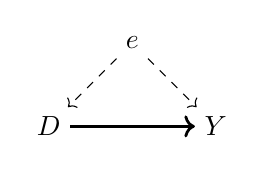
\begin{tikzpicture}
			[node distance=1.5cm]
		% nodes %
		\node[text centered] (e) {$e$};
		\node[below right of  = e, text centered] (y) {$Y$};
		\node[below left of = e, text centered] (d) {$D$};
 
		% edges %
		\draw[->, line width=1] (d) -- (y);
		\draw[dashed, ->] (e) -- (y);
		\draw[dashed, ->] (e) -- (d);
		\end{tikzpicture}
		\end{center}
		
		\begin{itemize}
		\item We are interested in the causal effect of juvenile incarceration ($D$) on life outcomes, like adult crime and high school completion
		\item But youth \emph{choose} to commit crimes, and that choice may be due to unobserved criminogenic factors like poverty or underlying criminal propensities which are themselves causing those future outcomes
		\end{itemize}
		

\end{frame}

\begin{frame}[plain]
\begin{center}
\textbf{Leniency as an instrument}
\end{center}

		\begin{center}
		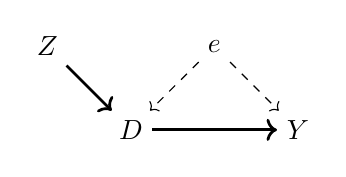
\begin{tikzpicture}
			[node distance=1.5cm]
		% nodes %
		\node[text centered] (e) {$e$};
		\node[below right of  = e, text centered] (y) {$Y$};
		\node[below left of = e, text centered] (d) {$D$};
		\node[above left of = d, text centered] (z) {$Z$};
 
		% edges %
		\draw[->, line width=1] (d) -- (y);
		\draw[->, line width=1] (z) -- (d);
		\draw[dashed, ->] (e) -- (y);
		\draw[dashed, ->] (e) -- (d);
		\end{tikzpicture}
		\end{center}
		
		\begin{itemize}
		\item Aizer and Doyle (2015) propose an instrument - the propensity to convict by the judge the youth is randomly assigned
		\item If judge assignment is random, and the various assumptions hold, then the IV strategy identifies the local average treatment effect of juvenile incarceration on life outcomes
		\end{itemize}

\end{frame}


\begin{frame}[plain]
\begin{center}
\textbf{The Main Idea}
\end{center}

	\begin{itemize}
	\item ``Plausibly exogenous'' variation in juvenile detention stemming from the random assignment of cases to judges who vary in their sentencing
	\item Consider two juveniles randomly assigned to two different judges with different incarceration tendencies (Scott and Bob)
	\item Random assignment ensures that differences in incarceration between Scott and Bob are due to the judge, not themselves, because remember, they're identical
	\end{itemize}
\end{frame}

\begin{frame}[plain]
\begin{center}
\textbf{Data}
\end{center}

	\begin{itemize}
	\item 35,000 juveniles administrative records over 10 years who came before a juvenile court in Chicago (Juvenile Court of Cook County Delinquency Database)
	\item Data were linked to public school data for Chicago (Chicago Public Schools) and adult incarceration data for Illinois (Illinois Dept. of Corrections Adult Admissions and Exits)
	\item They wanted to know the effect of juvenile incarceration on high school completion (2nd data needed) and adult crime (3rd data needed) using randomized judge assignment (1st data needed)
	\item They need personal identifying information in each data set to make this link (i.e., name, DOB, address)
	\end{itemize}
	
\end{frame}

\begin{frame}[plain]
\begin{center}
\textbf{Preview of findings}
\end{center}

	\begin{itemize}
	\item Juvenile incarceration decreased high school graduation by 13 percentage points (vs. 39pp in OLS)
	\item Increased adult incarceration by 23 percentage points (vs. 41pp in OLS)
	\item Marginal cases are high risk of adult incarceration and low risk of high school completion as a result of juvenile custody
	\item Unlikely to ever return to school after incarcerated, but when they do return, they are more likely to be classified as special ed students, and more likely to be classified for special ed services due to behavioral/emotional disorders (as opposed to cognitive disability)
	\end{itemize}
	
\end{frame}

\begin{frame}[plain]
\begin{center}
\textbf{``Plausibly'' exogenous}
\end{center}

	\begin{itemize}
	\item Very common in these studies for the assignment to some decision-maker to be \emph{arbitrary} but not clearly random (i.e., not random no. generator)
	\item In this case, juveniles charged with a crime are assigned to a calendar corresponding to their neighborhood and calendars have 1-2 judges who preside over them
	\item 1/5 of hearings are presided over by judges who cover the calendar when the main judge can't, known as swing judges
	\item Judge assignment is a function of the sequence with which cases happen to enter into the system and judge availability that is set in advance
	\item No scope for which judge you see first; conversations with court administrators confirm its random
	\end{itemize}
\end{frame}

\begin{frame}[plain]

\begin{center}
\textbf{Structural equation}
\end{center}

\begin{eqnarray*}
Y_i = \beta_0 + \beta_1 JI_i + \beta_2 X_i + \varepsilon_i
\end{eqnarray*}where $X_i$ is controls and $\varepsilon_i$ is an error term.  In this, juvenile incarceration is likely correlated with the error term.

\bigskip

This is the ``long'' causal model. But note, from the prior DAG, we cannot control for $e$ because it is unobserved. But it is confounding the estimation of juvenile incarceration's effect on outcomes.

\end{frame}

\begin{frame}[plain]
\begin{center}
\textbf{Incarceration Propensity as an Instrument}
\end{center}

	\begin{itemize}
	\item The instrument is based on the randomized judge equalling the propensity to incarcerate from the randomly assigned judge
	\item ``Leave-one-out mean''$$Z_{j(i)} = \bigg ( \frac{1}{n_{j(i)} - 1} \bigg ) \bigg ( \sum_{k \neq i}^{n_{j(i)}-1} \widetilde{JI}_k \bigg )$$
	\item The $n_{j(i)}$ terms is the total number of cases seen by judge $k$, and $\widetilde{JI}_k$ is equal to 1 if the juvenile was incarcerated during their first case
	\item Thus the instrument is the judge's incarceration among first cases based on all their other cases
	\item It's basically a judge fixed effect given the likelihood two judges have precisely the same propensity is small
	\end{itemize}
\end{frame}

\begin{frame}[plain]
\begin{center}
\textbf{Information about the instrument}
\end{center}

\begin{itemize}
	\item There are 62 judges in the data, and the average number of initial cases per judge is 607
	\item Substantial variation in the data - raw measure ranges from 4\% to 21\%
	\item Residualized measure based on controls still has substantial variation from 6\% to 18\%
	\item Variation comes from two sources: variation among the regular (nonswing) judges (80\% of cases) and variation from the swing judges (20\% of cases)
\end{itemize}

\end{frame}

\begin{frame}[plain]

	\begin{center}
	\textbf{Distribution of IV}
	\end{center}
	
	\begin{figure}
	\includegraphics[scale=0.15]{./lecture_includes/iv.png}
	\end{figure}
\end{frame}
	
\begin{frame}[plain]

	\begin{center}
	\textbf{Balance test}
	\end{center}
	
	\begin{figure}
	\includegraphics[scale=0.15]{./lecture_includes/balance.png}
	\end{figure}
\end{frame}

\begin{frame}[plain]

	\begin{center}
	\textbf{First stage}
	\end{center}
	
	\begin{figure}
	\includegraphics[scale=0.15]{./lecture_includes/firststage.png}
	\end{figure}
\end{frame}


\begin{frame}[plain]

	\begin{center}
	\textbf{High school completion}
	\end{center}
	
	\begin{figure}
	\includegraphics[scale=0.15]{./lecture_includes/highschool.png}
	\end{figure}
\end{frame}


\begin{frame}[plain]

	\begin{center}
	\textbf{Adult crime}
	\end{center}
	
	\begin{figure}
	\includegraphics[scale=0.2]{./lecture_includes/adult_crime.png}
	\end{figure}
\end{frame}


\begin{frame}[plain]

	\begin{center}
	\textbf{Crime type}
	\end{center}
	
	\begin{figure}
	\includegraphics[scale=0.2]{./lecture_includes/crimetype.png}
	\end{figure}
\end{frame}


\begin{frame}[plain]

	\begin{center}
	\textbf{High school transfers}
	\end{center}
	
	\begin{figure}
	\includegraphics[scale=0.2]{./lecture_includes/transfers.png}
	\end{figure}
\end{frame}


\begin{frame}[plain]

	\begin{center}
	\textbf{Developing emotional problems}
	\end{center}
	
	\begin{figure}
	\includegraphics[scale=0.2]{./lecture_includes/disorder.png}
	\end{figure}
\end{frame}


\begin{frame}[plain]

\begin{center}
\textbf{Concluding remarks}
\end{center}

	\begin{itemize}
	\item Sad, but important, paper - the marginal kid shouldn't have been incarcerated
	\item More generally, leniency designs are very powerful and very common if you know how to look for them
	\item Bottleneck, influential decision-makers, discretion - these are the three elements of the design
	\end{itemize}

\end{frame}


\begin{frame}[plain]
\begin{center}
\textbf{Comments on judge fixed effects}
\end{center}

\begin{itemize}
	\item Leave-one-out average propensity of the decision-maker, or some residualized instrument, is very common
	\item More often you'll see jackknife IV (JIVE) which drops observations while running regressions to improve finite sample bias
	\item The biggest threats aren't exclusion probably (though sometimes), but monotonicity
	\item Might judges be harsh in some situations (violent crimes) but lenient in others (female defendants, first time offenders)
\end{itemize}

\end{frame}

\begin{frame}[plain]
\begin{center}
\textbf{Tests for violations}
\end{center}

\begin{itemize}
\item New paper by Frandsen, Lefgren and Leslie (2019) proposes a test 
\item They show that the identifying assumptions imply a conditional expectation of the outcome of interest given the judge assignment is a continuous function of the judge propensity 
\item They propose a two-part test that generalizes the Sargan-Hansen over identification test and assesses whether treatment effects across judge propensities are possible 
\item Software available on Emily Leslie's website
\end{itemize}

\end{frame}

\begin{frame}[plain]
\begin{center}
\textbf{Multi-dimensional instrument}
\end{center}

\begin{itemize}
\item Peter Hull in a cautionary note notes that while combining judge fixed effects into a single propensity is numerically equivalent, it's still a series of dummies
\item Therefore it's very important to keep in mind the lessons we learned from weak instruments -- the more weak instruments you have when a parameter is overidentified, the larger the bias
\item It's ongoing at the moment to think about ways to improve instrument selection, but not settled
\item I encourage you to read Peter's note on his website and begin thinking about this yourself
\end{itemize}

\end{frame}


\begin{frame}[plain]
\begin{center}
\textbf{Discussion questions}
\end{center}

\begin{itemize}
\item When working on a judge fixed effects project, write down an IV DAG 
\item Whereas monotonicity cannot be visualized to my knowledge on a DAG, exclusion can -- so what does an exclusion violation mean in this context?
\item Use logic and conversations with those administering the program to answer the following -- what does monotonicity mean in this context and how might it be violated?  
\end{itemize}

\end{frame}


\begin{frame}[plain]
\begin{center}
\textbf{Empirical exercise}
\end{center}

\begin{itemize}

\item Let's estimate the effect of cash bail on defendant outcomes using 2SLS and JIVE
\item Excellent paper by Megan Stevenson
\item -\texttt{bail.do}- and -\texttt{bail.r}- in dropbox and github
\end{itemize}

\end{frame}




\section{Twoway fixed effects estimator}

\subsection{Introduction}

\begin{frame}
\begin{center}
\textbf{Twoway fixed effects}
\end{center}

\begin{itemize}
\item When working with panel data, the so-called ``twoway fixed effects'' (TWFE) estimator is the workhorse estimator
\item It's easy to run, a version of OLS, and many people are just interested in mean effects anyway
\item It's the most common model for estimating treatment effects in a difference-in-differences, and so for all these reasons, we need to spend some time understanding what it is
\end{itemize}

\end{frame}


\begin{frame}[plain]
	\begin{center}
	\textbf{Panel Data}
	\end{center}
	
	\begin{itemize}
	\item Panel data: we observe the same units (individuals, firms, countries, schools, etc.) over several time periods
	\item Often our outcome variable depends on unobserved factors which are also correlated with our explanatory variable of interest
	\item If these omitted variables are constant over time, we can use panel data estimators to consistently estimate the effect of our explanatory variable
	\end{itemize}
\end{frame}

\begin{frame}[plain]
\begin{center}
\textbf{What I will cover}
\end{center}

\begin{itemize}
		\item I will cover pooled OLS and twoway fixed effects
		\item But I won't be covering random effects, Arrelano and Bond and any number of important panel estimators because the purpose here is to present the modal regression model used in difference-in-differences
\end{itemize}

\end{frame}

\begin{frame}[plain]

	\begin{center}
	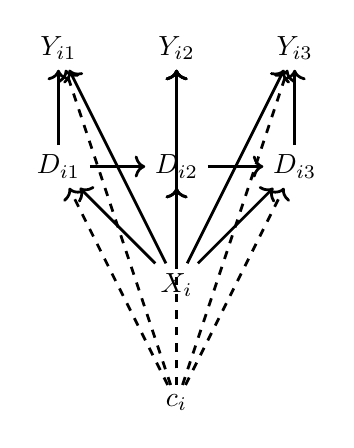
\begin{tikzpicture}
	[node distance=1.5cm]
	% nodes %
	\node[text centered] (y2) {$Y_{i2}$};
	\node[left of = y2, text centered] (y1) {$Y_{i1}$};
	\node[right of = y2, text centered] (y3) {$Y_{i3}$};
	\node[below of = y1, text centered] (d1) {$D_{i1}$};
	\node[below of = y2, text centered] (d2) {$D_{i2}$};
	\node[below of = y3, text centered] (d3) {$D_{i3}$};
	\node[below of = d2, text centered] (x) {$X_{i}$};
	\node[below of = x, text centered] (u) {$c_i$};
 
	% edges %
	\draw[->, line width= 1, ] (d1) -- (y1);
	\draw[->, line width= 1, ] (d2) -- (y2);
	\draw[->, line width= 1, ] (d3) -- (y3);
	\draw[->, line width= 1, ] (d1) -- (d2);
	\draw[->, line width= 1, ] (d2) -- (d3);
	\draw[->, line width= 1, dashed] (u) -- (d1);
	\draw[->, line width= 1, dashed] (u) -- (d2);
	\draw[->, line width= 1, dashed] (u) -- (d3);
	\draw[->, line width= 1, dashed] (u) -- (y1);
	\draw[->, line width= 1, dashed] (u) -- (y2);
	\draw[->, line width= 1, dashed] (u) -- (y3);
	\draw[->, line width= 1, ] (x) -- (d1);
	\draw[->, line width= 1, ] (x) -- (d2);
	\draw[->, line width= 1, ] (x) -- (d3);
	\draw[->, line width= 1, ] (x) -- (y1);
	\draw[->, line width= 1, ] (x) -- (y2);
	\draw[->, line width= 1, ] (x) -- (y3);
	\end{tikzpicture}
	\end{center}

Sorry - drawing the DAG for a simple panel model is somewhat messy!

\end{frame}


\begin{frame}[plain]
\begin{center}
\textbf{When to use this}
\end{center}

\begin{itemize}
\item Traditionally, this was used for estimating constant treatment effects with unobserved time-invariant heterogeneity -- recall the $c_i$ was constant across all time periods
\item It's a linear model, so you'll be estimating conditional mean treatment effects -- if you want the median, you can't use this
\item Once you enter into a world with dynamic treatment effects and differential timing, this loses all value
\end{itemize}

\end{frame}

\begin{frame}[plain]
	\begin{center}
	\textbf{Problems that fixed effects cannot solve}
	\end{center}
	
	\begin{itemize}
		\item Reverse causality: Becker predicted police reduce crime, but when you regress crime onto police, it's usually positive 
			\begin{itemize}
			\item $\widehat{\beta}_{FE}$ inconsistent unless strict exogeneity conditional on $c_i$ holds
				\begin{itemize}
				\item $E[\varepsilon_{it} | x_{i1},x_{i2},\dots,x_{iT},c_i]=0; t=1,2,\dots,T$
				\item implies $\varepsilon_{it}$ uncorrelated with past, current and future regressors
				\end{itemize}
			\end{itemize}
		\item Time-varying unobserved heterogeneity
			\begin{itemize}
			\item It's the time-varying unobservables you have to worry about in fixed effects
			\item Can include time-varying controls, but as always, don't condition on a collider
			\end{itemize}
	\end{itemize}
\end{frame}


\begin{frame}[plain]
	\begin{center}
	\textbf{Formal panel notation}
	\end{center}
	
	\begin{itemize}
	\item Let $y$ and $x\equiv(x_1, x_2, \dots, x_k)$ be observable random variables and $c$ be an unobservable random variable
	\item We are interested in the partial effects of variable $x_j$ in the population regression function$$E[y|x_1,x_2,\dots,x_k,c]$$
	\end{itemize}
\end{frame}

\begin{frame}[plain]
\begin{center}
\textbf{Formal panel notation cont.}
\end{center}

\begin{itemize}
	\item We observe a sample of $i=1,2,\dots,N$ cross-sectional units for $t=1,2,\dots,T$ time periods (a balanced panel)
		\begin{itemize}
		\item For each unit $i$, we denote the observable variables for all time periods as $\{(y_{it},x_{it}):t=1,2,\dots,T\}$
		\item $x_{it}\equiv(x_{it1},x_{it2}, \dots, x_{itk})$ is a $1\times K$ vector
		\end{itemize}
	\item Typically assume that cross-sectional units are i.i.d. draws from the population: $\{y_i, x_i, c_i\}^N_{i=1}\sim i.i.d.$ (cross-sectional independence)
		\begin{itemize}
		\item $y_i \equiv (y_{i1}, y_{i2}, \dots, y_{iT})'$ and $x_i \equiv (x_{i1},x_{i2}, \dots, x_{iT})$
		\item Consider asymptotic properties with $T$ fixed and $N\rightarrow \infty$
		\end{itemize}
\end{itemize}

\end{frame}

\begin{frame}[plain]
	\begin{center}
	\textbf{Formal panel notation}
	\end{center}
Single unit:

\[ y_i = \left( \begin{array}{c}
y_{i1} \\
\vdots \\
y_{it} \\
\vdots \\
y_{iT}
\end{array} \right)_{T\times 1}
%
X_i = \left( \begin{array}{ccccc}
X_{i,1,1} & X_{i,1,2} & X_{i,1,j} & \dots & X_{i,1,K} \\
\vdots & \vdots & \vdots & & \vdots \\
X_{i,t,1} & X_{i,t,2} & X_{i,t,j} & \dots & X_{i,t,K} \\
\vdots & \vdots & \vdots & & \vdots \\
X_{i,T,1} & X_{i,T,2} & X_{i,T,j} & \dots & X_{i,T,K} 
\end{array} \right)_{T\times K}
\]

Panel with all units:
\[ y = \left( \begin{array}{c}
y_{1} \\
\vdots \\
y_{i} \\
\vdots \\
y_{N}
\end{array} \right)_{NT\times 1}
%
X = \left( \begin{array}{c}
X_1  \\
\vdots \\
X_i \\
\vdots \\
X_N
\end{array} \right)_{NT \times K}
\]


\end{frame}

\begin{frame}[plain]
	\begin{center}
	\textbf{Unobserved heterogeneity}
	\end{center}
	
	\begin{itemize}
	\item For a randomly drawn cross-sectional unit $i$, the model is given by $$y_{it} = x_{it}\beta + c_i + \varepsilon_{it}, \text{   }t=1,2,\dots,T$$
		\begin{itemize}
		\item $y_{it}$: log wages $i$ in year $t$
		\item $x_{it}:1 \times K$ vector of variable events for person $i$ in year $t$, such as education, marriage, etc. plus an intercept
		\item $\beta: K\times 1$ vector of marginal effects of events
		\item $c_i$: sum of all time-invariant inputs known to people $i$ (but unobserved for the researcher), e.g., ability, beauty, grit, etc., often called unobserved heterogeneity or fixed effect
		\item $\varepsilon_{it}$: time-varying unobserved factors, such as a recession, unknown to the farmer at the time the decision on the events $x_{it}$ are made, sometimes called idiosyncratic error
		\end{itemize}
	\end{itemize}
\end{frame}

\subsection{Two Estimators}

\begin{frame}
\begin{center}
\textbf{Pooled OLS}
\end{center}

\begin{itemize}
	\item When we ignore the panel structure and regress $y_{it}$ on $x_{it}$ we get$$ y_{it}=x_{it}\beta + v_{it}; \text{    }t=1,2,\dots,T$$with composite error $v_{it} \equiv c_i + \varepsilon_{it}$
	\item What happens when we regress $y_{it}$ on $x_{it}$ if $x$ is correlated with $c_i$?
	\item Then $x$ ends up correlated with $v$, the composite error term.
	\item Somehow we need to eliminate this bias, but how?
\end{itemize}

\end{frame}

\begin{frame}[plain]
	\begin{center}
	\textbf{Pooled OLS}
	\end{center}
	
	\begin{itemize}
	\item Main assumption to obtain consistent estimates for $\beta$ is:
		\begin{itemize}
		\item $E[v_{it} | x_{i1},x_{i2}, \dots, x_{iT}] = E[v_{it} | x_{it}] = 0$ for $t=1,2,\dots, T$
			\begin{itemize}
			\item $x_{it}$ are strictly exogenous: the composite error $v_{it}$ in each time period is uncorrelated with the past, current and future regressors
			\item But: education $x_{it}$ likely depends on grit and ability $c_i$ and so we have omitted variable bias and $\widehat{\beta}$ is not consistent
			\end{itemize}
		\item No correlation between $x_{it}$ and $v_{it}$ implies no correlation between unobserved effect $c_i$ and $x_{it}$ for all $t$
			\begin{itemize}
			\item Violations are common: whenever we omit a time-constant variable that is correlated with the regressors (heterogeneity bias)
			\end{itemize}
		\item Additional problem: $v_{it}$ are serially correlated for same $i$ since $c_i$ is present in each $t$ and thus pooled OLS standard errors are invalid
		\end{itemize}
	\end{itemize}
\end{frame}

\begin{frame}[plain]
	\begin{center}
	\textbf{Pooled OLS}
	\end{center}
	
	\begin{itemize}
	\item Always ask: is there a time-constant unobserved variable ($c_i$) that is correlated with the regressors?  
	\item If yes, then pooled OLS is problematic
	\item This is how we motivate a fixed effects model: because we believe unobserved heterogeneity is the main driving force making the treatment variable endogenous
	\end{itemize}
\end{frame}

\begin{frame}[plain]
	\begin{center}
	\textbf{Fixed effect regression}
	\end{center}
	
	\begin{itemize}
	\item Our unobserved effects model is:$$y_{it} = x_{it}\beta + c_i + \varepsilon_{it}; t=1,2,\dots,T$$
	\item If we have data on multiple time periods, we can think of $c_i$ as \textbf{fixed effects} to be estimated
	\item OLS estimation with fixed effects yields$$(\widehat{\beta}, \widehat{c}_1, \dots, \widehat{c}_N) = \underset{b,m_1,\dots,m_N}{\arg\!\min} \sum_{i=1}^N\sum_{t=1}^T (y_{it} - x_{it}b - m_i)^2$$this amounts to including $N$ individual dummies in regression of $y_{it}$ on $x_{it}$
	\end{itemize}
\end{frame}

\begin{frame}[plain]
	\begin{center}
	\textbf{Derivation: fixed effects regression}
	\end{center}
	
$$(\widehat{\beta}, \widehat{c}_1, \dots, \widehat{c}_N) = \underset{b,m_1,\dots,m_N}{\arg\!\min} \sum_{i=1}^N\sum_{t=1}^T (y_{it} - x_{it}b - m_i)^2$$

The first-order conditions (FOC) for this minimization problem are: $$\sum_{i=1}^N \sum_{t=1}^T x_{it}'(y_{it} - x_{it}\widehat{\beta} - \widehat{c}_i)=0$$ and $$\sum_{t=1}^T(y_{it} - x_{it}\widehat{\beta} - \widehat{c}_i) = 0 $$ for $i=1,\dots,N$.
	
\end{frame}

\begin{frame}[shrink=20,plain]
	\begin{center}
	\textbf{Derivation: fixed effects regression}
	\end{center}
	
Therefore, for $i=1, \dots, N$,$$\widehat{c}_i = \frac{1}{T} \sum_{t=1}^T(y_{it}-x_{it}\widehat{\beta})=\bar{y}_i-\bar{x}_i\widehat{\beta},$$where$$\bar{x}_i \equiv \frac{1}{T}\sum_{t=1}^Tx_{it}; \bar{y}_i \equiv \frac{1}{T} \sum_{t=1}^T y_{it}$$
Plug this result into the first FOC to obtain:$$\widehat{\beta} = \bigg( \sum_{i=1}^N \sum_{t=1}^T (x_{it} - \bar{x}_i)'(x_{it} - \bar{x}_i) \bigg)^{-1} \bigg( \sum_{i=1}^N \sum_{t=1}^T (x_{it} - \bar{x}_i)'(y_{it} - \bar{y})\bigg)$$ $$\widehat{\beta} = \bigg(\sum_{i=1}^N \sum_{t=1}^T \ddot{x}_{it}'\ddot{x}_{it} \bigg)^{-1} \bigg( \sum_{i=1}^N \sum_{t=1}^T \ddot{x}_{it}' \ddot{x}_{it} \bigg)$$
with time-demeaned variables $\ddot{x}_{it} \equiv x_{it}-\bar{x},\ddot{y}_{it} \equiv y_{it} - \bar{y}_i$
\end{frame}

\begin{frame}[plain]
	\begin{center}
	\textbf{Fixed effects regression}
	\end{center}
	
Running a regression with the time-demeaned variables $\ddot{y}_{it}\equiv y_{it} - \bar{y}_i$ and $\ddot{x}_{it} \equiv x_{it} - \bar{x}$ is numerically equivalent to a regression of $y_{it}$ on $x_{it}$ and unit specific dummy variables.

\vspace{10mm}

Even better, the regression with the time demeaned variables is consistent for $\beta$ even when $Cov[x_{it},c_i]\neq 0$ because time-demeaning eliminates the unobserved effects

\begin{eqnarray*}
y_{it} &=& x_{it}\beta + c_i + \varepsilon_{it} \\
\bar{y}_i &=& \bar{x}_i \beta + c_i + \bar{\varepsilon}_{i}\\
\hline \\
(y_{it} - \bar{y}_i) &=& (x_{it} - \bar{x})\beta + (c_i - c_i) + (\varepsilon_{it} - \bar{\varepsilon}_i) \\
\ddot{y}_{it} &=& \ddot{x}_{it}\beta + \ddot{\varepsilon}_{it}
\end{eqnarray*}

\end{frame}

\begin{frame}[plain]
	\begin{center}
	\textbf{Fixed effects regression: main results}
	\end{center}
	
	\begin{itemize}
	\item Identification assumptions:	
		\begin{enumerate}
		\item $E[\varepsilon_{it} | x_{i1}, x+{i2}, \dots, x_{iT}, c_i]=0; t=1,2,\dots,T$
			\begin{itemize}
			\item regressors are strictly exogenous conditional on the unobserved effect
			\item allows $x_{it}$ to be arbitrarily related to $c_i$
			\end{itemize}
		\item $rank\bigg( \sum_{t=1}^T E[\ddot{x}_{it}'\ddot{x}_{it}]\bigg) = K$
			\begin{itemize}
			\item regressors vary over time for at least some $i$ and not collinear
			\end{itemize}
		\end{enumerate}
	\item Fixed effects estimator
		\begin{enumerate}
		\item Demean and regress $\ddot{y}_{it}$ on $\ddot{x}_{it}$ (need to correct degrees of freedom)
		\item Regress $y_{it}$ on $x_{it}$ and unit dummies (dummy variable regression)
		\item Regress $y_{it}$ on $x_{it}$ with canned fixed effects routine
			\begin{itemize}
			\item Stata: \texttt{xtreg y x, fe i(PanelID)}
			\end{itemize}
		\end{enumerate}
	\end{itemize}
\end{frame}


\begin{frame}[plain]
\begin{center}
\textbf{FE main results}
\end{center}

\begin{itemize}
	\item Properties (under assumptions 1-2):
		\begin{itemize}
		\item $\widehat{\beta}_{FE}$ is consistent: $\underset{N\rightarrow \infty}{plim} \widehat{\beta}_{FE,N}=\beta$
		\item $\widehat{\beta}_{FE}$ is unbiased conditional on \textbf{X}
		\end{itemize}
\end{itemize}

\end{frame}

\begin{frame}[plain]
	\begin{center}
	\textbf{Fixed effects regression: main issues}
	\end{center}
	
	\begin{itemize}
	\item Inference:
		\begin{itemize}
		\item Standard errors have to be ``clustered'' by panel unit (e.g., farm) to allow correlation in the $\varepsilon_{it}$'s for the same $i$.
		\item Yields valid inference as long as number of clusters is reasonably large
		\end{itemize}	
	\item Typically we care about $\beta$, but unit fixed effects $c_i$ could be of interest
		\begin{itemize}
		\item $\widehat{c}_i$ from dummy variable regression is unbiased but not consistent for $c_i$ (based on fixed $T$ and $N\rightarrow \infty$)
		\end{itemize}
	\end{itemize}
\end{frame}

\subsection{Empirical exercise}

\begin{frame}
\begin{center}
\textbf{Application: SASP}
\end{center}

\begin{itemize}
\item From 2008-2009, I fielded a survey of Internet sex workers (685 respondents, 5\% response rate)
\item I asked two types of questions: static provider-specific information (e.g., age, weight) and dynamic session information over last 5 sessions
\item Let's look at the panel aspect of this analysis together
\end{itemize}

\end{frame}

\begin{frame}[plain]
\begin{center}
\textbf{Risk premium equation}
\end{center}

\begin{eqnarray*}
Y_{is} &=& \beta_i X_i + \delta{D_{is}} + \gamma_{is} Z_{is} + u_i + \varepsilon_{is} \\
\ddot{Y}_{is} &=& \gamma_{is} \ddot{Z}_{is} + \ddot \eta_{is}
\end{eqnarray*}where $Y$ is log price, $D$ is unprotected sex with a client in a session,  $X$ are client and session characteristics, $Z$ is unobserved heterogeneity, and $u_i$ is both unobserved and correlated with $Z_{is}$.  

\end{frame}

\begin{frame}[plain]
\begin{table}[htbp]\centering
\tiny
\caption{POLS, FE and Demeaned OLS Estimates of the Determinants of Log Hourly Price for a Panel of Sex Workers}
\label{sasp}
\begin{center}
\begin{threeparttable}
\begin{tabular}{l*{3}{c}}
\toprule
\multicolumn{1}{l}{\textbf{Depvar:}}&
\multicolumn{1}{c}{\textbf{POLS}}&
\multicolumn{1}{c}{\textbf{FE}}&
\multicolumn{1}{c}{\textbf{Demeaned OLS}}\\
\midrule
Unprotected sex with client of any kind					&       0.013   &       0.051*  &       0.051* \\
                    									&     (0.028)   &     (0.028)   &     (0.026) \\
Ln(Length)          									&      -0.308***&      -0.435***&      -0.435*** \\
                    									&     (0.028)   &     (0.024)   &     (0.019) \\
Client was a Regular									&      -0.047*  &      -0.037** &      -0.037** \\
                    									&     (0.028)   &     (0.019)   &     (0.017) \\
Age of Client       									&      -0.001   &       0.002   &       0.002 \\
                    									&     (0.009)   &     (0.007)   &     (0.006) \\
Age of Client Squared									&       0.000   &      -0.000   &      -0.000 \\
                    									&     (0.000)   &     (0.000)   &     (0.000) \\
Client Attractiveness (Scale of 1 to 10)				&       0.020***&       0.006   &       0.006 \\
                    									&     (0.007)   &     (0.006)   &     (0.005) \\
Second Provider Involved								&       0.055   &       0.113*  &       0.113* \\
                    									&     (0.067)   &     (0.060)   &     (0.048) \\
Asian Client        									&      -0.014   &      -0.010   &      -0.010 \\
                    									&     (0.049)   &     (0.034)   &     (0.030) \\
Black Client        									&       0.092   &       0.027   &       0.027 \\
                    									&     (0.073)   &     (0.042)   &     (0.037) \\
Hispanic Client     									&       0.052   &      -0.062   &      -0.062 \\
                    									&     (0.080)   &     (0.052)   &     (0.045) \\
Other Ethnicity Client									&       0.156** &       0.142***&       0.142*** \\
                    									&     (0.068)   &     (0.049)   &     (0.045) \\
Met Client in Hotel 									&       0.133***&       0.052*  &       0.052* \\
                    									&     (0.029)   &     (0.027)   &     (0.024) \\
Gave Client a Massage									&      -0.134***&      -0.001   &      -0.001 \\
                    									&     (0.029)   &     (0.028)   &     (0.024) \\
Age of provider     									&       0.003   &       0.000   &       0.000 \\
                    									&     (0.012)   &         (.)   &         (.) \\
Age of provider squared									&      -0.000   &       0.000   &       0.000 \\
                    									&     (0.000)   &         (.)   &         (.) \\
\end{tabular}
\end{threeparttable}
\end{center}
\end{table}

\end{frame}


\begin{frame}[plain]
\begin{table}[htbp]\centering
\tiny
\caption{POLS, FE and Demeaned OLS Estimates of the Determinants of Log Hourly Price for a Panel of Sex Workers}
\label{sasp}
\begin{center}
\begin{threeparttable}
\begin{tabular}{l*{3}{c}}
\toprule
\multicolumn{1}{l}{\textbf{Depvar:}}&
\multicolumn{1}{c}{\textbf{POLS}}&
\multicolumn{1}{c}{\textbf{FE}}&
\multicolumn{1}{c}{\textbf{Demeaned OLS}}\\
\midrule
Body Mass Index     									&      -0.022***&       0.000   &       0.000 \\
                    									&     (0.002)   &         (.)   &         (.) \\
Hispanic   									&      -0.226***&       0.000   &       0.000 \\
                    									&     (0.082)   &         (.)   &         (.) \\
Black      									&       0.028   &       0.000   &       0.000 \\
                    									&     (0.064)   &         (.)   &         (.) \\
 Other      									&      -0.112   &       0.000   &       0.000 \\
                    									&     (0.077)   &         (.)   &         (.) \\
 Asian      									&       0.086   &       0.000   &       0.000 \\
                    									&     (0.158)   &         (.)   &         (.) \\
Imputed Years of Schooling								&       0.020** &       0.000   &       0.000 \\
                   	 									&     (0.010)   &         (.)   &         (.) \\
Cohabitating (living with a partner) but unmarried	&      -0.054   &       0.000   &       0.000 \\
                    									&     (0.036)   &         (.)   &         (.) \\
Currently married and living with your spouse		&       0.005   &       0.000   &       0.000 \\
                    									&     (0.043)   &         (.)   &         (.) \\
Divorced and not remarried							&      -0.021   &       0.000   &       0.000 \\
                    									&     (0.038)   &         (.)   &         (.) \\
Married but not currently living with your spouse	&      -0.056   &       0.000   &       0.000 \\
                    									&     (0.059)   &         (.)   &         (.) \\
\\
N                   									&       1,028   &       1,028   &       1,028\\
Mean of dependent variable								&        5.57   &        5.57   &        0.00\\
\bottomrule
\end{tabular}
\begin{tablenotes}
\tiny
\item Heteroskedastic robust standard errors in parenthesis clustered at the provider level. * p$<$0.10, ** p$<$0.05, *** p$<$0.01
\end{tablenotes}
\end{threeparttable}
\end{center}
\end{table}

\end{frame}




\begin{frame}[plain]
	\begin{center}
	\textbf{Unit specific time trends often eliminate ``results''}
	\end{center}
	
\begin{table}[htbp]\centering
\tiny
\caption{Demeaned OLS Estimates of the Determinants of Log Hourly Price for a Panel of Sex Workers with provider specific trends}
\label{sasp}
\begin{center}
\begin{threeparttable}
\begin{tabular}{l*{1}{c}}
\toprule
\multicolumn{1}{l}{\textbf{Depvar:}}&
\multicolumn{1}{c}{\textbf{FE w/provider trends}}\\
\midrule
Unprotected sex with client of any kind&       0.004   \\
                    &     (0.046)   \\
Ln(Length)          &      -0.450***\\
                    &     (0.020)   \\
Client was a Regular&      -0.071** \\
                    &     (0.023)   \\
Age of Client       &       0.008   \\
                    &     (0.005)   \\
Age of Client Squared&      -0.000   \\
                    &     (0.000)   \\
Client Attractiveness (Scale of 1 to 10)&       0.003   \\
                    &     (0.003)   \\
Second Provider Involved&       0.126*  \\
                    &     (0.055)   \\
Asian Client        &      -0.048***\\
                    &     (0.007)   \\
Black Client        &       0.017   \\
                    &     (0.043)   \\
Hispanic Client     &      -0.015   \\
                    &     (0.022)   \\
Other Ethnicity Client&       0.135***\\
                    &     (0.031)   \\
Met Client in Hotel &       0.073***\\
                    &     (0.019)   \\
Gave Client a Massage&       0.022   \\
                    &     (0.012)   \\
\end{tabular}
\end{threeparttable}
\end{center}
\end{table}

	
 	
\end{frame}

\begin{frame}[plain]
\begin{center}
\textbf{Concluding remarks}
\end{center}

\begin{itemize}
\item This is not a review of panel econometrics; for that see Wooldridge and other excellent options
\item We reviewed POLS and TWFE because they are commonly used with individual level panel data and difference-in-differences
\item Their main value is how they control for unobserved heterogeneity through a simple demeaning
\item Now let's discuss difference-in-differences which will at various times use the TWFE model
\end{itemize}

\end{frame}

\section{Differences-in-differences}

\subsection{John Snow}

\begin{frame}
\begin{center}
\textbf{John Snow}
\end{center}

\begin{itemize}
\item John Snow was a practicing anesthesiologist in the mid 19th century London
\item He was then famous for inventing a machine that would carefully deliver chloroform to patients in homogenous dosage which reduced mortality from anasthesia
\item But he is now famous for providing convincing evidence that cholera was a waterborne disease during the 1854 outbreak
\item Published two works on cholera -- an essay in 1849, and a book in 1855
\item Died of a stroke in 1858
\end{itemize}

\end{frame}


\begin{frame}[plain]

\begin{figure}
\includegraphics[scale=0.2]{./lecture_includes/cholera.png}
\caption{Daily cholera deaths, London (Coleman 2019)}
\end{figure}

\end{frame}

\begin{frame}[plain]
\begin{center}
\textbf{Cholera background}
\end{center}

\begin{itemize}
\item Cholera hits London three times in the early to mid 1800s causing large waves of tens of thousands of deaths
\item Three London epidemics -- 1831-1832, 1848-1849, 1853-1854
\item Cholera attacked victims suddenly, with a 50\% survival rate, and very painful symptoms included vomiting and acute diarrhea
\end{itemize}

\end{frame}


\begin{frame}[plain]
\begin{center}
\textbf{Miasmis}
\end{center}

\begin{itemize}
\item 19th century London was a filthy place with waste collecting in cesspools under houses or emptied into open ditches and sewers
\item Majority opinion about disease was \emph{miasmis}
\item Miasmis hypothesized that disease transmission was caused by vapors and smells; unclear its relevance for person-to-person 
\end{itemize}

\end{frame}

\begin{frame}[plain]
\begin{center}
\textbf{Never before seen microorganism}
\end{center}

\begin{itemize}
\item Microscopes were around but had horrible resolution
\item Most human pathogens couldn't be seen
\item Johnson (2007) reports Snow did track down a microscope but could only see blurry things moving around
\item Isolating these microorganisms wouldn't occur for half a century
\end{itemize}

\end{frame}



\begin{frame}[plain]
\begin{center}
\textbf{Snow's hypothesis}
\end{center}

\begin{itemize}
	\item Snow (as well as a few others like Rev. Henry Whitehead) believe miasmis is not relevant for explaining cholera
	\item Snow hypothesizes that the active agent was a living organism that entered the body, got into the alimentary canal with food or drink, multiplied in the body, and generated some poison that caused the body to expel water
	\item The organism passed out of the body with these evacuations, entered the water supply and infected new victims
	\item The process repeated itself, growing rapidly through the common water supply, causing an epidemic

\end{itemize}

\end{frame}

\begin{frame}[plain]
\begin{center}
\textbf{Thought Experiment}
\end{center}

\begin{itemize}
\item How will he convince anyone that cholera is waterborne and not due to ``bad air''?  
\item Consider the ideal experiment: randomize households by coin flip to receive water from runoff (control) vs. water without runoff (treatment)
\item Unethical, impractical and unrealistic
\item Even if the randomized experiment is not possible, the thought experiment suggests the observational equivalent
\end{itemize}

\end{frame}


\begin{frame}[plain]
\begin{center}
\textbf{Multiple sources of evidence, not just one}
\end{center}

Snow makes his argument with many pieces of evidence that when taken together are very compelling that water, not air, is the cause of the cholera epidemics. These can be categorized as:
\begin{enumerate}
\item Observation
\item Broad Street Pump
\item Grand Experiment
\end{enumerate}

\end{frame}


\begin{frame}[plain]
\begin{center}
\textbf{Observation}
\end{center}

\begin{itemize}
\item Observed progression of the disease for years
\item Tracked Patient Zero 
\item Treatments didn't work:  Snow would cover with burlap sacks, which did nothing
\item Strange irregular patterns -- higher deaths in close proximity to a public pump on Broad Street, fewer deaths at a pub
\end{itemize}
\begin{quote}
``cholera extended to nearly all the houses in which the water was thus tainted, and to no others.'' (Snow 1849)
\end{quote}
\end{frame}

\begin{frame}[plain]
\begin{center}
\textbf{Broad street outbreak}
\end{center}

\begin{quote}
``The most terrible outbreak of cholera which ever occurred in this kingdom, is probably that
which took place in Broad Street, Golden Square, and the adjoining streets, a few weeks ago. Within two
hundred and fifty yards of the spot where Cambridge Street [now Lexington St.] joins Broad Street [now
Broadwick], there were upwards of five hundred fatal attacks of cholera in ten days.'' (Snow 1855)
\end{quote}
\end{frame}

\begin{frame}[plain]
\begin{center}
\textbf{How he argues for the Broad street pump}
\end{center}

\begin{itemize}
\item Famous map showing unusual mass of cholera deaths near the public Broad street pump
\item He was looking for the source, but he was not inductively forming his theory with this map because he already knew the mechanism
\item He was assembling evidence that would further refute the explanations of those who advocated an alternative explanation of the outbreak
\end{itemize}

\end{frame}

\begin{frame}[plain]

\begin{figure}
\includegraphics[scale=0.08]{./lecture_includes/Snow-cholera-map-1.jpeg}
\caption{Cholera deaths laid over a small area of London near Broad Street}
\end{figure}

\end{frame}

\begin{frame}[plain]
\begin{center}
\textbf{Map was important but not enough on its own}
\end{center}

\begin{quote}
``[Snow] could see at a glance that he'd be able to demonstrate that the outbreak was clustered
around the pump, yet he knew from experience that that kind of evidence, on its own, would
not satisfy a miasmatist. The cluster could just as easily reflect some pocket of poisoned air that
had settled over that part of Soho, something emanating from the gulley holes or cesspools -- or
perhaps even from the pump itself. Snow knew that the case would be made in the exceptions
from the norm. Pockets of life where you could expect death, pockets of death where you would
expect life.'' Johnson (2007) p. 140
\end{quote}

\end{frame}

\begin{frame}[plain]
\begin{center}
\textbf{Two companies fight for customers}
\end{center}

\begin{itemize}
\item Southwark and Vauxhall Waterworks Company and the Lambeth Water Company competed over some of the regions south of the Thames
\item In 16 sub-districts, with a population of 300,000, they competed directly, even supplying customers side-by-side
\end{itemize}

\begin{quote}
``In many cases a single house has a supply different from that on either side. Each company
supplies both rich and poor, both large houses and small; there is no difference in the condition
or occupation of the persons receiving the water of the different companies.'' Snow (1855) p 75
\end{quote}

\end{frame}



\begin{frame}[plain]
\begin{center}
\textbf{Lambeth moves its pipe}
\end{center}

\begin{itemize}
\item During the 1849 epidemic, both companies drew water from Thames which was polluted with sewage and cholera
\item London passes legislation requiring utility companies to move their pipes above the city
\item In 1852, the Lambeth Company, a water utility company, changed supply from Hungerford Bridge
\item It moved its intake pipe upstream to cleaner water and in response to legislation (SV delayed)
\item This created a natural experiment because Southwark and Vauxhall left its intake pipe in place
\end{itemize}

\end{frame}



\begin{frame}[plain]
\begin{center}
\textbf{Meticulous Data Collection}
\end{center}

\begin{itemize}
\item Two types of data: DD uses aggregate deaths bc of mixing of customers whereas his Broad Street evidence focused on individuals
\item Collected detailed information from households with cholera deaths on utility subscription (Lambeth or SV)
\item Many residents didn't know their water company -- distant landlords paid for it
\item He knew Lambeth water was four times saltier, so he'd take a sample and test it using a saline test back at his office
\end{itemize}

\end{frame}


\begin{frame}[plain]
\begin{center}
\textbf{Shoeleather and knowledge of institutional details}
\end{center}

\begin{itemize}
\item Careful balance checks -- ``the pipes of each Company go down all the streets into nearly all the courts and alleys''
\item Concern for sample selection bias --``No fewer than 3000 people of both sexes [of all types affected]''
\item Treatment assignment was arbitrary -- ``a few houses supplied by one Company and a few by the other''
\end{itemize}

\end{frame}

\begin{frame}[plain]

\begin{center}
\textbf{Table XII}
\end{center}

\begin{center}
\begin{large}Modified Table XII (Snow 1854) \end{large}
\footnotesize
\begin{tabular}{lcc}
\toprule
\multicolumn{1}{c}{\textbf{Company name}}&
\multicolumn{1}{c}{\textbf{1849}}&
\multicolumn{1}{c}{\textbf{1854}} \\
\midrule
Southwark and Vauxhall & 135 & 147\\
Lambeth	& 85 & 19 \\
\bottomrule
\end{tabular}
\end{center}

Estimated ATT using DD is 78 fewer deaths per 10,000

\end{frame}

\begin{frame}[plain]
\begin{center}
\textbf{Failure to convince}
\end{center}

\begin{quote}
``In spite of what has since been recognized as a classic exercise in data, analysis, and argument, Snow failed to convince the medical profession, the policy-making establishment, or the public.'' (Coleman 2019)
\end{quote}

\end{frame}

\begin{frame}[plain]
\begin{center}
\textbf{Final victory}
\end{center}

\begin{itemize}
\item Another cholera outbreak in 1866, east of London, is when Snow's ideas were gradually and reluctantly accepted by public officials and the scientific community
\item 1866 outbreak was confined only to the east of London, which was the last area not yet connected to the newly constructed sewage system which discharged sewage below the Thames
\item The rest of London didn't have an outbreak
\item This was the final piece of evidence that swayed skeptics and led to a more reasoned assessment of Snow's data and analysis
\end{itemize}

\end{frame}

\begin{frame}[plain]
\begin{center}
\textbf{Merits of Snow's work}
\end{center}

\begin{itemize}
\item Long commitment to the topic led him to reject unsound hypotheses and form new ones based on observation and experience (shoe leather)
\item Expert handling of data analysis, data visualization, and a framing of evidence with a ladder of reasoning
\end{itemize}

\end{frame}

%\begin{frame}[plain]
%\begin{center}
%\textbf{Shoe leather}
%\end{center}

%\begin{quote}``The force of [Snow's] argument results from the clarity of the prior reasoning, the bringing together of many different lines of evidence, and the amount of shoe leather Snow was willing to use to get the data.   Snow did some brilliant detective work on nonexperimental data.  What is impressive is not the statistical technique but the handling of the scientific issues.  He made steady progress from shrewd observation through case studies to analyze ecological data.  In the end, he found and analyzed a natural experiment.'' (Freedman 1991)
%\end{quote}

%\end{frame}

\begin{frame}[plain]
\begin{center}
\textbf{Layered rhetoric of research}
\end{center}

\begin{quote}
``The strength of his model derived from its ability to use observed phenomena on one scale to make predictions about behavior on other scales up and down the chain. ... If cholera were waterborne then the patterns of infection must correlate with the patterns of water distribution in London's neighborhoods. Snow?s theory was like a ladder; each individual rung was impressive enough, but the power of it lay in ascending from bottom to top, from the membrane of the small intestine all the way up to the city itself.'' (Johnson, Ghost Map)
\end{quote}

\end{frame}


\subsection{The simple 2x2}


\begin{frame}
\begin{center}
\textbf{Simple cross-sectional design}
\end{center}

\begin{table}\centering
		\caption{Lambeth and Southwark and Vauxhall, 1854}
		\begin{center}
		\begin{tabular}{ll}
		\toprule
		\multicolumn{1}{l}{\textbf{Company}}&
		\multicolumn{1}{c}{\textbf{Cholera mortality}}\\
		\midrule
		Lambeth  & $Y=L + D$ \\
		\midrule
		Southwark and Vauxhall  & $Y=SV$ \\
		\bottomrule
		\end{tabular}
		\end{center}
	\end{table}

\end{frame}

\begin{frame}[plain]
\begin{center}
\textbf{Interrupted time series design}
\end{center}

	\begin{table}\centering
		\caption{Lambeth, 1849 and 1854}
		\begin{center}
		\begin{tabular}{lll}
		\toprule
		\multicolumn{1}{l}{\textbf{Company}}&
		\multicolumn{1}{c}{\textbf{Time}}&
		\multicolumn{1}{c}{\textbf{Cholera mortality}}\\
		\midrule
		Lambeth & 1854 & $Y=L$ \\
		& 1849 & $Y=L + (T + D)$ \\
		\bottomrule
		\end{tabular}
		\end{center}
	\end{table}

\end{frame}

\begin{frame}[plain]
\begin{center}
\textbf{Difference-in-differences}
\end{center}

\begin{table}\centering
		\caption{Lambeth and Southwark and Vauxhall, 1849 and 1854}
		\begin{center}
		\begin{tabular}{lll|lc}
		\toprule
		\multicolumn{1}{l}{\textbf{Companies}}&
		\multicolumn{1}{c}{\textbf{Time}}&
		\multicolumn{1}{c}{\textbf{Outcome}}&
		\multicolumn{1}{c}{$D_1$}&
		\multicolumn{1}{c}{$D_2$}\\
		\midrule
		Lambeth & Before & $Y=L$ \\
		& After & $Y=L + T + D$ & $T+D$\\
		\midrule
		& & & & $D$ \\
		\midrule
		Southwark and Vauxhall & Before & $Y=SV$ \\
		& After & $Y=SV + T$ & $T$\\
		\bottomrule
		\end{tabular}
		\end{center}
	\end{table}

\end{frame}




\begin{frame}[plain]
\begin{center}
\textbf{Sample averages}
\end{center}

\begin{eqnarray*}
\widehat{\delta}^{2x2}_{kU} = \bigg ( \overline{y}_k^{post(k)} - \overline{y}_k^{pre(k)} \bigg ) - \bigg ( \overline{y}_U^{post(k)} - \overline{y}_U^{pre(k)} \bigg )
\end{eqnarray*}

\end{frame}

\begin{frame}[plain]
\begin{center}
\textbf{Population expectations}
\end{center}

\begin{eqnarray*}
\widehat{\delta}^{2x2}_{kU} = \bigg ( E[Y_k|Post] - E[Y_k|Pre] \bigg ) - \bigg ( E[Y_U | Post ] - E[ Y_U | Pre] \bigg) \\
\end{eqnarray*}

\end{frame}


\begin{frame}[plain]
\begin{center}
\textbf{Potential outcomes and the switching equation}
\end{center}

\begin{eqnarray*}
\widehat{\delta}^{2x2}_{kU} &=& \bigg ( \underbrace{E[Y^1_k|Post] - E[Y^0_k|Pre] \bigg ) - \bigg ( E[Y^0_U | Post ] - E[ Y^0_U | Pre]}_{\mathclap{\text{Switching equation}}} \bigg)  \\
&&+ \underbrace{\textcolor{red}{E[Y_k^0 |Post] - E[Y^0_k | Post]}}_{\mathclap{\text{Adding zero}}} 
\end{eqnarray*}

\end{frame}

\begin{frame}[plain]
\begin{center}
\textbf{Parallel trends bias}
\end{center}

\begin{eqnarray*}
\widehat{\delta}^{2x2}_{kU} &=& \underbrace{E[Y^1_k | Post] - \textcolor{red}{E[Y^0_k | Post]}}_{\mathclap{\text{ATT}}} \\
&& + \bigg [  \underbrace{\textcolor{red}{E[Y^0_k | Post]} - E[Y^0_k | Pre] \bigg ] - \bigg [ E[Y^0_U | Post] - E[Y_U^0 | Pre] }_{\mathclap{\text{Non-parallel trends bias in 2x2 case}}} \bigg ]
\end{eqnarray*}


\end{frame}



\begin{frame}[plain]
	\begin{center}
	\textbf{Another famous DD study}
	\end{center}
	
	\begin{itemize}
	\item Card and Krueger (1994) was a seminal study on the minimum wage both for the result and for the design
	\item Not the first time we saw DD in the modern period - there's Ashenfelter (1978) and Card (1991) - but got a lot of attention
	\end{itemize}

\end{frame}

\begin{frame}[plain]
\begin{center}
\textbf{Competitive vs noncompetitive markets}
\end{center}

\begin{itemize}
	\item Suppose you are interested in the effect of minimum wages on employment which is a classic and divisive question.
	\item In a competitive input market, increases in the minimum wage would move us up a downward sloping labor demand curve $\rightarrow$ employment would fall
	\item Monopsony (imperfect labor markets) suggest the opposite effect whereby raising the minimum wage increases employment
\end{itemize}

\end{frame}

\begin{frame}[plain]

\begin{center}
\textbf{Monopsony's minimum wage predictions}
\end{center}

\begin{figure}
\includegraphics[scale=0.3]{./lecture_includes/monopsony.jpeg}
\caption{Monospony predictions}
\end{figure}

\end{frame}



\begin{frame}[plain]
	\begin{center}
	\textbf{Card and Krueger (1994)}
	\end{center}
	
	\begin{itemize}
	\item In February 1992, New Jersey increased the state minimum wage from \$4.25 to \$5.05.  Pennsylvania's minimum wage stayed at \$4.25.
	
	\begin{figure}
	\includegraphics[scale=0.5]{./lecture_includes/nj.pdf}
	\end{figure}
	
	\item They surveyed about 400 fast food stores both in New Jersey and Pennsylvania before and after the minimum wage increase in New Jersey - shoeleather!
	\end{itemize}

\end{frame}

\begin{frame}[plain]
\begin{center}
\textbf{Parallel trends assumption}
\end{center}

\begin{itemize}
\item Key identifying assumption is the ``parallel trends'' assumption$$[  \underbrace{\textcolor{red}{E[Y^0_{NJ} | Post]} - E[Y^0_{NJ} | Pre]  ] -  [ E[Y^0_{PA} | Post] - E[Y_{PA}^0 | Pre] }_{\mathclap{\text{Non-parallel trends bias}}}  ]$$
\item Note the counterfactual - it is \emph{not testable} no matter what someone tells you, bc New Jersey's post period potential employment in a world with a lower minimum wage is unobserved 
\item Let's look at this a couple of different ways, including a graphic showing the binding minimum wage
\end{itemize}

\end{frame}



\begin{frame}[plain]
	\begin{figure}
	\includegraphics[scale=0.25]{./lecture_includes/ck.png}
	\end{figure}
\end{frame}


\begin{frame}[plain]
	\begin{figure}
	\includegraphics{./lecture_includes/ck_fig2.pdf}
	\end{figure}
\end{frame}


\begin{frame}[plain]
	\begin{figure}
	\includegraphics{./lecture_includes/ck_fig1.pdf}
	\end{figure}
	
	Surprisingly, employment \emph{rose} in NJ relative to PA after the minimum wage change - consistent with monopsony theory
\end{frame}


\begin{frame}[plain]
	\begin{center}
	\textbf{Regression DD}
	\end{center}
	
	\begin{itemize}
	\item Remember, I said there are good reasons to use TWFE
		\begin{itemize}
		\item It's easy to calculate the standard errors
		\item We can control for other variables which may reduce the residual variance (lead to smaller standard errors)
		\item It's easy to include multiple periods
		\item We can study treatments with different treatment intensity. (e.g., varying increases in the minimum wage for different states)
		\end{itemize}
	\item But there are bad reasons, too, which I'll discuss under differential timing
	\end{itemize}
\end{frame}

\begin{frame}[plain]
\begin{center}
\textbf{Regression DD}
\end{center}

 The typical regression model we estimate is$$\text{Y}_{it} = \beta_1 + \beta_2 \text{Treat}_i + \beta_3 \text{Post}_t + \beta_4(\text{Treat}\times\text{Post})_{it} + \varepsilon_{it}$$
	where Treat is a dummy if the observation is in the treatment group and Post is a post treatment dummy

\end{frame}

\begin{frame}[plain]
	\begin{center}
	\textbf{Regression DD - Card and Krueger}
	\end{center}
	
	\begin{itemize}
	\item In the Card and Krueger case, the equivalent regression would be:$$Y_{its} = \alpha + \gamma NJ_s + \lambda d_t + \delta (NJ \times d)_{st} + \varepsilon_{its}$$
		\begin{itemize}
		\item NJ is a dummy equal to 1 if the observation is from NJ
		\item d is a dummy equal to 1 if the observation is from November (the post period)
		\end{itemize}
	\item This equation takes the following values
		\begin{itemize}
		\item PA Pre: $\alpha$
		\item PA Post: $\alpha + \lambda$
		\item NJ Pre: $\alpha + \gamma$
		\item NJ Post: $\alpha + \gamma + \lambda + \delta$
		\end{itemize}
	\item DD estimate: (NJ Post - NJ Pre) - (PA Post - PA Pre) $= \delta$
	\end{itemize}
\end{frame}

\begin{frame}[plain]

	\begin{figure}
	\includegraphics{./lecture_includes/waldinger_dd_1.pdf}
	\end{figure}
	
\end{frame}


\begin{frame}[plain]
	
	$$Y_{ist} = \alpha + \gamma NJ_s + \lambda d_t + \delta(NJ\times d)_{st} + \varepsilon_{ist}$$
	\begin{figure}
	\includegraphics[scale=0.90]{./lecture_includes/waldinger_dd_2.pdf}
	\end{figure}
\end{frame}


\begin{frame}[plain]
	$$Y_{ist} = \alpha + \gamma NJ_s + \lambda d_t + \delta(NJ\times d)_{st} + \varepsilon_{ist}$$
	\begin{figure}
	\includegraphics[scale=0.90]{./lecture_includes/waldinger_dd_3.pdf}
	\end{figure}
\end{frame}

\begin{frame}[plain]
	$$Y_{ist} = \alpha + \gamma NJ_s + \lambda d_t + \delta(NJ\times d)_{st} + \varepsilon_{ist}$$
	\begin{figure}
	\includegraphics[scale=0.90]{./lecture_includes/waldinger_dd_4.pdf}
	\end{figure}
\end{frame}





\begin{frame}[plain]
	\begin{center}
	\textbf{Key assumption of any DD strategy: Parallel trends}
	\end{center}
	
	\begin{itemize}
	\item The key assumption for any DD strategy is that the outcome in treatment and control group would follow the same time trend in the absence of the treatment
	\item This doesn't mean that they have to have the same mean of the outcome
	\item But regardless of parallel trends, OLS always estimates the vertical bar on next slide
	\end{itemize}
	

\end{frame}





\begin{frame}[plain]
	$$Y_{ist} = \alpha + \gamma NJ_s + \lambda d_t + \delta(NJ\times d)_{st} + \varepsilon_{ist}$$
	\begin{figure}
	\includegraphics[scale=0.90]{./lecture_includes/waldinger_dd_5.pdf}
	\end{figure}
\end{frame}

\begin{frame}[plain]
\begin{center}
\textbf{Losing parallel trends}
\end{center}

\begin{itemize}
\item If parallel trends doesn't hold, then ATT is not identified
\item But, regardless of whether ATT is identified, OLS always estimates the same thing
\item That's because OLS uses the slope of the control group to estimate the DD parameter, which is only unbiased if that slope is the correct counterfactual for the treatment group
\end{itemize}

\end{frame}



\begin{frame}[shrink=20,plain]

\begin{figure}[htb]
\centering
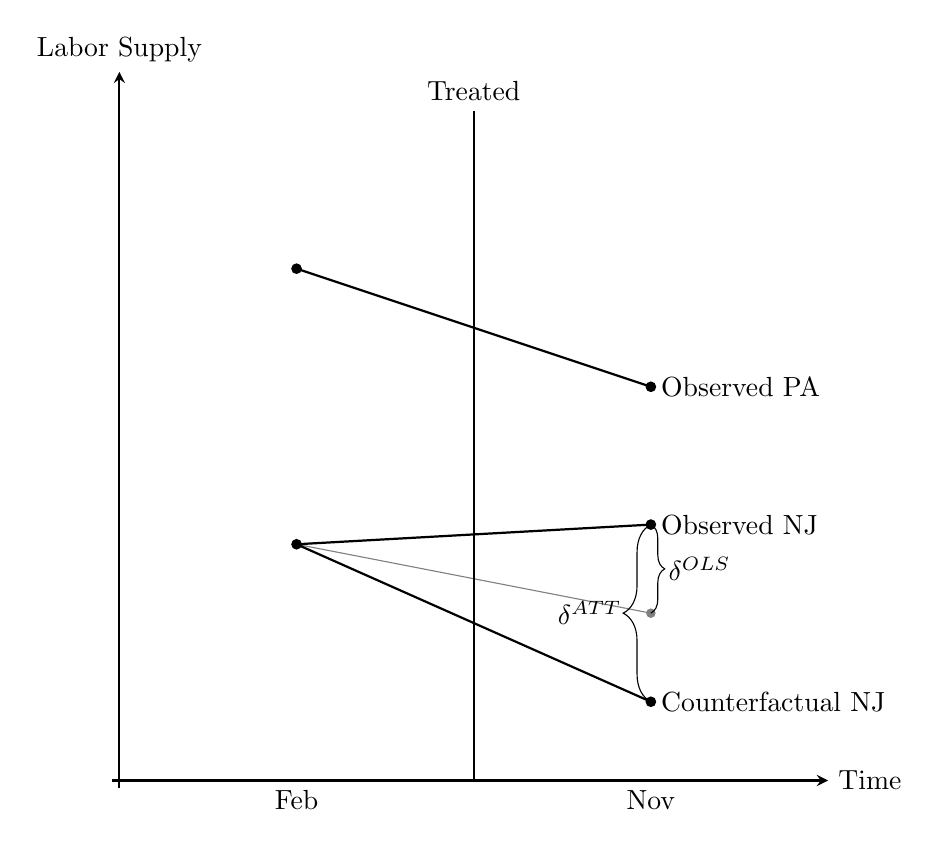
\begin{tikzpicture}
	\draw [thick, -{stealth}] (-.1,0) -- (9,0) node [anchor=west] {Time};
	\draw [thick, -{stealth}] (0,-.1) -- (0,9) node [anchor=south] {Labor Supply};

	\node [anchor=north] at (2.25,0) {Feb};
	\node [anchor=north] at (6.75,0) {Nov};
	
	\draw [thick] (4.5,0) -- (4.5,8.5) node [anchor=south] {Treated};
	\draw [thick] (2.25,6.5) -- (6.75,5) node [anchor=west] {Observed PA}%
		node [pos=0,circle, fill=black, draw=black, inner sep=0pt, minimum width=3pt] {} %
		node [pos=1,circle, fill=black, draw=black, inner sep=0pt, minimum width=3pt] {}; %;
	
	\draw [thick, black] (2.25,3) -- (6.75,3.25) %
		node [pos=0,circle, fill=black, draw=black, inner sep=0pt, minimum width=3pt] {} %
		node [pos=1,circle, fill=black, draw=black, inner sep=0pt, minimum width=3pt] {} %
		coordinate (a1) node [anchor=west, text=black] {Observed NJ};
	\draw [thick, black] (2.25,3) -- (6.75,1) coordinate (a2) %
		node [anchor=west, text=black] {Counterfactual NJ}
		node [pos=1,circle, fill=black, draw=black, inner sep=0pt, minimum width=3pt] {}; %
	
	\draw [black,decorate,decoration={brace,amplitude=10pt,mirror},yshift=0pt] (a1)%
		-- (a2) %
		node (a3) [coordinate, midway] {}%
		node [midway,anchor=east,xshift=-.25cm] {$\delta^{ATT}$};
	
	\begin{pgfonlayer}{bg}
		\draw [thin, gray] (2.25,3) -- (a3) node (a4) [coordinate] {} node [circle, fill=gray, draw=gray, inner sep=0pt, minimum width=3pt] {};
	\end{pgfonlayer}
	\begin{pgfonlayer}{back}
		\draw [decorate,decoration={brace,amplitude=5pt},yshift=0pt] (a1) -- (a4) node [midway,anchor=west,xshift=.1cm] {$\delta^{OLS}$};
	\end{pgfonlayer}
\end{tikzpicture}
	\caption{DD regression diagram without parallel trends}
\end{figure}

\end{frame}


\begin{frame}[plain]
	\begin{center}
	\textbf{Compositional differences violate parallel trends}
	\end{center}
	
	\begin{itemize}
	\item One of the risks of a repeated cross-section is that the composition of the sample may have changed between the pre and post period
	\item Hong (2011) uses repeated cross-sectional data from the Consumer Expenditure Survey (CEX) containing music expenditure and internet use for a random sample of households
	\item Study exploits the emergence of Napter (first file sharing software widely used by Internet users) in June 1999 as a natural experiment
	\item Study compares internet users and internet non-users before and after emergence of Napster
	\end{itemize}

\end{frame}

\begin{frame}[plain]
	\begin{figure}
	\includegraphics{./lecture_includes/Hong_1.pdf}
	\end{figure}
	
\end{frame}

\begin{frame}[shrink=20,plain]
	\begin{figure}
	\includegraphics{./lecture_includes/Hong_2.pdf}
	\end{figure}
	
	Diffusion of the Internet changes samples (e.g., younger music fans are early adopters)
	
\end{frame}



\subsection{Event study}

\begin{frame}
\begin{center}
\textbf{Parallel leads, not trends}
\end{center}

\begin{itemize}

	\item The identifying assumption for all DD designs is some representation of a counterfactual parallel trend
	\item Parallel trends cannot be directly verified because technically one of the parallel trends is an unobserved counterfactual
	\item But one often will check using pre-treatment data to show that the trends had been the same prior to treatment
	\item But, even if pre-trends are the same one still has to worry about other policies changing at the same time (omitted variable bias)

\end{itemize}

\end{frame}

\begin{frame}[plain]
\begin{center}
\textbf{Plot the raw data when there's only two groups}
\end{center}

	\begin{figure}
	\includegraphics[scale=2.5]{./lecture_includes/waldinger_dd_6.pdf}
	\end{figure}

\end{frame}


\begin{frame}[plain]
\begin{center}
\textbf{Differential timing makes pre-treatment undefined for untreated groups}
\end{center}

\begin{itemize}
\item New Jersey treated in late 1992, New York in late 1993, Pennsylvania never treated
\item Pre-treatment:
	\begin{itemize}
	\item New Jersey: $<$1992
	\item New York: $<$1993
	\item Pennsylvania: undefined
	\end{itemize}
\item So how do we check parallel leads?

\end{itemize}

\end{frame}

\begin{frame}[plain]
\begin{center}
\textbf{Randomize treatment dates to control units}
\end{center}

	\begin{figure}
	\includegraphics[scale=0.25]{./lecture_includes/mml_eventstudy}
	\caption{Anderson, et al. (2013) display of raw traffic fatality rates for re-centered treatment states and control states with randomized treatment dates}
	\end{figure}

\end{frame}

\begin{frame}[plain]
\begin{center}
\textbf{Randomized control counties to receive arbitrary dates as treatment can be misleading}
\end{center}

	\begin{figure}
	\includegraphics[scale=0.5]{./lecture_includes/dd.pdf}
	\caption{From one of my studies. Looks decent right?}
	\end{figure}

\end{frame}



\begin{frame}[plain]
	\begin{center}
	\textbf{Event study regression}
	\end{center}
	
	\begin{itemize}
	\item Including leads into the DD model is an easy way to analyze pre-treatment trends
	\item Lags can be included to analyze whether the treatment effect changes over time after assignment
	\item The estimated regression would be:$$Y_{its} = \gamma_s + \lambda_t + \sum_{\tau=-1}^{-q}\gamma_{\tau}D_{s\tau} + \sum_{\tau=0}^m\delta_{\tau}D_{s\tau}+x_{ist}+\varepsilon_{ist}$$
		\begin{itemize}
		\item Treatment occurs in year 0
		\item Includes $q$ leads or anticipatory effects
		\item Includes $m$ leads or post treatment effects
		\end{itemize}
	\end{itemize}
\end{frame}



\begin{frame}[plain]
	\begin{figure}
	\includegraphics[scale=0.5]{./lecture_includes/br1544.pdf}
	\end{figure}
	
Same data as a couple slides ago, leads don't look good
	
\end{frame}


\begin{frame}[plain]
\begin{center}
\textbf{Medicaid and Affordable Care Act example}
\end{center}

\begin{itemize}
\item Miller, et al. (2019) examine a rollout of Medicaid under the Affordable Care Act
\item They link large-scale survey data with administrative death records
\item 9.3 reduction in annual mortality caused by Medicaid expansion
\item Driven by a reduction in disease-related deaths which grows over time
\end{itemize}

\end{frame}

\begin{frame}[plain]

	\begin{figure}
	\includegraphics[scale=0.5]{./lecture_includes/Miller_Medicaid1}
	\end{figure}

\end{frame}

\begin{frame}[plain]

	\begin{figure}
	\includegraphics[scale=0.5]{./lecture_includes/Miller_Medicaid2}
	\end{figure}

\end{frame}

\begin{frame}[plain]

	\begin{figure}
	\includegraphics[scale=0.5]{./lecture_includes/Miller_Medicaid3}
	\end{figure}

\end{frame}


\begin{frame}[plain]

	\begin{figure}
	\includegraphics[scale=0.3]{./lecture_includes/Miller_Medicaid4}
	\caption{Miller, et al. (2019) estimates of Medicaid expansion's effects on on annual mortality}
	\end{figure}

\end{frame}

\begin{frame}[plain]
	\begin{center}
	\textbf{Standard errors in DD strategies}
	\end{center}
	
	\begin{itemize}
	\item Many paper using DD strategies use data from many years -- not just 1 pre and 1 post period
	\item The variables of interest in many of these setups only vary at a group level (say a state level) and outcome variables are often serially correlated
	\item As Bertrand, Duflo and Mullainathan (2004) point out, conventional standard errors often severely understate the standard deviation of the estimators -- standard errors are biased downward (i.e., too small, over reject)
	\end{itemize}
\end{frame}


\begin{frame}[plain]
	\begin{center}
	\textbf{Standard errors in DD -- practical solutions}
	\end{center}
	
	\begin{itemize}
	\item Bertrand, Duflo and Mullainathan propose the following solutions:
		\begin{enumerate}
		\item Block bootstrapping standard errors (if you analyze states the block should be the states and you would sample whole states with replacement for bootstrapping)
		\item Clustering standard errors at the group level (in Stata one would simply add \texttt{, cluster(state)} to the regression equation if one analyzes state level variation)
		\item Aggregating the data into one pre and one post period. Literally works if there is only one treatment data.  With staggered treatment dates one should adopt the following procedure:
			\begin{itemize}
			\item Regress $Y_{st}$ onto state FE, year FE and relevant covariates
			\item Obtain residuals from the treatment states only and divide them into 2 groups: pre and post treatment
			\item Then regress the two groups of residuals onto a post dummy
			\end{itemize}
		\end{enumerate}
	\end{itemize}
\end{frame}

\begin{frame}[plain]

\begin{center}
\textbf{Note about groups}
\end{center}

\begin{itemize}
	\item Correct treatment of standard errors sometimes makes the number of groups very small: in the Card and Krueger study the number of groups is only 2.

\end{itemize}

\end{frame}
	

\begin{frame}[plain]
	\begin{center}
	\textbf{DD Robustness}
	\end{center}
	
	\begin{itemize}
	\item Very common for readers and others to request a variety of ``robustness checks'' from a DD design
	\item Think of these as along the same lines as the leads and lags we already discussed
		\begin{itemize}
		\item Event study (already discussed)
		\item Falsification test using data for alternative control group
		\item Falsification test using alternative ``placebo'' outcome that should not be affected by the treatment
		\end{itemize}
	\end{itemize}
\end{frame}


\begin{frame}[plain]
\begin{center}
\textbf{Within group controls - triple diff}
\end{center}

\begin{table}\centering
		\caption{Differences-in-differences-in-differences}
		\tiny
		\begin{center}
		\begin{tabular}{lll|l|lll}
		\hline \hline
		\multicolumn{1}{l}{\textbf{States}}&
		\multicolumn{1}{c}{\textbf{Group}}&
		\multicolumn{1}{c}{\textbf{Period}}&
		\multicolumn{1}{c}{\textbf{Outcomes}}&
		\multicolumn{1}{c}{$D_1$}&
		\multicolumn{1}{c}{$D_2$}&
		\multicolumn{1}{c}{$D_3$}\\
		\hline
		&&After	&$NJ+T+NJ_t+l_t+D$					\\
	&Low wage employment			&&&$T+NJ_t+l_t+D$			\\
		&&Before	&$NJ$					\\
NJ					&&&&&$D+l_t-s_t$			\\
		&&After	&$NJ+T+NJ_t+s_t$					\\
	&High wage employment		&&	&$T+NJ_t+s_t$				\\
		&&Before	&$NJ$					\\
								\\
&&&&&&$D$
\\
		&&After	&$PA+T+PA_t+l_t$				\\
	&Low wage employment			&&&$T+PA_t+l_t$ \\				
		&&Before	&$PA$					\\
PA					&&&&&$l_t-s_t$		\\
		&&After	&$PA+T+PA_t+s_t$					\\
	&High wage employment		&&&	$T+PA_t+s_t$				\\
		&&Before	&$PA$					\\
		\hline \hline
		\end{tabular}
		\end{center}
	\end{table}

\end{frame}

\begin{frame}[plain]
	\begin{center}
	\textbf{DDD Example by Gruber}
	\end{center}
	
	\begin{figure}
	\includegraphics{./lecture_includes/gruber_ddd_3.pdf}
	\end{figure}
	
\end{frame}

\begin{frame}[plain]
	\begin{center}
	\textbf{DDD in Regression}
	\end{center}
	
	\begin{eqnarray*}
	Y_{ijt} &=& \alpha + \beta_1 X_{ijt} + \beta_2 \tau_t + \beta_3 \delta_j  + \beta_4 D_i + \beta_5(\delta \times \tau)_{jt} \\
	&& +\ \beta_6(\tau \times D)_{ti} +  \beta_7(\delta \times D)_{ij} +  \textcolor{red}{\beta_8(\delta \times \tau \times  D)_{ijt}}+  \varepsilon_{ijt}
	\end{eqnarray*}
	
	\begin{itemize}
	\item The DDD estimate is the difference between the DD of interest and a placebo DD (which is supposed to be zero)
	\item If the placebo DD is non-zero, it might be difficult to convince the reviewer that the DDD removed all the bias 
	\item If the placebo DD is zero, then DD and DDD give the same results but DD is preferable because standard errors are smaller for DD than DDD
	\item But now you have multiple parallel trends assumption - both the control group trends are good counterfactuals, and within-state placebo trends for within-state treatment unit counterfactual trends
	\end{itemize}
	
\end{frame}

\begin{frame}[plain]
\begin{center}
\textbf{Implementing DDD}
\end{center}

	\begin{itemize}
	\item Have to get the structure of the data correct because now you have (1) before and after, (2) treatment and control states, and (3) within state placebo
	\item I give an example in my Mixtape (p. 278) looking at abortion legalization's effect on longterm risky sexual behavior, including do file
	\item Let's review first the paper, then work through the exercise itself using data.
	\end{itemize}
	
\end{frame}

\begin{frame}[plain]


\begin{figure}
	\includegraphics[scale=0.15]{./lecture_includes/aler.png}
	\caption{Longrun effects of abortion legalization on Risky Sex}
	\end{figure}

\end{frame}


\begin{frame}[plain]
\begin{center}
\textbf{Motivation}
\end{center}

\begin{itemize}
	\item Legalization caused teen childbearing to fall by 12\% (Levine 2004)
	\item Gruber, et al. (1999) showed that the marginal child would have been 60\% more likely to live in a single-parent household, 50\% more likely to live in poverty, and 45\% more likely to be a recipient of public services
	\item Mechanism was believed to be non-random selection associated with high risk conditions
\end{itemize}

\end{frame}


\begin{frame}[plain]
\begin{center}
\textbf{Emerging influence}
\end{center}

\begin{itemize}
	\item Donohue and Levitt (2001) linked abortion legalization to declining crime in the 1990s, one of several reasons given for his John Bates Clark award
	\item Freakonomics popularizes the sensational theory
	\item Other papers followed like Charles and Stephens (2006) who find that children exposed \emph{in utero} to legalization were less likely to use illegal substances

\end{itemize}

\end{frame}

\begin{frame}[plain]
\begin{center}
\textbf{Controversy}
\end{center}

\begin{itemize}
	\item Triple diff by Joyce finds no evidence for it when using an (arbitrary) cutoff of the median abortion rate within early repeal treatment states
	\item Foote and Goetz (2008) argue the abortion ratio was constructed incorrectly, and report a coding error leaving out state-year fixed effects; construction problem destroys results, state-year fixed effects somewhat attenuates
	\item Literature stops and theory is ignored
\end{itemize}

\end{frame}

\begin{frame}[plain]
\begin{center}
\textbf{In defense of Steve Levitt}
\end{center}

		\begin{itemize}
		\item I want to remind people though: we only know about the coding error bc Levitt posted his do files and gave them to anyone who asked (very easy to ``lose do files'')
		\item Levitt had and has oodles of scientific integrity for his willingness to cooperate; not always the case
		\end{itemize}

\end{frame}

\begin{frame}[plain]

\begin{quote}
``If abortion lowers homicide rates by 20 -- 30\%, then it is likely to have affected an
entire spectrum of outcomes associated with well-being: infant health, child development,
schooling, earnings and marital status. Similarly, the policy implications are
broader than abortion. Other interventions that affect fertility control and that lead
to fewer unwanted births -- contraception or sexual abstinence -- have huge potential
payoffs. In short, a causal relationship between legalized abortion and crime has
such significant ramifications for social policy and at the same time is so controversial,
that further assessment of the identifying assumptions and their robustness to
alternative strategies is warranted.'' Ted Joyce in his triple diff paper \end{quote}

\end{frame}


\begin{frame}[plain]

\begin{figure}[htb]
\centering
\includegraphics[scale=0.04]{./lecture_includes/scotteinstein.jpg}
\caption{Light bending around the sun, predicted by Einstein, and confirmed in a natural experiment involving an eclipse. Artwork by Seth Hahne \textcopyright.}
\end{figure}

\end{frame}

\begin{frame}[plain]
\begin{center}
\textbf{In defense of falsifiable predictions}
\end{center}

\begin{itemize}
\item Theories which make falsifiable predictions (comparative statics) are \emph{more} convincing of causal effects than simpler reduced form studies
\item Great paper by Coleman on (2019) Snow's rhetoric in his 1849 essay and his 1855 book on cholera -- mounts different data to make his argument, some of which is of this nature
\item Those predictions are threefold:
	\begin{itemize}
	\item Where we should find effects
	\item Where we should not find effects
	\item The kind of effects we should find
	\end{itemize}
\item If all three are met, an identified causal effect becomes epistemologically more credible
\end{itemize}

\end{frame}


\begin{frame}[plain]

\begin{center}
\textbf{Falsifiable predictions contained in a diff-in-diff}
\end{center}

\begin{figure}
	\includegraphics[scale=0.25]{./lecture_includes/cohort_id.jpg}
	\caption{Group-time differential exposure predicts a temporary parabolic ATT}
	\end{figure}

\end{frame}

\begin{frame}[plain]

	\begin{figure}
	\includegraphics[scale=0.6]{./lecture_includes/bf15_dd-.png}
	\caption{Raw data for repeal and Roe states.}
	\end{figure}

\end{frame}




\begin{frame}[plain]
\begin{center}
\textbf{Estimating equation}
\end{center}

\begin{eqnarray*}
Y_{st} &=& \beta_1Repeals +\beta_2 DTt +\beta_{3t} Repeal_s \times DT_t +X_{st} \psi+\alpha_{s}DS_s \\
&+&  \gamma_1t + \gamma_{2s} \times t + \varepsilon_{st}
\end{eqnarray*}

\end{frame}

\begin{frame}[plain]

\begin{figure}
	\includegraphics[scale=0.75]{./lecture_includes/bf15_dd.pdf}
	\caption{Differences in black female gonorrhea incidence between repeal and \emph{Roe} cohorts.}
	\end{figure}

\end{frame}

\begin{frame}[plain]
\begin{center}
\textbf{Assuaging doubt}
\end{center}

\begin{itemize}

\item Maybe spurious - something happened in those years, but what?
\item Crack epidemic maybe? But we control for the crack index by Fryer, et al.
\item Maybe something else - let's try a within-state control group (the older cohort)

\end{itemize}

\end{frame}


\begin{frame}[plain]
\begin{center}
\textbf{DDD Equation}
\end{center}

\begin{eqnarray*}
	Y_{ast} &=& \beta_1\,Repeal_s + \beta_2DT_t +\beta_3\,DA+ \beta_{4t}\,Repeal_s\cdot DT_t   +  \nonumber \\
	        &+& \beta_5\,Repeal_s\cdot DA + \beta_{6t}\,DA\cdot DT_t + \textcolor{red}{\beta_{7t}\,Repeal_s\cdot DA \cdot DT_t}  \nonumber \\
                 &+& X_{st}\xi + \alpha_{1s}DS_s + \alpha_{2s}DS_s\cdot DA + \gamma_1\,t + \gamma_{2s}DS_s\cdot t + \gamma_3DA\cdot t \nonumber \\
                 &+&  \gamma_{4s}DS_s\cdot DA \cdot t + \epsilon_{ast}
\end{eqnarray*}

One will be dropped, but I want to focus your attention on the number of interactions needed to identify DDD parameters

\end{frame}



\begin{frame}[plain]
\begin{center}
\textbf{Stacking Structure}
\end{center}

\begin{figure}
	\includegraphics[scale=0.5]{./lecture_includes/abortion_structure}
	\caption{DDD data structure is complicated}
	\end{figure}

\end{frame}

\begin{frame}[plain]
\begin{center}
\textbf{DDD Results}
\end{center}

	\begin{figure}
	\includegraphics[scale=0.75]{./lecture_includes/bf15_ddd.pdf}
	\end{figure}

\end{frame}

\begin{frame}[plain]
\begin{center}
\textbf{My original conclusions}
\end{center}

\begin{itemize}
\item Model made narrow predictions of a \emph{parabola} within a given window but only for the treatment cohort
\item Amazingly we actually found that very shape in the DD -- did we vindicate Gruber, et al. and Donohue and Levitt then?
\item Also used older group as within-state controls in a DDD, and still found the parabola, though not as great a look as DD which is a bit of a red flag
\item Paper also illustrates the usefulness of having a specific theoretical prediction. Limits the number of competing hypotheses (Popperian type of reasoning). 
\item But was I done? Look back at the table
\end{itemize}

\end{frame}

\begin{frame}[plain]
\begin{center}
\textbf{Going beyond Cornwell and Cunningham (2013)}
\end{center}

	\begin{figure}
	\includegraphics[scale=0.2]{./lecture_includes/cohort_id2}
	\caption{Second theoretical prediction - this time for 20-24 year olds}
	\end{figure}

\end{frame}

\begin{frame}[plain]

	\begin{figure}
	\includegraphics[scale=0.7]{./lecture_includes/bf20_dd.pdf}
	\end{figure}

\end{frame}


\begin{frame}[plain]
\begin{center}
\textbf{Second prediction fails second DD model}
\end{center}


\begin{itemize}

\item Ugh.  \emph{lo tov} (Hebrew to English: not good)
\item Well, maybe DDD will look better?

\end{itemize}

\end{frame}


\begin{frame}[plain]

	\begin{figure}
	\includegraphics[scale=0.7]{./lecture_includes/bf20_ddd.pdf}
	\end{figure}

\end{frame}

\begin{frame}[plain]
\begin{center}
\textbf{Second predictions fails DDD too}
\end{center}

\begin{itemize}
\item Notice that when we exploited just one testable prediction, we found evidence
\item But when we exploit all of the testable predictions, the results fall apart, suggesting original DD was spurious 
\item Imagine for a moment, though -- what if we had seen the group-time ATT moving with the cohort as they aged?
\item Other alternative is the repeal-Roe effects dissipate by early to late 20s, but what does Ockham's Razor say is the more credible explanation?
\item Perhaps the Gruber, et al. (1999) and Donohue and Levitt (2001) hypothesis was always spurious
\end{itemize}

\end{frame}

\begin{frame}[plain]
\begin{center}
\textbf{Stata replication}
\end{center}

Let's replicate this using the abortion.do file. Pay close attention to the stacking of the data by group-state, not just state, and the exact way in which the interactions must therefore be constructed

\end{frame}


\begin{frame}[plain]
	\begin{center}
	\textbf{Falsification test with alternative outcome}
	\end{center}
	
	\begin{itemize}
	\item The within-group control group (DDD) is a form of placebo analysis using the same \emph{outcome}
	\item But there are also placebos using a \emph{different} outcome -- but you need a hypothesis of mechanisms to figure out what is in fact a \emph{different outcome}
	\item Figure out what those are, and test them -- finding no effect raises the epistemological credibility of the first result, interestingly
	\item Cheng and Hoekstra (2013) examine the effect of castle doctrine gun laws on non-gun related offenses like grand theft auto and find no evidence of an effect
	\end{itemize}
\end{frame}



\begin{frame}[plain]
\begin{center}
\textbf{Rational addiction as a placebo critique}
\end{center}


Sometimes, an empirical literature may be criticized using nothing more than placebo analysis

\begin{quote}``A majority of [our] respondents believe the literature is a success story that demonstrates the power of economic reasoning.  At the same time, they also believe the empirical evidence is weak, and they disagree both on the type of evidence that would validate the theory and the policy implications. Taken together, this points to an interesting gap.  On the one hand, most of the respondents claim that the theory has valuable real world implications.  On the other hand, they do not believe the theory has received empirical support.''
\end{quote}

\end{frame}

\begin{frame}[plain]
\begin{center}
\textbf{Placebo as critique of empirical rational addiction}
\end{center}

\begin{itemize}
	\item Auld and Grootendorst (2004) estimated standard ``rational addiction'' models (Becker and Murphy 1988) on data with milk, eggs, oranges and apples.  
	\item They find these plausibly non-addictive goods are addictive, which casts doubt on the empirical rational addiction models.
\end{itemize}

\end{frame}

\begin{frame}[plain]
\begin{center}
\textbf{Placebo as critique of peer effects}
\end{center}

\begin{itemize}
	\item Several studies found evidence for ``peer effects'' involving inter-peer transmission of smoking, alcohol use and happiness tendencies
	\item Christakis and Fowler (2007) found significant network effects on outcomes like obesity
	\item Cohen-Cole and Fletcher (2008) use similar models and data and find similar network ``effects'' for things that \emph{aren't} contagious like acne, height and headaches
	\item Ockham's razor - given social interaction endogeneity (Manski 1993), homophily more likely explanation
\end{itemize}

\end{frame}





\subsection{Differential timing}

\begin{frame}
\begin{figure}
\includegraphics[scale=0.25]{./lecture_includes/federalism_sticker.png}
\end{figure}

\end{frame}

\begin{frame}[plain]
\begin{center}
\textbf{State federalism and differential timing}
\end{center}

\begin{itemize}
\item We've been considering situations where treatment occurs in one area for the most part
\item But the modal situation is when there is \emph{differential timing}
\item This happens in America usually because each area (state, municipality) will adopt a policy whenever they want to, which creates tendencies for roll out to occur
\item Example might be the minimum wage though we will look at others
\end{itemize}

\end{frame}



\begin{frame}[plain]
	\begin{figure}
	\includegraphics[scale=0.5]{./lecture_includes/cheng_and_hoekstra_jhr.png}
	\end{figure}

\end{frame}


\begin{frame}[plain]
	\begin{center}
	\textbf{Summary}
	\end{center}
	
	\begin{itemize}
	\item Cheng and Hoekstra (2013) are interested in whether expansions to ``castle doctrine statutes'' at the state level increase or decrease gun violence.  
	\item Prior to these expansions, English common law principle required ``duty to retreat'' before using lethal force against an assailant except when the assailant is an intruder in the home
		\begin{itemize}
		\item The home is one's ``castle'' -- hence, ``castle doctrine''
		\item When intruders threatened the victim in the home, the duty to retreat was waived and lethal force in self-defense was allowed
		\end{itemize}
	\end{itemize}
\end{frame}

\begin{frame}[plain]
	\begin{center}
	\textbf{Castle doctrine law explained}
	\end{center}
	
	\begin{itemize}
	\item In 2005, Florida passed a law that expanded self-defense protections beyond the house
		\begin{itemize}
		\item 2000 to 2010, 21 states explicitly put ``castle doctrine'' into statute, and (more importantly) extended it to places outside the home
		\item In other words, 21 states removed the duty to retreat in specified circumstances
		\end{itemize}
	\item Other changes:
		\begin{itemize}
		\item Presumption of reasonable fear is added
		\item Civil liability for those acting under the law is removed
		\end{itemize}
	\end{itemize}
\end{frame}

\begin{frame}[plain]
	\begin{center}
	\textbf{Economic theory predicts more lethal homicides}
	\end{center}
	
	\begin{itemize}
	\item Workers supply legal or illegal labor and are therefore responsive to costs and benefits
	\item Castle doctrine expansions lowered the (expected) cost of killing someone in self-defense
	\item If people are rational, then lowering the price of lethal self-defense should increase lethal homicides
	\end{itemize}
\end{frame}

\begin{frame}[plain]
	\begin{center}
	\textbf{Economic theory also predicts less crime from deterrence}
	\end{center}
	
	\begin{itemize}
		\item Although deterrence is a theoretical possibility, note that the goal of the laws was to protect enhance victim rights, not deter crime
		\item Testable prediction with data and same design
	\end{itemize}
\end{frame}



\begin{frame}[plain]
	\begin{center}
	\textbf{Treatment passage}
	\end{center}
	
	\begin{itemize}
	\item Summary:
		\begin{itemize}
		\item 21 states passed laws removing ``duty to retreat'' in places outside the home
		\item 17 states removed ``duty to retreat'' in any place one had a legal right to be
		\item 13 states include a presumption of reasonable fear
		\item 18 states remove civil liability when force was justified under law
		\end{itemize}
	\end{itemize}
\end{frame}

\begin{frame}[plain]
	\begin{center}
	\textbf{Cheng and Hoekstra's identification strategy}
	\end{center}
	
	\begin{itemize}
	\item Panel fixed effects estimation$$Y_{it} = \beta_1 D_i + \beta_2 T_t + \beta_3 (CDL_{it}) + \alpha_1X_{it} + c_i + u_t + \varepsilon_{it}$$
	\item $CDL$ is a fraction between 0 and 1 depending on the percent of the year the state has a castle doctrine law 
	\item Preferred specifications includes ``region-by-year fixed effects'' 
	\end{itemize}
\end{frame}


\begin{frame}[plain]
	\begin{center}
	\textbf{Data}
	\end{center}
	
	\begin{itemize}
	\item FBI Uniform Crime Reports Part 1 Offenses (2000-2010)
		\begin{itemize}
		\item State-level crime rates, or ``offenses per 100,000 population''
		\item Falsification outcomes: motor vehicle theft and larceny
		\end{itemize}
	\item Dataset on justifiable homicides by private citizens
	\end{itemize}
\end{frame}


\begin{frame}[plain]
\begin{center}
\textbf{Outcomes (in order)}
\end{center}

\begin{itemize}
	\item Deterrence and homicide outcomes:
		\begin{enumerate}
		\item Burglary: the unlawful entry of a structure to commit a felony or a theft
		\item Robbery: the talking or attempting to take anything of value from the care, custody or control of a person or persons by force or threat of force or violence and/or putting the victim in fear
		\item Aggravated assault: unlawful attack by one person upon another for the purpose of inflicting severe or aggravated bodily injury
		\end{enumerate}
	\item Homicide categories
		\begin{enumerate}
		\item Total homicides -- murder plus non-negligent manslaughter ($\sim$14,000 per year)
		\item  Justifiable homicides by private citizens ($\sim$250/year)
		\end{enumerate}
\end{itemize}

\end{frame}

\begin{frame}[plain]
	\begin{center}
	\textbf{Inference: Clustering}
	\end{center}
	
	\begin{itemize}
	\item Statistical inference: cluster standard errors at the state level
		\begin{itemize}
		\item Are disturbances random draws from individually identical distribution? 
		\item It's likely that within a state, unobserved determinants of crime are serially correlated
		\item They follow Bertand, Duflo and Mullainathan (2004) and adjust for serial correlation in unobserved disturbances within states at the level of the treatment 
		\end{itemize}
	\end{itemize}
\end{frame}

\begin{frame}[plain]
\begin{center}
\textbf{Inference: Fisher's sharp null}
\end{center}

		\begin{itemize}
		\item How likely is it that we estimate effects of this magnitude when using randomly chosen pre-treatment time periods and randomly assigning placebo treatments?
		\item Randomizes dates within-state for the pre-treatment period ($<$2000)
		\item Randomization inference and exact p-values
		\end{itemize}

\end{frame}


\begin{frame}[plain]
	\begin{center}
	\textbf{Region-by-year fixed effects}
	\end{center}
	
	\begin{itemize}
	\item Absent passing castle doctrine laws, outcomes in these 21 states would have changed similar to other states in their same region
		\begin{itemize}
		\item Recall the ``region-by-year fixed effects'' in the $X$ term
		\item By including ``region-by-year fixed effects'', they are arguing that unobserved changes in crime are running ``parallel'' to the treatment states within region over time
		\item Need not hold across regions since the across region variation is not being used in this analysis due to the saturation of the model with ``region-by-year fixed effects''
		\end{itemize}
	\end{itemize}
\end{frame}



\begin{frame}[plain]
\begin{center}
\textbf{State specific time trends}
\end{center}

		\begin{itemize}
		\item Alabama, et al. dummy interacted with TREND which equals 1 in 2000, 2 in 2001, \dots , 11 in 2010
		\item Forces the identification to come from variation in outcomes around the state-specific linear trend 
			\begin{itemize}
			\item Outcomes must be large enough and different enough from a state-specific linear trend otherwise it is collinear with the state-trend
			\item Same argument applies to any control though
			\item Goodman-Bacon (2019) suggests group-trends are less taxing and satisfying than unit-specific trends
			\end{itemize}
		\end{itemize}

\end{frame}

\begin{frame}[plain]
	\begin{center}
	\textbf{Control variables}
	\end{center}
	
	\begin{itemize}
	\item Controls (X matrix in earlier equation)
		\begin{itemize}
		\item Full-time police employment per 100,000 state residents from the LEKOA data (FBI data)
		\item Persons incarcerated in state prison per 100,000 residents
		\item Shares of white/black men in 15-24 and 25-44 age groups
		\item State per capita spending on public assistance
		\item State per capita spending on public welfare
		\end{itemize}
	\end{itemize}
\end{frame}

\begin{frame}[plain]
	\begin{center}
	\textbf{Parallel Leads}
	\end{center}
	
	\begin{itemize}
	\item Look at each set of treatment states against never-treated figure by figure (rare)
	\item Use a one-period lead in the regression model (not as common)
	\item I'm going to look at event study coefficients (most common)
	\end{itemize}
\end{frame}




\begin{frame}[plain]
	\begin{center}
	\textbf{Step one: Falsification test}
	\end{center}
	
	\begin{itemize}
	\item Policy-makers are not just randomly flipping coins when passing laws, but presumably do so because of things they observe on the ground 
	\item Address concerns up front this isn't driven by spurious crime results
	\item Cheng and Hoekstra (2013) present falsification of larceny and motor vehicle theft first, then results
	\end{itemize}
\end{frame}

\begin{frame}[plain]
\begin{center}
\textbf{Step one (cont.)}
\end{center}

\begin{itemize}
	\item Results will be presented separately under six different specifications
		\begin{itemize}
		\item Each new specification adds more controls
		\end{itemize}
	\item Pop quiz: What should you expect to find on key variables of interest when conducting a falsification and why?
\end{itemize}

\end{frame}

\begin{frame}[plain]
\begin{center}
\textbf{Answer}
\end{center}

		\begin{itemize}
		\item No statistically significant association between the CDL passage and the placebos; preferably precise zeroes
		\item No association on the one-year lead either
		\item Basically, you should not find effects where there are no theoretical policy effects; gun laws shouldn't affect non-violent offenses
		\end{itemize}
\end{frame}


\begin{frame}[plain]
\begin{center}
\textbf{Step one (cont.)}
\end{center}

\begin{itemize}
	\item How do you interpret coefficients?
		\begin{itemize} 
		\item His model is ``log outcomes'' regressed onto a dummy variable (level), so these are semi-elasticities and approximate percentage changes -- but you should transform them by taking the exponential of each coefficient and then differencing it from one to find the actual percentage change
		\item Ex: CDL = -0.0137 (column 12, Table 3, ``Log (larceny rate)'' outcome.)  Exp(-0.0137) = 0.986, and so 1-0.986 = 1.4.  Thus, CDL reduced larceny rates by 1.4 percent, which is not statistically significant.  
		\end{itemize}
\end{itemize}

\end{frame}

\begin{frame}[plain]
	\begin{center}
	\textbf{Results -- Falsification Exercise}
	\end{center}
	
	\begin{figure}
	\includegraphics[scale=0.4]{./lecture_includes/cheng3.pdf}
	\end{figure}
\end{frame}

\begin{frame}[plain]
	\begin{center}
	\textbf{Step two: testing the deterrence hypothesis}
	\end{center}
	
	\begin{itemize}
	\item Having found no effect on their placebos, Cheng and Hoekstra (2013) examine the effect of CDL on three deterrence outcomes: burglary, robbery and aggravated assault
		\begin{itemize}
		\item They will, again, have six specifications per outcome in the ``weighted'' regression, and then another five for the ``unweighted'' regression
		\end{itemize}
	\item Pop quiz: What does deterrence look like?
	\end{itemize}
\end{frame}

\begin{frame}[plain]
\begin{center}
\textbf{Answer}
\end{center}

		\begin{itemize}
		\item Negative signs on the CDL variable is consistent with deterrence -- these crimes were ``deterred'', in other words
		\item Based on early work by Becker (1968) and 1970s work by his student Isaac Ehrlich; higher probabilities of getting hurt in public may cause offenders to avoid violence in public altogether
		\item Bounds on the magnitudes from the standard errors are used to provide some confidence about the estimates as well
		\end{itemize}

\end{frame}

\begin{frame}[plain]
	\begin{center}
	\textbf{Results -- Deterrence}
	\end{center}
	
	\begin{figure}
	\includegraphics[scale=0.4]{./lecture_includes/cheng4.pdf}
	\end{figure}
\end{frame}

\begin{frame}[plain]
	\begin{center}
	\textbf{Conclusion}
	\end{center}
	
	\begin{itemize}
	\item ``In short, these estimates provide strong evidence against the possibility that castle doctrine laws cause economically meaningful deterrence effects'' (p. 17)
		\begin{itemize}
		\item Translation: They can't find evidence of large deterrence effects
		\end{itemize}
	\item ``Thus, while castle doctrine law may well have benefits to those legally justified in protecting themselves in self-defense, there is no evidence that the law provides positive spillovers by deterring crime more generally'' (p. 17)
		\begin{itemize}
		\item They note in footnote 24 that they cannot measure the benefits to victims whose crimes were deterred, or the benefits from lower legal costs; their focus is limited to whether it deterred the crimes, not whether the net benefits from the laws were positive
		\item Obviously, if there is no deterrence, though, then the net benefits are lower from CDL than they would be if they did deter
		\end{itemize}
	\end{itemize}
\end{frame}

\begin{frame}[plain]
	\begin{center}
	\textbf{Step 3: Homicides}
	\end{center}
	
	\begin{itemize}
	\item The key finding in this study focuses on CDL and its effect on homicides and non-negligent manslaughter
	\item Pop quiz: what should the sign on CDL be here?
	\end{itemize}
\end{frame}


\begin{frame}[plain]
\begin{center}
\textbf{Answer}
\end{center}

\begin{itemize}
	\item Effects should be \textbf{positive}
	\item Cheng and Hoekstra want to show the raw data, but have differential timing
	\item Differential timing means you can't show pre-treatment raw data for the never-treated groups
	\item So they show it one by one -- which isn't the most aesthetically pleasing way to do it, but which has the benefit of being transparent
\end{itemize}

\end{frame}

\begin{frame}[plain]
\begin{center}
\textbf{Parallel pre-treatment trends}
\end{center}

\begin{itemize}
	\item Keep your eyes on whether pre-treatment trends are parallel for treatment and control groups
		\begin{itemize}
		\item Remember, though -- he needs parallel trends within-region -- these figures don't show that
		\item But starting with pictures and raw data has value
		\end{itemize}
	\end{itemize}
\end{frame}


\begin{frame}[plain]
	\begin{center}
	\textbf{Log Homicide Rates -- 2005 Adopter = Florida}
	\end{center}
	
	\begin{figure}
	\includegraphics[scale=0.4]{./lecture_includes/cheng5.pdf}
	\end{figure}
\end{frame}


\begin{frame}[plain]
	\begin{center}
	\textbf{Log Homicide Rates -- 2006 Adopter (13 states)}
	\end{center}
	
	\begin{figure}
	\includegraphics[scale=0.4]{./lecture_includes/cheng6.pdf}
	\end{figure}
\end{frame}

\begin{frame}[plain]
	\begin{center}
	\textbf{Log Homicide Rates -- 2007 Adopter (4 states)}
	\end{center}
	
	\begin{figure}
	\includegraphics[scale=0.4]{./lecture_includes/cheng7.pdf}
	\end{figure}
\end{frame}

\begin{frame}[plain]
	\begin{center}
	\textbf{Log Homicide Rates -- 2008 Adopter (2 states)}
	\end{center}
	
	\begin{figure}
	\includegraphics[scale=0.4]{./lecture_includes/cheng8.pdf}
	\end{figure}
\end{frame}


\begin{frame}[plain]
	\begin{center}
	\textbf{Log Homicide Rates -- 2009 Adopter = Montana}
	\end{center}
	
	\begin{figure}
	\includegraphics[scale=0.4]{./lecture_includes/cheng9.pdf}
	\end{figure}
\end{frame}



\begin{frame}[plain]
\begin{center}
\textbf{Modeling}
\end{center}

\begin{itemize}
		\item He uses a class of estimators more appropriate for ``counts'' called ``count models'', like the negative binomial estimated with maximum likelihood
		\item Results are robust to least squares and count models
\end{itemize}

\end{frame}

%\begin{frame}[plain]
%	\begin{center}
%	\textbf{Homicide -- OLS}
%	\end{center}
	
%	\begin{figure}
%	\includegraphics[scale=0.4]{./lecture_includes/cheng11.pdf}
%	\end{figure}
%\end{frame}


\begin{frame}[plain]
	\begin{center}
	\textbf{Homicide -- Negative Binomial; Murder -- OLS}
	\end{center}
	
	\begin{figure}
	\includegraphics[scale=0.4]{./lecture_includes/cheng12.pdf}
	\end{figure}
\end{frame}

\begin{frame}[plain]
	\begin{center}
	\textbf{Fisher sharp null}
	\end{center}
	
Move the 11-year panel back one year at a time (covering 1960-2009) and estimate 40 placebo ``effects'' of passing CDL 1 to 40 years earlier


	\begin{table}
	\begin{tabular}{ccc}
	\hline
	\multicolumn{1}{c}{Method}&
	\multicolumn{1}{c}{Average }&
	\multicolumn{1}{c}{Estimates larger }\\
	\multicolumn{1}{c}{}&
	\multicolumn{1}{c}{estimate}&
	\multicolumn{1}{c}{than actual estimate}\\
	\hline
	Weighted OLS & --0.003 & 0/40\\
	Unweighted OLS & 0.001 & 1/40 \\
	Negative binomial & 0.001 & 0/40 \\
	\hline
	\end{tabular}
	\end{table}

\end{frame}

\begin{frame}[plain]
\begin{center}
\textbf{My replication using event study plots}
\end{center}

	\begin{figure}
	\includegraphics[scale=0.5]{./lecture_includes/event_cheng1.pdf}
	\caption{Homicide event study plots using coefplot}
	\end{figure}

\end{frame}

\begin{frame}[plain]

	\begin{figure}
	\includegraphics[scale=0.5]{./lecture_includes/event_cheng2.pdf}
	\caption{Homicide event study plots using twoway}
	\end{figure}

\end{frame}


\begin{frame}[plain]

	\begin{figure}
	\includegraphics[scale=0.5]{./lecture_includes/event_cheng3.pdf}
	\caption{Homicide event study plots using twoway and force early leads into one coefficient}
	\end{figure}

\end{frame}

\begin{frame}[plain]

	\begin{figure}
	\includegraphics[scale=0.5]{./lecture_includes/event_cheng4.pdf}
	\caption{Homicide event study plots using twoway dropping imbalanced states}
	\end{figure}

\end{frame}

\begin{frame}[plain]
	\begin{center}
	\textbf{Interpretation}
	\end{center}
	
	\begin{itemize}
	\item No evidence that Castle Doctrine/Stand Your Ground Laws deter violent crimes such as burglary, robbery and aggravated assault
	\item These laws do lead to an 8\% net increase in homicide rates, translating to around 600 additional homicides \emph{per year} across the 21 adopting states
	\item Unlikely that all of the additional homicides were legally justified
	\item Incentives matter in some contexts (lethal force) but not others (deterrence)
	\end{itemize}
\end{frame}


\begin{frame}[plain]
\begin{center}
\textbf{Where to from here?}
\end{center}

\begin{itemize}
\item Now that we've reviewed the twoway fixed effects with treatment that differed across time, how does this more general form of ``differential timing'' compare with the 2x2 DD that we reviewed?
\item Complicated derivation, but simple interpretation - twoway fixed effects with differential timing estimates a weighted average of all 2x2
\item Andrew Goodman-Bacon (2018; 2019) and Callaway and Sant'ann (2019)
\item I will be making the argument that under certain \emph{modal} situations, the twoway fixed effects model has major problems, even fatal ones, due to biases even when parallel trends plausibly holds
\end{itemize}

\end{frame}

\begin{frame}[plain]
\begin{figure}
\includegraphics[scale=0.45]{./lecture_includes/nber_bacon_goodman.png}
\end{figure}

\end{frame}


\begin{frame}[plain]
\begin{center}
\textbf{Reminder of 2x2 DD}
\end{center}

To understand differential timing, we need to remind ourselves 2x2 form

\begin{eqnarray*}
\widehat{\delta}^{2x2}_{kU} = \bigg ( \overline{y}_k^{post(k)} - \overline{y}_k^{pre(k)} \bigg ) - \bigg ( \overline{y}_U^{post(k)} - \overline{y}_U^{pre(k)} \bigg )
\end{eqnarray*}
Post to pre difference for treatment group compared to the post to pre difference for \emph{never} treated


\end{frame}


\begin{frame}[plain]
\begin{center}
\textbf{Different treatment dates by panel unit}
\end{center}

\begin{eqnarray*}
y_{it} &=& \underbrace{\beta D_{i} + \tau Post_{t} + \delta (D_i \times Post_t) + X_{it} + \alpha_i + \alpha_t+ \varepsilon_{it}}_{2x2 \text{ }DD} \\
y_{it} &=& \underbrace{ \delta D_{it} + X_{it} + \alpha_i + \alpha_t + \epsilon_{it}}_{Twoway\text{ }FE}
\end{eqnarray*}

 We know a lot about 2x2, but about the twoway fixed effects estimator when it comes to DD designs

\end{frame}



\begin{frame}[plain]
\begin{center}
\textbf{Decomposition Preview}
\end{center}

\begin{itemize}
\item Linear panel models estimate a treatment parameter that is a weighted average over all 2x2 in your sample
\item The estimator is a weighted average of all potential $\delta^{2\times 2}$ in which treated units act as both controls and treatment depending on the situation
\item Weights are function of sample sizes of each ``group'' and the variance of the treatment dummies for the groups
\end{itemize}

\end{frame}

\begin{frame}[plain]
\begin{center}
\textbf{Decomposition (cont.)}
\end{center}

\begin{itemize}
\item Under the assumptions of variance weighted common trends (VWCT) and time invariant treatment effects, the estimator called the variance weighted ATT is a weighted average of all possible ATTs
\item Under more restrictive assumptions it perfectly matches the ATT
\item Time varying treatment effects generate a bias that needs to be accounted for
\end{itemize}

\end{frame}

\begin{frame}[plain]
\begin{center}
\textbf{3 Group Example}
\end{center}

\begin{itemize}
\item Suppose two treatment groups (k,l) and one untreated group (u)
\item k,l define the groups based on when they receive treatment (differently in time) with k receiving it later than l
\item Denote $\overline{D}_k$ as the share of time each group spends in treatment status
\item Denote $\widehat{\delta}_{ab}^{2x2,j}$ as the canonical $2\times 2$ DD estimator for groups a and b where $j$ is the treatment group
\item So what are the possible $2 \times 2$ combinations?
\end{itemize}

\end{frame}


\begin{frame}[plain]
\begin{center}
\textbf{How many 2x2?}
\end{center}

\begin{itemize}
\item A lot!
\item When there's three groups - a never treated (U), an early treated (k) and a late treated (l), there are four 2x2s
\item But typically, we have more than 3 groups making the number of potential 2x2 even larger
\item With $K$ timing groups and one untreated group, there are $K^2$ distinct 2x2 DDs
\end{itemize}

\end{frame}

\begin{frame}[plain]
\begin{center}
\textbf{$K^2$ distinct DDs}
\end{center}

Assume 3 timing groups (a, b and c) and one untreated group (U).  Then there should be 9 2x2 DDs.  Here they are:


\begin{center}
\begin{tabular}{c|c|c}
\multicolumn{1}{l}{} &
\multicolumn{1}{l}{} &
\multicolumn{1}{l}{} \\
\midrule
a to b & b to a & c to a \\
a to c & b to c & c to b \\
a to U & b to U & c to U \\
\midrule
\end{tabular}
\end{center}


\end{frame} 


\begin{frame}[plain]
\begin{center}
\textbf{Simple example with 3 groups}
\end{center}

\begin{itemize}
\item We'll stick with two groups, k and l, who will get the treatment at $t^*_k$ and $t^*_l$, and the third group $U$ will never get treated
\item The earlier period before anyone is treated is ``pre'', the period between k and l treatment is ``mid'', and the period after l is treated is ``post''
\end{itemize}

\end{frame} 

\begin{frame}[plain]

	\begin{figure}
	\includegraphics[scale=0.5]{./lecture_includes/bacon_goodman_2.png}
	\end{figure}

\end{frame}



\begin{frame}[plain]
\begin{center}
\textbf{Three important 2x2 DDs}
\end{center}

\begin{eqnarray*}
\widehat{\delta}^{2x2}_{kU} &=& \bigg ( \overline{y}_k^{post(k)} - \overline{y}_k^{pre(k)} \bigg ) - \bigg ( \overline{y}_U^{post(k)} - \overline{y}_U^{pre(k)} \bigg ) \\
\widehat{\delta}^{2x2}_{kl} &=& \bigg ( \overline{y}_k^{mid(k,l)} - \overline{y}_k^{pre(k)} \bigg ) - \bigg ( \overline{y}_l^{mid(k,l)} - \overline{y}_l^{pre(k)} \bigg ) \\
\widehat{\delta}^{2x2}_{lk} &=& \bigg ( \overline{y}_l^{post(l)} - \overline{y}_l^{mid(k,l)} \bigg ) - \bigg ( \overline{y}_k^{post(l)} - \overline{y}_k^{mid(k,l)} \bigg ) 
\end{eqnarray*}
where the first 2x2 is any timing group compared to untreated, the second is a group compared to yet-to-be-treated timing group, and the last is the eventually-treated compared to the already-treated controls.

\end{frame}


\begin{frame}[plain]
$$\widehat{\delta}^{2x2}_{kU} = \bigg ( \overline{y}_k^{post(k)} - \overline{y}_k^{pre(k)} \bigg ) - \bigg ( \overline{y}_U^{post(k)} - \overline{y}_U^{pre(k)} \bigg ) $$
	\begin{figure}
	\includegraphics[scale=0.5]{./lecture_includes/bacon_goodman_3.png}
	\end{figure}

\end{frame}

\begin{frame}[plain]
$$\widehat{\delta}^{2x2}_{lU} = \bigg ( \overline{y}_l^{post(l)} - \overline{y}_l^{pre(l)} \bigg ) - \bigg ( \overline{y}_U^{post(l)} - \overline{y}_U^{pre(l)} \bigg ) $$
	\begin{figure}
	\includegraphics[scale=0.5]{./lecture_includes/bacon_goodman_4.png}
	\end{figure}

\end{frame}


\begin{frame}[plain]

$$\delta_{kl}^{2x2,k} = \bigg ( \overline{y}_k^{MID(k,l)} - \overline{y}_k^{Pre(k,l)} \bigg ) - \bigg ( \overline{y}_l^{MID(k,l)} - \overline{y}_l^{PRE(k,l)} \bigg ) $$

	\begin{figure}
	\includegraphics[scale=0.5]{./lecture_includes/bacon_goodman_6.png}
	\end{figure}

\end{frame}

\begin{frame}[plain]
$$\delta_{lk}^{2x2,l} = \bigg ( \overline{y}_l^{POST(k,l)} - \overline{y}_l^{MID(k,l)} \bigg ) - \bigg ( \overline{y}_k^{POST(k,l)} - \overline{y}_k^{MID(k,l)} \bigg ) $$

	\begin{figure}
	\includegraphics[scale=0.5]{./lecture_includes/bacon_goodman_7.png}
	\end{figure}

\end{frame}


%\begin{frame}[plain]
%\begin{center}
%\textbf{Typical regression equation}
%\end{center}

%$$y_{it}  =  \delta D_{it}  + \alpha_i + \alpha_t + \epsilon_{it}$$

%\begin{enumerate}
%\item Partial out the fixed effects (Frisch-Waugh-Lovell theorem) 
%	\begin{eqnarray*}
%	\tilde{D}_{it} = (D_{it} - \overline{\overline{D}} ) - (\overline{D}_i - \overline{\overline{D}}) - (\overline{D}_t - \overline{\overline{D}} )\\
%	\tilde{y}_{it} = (D_{it} - \overline{\overline{y}} ) - (\overline{y}_i - \overline{\overline{y}}) - (\overline{y}_t - \overline{\overline{y}})
%	\end{eqnarray*}where $\overline{\overline{x}} = \frac{1}{NT}\sum_i \sum_t x_{it}$
%\item Calculate univariate coefficient by brute force
%$$\widehat{\delta}^{DD} = \frac{ \widehat{Cov}(\tilde{D}_{it}, \tilde{y}_{it})}{\widehat{Var}(\tilde{D}_{it})} = \frac{ \frac{1}{NT} \sum_i \sum_t (y_{it} - \overline{\overline{y}})(D_{it} - \overline{\overline{D}})}{ \frac{1}{NT} \sum_i \sum_t (D_{it} - \overline{\overline{D}} ) }$$
%\end{enumerate}

%\end{frame}
	

\begin{frame}[plain]
\begin{center}
\textbf{Second, what makes up the DD estimator?}
\end{center}


The least squares estimate yields a weighted combination of each groups' respective 2x2 (of which there are 4 in this example)
\begin{eqnarray*}	
\widehat{\delta}^{DD} = \sum_{k \neq U} s_{kU}\widehat{\delta}_{kU}^{2x2} + \sum_{k \neq U} \sum_{l>k} s_{kl}  \bigg [ \mu_{kl}\widehat{\delta}_{kl}^{2x2,k} + (1-\mu_{kl}) \widehat{\delta}_{lk}^{2x2,l} \bigg]
\end{eqnarray*}where that first 2x2 is the k compared to U and the l compared to U (combined to make the equation shorter)

\end{frame}
	


\begin{frame}[plain]
\begin{center}
\textbf{Third, the Weights}
\end{center}

 \begin{eqnarray*} s_{ku} &=& \frac{ n_k n_u \overline{D}_k (1- \overline{D}_k ) }{ \widehat{Var} ( \tilde{D}_{it} )} \\
s_{kl} &=& \frac{ n_k n_l (\overline{D}_k - \overline{D}_{l} ) ( 1- ( \overline{D}_k - \overline{D}_{l} )) }{\widehat{Var}(\tilde{D}_{it})} \\
\mu_{kl} &=& \frac{1 - \overline{D}_k }{1 - ( \overline{D}_k - \overline{D}_{l} )}
\end{eqnarray*}where $n$ refer to sample sizes, $\overline{D}_k (1- \overline{D}_k )$ $(\overline{D}_k - \overline{D}_{l} ) ( 1- ( \overline{D}_k - \overline{D}_{l} ))$ expressions refer to variance of treatment, and the final equation is the same for two timing groups.

\end{frame}

\begin{frame}[plain]
\begin{center}
\textbf{Weights discussion}
\end{center}

\begin{itemize}
\item Two things pop out of these weights
	\begin{itemize}
	\item ``Group'' variation matters more than unit-level variation.  A group is if two states got treated in 1995.  They are the 1995 group. More units in a group, the bigger that 2x2 is practically
	\item Within-group \emph{treatment} variance matters a lot. 
	\end{itemize}
\item Think about what causes the treatment variance to be as big as possible. Let's think about the $s_{ku}$ weights.
	\begin{enumerate}
	\item $\overline{D}=0.1$. Then $0.1 \times 0.9 = 0.09$
	\item $\overline{D}=0.4$. Then $0.4 \times 0.6 =0.24$
	\item $\overline{D}=0.5$. Then $0.5 \times 0.5 = 0.25$
	\end{enumerate}
\item What's this mean? The weight on treatment variance is maximized for \emph{groups treated in middle of the panel}
\end{itemize}
\end{frame}

\begin{frame}[plain]
\begin{center}
\textbf{More weights discussion}
\end{center}

\begin{itemize}
\item But what about the ``treated on treated'' weights?  What's this $\overline{D}_k - \overline{D}_{l} $ business about?  
\item Well, same principle as before - when the difference between treatment variance is close to 0.5, those 2x2s are given the greatest weight
\item For instance, say $t^*_k=0.15$ and $t^*_l=0.67$. Then $\overline{D}_k - \overline{D}_{l} = 0.52$.  And thus $0.52 \times 0.48 = 0.2496$.
\end{itemize}

\end{frame}


\begin{frame}[plain]
\begin{center}
\textbf{TWFE and centralities}
\end{center}

\begin{itemize}
\item Groups in the middle of the panel weight up their respective 2x2s via the variance weighting
\item But when looking at treated to treated comparisons, when differences in timing have a spacing of around 1/2, those also weight up the respective 2s2s via variance weighting
\item But there's no theoretical reason why should prefer this as it's just a weighting procedure being determined by how we drew the panel
\item This is the first thing about TWFE that should give us pause, as not all estimators do this
\end{itemize}

\end{frame}

%\begin{frame}[plain]
%\begin{center}
%\textbf{DD Decomposition Theorem}
%\end{center}

%Assume that there are $k=1,\dots,K$ groups of treated units ordered by treatment time $_k^*$ and one control group $U$ which does not receive treatment in the data.  The share of units in group $k$ is $n_k$ and the share of periods that group $k$ spends under treatment is $\overline{D}_k$. The DD estimate from a two-way fixed effects model is a weighted average of all two-group DD estimators.

%\begin{eqnarray*}
%\widehat{\delta}^{DD} = \sum_{k \neq u} s_{ku} \widehat{\delta}_{ku}^{DD} + \sum_{k \neq u} \sum_{l > k} s_{kl} \bigg [ \mu_{kl} \widehat{\delta}_{kl}^{DD,k} + (1-\mu_{kl} ) \widehat{\delta}_{kl}^{DD,l} \bigg ]
%\end{eqnarray*}with weights equal to  \begin{eqnarray*} s_{ku} &=& \frac{ n_k n_u \overline{D}_k (1- \overline{D}_k ) }{ \widehat{Var} ( \tilde{D}_{it} )} \\
%s_{kl'} &=& \frac{ n_k n_l (\overline{D}_k - \overline{D}_{l} ) ( 1- ( \overline{D}_k - \overline{D}_{l} )) }{\widehat{Var}(\tilde{D}_{it})} \\
%\mu_{kl} &=& \frac{1 - \overline{D}_k }{1 - ( \overline{D}_k - \overline{D}_{j'} )}
%\end{eqnarray*}

%\end{frame}

\begin{frame}[plain]
\begin{center}
\textbf{Potential outcomes}
\end{center}

\begin{itemize}
\item Previous just showed that DD was based on a weighted ``adding up'' of particular 2x2s. That tells us what DD is numerically.  But that's not the end
\item Because the decomposition theorem expresses the DD coefficient in terms of sample averages, the movement to potential outcomes is easy.  
\item Now we express DD in terms of ATT which is essential for understanding identification and bias
\end{itemize}

\end{frame}

\begin{frame}[plain]
\begin{center}
\textbf{Average treatment effect on the treatment group (ATT)}
\end{center}

\begin{itemize}
\item Define the year-specific ATT as
\begin{eqnarray*}
ATT_k(\tau) = E[Y^1_{it}-Y^0_{it} | k, t=\tau]
\end{eqnarray*}
\item Now define it over a time window $W$ (e.g., a post-treatment window)
\begin{eqnarray*}
ATT_k(\tau) = E[Y^1_{it}-Y^0_{it} | k, \tau \in W]
\end{eqnarray*}
\item Define differences in average potential outcomes over time as:
\begin{eqnarray*}
\Delta Y^h_k(W_1,W_0) = E[Y^h_{it} |k, W_1] - E[Y^h_{it} |k, W_0] 
\end{eqnarray*}for $h=0$ (i.e., $Y^0$) or $h=1$ (i.e., $Y^1$)
\end{itemize}

\end{frame}


\begin{frame}[shrink=20,plain]

\begin{center}
\textbf{Changing potential outcomes}
\end{center}

\begin{figure}[htb]
\centering	
\includegraphics[scale=0.5]{./lecture_includes/plots-test.jpg}
\caption{With trends, differences in mean potential outcomes is non-zero}
\end{figure}

\end{frame}


\begin{frame}[plain]
\begin{center}
\textbf{From 2x2 to ATT}
\end{center}

\begin{eqnarray*}
\widehat{\delta}^{2x2}_{kU} &=&\bigg ( E[Y_j|Post] - E[Y_j|Pre] \bigg ) - \bigg ( E[Y_u | Post ] - E[ Y_u | Pre] \bigg) \\
&=&\bigg ( \underbrace{E[Y^1_j|Post] - E[Y^0_j|Pre] \bigg ) - \bigg ( E[Y^0_u | Post ] - E[ Y^0_u | Pre]}_{\mathclap{\text{Switching equation}}} \bigg)  \\
&&+ \underbrace{E[Y_j^0 |Post] - E[Y^0_j | Post]}_{\mathclap{\text{Adding zero}}} \\
&=& \underbrace{E[Y^1_j | Post] - E[Y^0_j | Post]}_{\mathclap{\text{ATT}}} \\
&& + \bigg [  \underbrace{E[Y^0_j | Post] - E[Y^0_j | Pre] \bigg ] - \bigg [ E[Y^0_U | Post] - E[Y_U^0 | Pre] }_{\mathclap{\text{Non-parallel trends bias in 2x2 case}}} \bigg ]
\end{eqnarray*}

\end{frame}

\begin{frame}[plain]
\begin{center}
\textbf{Potential outcomes}
\end{center}

\begin{eqnarray*}
\widehat{\delta}^{2x2}_{kU} = ATT_{Post,j} + \underbrace{\Delta Y^0_{Post,Pre,j} - \Delta Y^0_{Post,Pre, U}}_{\mathclap{\text{Selection bias!}}}
\end{eqnarray*}Hah! It's that another selection bias term, like when we decomposed the simple difference in outcomes!  But here we see it's basis - non-parallel trends in potential outcomes themselves.  Notice one of these is counterfactuals, but which one?


\end{frame}

\begin{frame}[plain]
\begin{center}
\textbf{Two benign 2x2}
\end{center}

\begin{eqnarray*}
\widehat{\delta}^{2x2}_{kU} &=& ATT_k{Post} + \Delta Y^0_k(Post(k),Pre(k)) - \Delta Y^0_U(Post(k),Pre) \\
\widehat{\delta}^{2x2}_{kl} &=& ATT_k(MID) + \Delta Y^0_k(MID,Pre) - \Delta Y^0_l(MID, Pre)
\end{eqnarray*}These look the same because you're always comparing the treated unit with an untreated unit (though in the second case it's just that they haven't been treated \emph{yet}). 

\end{frame}

\begin{frame}[plain]
\begin{center}
\textbf{The dangerous 2x2}
\end{center}

But what about the 2x2 that compared the late groups to the already-treated earlier groups? With a lot of substitutions like we did we get:

\begin{eqnarray*}
\widehat{\delta}^{2x2}_{lk} &=& ATT_{l,Post(l)} + \underbrace{\Delta Y^0_l(Post(l),MID) - \Delta Y^0_k ( Post(l), MID)}_{\mathclap{\text{Parallel trends bias}}} \\
&& - \underbrace{(ATT_k(Post) - ATT_k(Mid))}_{\mathclap{\text{Heterogeneity bias!}}}
\end{eqnarray*}

\end{frame}

\begin{frame}[plain]
\begin{center}
\textbf{Heterogeneity bias?}
\end{center}

That old decomposition of the simple difference in outcomes rears its ugly head!

\begin{eqnarray*}
\widehat{\delta}^{2x2}_{kl} &=& ATT_{l,Post(l)} \\
&& + \Delta Y^0_l(Post(l),MID) - \Delta Y^0_k ( Post(l), MID) \\
&& - (ATT_k(Post) - ATT_k(Mid))
\end{eqnarray*}

\begin{itemize}
\item The first part is the ATT we are looking for
\item The selection bias which only zeroes out if $Y^0$ for $k$ and $l$ has the same parallel trends from mid to post period
\item The heterogeneity bias (3) occurs if the ATT for $k$ differs \emph{over time}. If not, then it just zeroes out. 
\end{itemize}



\end{frame}

\begin{frame}[plain]
\begin{center}
\textbf{Substitute all this stuff into the decomposition formula}
\end{center}

\begin{eqnarray*}	
\widehat{\delta}^{DD} = \sum_{k \neq U} s_{kU}\widehat{\delta}_{kU}^{2x2} + \sum_{k \neq U} \sum_{l>k} s_{kl}  \bigg [ \mu_{kl}\widehat{\delta}_{kl}^{2x2,k} + (1-\mu_{kl}) \widehat{\delta}_{kl}^{2x2,l} \bigg]
\end{eqnarray*}where we will make these substitutions\begin{eqnarray*}
\widehat{\delta}_{kU}^{2x2} &=& ATT_k(Post) + \Delta Y_l^0(Post,Pre) - \Delta Y_U^0(Post, Pre) \\
\widehat{\delta}_{kl}^{2x2,k} &=& ATT_k(Mid) + \Delta Y_l^0(Mid,Pre) - \Delta Y_l^0(Mid, Pre) \\
\widehat{\delta}^{2x2,l}_{lk} &=& ATT_{l}Post(l) + \Delta Y^0_l(Post(l),MID) - \Delta Y^0_k ( Post(l), MID) \\
&&- (ATT_k(Post) - ATT_k(Mid))
\end{eqnarray*}Notice all those potential sources of biases! 

\end{frame}


\begin{frame}[plain]
\begin{center}
\textbf{Potential Outcome Notation}
\end{center}

\begin{eqnarray*}
p\text{ }lim\text{ } \widehat{\delta}^{DD}_{n\to\infty} &=& \delta^{DD} \\
&=& VWATT + VWCT - \Delta ATT
\end{eqnarray*}

\begin{itemize}
\item Notice the number of assumptions needed \emph{even} to estimate this very strange weighted ATT (which is a function of how you drew the panel in the first place). 
\item With dynamics, it attenuates the estimate (bias) and can even reverse sign depending on the magnitudes of what is otherwise effects in the sign in a reinforcing direction! 
\item Let's look at each of these three parts more closely
\end{itemize}

\end{frame}


\begin{frame}[plain]
\begin{center}
\textbf{Variance weighted ATT}
\end{center}

\begin{eqnarray*}
VWATT &=& \sum_{k \neq U} \sigma_{kU} ATT_k(Post(k))\\
&+& \sum_{k \neq U} \sum_{l>k} \sigma_{kl} \bigg [ \mu_{kl} ATT_k (MID)+ (1-\mu_{kl}) ATT_{l} (POST(l)) \bigg ]
\end{eqnarray*}where $\sigma$ is like $s$ only population terms not samples.  
\begin{itemize}
\item Weights sum to one. 
\item Note, if all the ATT are identical, then the weighting is irrelevant. 
\item But otherwise, it's basically weighting each of the individual sets of ATT we have been discussing, where weights depend on group size and variance
\end{itemize}

\end{frame}

\begin{frame}[plain]
\begin{center}
\textbf{Variance weighted common trends}
\end{center}

\begin{itemize}
\item VWCT can be understood as a variance weighted common trends component, 
\item This is the collection of selection biases we previously wrote out, 
\item But notice -- identification requires \emph{variance weighted} common trends to hold. 
\item You get this with identical trends, but you don't need identical trends anymore as the weights can make it hold without. 
\item Huge pain to write out, unfortunately.
\end{itemize}


\end{frame}

\begin{frame}[plain]
\begin{center}
\textbf{Variance weighted common trends}
\end{center}

\begin{eqnarray*}
VWCT &=& \sum_{k \neq U} \sigma_{kU} \bigg [ \Delta Y_k^0(Post(k),Pre) - \Delta Y_U^0(Post(k),Pre) \bigg ] \\
&+& \sum_{k \neq U} \sum_{l>k} \sigma_{kl} \bigg [ \mu_{kl} \{ \Delta Y^0_k(Mid,Pre(k)) - \Delta Y_l^0(Mid,Pre(k))\} \\
&+&(1-\mu_{kl}) \{ \Delta Y^0_l(Post(l), Mid) - \Delta Y^0_k(Post(l), Mid) \} \bigg ]
\end{eqnarray*}This is new. But while this is a lot to be equalling zero, it's ironically a \emph{weaker} identifying assumption than we thought bc you don't need identical common trends since the weights can technically correct for unequal trends. 

\end{frame}

\begin{frame}[plain]
\begin{center}
\textbf{Heterogeneity bias}
\end{center}

\begin{eqnarray*}
\Delta ATT = \sum_{k \neq U} \sum_{l>k} (1 - \mu_{kl}) \bigg [ ATT_k(Post(l) - ATT_k(Mid)) \bigg ]
\end{eqnarray*}Now, if the ATT is constant over time, then this difference is zero, but what if the ATT is not constant? Then TWFE is biased, and depending on the dynamics and the VWATT, may even flip signs
\end{frame}

\begin{frame}[plain]
\begin{center}
\textbf{Case 1: ATT varies across units but not time}
\end{center}

\begin{eqnarray*}
p\text{ }lim\text{ } \widehat{\delta}^{DD}_{n\to\infty} = VWATT + VWCT 
\end{eqnarray*}because $\Delta ATT=0$ here.  Assume VWCT=0. Then the VWATT equals
\begin{eqnarray*}
VWATT &=& \sum_{k\neq U} ATT_k \bigg [ \sigma_{kU} + \sum_{j-1}^{k-1} \sigma_{jk}(1 - \mu_{jk}) + \sum_{j=k+1}^K \sigma_{jk} \mu{jk} \bigg ] \\
&=& \sum_{k \neq U} ATT_k w_k^T
\end{eqnarray*}the VWATT weights together group-specific ATTs by a function of sample shares and treatment variance. 

\end{frame}

\begin{frame}[plain]
\begin{center}
\textbf{Case 1 cont.}
\end{center}

\begin{itemize}
\item The processes that determine treatment timing are central to the interpretation of VWATT.
\item Assume treatment rolls out first to units with the largest ATTs. 
	\begin{itemize}
	\item Then regression DD underestimates the sample-weighted ATT if $t^*_1$ is early enough, or if there are a lot of post periods, so that $\overline{D}_1$ very small and $\overline{D}_k \approx 0.5$
	\item Regression DD overestimates if $t_1^*$ is late enough (or if there are a lot of pre periods) so that $\overline{D}_1 \approx 0.5$ and $\overline{D}_k$ is small
	\end{itemize}
\item Goodman-Bacon (2018) suggests scattering the weights against each group's sample share. They may be close if there is little variation in treatment timing, if the untreated group is very large, or if some timing groups are very large
\end{itemize}

\end{frame}

\begin{frame}[plain]
\begin{center}
\textbf{Case 2: Constant ATT across units, but heterogenous over time}
\end{center}

\begin{itemize}
\item Time varying treatment effects, even if they are identical across units, generate cross-group heterogeneity because of the differing post-treatment windows
\item Let's consider a case where the counterfactual outcomes are identical, but the treatment effect is a linear break in the trend. For instance, $Y^1_{it} = Y^0_{it} + \theta (t-t^*_1+1)$ similar to Meer and West (2013)


\end{itemize}

\end{frame}

\begin{frame}[plain]
\begin{center}
\textbf{Treatment effect is break in trend}
\end{center}

	\begin{figure}
	\includegraphics[scale=0.15]{./lecture_includes/bacon_figure3.png}
	\end{figure}

\end{frame}

\begin{frame}[plain]
\begin{center}
\textbf{Case 2 cont.}
\end{center}

\begin{itemize}
\item The first 2x2 uses the later group as its control in the middle period.  But in the late period, the later treated unit is using the earlier treated as its control
\item But notice, this effect is biased because the control group is experiencing a trend in outcomes (heterogeneous treatment effects)
\item This bias feeds through to the later 2x2 according to the size of the weight $(1-\mu_{kl})$
\end{itemize}

\end{frame}


\begin{frame}[plain]
\begin{center}
\textbf{Variance weighted common trends}
\end{center}

\begin{itemize}
\item If treatment effects are constant over time, then we only need $VWCT=0$ to identify VWATT.  ``Only''!
\item The assumption itself is not testable because common trends is based on counterfactual $Y^0$ for the treatment groups in the post-treatment period, and we only have pre-treatment data
\item But let's assume differential counterfactual trends $Y^0_k$ are linear throughout the panel. Then we can get a convenient approximation to the $VWCT$ on the next slide
\end{itemize}

\end{frame}

\begin{frame}[plain]
\begin{center}
\textbf{Variance weighted common trends}
\end{center}

\begin{eqnarray*}
VWCT &=& \sum_{k \neq U} \Delta Y^0_k \bigg [ \sigma_{kU} + \sum_{j=1}^{k-1} \sigma_{jk} (1-2\mu_{jk}) + \sum_{j=k+1}^K \sigma_{kj} (2 \mu_{kj} - 1 ) \bigg ] \\
&& - \Delta Y^0_U \sum_{k \neq U} \sigma_{kU}
\end{eqnarray*}Obviously, for this bias to be inconsequential, we need the sum of the two weighted counterfactual trends to be zero. You get this with identical trends, but those are not necessary due to the weights ability to shift non-identical trends so as to satisfy the zero condition.

\end{frame}


\begin{frame}[plain]
\begin{center}
\textbf{Variance weighted common trends}
\end{center}

The weight on each group's counterfactual trend equals the difference between the total weight it gets when it acts as a treatment group ($w_k^T$) minus the total weight it gets when it acts as a control ($w_k^c$). 
$$ \sum_k \Delta Y^0_k [ w_k^T - w_k^C] = 0 $$
where $w_k^T$ is the sum of all weights where group $k$ is the treatment group $$w_k^T = \sigma_{kU} + \sum_{k=1}^{k-1} \sigma_{jk}(1-\mu_{jk}) + \sum_{j=k+1}^K \sigma_{kj}\mu_{kj}$$and $w_k^c$ is the sum of al weights where group $k$ is the control group $$w_k^c = \sum_{k=1}^{k-1} \sigma_{jk}\mu_{jk} + \sum_{j=k+1}^K \sigma_{jk}(1-\mu_{jk})$$

\end{frame}

\begin{frame}[plain]
\begin{center}
\textbf{Variance weighted common trends}
\end{center}

\begin{itemize}
\item The bias induced by each group will depend on whether it is a net treatment/control group
\item A positive pre-trend for group $j$ will bias the results upwards if $j$ is a net treatment group ($w_j^T>w_j^C$) or down if its a net control group, and if they are equal, then the bias will be zero regardless of group pre-trend
\item Units treated towards the ends of the panel get relatively more weight when they act as controls. 
\item Needless to say, the size of the bias from a given trend is larger for groups with more weight
\end{itemize}

\end{frame}

\begin{frame}[plain]
\begin{center}
\textbf{Variance weighted common trends}
\end{center}

\begin{itemize}
\item What this means is that while all units are acting as controls, treatment timing causes some units to be controls more often - hence why they become negative (e.g., $ w_k^T - w_k^C<0$ implies $w_k^C$ has become relatively large)
\item The earliest and/or latest units get more weight as controls than treatments
\item Units treated in the middle of the panel have high treatment variance as we've noted repeatedly, and so get more weight when they act as the treatment group
\end{itemize}

\end{frame}


\begin{frame}[plain]
\begin{center}
\textbf{Variance weighted common trend weights}
\end{center}

	\begin{figure}
	\includegraphics[scale=0.15]{./lecture_includes/vwct_weights.png}
	\end{figure}

\end{frame}



\begin{frame}[plain]
\begin{center}
\textbf{Testing VWCT}
\end{center}

The identifying assumption $ \sum_k \Delta Y^0_k [ w_k^T - w_k^C] = 0$ shows us how to exactly weight averages of $x_{it}$ and perform a single $t$-test that directly captures the identifying assumption.

\begin{enumerate}
\item Generate a dummy for the effective treatment group $$1[B_k] = w_k^T - w_k^C > 0$$
\item Estimate $$\overline{x_k} = \beta B_k + \varepsilon_k$$weighted by $|w_k^T - w_k^C|$
\end{enumerate}

The coefficient $\widehat{\beta}$ equals covariate differences weighted by the actual identifying variation and its $t$-statistic tests the null of reweighted balance implied the VWCT equality

\end{frame}


\begin{frame}[plain]
\begin{center}
\textbf{Software to check the 2x2s and weights}
\end{center}

\begin{itemize}
\item Austin Nichols and Thomas Goldring have made available a package in Stata called \texttt{ddtiming.ado}
\item This will estimate each individual 2x2 and the weights associated with a simple twoway fixed effects model
\item Let's look it.  First download Cheng and Hoekstra data from earlier (\texttt{castle-doctrine-2000-2010.dta})
\item Now install ddtiming.ado and use the do file that I've supplied called \texttt{hoekstra-cheng.do}
\end{itemize}

\end{frame}

\begin{frame}[plain]
\begin{center}
\textbf{Stata}
\end{center}

\begin{align*}
	. &\texttt{ use castle-doctrine-2000-2010.dta, replace}\\
	. &\texttt{ areg l_murder post i.year, a(sid) robust}\\
	\end{align*}
\begin{center}
\begin{tabular}{lc}
\hline 
\multicolumn{1}{l}{Dep var} &
\multicolumn{1}{c}{Log homicide} \\
\hline
Castle doctrine law & 0.105  \\
& (0.032) \\
\hline
\end{tabular}
\end{center}

\end{frame}


\begin{frame}[plain]

Recall the estimated ATT is $0.105$

\begin{align*}
	. &\texttt{ ddtiming l_murder post, i(sid) t(year)}\\
\end{align*}

\begin{center}
\begin{tabular}{lcc}
\hline 
\multicolumn{1}{l}{DD Comparison} &
\multicolumn{1}{c}{Weight} &
\multicolumn{1}{c}{Avg DD Est} \\
\hline
Earlier T vs. Later C    &   0.060   &       -0.039 \\
Later T vs. Earlier C    &   0.032   &       0.063\\
T vs. Never treated     &    0.908   &      0.116\\
\hline
\end{tabular}
\end{center}

\begin{align*}
	. & \texttt{ di (0.060*-0.039) + (0.032*0.063) + (0.908*0.116)} \\
	. & \texttt{ 0.105} \\
\end{align*}	
Most of the 0.105 is coming from comparing treatment units to never treated units; the others cancel out

\end{frame} 

\clearpage

\begin{frame}[plain]
\begin{center}
\textbf{2x2s and their corresponding weights}
\end{center}

\begin{figure}
\includegraphics[scale=0.75]{./lecture_includes/bacon_2x2.pdf}
\end{figure}

\end{frame}

\begin{frame}[plain]
\begin{center}
\textbf{Biased DD with OLS}
\end{center}

\begin{itemize}
\item Review baker.do
\item So we see -- with differential timing, and heterogeneous treatment effects over time, the TWFE bias can be gigantic because:

\begin{eqnarray*}
plim = VWATT + VWCT - \Delta ATT_{lk}
\end{eqnarray*}

\item New papers are coming out focused on the issues that we are seeing with TWFE
\item Callaway and Sant'anna (2019) is one of these (currently R\&R at Journal of Econometrics)

\end{itemize}

\end{frame}


\begin{frame}[plain]
\begin{center}
\textbf{Preliminary}
\end{center}

Callaway and Sant'anna consider identification, estimation and inference procedures for ATE in DD models with

\begin{enumerate}
\item multiple time periods
\item variation in treatment timing (i.e., differential timing)
\item parallel trends only holds after conditioning on observables
\end{enumerate}

\end{frame}

\begin{frame}[plain]
\begin{center}
\textbf{Group-time ATE}
\end{center}

Key concept: the ATE for a specific group and time
\begin{itemize}
\item Groups are basically cohorts of units treated at the same time
\item Their method will calculate an ATE per group/time which yields \emph{many} individual ATE estimates
\item Group-time ATE estimates are not determined by the estimation method one adopts (first difference or FE)
\item Does not directly restrict heterogeneity with respect to observed covariates, timing or the evolution of treatment effects over time
\item Provides a way to aggregate over these to get a single ATE
\end{itemize}

\end{frame}

\begin{frame}[plain]
\begin{center}
\textbf{Another contribution}
\end{center}

\begin{itemize}
\item Typical econometrics paper: they propose estimators and provide asymptotically valid inference procedures for the causal parameter of interest
	\begin{itemize}
	\item Uses a particularly kind of bootstrapping that is computationally convenient to obtain confidence intervals
	\end{itemize}
\item This is an extension of an older Abadie (2006) paper on semi-parametric DD with some subtle and substantive differences
\item The estimator will look awfully similar to an inverse probability weighting estimator down to the use of propensity scores

\end{itemize}

\end{frame}



\begin{frame}[plain]
\begin{center}
\textbf{Parallel trends assumption}
\end{center}

\begin{itemize}
\item Parallel trends is \emph{never} directly testable 
\item If you assume though that it holds in the pre-treatment period that therefore it holds in the counterfactual periods, then fine
\item (IMO, this begs the question [as in assumes the conclusion].  Obviously if treatment is endogenous then parallel trends doens't hold even if it did hold prior (see Kahn-Lang and Lang 2018))
\end{itemize}

\end{frame}

\begin{frame}[plain]
\begin{center}
\textbf{Notation}
\end{center}

\begin{itemize}
\item $T$ periods going from $t=1, \dots, T$
\item Units are either treated ($D_t=1$) or untreated ($D_t=0$) but once treated cannot revert to untreated state
\item $G_g$ signifies a group and is binary.  Equals one if individual units are treated at time period $t$.
\item $C$ is also binary and indicates a control group unit equalling one if ``never treated''
	\begin{itemize}
	\item Recall the problem with OLS on using treatment units as controls
	\item Callaway and Sant'anna seem to know this and working to specifically address it by essentially not using those units at all as controls
	\end{itemize}
\item Generalized propensity score: $\hat{p(X)} = Pr(G_g=1 | X,G_c+C=1)$
\end{itemize}

\end{frame}


\begin{frame}[plain]
\begin{center}
\textbf{Propensity scores}
\end{center}

\begin{itemize}
\item They'll estimate a propensity score based on group covariates using probit or logit (but not OLS)
\item That score will then be normalized (e.g., Hajek weight) which improves finite sample bias
\item You may need to trim it on the [0.1,0.9] interval as is commonly suggested in other applications
\item Essentially, units in control group will be weighted up if their propensity scores are high, and weighted down if low, making more apple-to-apples comparisons
\end{itemize}

\end{frame}

\begin{frame}[plain]
\begin{center}
\textbf{Detour into IPW}
\end{center}

Horvitz weights
\begin{eqnarray*}
\widehat{\delta}_{ATT}&=\dfrac{1}{N_T} \sum_{i=1}^N Y_i \cdot \dfrac{D_i -\widehat{p}(X_i)}{1-\widehat{p}(X_i)}
\end{eqnarray*}

Harjek weights
\begin{eqnarray*}
\widehat{\delta}_{ATT}=\bigg [ \sum_{i=1}^N \dfrac{Y_iD_i}{\widehat{p}} \bigg ] / \bigg [ \sum_{i=1}^N \dfrac{D_i}{\widehat{p}} \bigg ] - \bigg [ \sum_{i=1}^N \dfrac{Y_i(1-D_i)}{(1-\widehat{p})} \bigg ] / \bigg [ \sum_{i=1}^N \dfrac{(1-D_i)}{(1-\widehat{p})} \bigg ]
\end{eqnarray*}

\end{frame}


\begin{frame}[plain]
\begin{center}
\textbf{Parameter of interest}
\end{center}

\begin{eqnarray*}
ATT(g,t) = E[Y_t^1 - Y_t^0 | G_g=1]
\end{eqnarray*}

\end{frame}

\begin{frame}[plain]
\begin{center}
\textbf{Potential uses of this estimator}
\end{center}

\begin{enumerate}
\item Are treatment effects heterogenous by time of adoption? 
\item Does treatment effect change over time?  
\item Are shortrun effects more pronounced than longrun effects? 
\item Do treatment effect dynamics differ if people are first treated in a recession relative to expansion years? 
\end{enumerate}

\end{frame}

\begin{frame}[plain]
\begin{center}
\textbf{Assumptions}
\end{center}

Assumption 1: Sampling is iid (panel data) \\
\bigskip
Assumption 2: Conditional parallel trends \\
\begin{eqnarray*}
E[Y_t^0 - Y_{t-1}^0 | X,G_g=1] = [Y_t^0 - Y_{t-1}^0 | X,C=1] 
\end{eqnarray*}
\bigskip
Assumption 3: Irreversible treatment \\
\bigskip
Assumption 4: Common support (propensity score) \\
\end{frame}

\begin{frame}[plain]
\begin{center}
\textbf{Estimator}
\end{center}

Theorem 1
\begin{eqnarray*}
ATT(g,t) = E \bigg [ \bigg ( \frac{G_g}{E[G_g]} - \frac{ \frac{\hat{p}(X)C}{1-\hat{p}(X)}}{E \bigg [ \frac{\hat{p}(X)C}{1-\hat{p}(X)} \bigg ]} \bigg ) (Y_t - Y_{g-1} ) \bigg ) \bigg ]
\end{eqnarray*}

\end{frame}


\begin{frame}[plain]
\begin{center}
\textbf{Which units will and will not be controls?}
\end{center}

\begin{itemize}
\item Callaway and Sant'anna are keeping us from calculating DD's using TWFE, which is problematic in part bc you're implicitly calculating 2x2s by comparing later treated units to early treated units, which is a sin
\item But what if you never have a true control group, or ``never treated''?  
\end{itemize}

\end{frame}


\begin{frame}[plain]
\begin{center}
\textbf{Remarks about ``staggered adoption'' with universal coverage}
\end{center}


\begin{proof}{\textbf{Remark 1:}}
In some applications, eventually all units are treated, implying that $C$ is never equal to one. In such cases one can consider the ``not yet treated'' ($D_t = 0$) as a control group instead of
the ``never treated?'' ($C = 1$).
\end{proof}

\end{frame}

\begin{frame}[plain]
\begin{center}
\textbf{Aggregated vs single year/group ATT}
\end{center}

\begin{itemize}
\item The method they propose is really just identifying very narrow ATT per group time.
\item But we are often interested in  more aggregate parameters, like the ATT across all groups and all times
\item They present two alternative methods for building ``interesting parameters''
\end{itemize}

\begin{quote}
``We can aggregate the group-time treatment effects into fewer interpretable causal effect parameters, which makes interpretation easier, and also increases statistical power and reduces estimation uncertainty.'' - Andrew Baker
\end{quote}

\end{frame}

\begin{frame}[plain]
\begin{center}
\textbf{Interesting Parameter 1}
\end{center}

\begin{eqnarray*}
\frac{2}{T(T-1)} \sum_{g=2}^T \sum_{t=2}^T \textbf{1}\{g \leq t\} ATT(g,t)
\end{eqnarray*}

where $T$ is number of pre-treatment years (Assumption 2 regarding conditional parallel trends).  Let's look at an example.

\end{frame}

\begin{frame}[plain]
\begin{center}
\textbf{Aggregating the first way}
\end{center}

\begin{eqnarray*}
ATT(1986,1986) &=& 10 \\
ATT(1986, 1987) &=& 15 \\
ATT(1986, 1988) &=& 20
\end{eqnarray*}

Let data run from 1983 - 1988.  Thus $T=3$.  $ATT$ simple average is 15.

\end{frame}

\begin{frame}[plain]
\begin{center}
\textbf{Interesting Parameter 2}
\end{center}

\begin{eqnarray*}
\frac{1}{k} \sum_{g=2}^T \sum_{t=2}^T \textbf{1}\{g \leq t\} ATT(g,t) P(G=g)
\end{eqnarray*}

This is a weighted average of each $ATT(g, t)$ putting more weight on $ATT(g, t)$ with larger group sizes

\end{frame}

\begin{frame}[plain]
\begin{center}
\textbf{Bootstrap inference}
\end{center}

They propose a bootstrap procedure to conduct asymptotically valid inference which can adjust for autocorrelation and clustering

\end{frame}

\begin{frame}[plain]
\begin{center}
\textbf{Stata example}
\end{center}

See baker.do

\end{frame}


\begin{frame}[plain]
\begin{center}
\textbf{Concluding remarks on DD}
\end{center}

\begin{itemize}
\item Chances are you are going to write more papers using DD than any other design
\item Goodman-Bacon (2018, 2019) is \emph{worth your time} so that you know what you are estimating
\item And Callaway and Sant'ann (2019) is an extremely useful contribution to the DD toolbox for showing a way to estimate the group-time ATT using any variety of approaches, including regression
\end{itemize}

\end{frame}



\section{Comparative case studies}

\subsection{Synthetic control}

\begin{frame}
	\begin{center}
	\textbf{What is synthetic control}
	\end{center}
	
	\begin{itemize}
	\item Synthetic control has been called the most important innovation in causal inference of the last 15 years (Athey and Imbens 2017)
	\item It's extremely useful for case studies, which is nice because that's often all we have
	\item Continues to also be methodologically a frontier for applied econometrics
	\item Consider this talk a starting point for you
	\end{itemize}
\end{frame}
	
\begin{frame}[plain]
\begin{center}
\textbf{What is a comparative case study}
\end{center}

\begin{itemize}
\item Single treated unit -- country, state, whatever
\item Social scientists tackle such situations in two ways: qualitatively and quantitatively
\item In political science, probably others, you see as a stark dividing line between camps
\item Not so much in economics
\end{itemize}

\end{frame}


\begin{frame}[plain]
	\begin{center}
	\textbf{Qualitative comparative case studies}
	\end{center}
	
	\begin{itemize}
	\item In qualitative comparative case studies, the goal is to reason \emph{inductively} the causal effects of events or characteristics of a single unit on some outcome, oftentimes through logic and historical analysis.  
		\begin{itemize}
		\item May not answer the causal questions at all because there is rarely a counterfactual, or if so, it's ad hoc.
		\item Classic example of comparative case study approach is Alexis de Toqueville's \underline{Democracy in America} (but he is regularly comparing the US to France)
		\end{itemize}
	\end{itemize}
\end{frame}

\begin{frame}[plain]
\begin{center}
\textbf{Traditional quantitative comparative case studies}
\end{center}

\begin{itemize}
	\item Quantitative comparative case studies are often explicitly causal designs.  
	\item Usually a natural experiment applied to a single aggregate unit (e.g., city, school, firm, state, country)
	\item Method compares the evolution of an aggregate outcome for the unit affected by the intervention to the evolution of the same \emph{ad hoc} aggregate control group (Card 1990; Card and Krueger 1994)
\end{itemize}

\end{frame}

\begin{frame}[plain]
	\begin{center}
	\textbf{Pros and cons of traditional case study approaches}
	\end{center}
	
	\begin{itemize}
	\item Pros:
		\begin{itemize}
		\item Policy interventions often take place at an aggregate level
		\item Aggregate/macro data are often available
		\end{itemize}
	\item Cons:
		\begin{itemize}
		\item Selection of control group is \emph{ad hoc}
		\item Standard errors do not reflect uncertainty about the ability of the control group to reproduce the counterfactual of interest
		\end{itemize}
	\end{itemize}
\end{frame}



\begin{frame}[plain]
	\begin{figure}
	\includegraphics[scale=0.25]{./lecture_includes/boatlift2}
	\end{figure}
\end{frame}

\begin{frame}[plain]
	\begin{figure}
	\includegraphics[scale=0.25]{./lecture_includes/boatlift3}
	\end{figure}
\end{frame}

\begin{frame}[plain]
	\begin{figure}
	\includegraphics[scale=0.25]{./lecture_includes/boatlift4}
	\end{figure}
\end{frame}




\begin{frame}[plain]
	\begin{center}
	\textbf{Description of the Mariel Boatlift}
	\end{center}
	
	\begin{itemize}
	\item How do inflows of immigrants affect the wages and employment of natives in local labor markets?
	\item Card (1990) uses the Mariel Boatlift of 1980 as a natural experiment to measure the effect of a sudden influx of immigrants on unemployment among less-skilled natives
	\item The Mariel Boatlift increased the Miami labor force by 7\%
	\item Individual-level data on unemployment from the Current Population Survey (CPS) for Miami and four comparison cities (Atlanta, Los Angeles, Houston, Tampa-St. Petersburg)
	\end{itemize}
\end{frame}


\begin{frame}[plain]
\begin{center}
\textbf{Why these four?}
\end{center}

	\begin{figure}
	\includegraphics[scale=0.25]{./lecture_includes/card_illr.png}
	\end{figure}

\end{frame}

\begin{frame}[plain]
	\begin{center}
	\textbf{Card's main results}
	\end{center}
	
	\begin{figure}
	\includegraphics[scale=0.75]{./lecture_includes/abadie_2.pdf}
	\end{figure}
\end{frame}

\begin{frame}[plain]
\begin{center}
\textbf{Can this ever lead to subjective biases?}
\end{center}

\begin{itemize}
\item Card found that the Mariel boatlift reduced unemployment \emph{compared to the four cities he chose}
\item Is there anything principled we could do that doesn't give the researcher so much control over control group?
\item Enter synthetic control (Abadie and Gardeazabal 2003; Abadie, Diamond and Hainmueller 2010) 
\end{itemize}
\end{frame}


\begin{frame}[plain]
	\begin{center}
	\textbf{Synthetic Control}
	\end{center}
	
	\begin{itemize}
	\item First appears in Abadie and Gardeazabal (2003) in a study of a terrorist attack in Spain (Basque) on GDP
	\item Revisited again in a 2011 JASA with Diamond and Hainmueller, two political scientists who were PhD students at Harvard (more proofs and inference)
	\item A combination of comparison units often does a better job reproducing the characteristics of a treated unit than single comparison unit alone
	\end{itemize}
\end{frame}


\begin{frame}[plain]
\begin{center}
\textbf{Researcher's objectives}
\end{center}

\begin{itemize}
	\item Our goal here is to reproduce the counterfactual of a treated unit by finding the combination of untreated units that best resembles the treated unit \emph{before} the intervention in terms of the values of $k$ relevant covariates (predictors of the outcome of interest)
	\item Method selects \emph{weighted average of all potential comparison units} that best resembles the characteristics of the treated unit(s) - called the ``synthetic control''
\end{itemize}

\end{frame}

\begin{frame}[plain]
	\begin{center}
	\textbf{Synthetic control method: advantages}
	\end{center}
	
	\begin{itemize}
	\item Precludes extrapolation (unlike regression) because counterfactual forms a convex hull
	\item Does not require access to post-treatment outcomes in the ``design'' phase of the study - no peeking
	\item Makes explicit the contribution of each comparison unit to the counterfactual 
	\item Formalizing the way comparison units are chosen has direct implications for inference
	\end{itemize}
\end{frame}


\begin{frame}[plain]
\begin{center}
\textbf{Synthetic control method: disadvantages}
\end{center}

\begin{enumerate}
\item Subjective researcher bias kicked down to the model selection stage
\item Significant diversity at the moment as to how to principally select models - from machine learning to modifications - as well as estimation and software
\end{enumerate}


Furman and Pinto (2018) recommend showing a few different results in their ``cherry picking'' JPAM

\end{frame}

\begin{frame}[plain]
	\begin{center}
	\textbf{Synthetic control method: estimation}
	\end{center}
	
Suppose that we observe $J+1$ units in periods $1, 2, \dots, T$
		\begin{itemize}
		\item Unit ``one'' is exposed to the intervention of interest (that is, ``treated'') during periods $T_0+1, \dots, T$
		\item The remaining $J$ are an untreated reservoir of potential controls (a ``donor pool'')
		\end{itemize}	
\end{frame}


\begin{frame}[plain]
\begin{center}
\textbf{Potential outcomes notation}
\end{center}

		\begin{itemize}
		\item Let $Y_{it}^0$ be the outcome that would be observed for unit $i$ at time $t$ in the absence of the intervention
		\item Let $Y_{it}^1$ be the outcome that would be observed for unit $i$ at time $t$ if unit $i$ is exposed to the intervention in periods $T_0+1$ to $T$.
		\end{itemize}

\end{frame}

\begin{frame}[plain]
\begin{center}
\textbf{Dynamic ATT}
\end{center}

Treatment effect parameter is defined as dynamic ATT where 

\begin{eqnarray*}
\delta_{1t}&=&Y_{1t}^1 - Y_{1t}^0 \\
&=& Y_{1t} - Y_{1t}^0 
\end{eqnarray*} for each post-treatment period, $t>T_0$ and $Y_{1t}$ is the outcome for unit one at time $t$. We will estimate $Y^0_{1t}$ using the $J$ units in the donor pool 

\end{frame}

\begin{frame}[plain]
	\begin{center}
	\textbf{Estimating optimal weights}
	\end{center}
	
	\begin{itemize}
	\item Let $W=(w_2, \dots, w_{J+1})'$ with $w_j\geq 0$ for $j=2, \dots, J+1$ and $w_2+\dots+w_{j+1}=1$. Each value of $W$ represents a potential synthetic control
	\item Let $X_1$ be a $(k\times 1)$ vector of pre-intervention characteristics for the treated unit.  Similarly, let $X_0$ be a $(k\times J)$ matrix which contains the same variables for the unaffected units.
	\item The vector $W^*=(w_2^*, \dots, w_{J+1}^*)'$ is chosen to minimize $||X_1-X_0W||$, subject to our weight constraints
	\end{itemize}
\end{frame}

\begin{frame}[plain]
	\begin{center}
	\textbf{Optimal weights differ by another weighting matrix}
	\end{center}
	
Abadie, et al. consider $$||X_1 - X_0W||=\sqrt{(X_1-X_0W)'V(X_1-X_0W)}$$where $X_{jm}$ is the value of the $m$-th covariates for unit $j$ and $V$ is some $(k\times k)$ symmetric and positive semidefinite matrix

\end{frame}

\begin{frame}[plain]

\begin{center}
\textbf{More on the V matrix}
\end{center}

Typically, $V$ is diagonal with main diagonal $v_1, \dots, v_k$.  Then, the synthetic control weights $w_2^*, \dots, w_{J+1}^*$ minimize: $$\sum_{m=1}^k v_m \bigg(X_{1m} - \sum_{j=2}^{J+1}w_jX_{jm}\bigg)^2$$ where $v_m$ is a weight that reflects the relative importance that we assign to the $m$-th variable when we measure the discrepancy between the treated unit and the synthetic controls

\end{frame}

\begin{frame}[plain]
	\begin{center}
	\textbf{Choice of $V$ is critical}
	\end{center}
	
		\begin{itemize}
		\item The synthetic control $W^*(V^*)$ is meant to reproduce the behavior of the outcome variable for the treated unit in the absence of the treatment
		\item Therefore, the $V^*$ weights directly shape $W^*$
		\end{itemize}
\end{frame}

\begin{frame}[plain]
	\begin{center}
	\textbf{Estimating the $V$ matrix}
	\end{center}
	
 Choice of $v_1, \dots, v_k$ can be based on
		\begin{itemize}
		\item Assess the predictive power of the covariates using regression
		\item Subjectively assess the predictive power of each of the covariates, or calibration inspecting how different values for $v_1, \dots, v_k$ affect the discrepancies between the treated unit and the synthetic control
		\item Minimize mean square prediction error (MSPE) for the pre-treatment period (default):
			\begin{eqnarray*}
			\sum_{t=1}^{T_0} \bigg(Y_{1t} - \sum_{j=2}^J w_j^*(V^*)Y_{jt} \bigg)^2
			\end{eqnarray*}
		\end{itemize}
\end{frame}

\begin{frame}[plain]
\begin{center}
\textbf{Cross validation}
\end{center}

\begin{itemize}
		\item Divide the pre-treatment period into an initial \textbf{training} period and a subsequent \textbf{validation} period
		\item For any given $V$, calculate $W^*(V)$ in the training period.
		\item Minimize the MSPE of $W^*(V)$ in the validation period
\end{itemize}

\end{frame}


\begin{frame}[plain]
\begin{center}
\textbf{Suppose $Y^0$ is given by a factor model}
\end{center}

What about unmeasured factors affecting the outcome variables as well as heterogeneity in the effect of observed and unobserved factors?
\begin{eqnarray*}
Y_{it}^0 = \alpha_t + \theta_t Z_i + \lambda_t u_i + \varepsilon_{it}
\end{eqnarray*}where $\alpha_t$ is an unknown common factor with constant factor loadings across units, and $\lambda_t$ is a vector of unobserved common factors

\end{frame}

\begin{frame}[plain]
\begin{center}
\textbf{With some manipulation}
\end{center}

\begin{eqnarray*}
Y^0_{1t} - \sum^{J+1}_{j=2}w^*_jY_{jt} &=& \sum_{j=2}^{J+1} w_j^* \sum_{s=1}^{T_0} \lambda_t \bigg ( \sum_{n=1}^{T_0} \lambda_n'\lambda_n \bigg )
^{-1} \lambda_s'(\varepsilon_{js} - \varepsilon_{1s} ) \\
&& - \sum_{j=2}^{J+1} w_j^* (\varepsilon_{jt} - \varepsilon_{1t})
\end{eqnarray*}

\begin{itemize}
\item If $\sum_{t=1}^{T_0} \lambda_t' \lambda_t$ is nonsingular, then RHS will be close to zero if number of preintervention periods is ``large''  relative to size of transitory shocks 
\item Only units that are alike in observables and unobservables should produce similar trajectories of the outcome variable over extended periods of time
\item Proof in Appendix B of ADH (2011)
\end{itemize}


\end{frame}


\begin{frame}[plain]
	\begin{center}
	\textbf{Example: California's Proposition 99}
	\end{center}
	
	\begin{itemize}
	\item In 1988, California first passed comprehensive tobacco control legislation:
		\begin{itemize}
		\item increased cigarette tax by 25 cents/pack
		\item earmarked tax revenues to health and anti-smoking budgets
		\item funded anti-smoking media campaigns
		\item spurred clean-air ordinances throughout the state
		\item produced more than \$100 million per year in anti-tobacco projects
		\end{itemize}
	\item Other states that subsequently passed control programs are excluded from donor pool of controls (AK, AZ, FL, HI, MA, MD, MI, NJ, OR, WA, DC)
	\end{itemize}
\end{frame}

\begin{frame}[plain]
	\begin{center}
	\textbf{Cigarette Consumption: CA and the Rest of the US}
	\end{center}
	
	\begin{figure}
	\includegraphics[scale=0.75]{./lecture_includes/abadie_3.pdf}
	\end{figure}
\end{frame}

\begin{frame}[plain]
	\begin{center}
	\textbf{Cigarette Consumption: CA and synthetic CA}
	\end{center}
	
	\begin{figure}
	\includegraphics[scale=0.75]{./lecture_includes/abadie_4.pdf}
	\end{figure}
\end{frame}

\begin{frame}[plain]
	\begin{center}
	\textbf{Predictor Means: Actual vs. Synthetic California}
	\end{center}
	
	\begin{figure}
	\includegraphics[scale=0.75]{./lecture_includes/abadie_5.pdf}
	\end{figure}
\end{frame}

\begin{frame}[plain]
	\begin{center}
	\textbf{Smoking Gap between CA and synthetic CA}
	\end{center}
	
	\begin{figure}
	\includegraphics[scale=0.75]{./lecture_includes/abadie_6.pdf}
	\end{figure}
\end{frame}

\begin{frame}[plain]
	\begin{center}
	\textbf{Inference}
	\end{center}
	
	\begin{itemize}
	\item To assess significance, we calculate exact p-values under Fisher's sharp null using a test statistic equal to after to before ratio of RMSPE
	\item Exact p-value method
		\begin{itemize}
		\item Iteratively apply the synthetic method to each country/state in the donor pool and obtain a distribution of placebo effects
		\item Compare the gap (RMSPE) for California to the distribution of the placebo gaps. For example the post-Prop. 99 RMSPE is: 
			\begin{eqnarray*}
			RMSPE = \bigg(\frac{1}{T-T_0} \sum_{t=T_0+1}^T \bigg(Y_{1t} - \sum_{j=2}^{J+1} w_j^* Y_{jt}\bigg)^2 \bigg)^{\frac{1}{2}}
			\end{eqnarray*}and the exact p-value is the treatment unit rank divided by $J$
		\end{itemize}
	\end{itemize}
\end{frame}

\begin{frame}[plain]
	\begin{center}
	\textbf{Smoking Gap for CA and 38 control states}
	\end{center}
	
	\begin{figure}
	\includegraphics[scale=0.75]{./lecture_includes/abadie_7.pdf}
	\end{figure}
\end{frame}

\begin{frame}[plain]
	\begin{center}
	\textbf{Smoking Gap for CA and 34 control states}
	\end{center}
	
	\begin{figure}
	\includegraphics[scale=0.75]{./lecture_includes/abadie_8.pdf}
	\end{figure}
\end{frame}

\begin{frame}[plain]
	\begin{center}
	\textbf{Smoking Gap for CA and 29 control states}
	\end{center}
	
	\begin{figure}
	\includegraphics[scale=0.75]{./lecture_includes/abadie_9.pdf}
	\end{figure}
\end{frame}

\begin{frame}[plain]
	\begin{center}
	\textbf{Smoking Gap for CA and 19 control states}
	\end{center}
	
	\begin{figure}
	\includegraphics[scale=0.75]{./lecture_includes/abadie_10.pdf}
	\end{figure}
\end{frame}

\begin{frame}[plain]
	\begin{center}
	\textbf{Ratio Post-Prop. 99 RMSPE to Pre-Prop. 99 RMSPE}
	\end{center}

	\begin{figure}
	\includegraphics[scale=0.75]{./lecture_includes/abadie_11.pdf}
	\end{figure}
\end{frame}



\subsection{Replication exercise}



\begin{frame}
\begin{center}
\textbf{Facts}
\end{center}
	
	\begin{itemize}
	\item The US has the highest prison population of any OECD country in the world 
	\item 2.3 million are currently incarcerated in US federal and state prisons and county jails
	\item Another 4.75 million are on parole
	\item From the early 1970s to the present, incarceration and prison admission rates quintupled in size
	\end{itemize}
\end{frame}



\begin{frame}[plain]

\begin{figure}
\includegraphics[scale=0.5]{./lecture_includes/cook2010.pdf}
\end{figure}
\end{frame}


\begin{frame}[plain]
\begin{center}
\textbf{Prison constraints}
\end{center}

	
	\begin{itemize}
	\item Prisons are and have been at capacity for a long time.  
	\item Requires managing flows through
		\begin{itemize}
		\item Prison construction
		\item Overcrowding
		\item Paroles
		\end{itemize}
	\end{itemize}
\end{frame}



\begin{frame}[plain]
\begin{center}
\textbf{Texas prison boom}
\end{center}

	
	\begin{itemize}
	\item Ruiz v. Estelle 1980  
		\begin{itemize}
		\item Class action lawsuit against TX Dept of Corrections (Estelle, warden). 
		\item TDC lost.  Lengthy period of appeals and legal decrees.  
		\item Lengthy period of time relying on paroles to manage flows
		\end{itemize}
	\item Governor Ann Richards (D) 1991-1995
		\begin{itemize}
		\item Operation prison capacity increased 30-35\% in 1993, 1994 and 1995. 
		\item Prison capacity increased from 55,000 in 1992 to 130,000 in 1995.  
		\item Building of new prisons (private and public)
		\end{itemize} 
	\end{itemize}
\end{frame}

\begin{frame}[shrink=30,plain]

\begin{figure}
\includegraphics{./lecture_includes/tdcj.pdf}
\end{figure}
\end{frame}


\begin{frame}[shrink=30,plain]
\begin{figure}
\includegraphics{./lecture_includes/capacity_operational_texas.pdf}
\end{figure}
\end{frame}


\begin{frame}[shrink=30,plain]

\begin{figure}
\includegraphics{./lecture_includes/flow_rate_figure.pdf}
\end{figure}
\end{frame}

\begin{frame}[shrink=30,plain]

\begin{figure}
\includegraphics{./lecture_includes/total_incarceration.pdf}
\end{figure}
\end{frame}


\begin{frame}[plain]
\begin{center}
\textbf{Data}
\end{center}

	\begin{itemize}
	\item National Prisoner Statistics - prison measures, including race and gender-specific incarceration
	\item Current Population Survey - controls
	\item SEER - population
	\end{itemize}
\end{frame}
\newpage
\clearpage

\begin{frame}[shrink=30,plain]

\begin{figure}
\includegraphics{./lecture_includes/synth_placebo_totalincarceration1993.pdf}
\end{figure}
\end{frame}


\section{Matching and weighting}

\subsection{Stratification}

\begin{frame}
	\begin{center}
	\textbf{What if you can't conduct randomized experiment?}
	\end{center}

	\begin{itemize}
	\item Problems with the experimental design itself:
		\begin{itemize}
		\item non-compliance by administrators 
		\item non-compliance by members of the treatment group
		\item non-compliance by members of the control group
		\end{itemize}
	\item  Experiments may be impractical due to:
		\begin{itemize}
		\item Too expensive
		\item Unethical
		\item Not feasible for some other reason
		\end{itemize}
	\end{itemize}

\end{frame}




\begin{frame}[plain, shrink=20]
	\begin{figure}
	\includegraphics[scale=0.75]{./lecture_includes/cancer_fig1.pdf}
	\end{figure}

	\begin{figure}
	\includegraphics[scale=0.75]{./lecture_includes/cancer_fig2.pdf}
	\end{figure}

\end{frame}	


\begin{frame}[plain]
	
	\begin{figure}
	\includegraphics[scale=0.5]{./lecture_includes/smoking_figure1.pdf}
	\end{figure}

	\begin{figure}
	\includegraphics[scale=0.5]{./lecture_includes/smoking_figure2.pdf}
	\end{figure}

\end{frame}	
	

	
\begin{frame}[plain]
	\begin{center}	
	\textbf{Does Smoking Cause Cancer?}
	\end{center}
	
	 Smoking, $S$, \emph{causes} lung cancer, $C$ ($S \rightarrow C$) versus spurious correlation due to backdoor path:
	
		\begin{center}
		\begin{tikzpicture}
		[node distance=1.5cm]
	
		% nodes %
		\node[text centered] (z) {$Z$};
		\node[below right of = z, text centered] (c) {$C$};
		\node[below left of = z, text centered] (s) {$S$};
	 
		% edges %
		\draw[->, line width= 0.5] (z) -- (c);
		\draw[->, line width= 0.5] (z) -- (s);
		
		\end{tikzpicture}
		\end{center}
	
\end{frame}


\begin{frame}[plain]
\begin{center}
\textbf{Nature of the criticism}
\end{center}

Criticisms from Joseph Berkson, Jerzy Neyman and Ronald Fisher: (\myurlshort{https://www.utpjournals.press/doi/abs/10.3138/cbmh.20.2.367}{Hill, Millar and Connelly 2003)}
		\begin{enumerate}
		\item Correlation b/w smoking and lung cancer is spurious due to biased selection of subjects (e.g., conditioning on collider problem)
		\item Functional form complaints about using ``risk ratios'' and ``odds ratios''
		\item Confounder, $Z$, creates backdoor path between smoking and cancer
		\item Implausible magnitudes
		\item No experimental evidence to incriminate smoking as a cause of lung cancer
		\end{enumerate}
\end{frame}

\begin{frame}[plain]
\begin{center}
\textbf{Fisher's confounding theory}
\end{center}
		\begin{itemize}
		\item Fisher, equally famous as a geneticist, argued from logic, statistics and genetic evidence for a hypothetical confounding genome, $Z$, and therefore smokers and non-smokers were not exchangeable (violation of independence assumption)
		\item Other studies showed that cigarette smokers and non-smokers were different on observables -- more extraverted than non-smokers and pipe smokers, differed in age, differed in income, differed in education, etc.
		\end{itemize}
\end{frame}

\begin{frame}[plain]
	\begin{center}
	\textbf{Hindsight is 20/20}
	\end{center}
	
		\begin{itemize}
		\item Fisher was a chain smoking pipe smoker, he died of cancer, and he was a paid expert witness for the tobacco industry.  
		\item But cynicism aside, it is easy to criticize Fisher because we look back with more information to when the smoking/lung cancer link was not universally accepted, and evidence for the \emph{causal} link was shallow: \begin{quote}  ``the [the epidemiologists] turned out to be right, but only because bad logic does not necessarily lead to wrong conclusions.'' Robert Hooke's (1983)\end{quote}
		\end{itemize}

\end{frame}


\begin{frame}[plain]
	\begin{center}
	\textbf{Motivation: Smoking and Mortality}
	\end{center}
	
	\begin{table}\centering
		\caption{Death rates per 1,000 person-years \myurlshort{http://psycnet.apa.org/psycinfo/1968-16440-001}{(Cochran 1968)}}
		\begin{center}
		\begin{tabular}{lccc}
		\hline \hline
		\multicolumn{1}{l}{Smoking group}&
		\multicolumn{1}{c}{Canada}&
		\multicolumn{1}{c}{U.K.}&
		\multicolumn{1}{c}{U.S.}\\
		\hline
		Non-smokers & 20.2 & 11.3 & 13.5\\
		Cigarettes & 20.5 & 14.1 & 13.5 \\
		Cigars/pipes & 35.5 & 20.7 & 17.4\\
		\hline
		\end{tabular}
		\end{center}
	\end{table}
	
Are cigars dangerous?
	
\end{frame}

\begin{frame}[plain]
	\begin{center}
	\textbf{Non-smokers and smokers differ in mortality and age}
	\end{center}
	


	\begin{table}\centering
		\caption{Mean ages, years \myurlshort{http://psycnet.apa.org/psycinfo/1968-16440-001}{(Cochran 1968)}}
		\begin{center}
		\begin{tabular}{lccc}
		\hline \hline
		\multicolumn{1}{l}{Smoking group}&
		\multicolumn{1}{c}{Canada}&
		\multicolumn{1}{c}{U.K.}&
		\multicolumn{1}{c}{U.S.}\\
		\hline
		Non-smokers & 54.9 & 49.1 & 57.0\\
		Cigarettes & 50.5 & 49.8 & 53.2 \\
		Cigars/pipes & 65.9 & 55.7 & 59.7\\
		\hline
		\end{tabular}
		\end{center}
	\end{table}
	
	\begin{itemize}
	\item Older people die at a higher rate, and for reasons other than just smoking cigars
	\item Maybe cigar smokers higher observed death rates is because they're older on average
	\end{itemize}
 

\end{frame}

\begin{frame}[plain]
	\begin{center}
	\textbf{Subclassification}
	\end{center}
	
	\begin{itemize}
	\item One way to think about the problem is that the covariates are \emph{not balanced} -- their mean values differ for treatment and control group.  So let's try to balance them.
	\item Worth a pause - blocking on confounders vs controlling for covariates. The latter reduces residual variance, but shouldn't affect the bias of the estimator. Ceteris paribus vs blocking
	\item Subclassification (also called stratification):  Compare mortality rates across the different smoking groups \emph{within} age groups so as to neutralize covariate imbalances in the observed sample
	\end{itemize}
\end{frame}

\begin{frame}[plain]
\begin{center}
\textbf{Subclassification}
\end{center}

		\begin{itemize}
		\item Divide the smoking group samples into age groups
		\item For each of the smoking group samples, calculate the mortality rates for the age group
		\item Construct probability weights for each age group as the proportion of the sample with a given age 
		\item Compute the weighted averages of the age groups mortality rates for each smoking group using the probability weights
		\end{itemize}

\end{frame}


\begin{frame}[plain]
	\begin{center}
	\textbf{Subclassification: example}
	\end{center}
	


	\begin{table}\centering
		\begin{center}
		\begin{tabular}{lccc}
		\hline \hline
		\multicolumn{1}{l}{}&
		\multicolumn{1}{c}{Death rates}&
		\multicolumn{2}{c}{Number of}\\
		\multicolumn{1}{l}{}&
		\multicolumn{1}{c}{Pipe-smokers}&
		\multicolumn{1}{c}{Pipe-smokers}&
		\multicolumn{1}{c}{Non-smokers}\\
		\hline
		Age 20-50 & 15 & 11 & 29 \\
		Age 50-70 & 35 & 13 & 9 \\
		Age $+$70 & 50 & 16 & 2 \\
		Total & & 40 & 40 \\		
		\hline
		\end{tabular}
		\end{center}
	\end{table}
	
	\begin{flalign*}
		    \only<1-2>{&\text{Question: What is the average death rate for pipe smokers?}&}\\
		    \only<2-2>{&15\cdot\left(\frac{11}{40}\right)+35\cdot\left(\frac{13}{40}\right)+50\cdot\left(\frac{16}{40}\right)=35.5} \\
		    \only<3-4>{&\text{Question: What would the average mortality rate be for pipe smokers}} \\ 
		    \only<3-4>{&\text{if they had the same age distribution as the non-smokers?}}\\
		    \only<4-4>{&15\cdot\left(\frac{29}{40}\right)+35\cdot\left(\frac{9}{40}\right)+50\cdot\left(\frac{2}{40}\right)=21.2}
	\end{flalign*}

\end{frame}


\begin{frame}[plain]

	\begin{table}\centering
	\caption{Adjusted death rates using 3 age groups \myurlshort{http://psycnet.apa.org/psycinfo/1968-16440-001}{(Cochran 1968)}}
		\begin{center}
		\begin{tabular}{lccc}
		\hline \hline
		\multicolumn{1}{l}{Smoking group}&
		\multicolumn{1}{c}{Canada}&
		\multicolumn{1}{c}{U.K.}&
		\multicolumn{1}{c}{U.S.}\\
		\hline
		Non-smokers & 20.2 & 11.3 & 13.5 \\
		Cigarettes & 28.3 & 12.8  &  17.7 \\
		Cigars/pipes & 21.2 & 12.0 & 14.2 \\
		\hline
		\end{tabular}
		\end{center}
	\end{table}

\end{frame}

\begin{frame}[plain]
	\begin{center}
	\textbf{Covariates}
	\end{center}
	
	\begin{block}{Definition: Predetermined Covariates}
	Variable $X$ is predetermined with respect to the treatment $D$ (also called ``pretreatment'') if for each individual $i$, $X^0_i = X^1_i$, i.e., the value of $X_i$ does not depend on the value of $D_i$.  Such characteristics are called \emph{covariates}.
	\end{block}
	
	 \textcolor{blue}{Comment I}: Does not imply $X$ and $D$ are independent \\
	 \textcolor{blue}{Comment II}: Predetermined variables are often time invariant (e.g., sex, race), but time invariance is not a necessary condition \\
	 \textcolor{blue}{Comment III}: Beware of colliders \\
	
\end{frame}

\begin{frame}[plain]

\begin{center}
\textbf{Outcomes}
\end{center}

	\begin{block}{Definition: Outcomes}
	Those variables, $Y$, that are (possibly) not predetermined are called \emph{outcomes} (for some individual $i$, $Y^0_i\neq Y^1_i$)
	\end{block}
	

\end{frame}

\begin{frame}[plain]
	\begin{center}
	\textbf{Adjustment for Observables}
	\end{center}
	
	\begin{itemize}
	\item Subclassification (Cochran 1968)
	\item Nearest Neighbor matching (Abadie and Imbens 2006, 2008)
	\item Propensity score  (Rosenbaum and Rubin 1973)
	\item Multivariate regression
	\end{itemize}
\end{frame}


\begin{frame}[plain]
	\begin{center}
	\textbf{Identification under independence}
	\end{center}
	
	\begin{itemize}
	\item Recall that randomization implies$$(Y^0,Y^1)\independent{D}$$
	\item and therefore:
		\begin{eqnarray*}
		E[Y|D=1] - E[Y|D=0] &=& \underbrace{E[Y^1|D=1] - E[Y^0|D=0]}_{\mathclap{\text{by the switching equation}}} \\
		&=& \underbrace{E[Y^1] - E[Y^0]}_{\mathclap{\text{by independence}}} \\
		&=& \underbrace{E[Y^1-Y^0]}_{\mathclap{\text{ATE}}}
		\end{eqnarray*}
	\item As well as that $ATT=ATE$:
		\begin{eqnarray*}
		E[Y^1-Y^0] = E[Y^1 - Y^0 | D=1]
		\end{eqnarray*}
	\end{itemize}
\end{frame}

\begin{frame}[plain]
	\begin{center}
	\textbf{Identification under conditional independence}
	\end{center}
	
Identification assumptions:
		\begin{enumerate}
		\item $(Y^1,Y^0) \independent{D} | X$ (conditional independence)
		\item $0<Pr(D=1|X)<1$ with probability one (common support)
		\end{enumerate}
Identification result:
	\begin{itemize}
	\item Given assumption 1:
		\begin{eqnarray*}
		E[Y^1-Y^0|X] &=& E[Y^1 - Y^0 | X,D=1] \\
		&=&E[Y|X,D=1] - E[Y|X,D=0]
		\end{eqnarray*}
	\item Given assumption 2:
		\begin{eqnarray*}
		\delta_{ATE} &=&E[Y^1-Y^0] \\
		&=& \int E[Y^1 - Y^0 |X,D=1] dPr(X) \\
		&=& \int \left(E[Y|X,D=1] - E[Y|X,D=0]\right)dPr(X)
		\end{eqnarray*}
	\end{itemize}
\end{frame}

\begin{frame}[plain]
	\begin{center}
	\textbf{Identification under conditional independence}
	\end{center}
	
Identification assumptions:
		\begin{enumerate}
		\item $(Y^1,Y^0) \independent{D} | X$ (conditional independence)
		\item $0<Pr(D=1|X)<1$ with probability one (common support)
		\end{enumerate}
Identification result:
	\begin{itemize}
	\item Similarly
		\begin{eqnarray*}
		\delta_{ATT} &=&E[Y^1-Y^0 | D=1] \\
		&=& \int \left(E[Y|X,D=1] - E[Y|X,D=0]\right)dPr(X|D=1)
		\end{eqnarray*}
	\item To identify $\delta_{ATT}$ the conditional independence and common support assumptions can be relaxed to:
		\begin{enumerate}
		\item $Y^0 \independent{D} | X$ 
		\item $Pr(D=1|X)<1$ (with $Pr(D=1)>0$)
		\end{enumerate}
	\end{itemize}
\end{frame}

\begin{frame}[plain]
	\begin{center}
	\textbf{Subclassification estimator}
	\end{center}
	
	\begin{itemize}
	\item The identification result is:
		\begin{eqnarray*}
		\delta_{ATE} &=& \int \left(E[Y|X,D=1] - E[Y|X,D=0]\right)dPr(X) \\
		\delta_{ATT} &=& \int \left(E[Y|X,D=1] - E[Y|X,D=0]\right)dPr(X|D=1)
		\end{eqnarray*}
	\item Assume $X$ takes on $K$ different cells $\{X^1, \dots, X^k, \dots, X^K\}$.  Then the analogy principle suggests the following estimators:
		\begin{eqnarray*}
		\widehat{\delta}_{ATE} &=& \sum_{k=1}^K(\overline{Y}^{1,k} - \overline{Y}^{0,k})\cdot\left(\frac{N^k}{N}\right) \\
		\widehat{\delta}_{ATT} &=& \sum_{k=1}^K(\overline{Y}^{1,k} - \overline{Y}^{0,k})\cdot\left(\frac{N_T^k}{N_T}\right) 
		\end{eqnarray*}where $N^k$ is the number of obs. and $N^K_T$ is the number of treatment observations in cell $k$; $\overline{Y}^{1,k}$ is the mean outcome for the treated in cell $k$; $\overline{Y}^{0,k}$ is the mean outcome for the control in cell $k$
	\end{itemize}
\end{frame}


\begin{frame}[plain]	
	\begin{center}
	\textbf{Subclassification by Age ($K=2$)}
	\end{center}
	
	\begin{table}\centering
		\begin{center}
		\begin{tabular}{lccccc}
		\hline \hline
		\multicolumn{1}{l}{}&
		\multicolumn{2}{c}{Death Rate}&
		\multicolumn{1}{c}{}&
		\multicolumn{2}{c}{Number of}\\

		\multicolumn{1}{l}{$X_k$}&
		\multicolumn{1}{c}{Smokers}&
		\multicolumn{1}{c}{Non-smokers}&
		\multicolumn{1}{c}{Diff.}&
		\multicolumn{1}{c}{Smokers}&
		\multicolumn{1}{c}{Non-smokers}\\
		\hline
		Old & 28 & 24 & 4 & 3 & 10 \\
		Young & 22 & 16 & 6 & 7 & 10 \\
		Total & & & & 10 & 20 \\
		\hline
		\end{tabular}
		\end{center}
	\end{table}
	
	

	\begin{flalign*}
		    \only<1-2>{&\text{Question: What is $\widehat{\delta_{ATE}}=\sum_{k=1}^K(\overline{Y}^{1,k} - \overline{Y}^{0,k})\cdot \left(\frac{N^k}{N}\right)$?}&}\\
		    \only<2-2>{&4\cdot\left(\frac{13}{30}\right)+6\cdot\left(\frac{17}{30}\right)=5.13} \\
		    \only<3-4>{&\text{Question: What is $\widehat{\delta_{ATT}}=\sum_{k=1}^K(\overline{Y}^{1,k} - \overline{Y}^{0,k})\cdot \left(\frac{N^k_T}{N_T}\right)$?}} \\ 
		    \only<4-4>{&4\cdot\left(\frac{3}{10}\right)+6\cdot\left(\frac{7}{10}\right)=5.4} 
	\end{flalign*}

\end{frame}
	
		
 

\begin{frame}[shrink=20,plain]	
	\begin{center}
	\textbf{Subclassification by Age and Gender ($K=4$)}
	\end{center}
	
	\begin{table}\centering
		\begin{center}
		\begin{tabular}{lccccc}
		\hline \hline
		\multicolumn{1}{l}{}&
		\multicolumn{2}{c}{Death Rate}&
		\multicolumn{1}{c}{}&
		\multicolumn{2}{c}{Number of}\\

		\multicolumn{1}{l}{$X_k$}&
		\multicolumn{1}{c}{Smokers}&
		\multicolumn{1}{c}{Non-smokers}&
		\multicolumn{1}{c}{Diff.}&
		\multicolumn{1}{c}{Smokers}&
		\multicolumn{1}{c}{Non-smokers}\\
		\hline
		Old Males & 28 & 22 & 4 & 3 & 7 \\
		Old Females &   & 24 &   &   & 3 \\
		Young Males & 21 & 16 & 5 & 3 & 4 \\
		Young Females & 23 & 17 & 6 & 4 & 6 \\
		Total & & & & 10 & 20 \\
		\hline
		\end{tabular}
		\end{center}
	\end{table}
	
	

	\begin{flalign*}
		    \only<1-2>{&\text{Problem: What is $\widehat{\delta_{ATE}}=\sum_{k=1}^K(\overline{Y}^{1,k} - \overline{Y}^{0,k})\cdot \left(\frac{N^k}{N}\right)$?}&}\\
		    \only<2-2>{&\text{Not identified!}} \\
		    \only<3-4>{&\text{Question: What is $\widehat{\delta_{ATT}}=\sum_{k=1}^K(\overline{Y}^{1,k} - \overline{Y}^{0,k})\cdot \left(\frac{N^k_T}{N_T}\right)$?}} \\ 
		    \only<4-4>{&4\cdot\left(\frac{3}{10}\right)+5\cdot\left(\frac{3}{10}\right)+6\cdot\left(\frac{4}{10}\right)=5.1}
	\end{flalign*}

\end{frame}

\begin{frame}[plain]
	\begin{center}
	\textbf{Curse of Dimensionality}
	\end{center}
	
	\begin{itemize}
	\item Subclassification may become less feasible in finite samples as the number of covariates grows (e.g., $K=4$ was too many for this sample)
	\item Assume we have $k$ covariates and we divide each into 3 coarse categories (e.g., age: young, middle age, old; income: low, medium, high, etc.)
	\item The number of sub classification cells (or ``strata'') is $3^k$. For $k=10$, then it's $3^{10}=59,049$
	\end{itemize}
\end{frame}

\begin{frame}[plain]
	\begin{center}
	\textbf{Curse of Dimensionality}
	\end{center}
	
	\begin{itemize}
	\item If sparseness occurs, it means many cells may contain either only treatment units or only control units but not both.  If so, we cannot use sub classification.
	\item Subclassification is also a problem if the cells are ``too coarse''.  We can always use ``finer'' classifications, but finer cells worsens the dimensional problem, so we don't gain  much from that.  ex: using $10$ variables and $5$ categories for each, we get $5^{10} = 9,765,625$.  
	\end{itemize}
\end{frame}	


\subsection{Nearest neighbor matching}

\begin{frame}
	\begin{center}
	\textbf{Nearest Neighbor Matching}
	\end{center}
	
	\begin{itemize}
	\item See Abadie and Imbens (2006). ``Large sample properties of matching
        estimators for average treatment effects''.  \emph{Econometrica}
	\item We could also estimate $\delta_{ATT}$ by \emph{imputing} the missing potential outcome of each treatment unit $i$ using the observed outcome from that outcome's ``nearest'' neighbor $j$ in the control set
		\begin{eqnarray*}
		\delta_{ATT} = \frac{1}{N_T}\sum_{D_i=1} (Y_i - Y_{j(i)})
		\end{eqnarray*}where $Y_{j(i)}$ is the observed outcome of a control unit such that $X_{j(i)}$ is the \textbf{closest} value to $X_i$ among all of the control observations (eg match on $X$)
	\end{itemize}
\end{frame}

\begin{frame}[plain]

	\begin{center}
	\textbf{Matching}
	\end{center}
	
	\begin{itemize}
	\item We could also use the average observed outcome over $M$ closest matches:
		\begin{eqnarray*}
		\delta_{ATT} = \frac{1}{N_T}\sum_{D_i=1}\left(Y_i-\left[\frac{1}{M}\sum_{m=1}^MY_{j_m(1)}\right]\right)
		\end{eqnarray*}
	\item Works well when we can find good matches for each treatment group unit, so $M$ is usually defined to be small (i.e., $M=1$ or $M=2$)
	\end{itemize}
\end{frame}

\begin{frame}[plain]
	\begin{center}
	\textbf{Matching}
	\end{center}
	
	\begin{itemize}
	\item We can also use matching to estimate $\delta_{ATE}$.  In that case, we match in both directions:
		\begin{enumerate}
		\item If observation $i$ is treated, we impute $Y^0_i$ using the control matches,     $\{Y_{j_1(i)}, \dots, Y_{j_M(i)}\}$
		\item If observation $i$ is control, we impute $Y^1_i$ using the treatment matches, $\{Y_{j_1(i)}, \dots, Y_{j_M(i)}\}$
		\end{enumerate}
	\item The estimator is:$$\widehat{\delta}_{ATE} = \frac{1}{N} \sum_{i=1}^N (2D_i -1) \left[ Y_i - \left( \frac{1}{M} \sum_{m=1}^M Y_{j_m(i)} \right) \right]$$	
	\end{itemize}
	
\end{frame}


\begin{frame}[plain]
	\begin{center}
	\textbf{Matching example with single covariate}
	\end{center}
	
	\begin{table}
	\begin{tabular}{c|c|c|c|c}
	\hline
	\multicolumn{1}{c}{}&
	\multicolumn{2}{c}{Potential Outcome}&
	\multicolumn{1}{c}{}&
	\multicolumn{1}{c}{}\\
	\multicolumn{1}{c}{unit} &
	\multicolumn{1}{c}{under Treatment}&
	\multicolumn{1}{c}{under Control}&
	\multicolumn{1}{c}{}&
	\multicolumn{1}{c}{}\\
	\hline
	$i$ & $Y^1_i$ & $Y^0_i$ & $D_I$ & $X_i$ \\
	\hline
	1 & 6 &  \textcolor{red}{?} & 1 & 3 \\
	2 & 1 &  \textcolor{red}{?} & 1 & 1 \\
	3 & 0 &   \textcolor{red}{?} & 1 & 10 \\
	\hline
	4 &  & 0 & 0 & 2 \\
	5 &  & 9 & 0 & 3 \\
	6 &  & 1 & 0 & -2 \\
	7 &  & 1 & 0 & -4 \\
	\hline
	\end{tabular}
	\end{table}
	
	
	\begin{flalign*}
		    \only<1-2>{&\text{Question: What is }\widehat{\delta_{ATT}}=\frac{1}{N_T} \sum_{D_i=1} (Y_i - Y_{j(i)})\text{?}}& \\
		    \only<2-2>{&\text{Match and plug in!}} \\
 	\end{flalign*}

\end{frame}
	
	
\begin{frame}[plain]
	\begin{center}
	\textbf{Matching example with single covariate}
	\end{center}
	
	\begin{table}
	\begin{tabular}{c|c|c|c|c}
	\hline
	\multicolumn{1}{c}{}&
	\multicolumn{2}{c}{Potential Outcome}&
	\multicolumn{1}{c}{}&
	\multicolumn{1}{c}{}\\
	\multicolumn{1}{c}{unit} &
	\multicolumn{1}{c}{under Treatment}&
	\multicolumn{1}{c}{under Control}&
	\multicolumn{1}{c}{}&
	\multicolumn{1}{c}{}\\
	\hline
	$i$ & $Y^1_i$ & $Y^0_i$ & $D_I$ & $X_i$ \\
	\hline
	1 & 6 &  \textcolor{blue}{9} & 1 & \textcolor{blue}{3} \\
	2 & 1 &  \textcolor{green}{0} & 1 & \textcolor{green}{1} \\
	3 & 0 &   \textcolor{blue}{9} & 1 & \textcolor{blue}{10} \\
	\hline
	4 &  & \textcolor{green}{0} & 0 & \textcolor{green}{2} \\
	5 &  & \textcolor{blue}{9} & 0 & \textcolor{blue}{3} \\
	6 &  & 1 & 0 & -2 \\
	7 &  & 1 & 0 & -4 \\
	\hline
	\end{tabular}
	\end{table}
	
	
	\begin{flalign*}
		&\text{Question: What is }\widehat{\delta_{ATT}}=\frac{1}{N_T} \sum_{D_i=1} (Y_i - Y_{j(i)})\text{?}& \\
		&\widehat{\delta}_{ATT} = \frac{1}{3} \cdot (6-\textcolor{blue}{9}) + \frac{1}{3} \cdot (1-\textcolor{green}{0}) + \frac{1}{3} \cdot (0-\textcolor{blue}{9}) = -3.7
	\end{flalign*}

\end{frame}



%{
%\setbeamercolor{background canvas}{bg=}
%\includepdf[pages=1-last]{./lecture_includes/abadie-matching.pdf}
%}


{
\setbeamercolor{background canvas}{bg=}
\includepdf[pages=1-last]{./lecture_includes/abadie-matching2.pdf}
}


\begin{frame}[plain]
	\begin{center}
	\textbf{Alternative distance metric: Euclidean distance}
	\end{center}
	
 When the vector of matching covariates, $X= \colvec{X_1\\X_2\\\vdots\\X_k}$ has more than one dimension ($k>1$) we will need a new definition of \textbf{distance} to measure ``closeness''.  
	
	\begin{block}{Definition: Euclidean distance}
	\begin{eqnarray*}
	||X_i-X_j|| &=& \sqrt{ (X_i-X_j)'(X_i-X_j) } \\
	&=& \sqrt{ \sum_{n=1}^k (X_{ni} - X_{nj})^2 }
	\end{eqnarray*}
	\end{block}
	
\textcolor{blue}{Comment}: The Euclidean distance is not invariant to changes in the scale of the $X$'s.  For this reason, alternative distance metrics that \emph{are} invariant to changes in scale are used
	
\end{frame}


\begin{frame}[plain, shrink=20]
	\begin{center}
	\textbf{Normalized Euclidean distance}
	\end{center}
	
	\begin{block}{Definition: Normalized Euclidean distance}
	A commonly used distance is the normalized Euclidean distance:$$||X_i-X_j|| = \sqrt{ (X_i-X_j)'\widehat{V}^{-1}(X_i - X_j) }$$where
		\begin{eqnarray*}
		\widehat{V}^{-1} = \begin{pmatrix}
						\widehat{\sigma}_1^2 & 0 & \dots & 0 \\
						0 & \widehat{\sigma}_2^2 & \dots & 0 \\
						\vdots & \vdots & \ddots & \vdots \\
						0 & 0 & \dots & \widehat{\sigma}_k^2 \\
 					    \end{pmatrix}
		\end{eqnarray*}
	\end{block}

	\begin{itemize}
	\item Notice that the normalized Euclidean distance is equal to:
		\begin{eqnarray*}
		||X_i - X_j|| = \sqrt{\sum_{n=1}^k \frac{(X_{ni} - X_{nj})}{\widehat{\sigma}^2_n}}
		\end{eqnarray*}
	\item Thus, if there are changes in the scale of $X_{ni}$, these changes also affect $\widehat{\sigma}^2_n$, and the normalized Euclidean distance does not change
	\end{itemize}

\end{frame}


\begin{frame}[plain]
	\begin{center}
	\textbf{Mahalanobis distance}
	\end{center}
	
	\begin{block}{Definition: Mahalanobis distance}
	The Mahalanobis distance is the scale-invariant distance metric:
		\begin{eqnarray*}
		||X_i-X_j|| = \sqrt{ (X_i-X_j)'\widehat{\Sigma}_X^{-1}(X_i - X_j) }
		\end{eqnarray*}
	where $\widehat{\Sigma}_X$ is the sample variance-covariance matrix of $X$.
	\end{block}


\end{frame}


\begin{frame}[plain]
	\begin{center}
	\textbf{Arbitrary weights}
	\end{center}
	
	Or, you could just create your own arbitrary weights
		\begin{eqnarray*}
		||X_i-X_j|| = \sqrt{ \sum_{n=1}^k \omega_n \cdot (X_{ni} - X_{nj})^2}
		\end{eqnarray*}(with all $\omega_n\geq{0}$) so that we assign large $\omega_n$'s to those covariates that we want to match particularly well.

\end{frame}

\begin{frame}[plain]
	\begin{center}
	\textbf{Matching and the Curse of Dimensionality}
	\end{center}
	
Dimensionality creates headaches for us in matching.
	\begin{itemize}
	\item \textcolor{red}{Bad news}: Matching discrepancies $||X_i-X_{j(i)}||$ tend to increase with $k$, the dimension of $X$
	\item \textcolor{blue}{Good news}: Matching discrepancies converge to zero \dots
	\item \textcolor{red}{Bad news}: \dots but they converge very slow if $k$ is large
	\item \textcolor{blue}{Good news}: Mathematically, it can be shown that $||X_i-X_{j(i)}||$ converges to zero at the same rate as $\frac{1}{N^{\frac{1}{k}}}$
	\item \textcolor{red}{Bad news}: It's hard to find good matches when $X$ has a large dimension:  you need many observations if $k$ is big.
	\end{itemize}
\end{frame}


\begin{frame}[plain]
	\begin{center}
	\textbf{Deriving the matching bias}
	\end{center}
	
	 Derive the matching bias by first writing out the sample ATT estimate:
		\begin{eqnarray*}
		\widehat{\delta}_{ATT} = \frac{1}{N_T} \sum_{D_i=1} (Y_i - Y_{j(i)}),
		\end{eqnarray*}where each $i$ and $j(i)$ units are matched, $X_i \approx X_{j(i)}$ and $D_{j(i)}=0$. 
	 Define potential outcomes and switching eq.
		\begin{eqnarray*}
		\mu^0(x) &=& E[Y | X=x,D=0] = E[Y^0 | X=x],\\
		\mu^1(x) &=& E[Y | X=x,D=1] = E[Y^1 | X=x],\\
		Y_i &=& \mu^{D_i}(X_i) + \varepsilon_i
		\end{eqnarray*}
	 Substitute and distribute terms
		\begin{eqnarray*}
		\widehat{\delta}_{ATT} &=& \frac{1}{N_T} \sum_{D_i=1} \left[ (\mu^1(X_i) + \varepsilon_i) - (\mu^0(X_{j(i)}) + \varepsilon_{j(i)}) \right] \\
		&=&  \frac{1}{N_T} \sum_{D_i=1} (\mu^1(X_i) - \mu^0(X_{j(i)})) + \frac{1}{N_T} \sum_{D_i=1}(\varepsilon_i - \varepsilon_{j(i)})
		\end{eqnarray*}
\end{frame}
		

\begin{frame}[plain]
	\begin{center}
	\textbf{Deriving the matching bias}
	\end{center}
	
Difference between sample estimate and population parameter is:
		\begin{eqnarray*}
		\widehat{\delta}_{ATT} - \delta_{ATT} &=& \frac{1}{N_T} \sum_{D_i=1} \left( \mu^1(X_i) - \mu^0(X_{j(i)}) - \delta_{ATT}\right) \\
		&+& \frac{1}{N_T} \sum_{D_i=1} (\varepsilon_i - \varepsilon_{j(i)})
		\end{eqnarray*}
Algebraic manipulation and simplification:
		\begin{eqnarray*}
		\widehat{\delta}_{ATT} - \delta_{ATT} &=& \frac{1}{N_T} \sum_{D_i=1} \left( \mu^1(X_i) - \mu^0(X_i) - \delta_{ATT}\right) \\
		&+& \frac{1}{N_T} \sum_{D_i=1} (\varepsilon_i - \varepsilon_{j(i)}) \\
		&+& \frac{1}{N_T} \sum_{D_i=1} \left( \mu^0(X_i) - \mu^0(X_{j(i)}) \right).
		\end{eqnarray*}
\end{frame}


\begin{frame}[plain]
	\begin{center}
	\textbf{Deriving the matching bias}
	\end{center}
	
Apply the Central Limit Theorem and the difference, $$\sqrt{\frac{1}{N}}(\widehat{\delta}_{ATT} - \delta_{ATT}),$$converges to a Normal distribution with zero mean.  But, however,$$E[ \sqrt{\frac{1}{N}} (\widehat{\delta}_{ATT} - \delta_{ATT})] = E[ \sqrt{\frac{1}{N}} ( \mu^0(X_i) - \mu^0(X_{j(i)}) ) | D=1].$$ Now consider the implications if $k$ is large:
	\begin{itemize}
	\item The difference between $X_i$ and $X_{j(i)}$ converges to zero very slowly
	\item The difference $\mu^0(X_i) - \mu^0(X_{j(i)})$ converges to zero very slowly
	\item $E[ \sqrt{\frac{1}{N}} (\mu^0(X_i) - \mu^0(X_{j(i)})) | D=1]$ may not converge to zero and an be very large!
	\item $E[ \sqrt{\frac{1}{N}} (\widehat{\delta}_{ATT} - \delta_{ATT})]$ may not converge to zero because the bias of the matching discrepancy is dominating the matching estimator!
	\end{itemize}
Bias is often an issue when we match in many dimensions
\end{frame}

\begin{frame}[plain]
	\begin{center}
	\textbf{Solutions to matching bias problem}
	\end{center}
	
The bias of the matching estimator is caused by large matching discrepancies $||X_i - X_{j(i)}||$. The curse of dimensionality virtually guarantees this.  However:
	\begin{enumerate}
	\item But the matching discrepancies are observed. We can always check in the data how well we're matching the covariates.
	\item For $\widehat{\delta}_{ATT}$ we can always make the matching discrepancies small by using a large reservoir of untreated units to select the matches (that is, by making $N_C$ large).
	\item If the matching discrepancies are large, so we are worried about potential biases, we can apply bias correction techniques
	\item Partial solution: propensity score methods (coming soon\dots)
	\end{enumerate}
\end{frame}

\begin{frame}[plain]
	\begin{center}
	\textbf{Matching with bias correction}
	\end{center}
	
	\begin{itemize}
	\item Each treated observation contributes$$\mu^0(X_i) - \mu^0(X_{j(i)})$$to the bias.
	\item Bias-corrected (BC) matching:
		\begin{eqnarray*}
		\widehat{\delta}_{ATT}^{BC} = \frac{1}{N_T} \sum_{D_i=1} \left[ (Y_i - Y_{j(i)}) - ( \widehat{\mu^0}(X_i) - \widehat{\mu^0}(X_{j(i)}) ) \right]
		\end{eqnarray*}where $\widehat{\mu^0}(X)$ is an estimate of $E[Y|X=x,D=0]$.  For example using OLS.  
	\item Under some conditions, the bias correction eliminates the bias of the matching estimator without affecting the variance.
	\end{itemize}
\end{frame}


\begin{frame}[plain,shrink=0]
	\begin{center}
	\textbf{Bias adjustment in matched data}
	\end{center}
	
	\begin{table}
	\begin{tabular}{c|c|c|c|c}
	\hline
	\multicolumn{1}{c}{}&
	\multicolumn{2}{c}{Potential Outcome}&
	\multicolumn{1}{c}{}&
	\multicolumn{1}{c}{}\\
	\multicolumn{1}{c}{unit} &
	\multicolumn{1}{c}{under Treatment}&
	\multicolumn{1}{c}{under Control}&
	\multicolumn{1}{c}{}&
	\multicolumn{1}{c}{}\\
	\hline
	$i$ & $Y^1_i$ & $Y^0_i$ & $D_i$ & $X_i$ \\
	\hline
	1 & \textcolor{blue}{10} &  \textcolor{blue}{8} & 1 & \textcolor{blue}{3} \\
	2 & 4 &  			 1 &				 1 & 1 \\
	3 & \textcolor{green}{10} &   \textcolor{green}{9} & 1 & \textcolor{green}{10} \\
	\hline
	4 &  & \textcolor{blue}{8} & 0 & \textcolor{green}{4} \\
	5 &  & 			 1 & 0 &  				0 \\
	6 &  & \textcolor{green}{9} & 0 & \textcolor{green}{8} \\
	\hline
	\end{tabular}
	\end{table}
	
	
	\begin{flalign*}
		\only<1-3>{&\widehat{\delta}_{ATT} = \frac{10-8}{3} + \frac{4-1}{3}  + \frac{10-9}{3}  = 2&} \\
		\only<2-3>{&\text{For the bias correction, estimate }\widehat{\mu^0}(X) = \widehat{\beta_0} + \widehat{\beta_1}X = 2+X}\\
		\only<3-3>{&\widehat{\delta}_{ATT} = \frac{ (10-8) - ( \widehat{\mu^0}(3) - \widehat{\mu^0}(4)) }{3}  + \frac{ (4-1)  -( \widehat{\mu^0}(1) - \widehat{\mu^0}(0)) }{3}  \\
		&+ \frac{ (10-9)  - ( \widehat{\mu^0}(10) - \widehat{\mu^0}(8))}{3} = 1.33}
	\end{flalign*}

\end{frame}


\begin{frame}[plain]
	\begin{center}
	\textbf{Matching bias: Implications for practice}
	\end{center}
	
Bias arises because of the effect of large matching discrepancies on $\mu^0(X_i) - \mu^0(X_{j(i)})$. To minimize matching discrepancies:
	\begin{enumerate}
	\item Use a small $M$ (e.g., $M=1$). Larger values of $M$ produce large matching discrepancies.
	\item Use matching with replacement.  Because matching with replacement can use untreated units as a match more than once, matching with replacement produces smaller matching discrepancies than matching without replacement.
	\item Try to match covariates with a large effect on $\mu^0(\cdot)$ particularly well.
	\end{enumerate}
\end{frame}

\begin{frame}[plain]
	\begin{center}
	\textbf{Large sample distribution for matching estimators}
	\end{center}
	
	\begin{itemize}
	\item Matching estimators have a Normal distribution in large samples (provided the bias is small):
		\begin{eqnarray*}
		\sqrt{N_T} (\widehat{\delta}_{ATT} - \delta_{ATT}) \xrightarrow{d} N(0,\sigma^2_{ATT})
		\end{eqnarray*}
	\item For matching without replacement, the ``usual'' variance estimator:
		\begin{eqnarray*}
		\widehat{\sigma}^2_{ATT} = \frac{1}{N_T} \sum_{D_i=1} \left( Y_i - \frac{1}{M} \sum_{m=1}^M Y_{j_m(i)} - \widehat{\delta}_{ATT} \right)^2,
		\end{eqnarray*}is valid.
	\end{itemize}
\end{frame}

\begin{frame}[plain]
	\begin{center}
	\textbf{Large sample distribution for matching estimators}
	\end{center}
	
	\begin{itemize}
	\item For matching with replacement:
		\begin{eqnarray*}
		\widehat{\sigma}^2_{ATT} &=& \frac{1}{N_T} \sum_{D_i=1} \left( Y_i - \frac{1}{M} \sum_{m=1}^M Y_{j_m(i)} - \widehat{\delta}_{ATT} \right)^2 \\
		&+& \frac{1}{N_T} \sum_{D_i=0} \left( \frac{K_i(K_i-1)}{M^2} \right) \widehat{var}(\varepsilon | X_i,D_i=0)
		\end{eqnarray*}where $K_i$ is the number of times observation $i$ is used as a match.
	\item $\widehat{var}(Y_i | X_i,D_i=0)$ can be estimated also by matching.  For example, take two observations with $D_i=D_j=0$ and $X_i \approx X_j$, then
		\begin{eqnarray*}
		\widehat{var}(Y_i | X_i,D_i=0) = \frac{(Y_i-Y_j)^2}{2}
		\end{eqnarray*}is an unbiased estimator of $\widehat{var}(\varepsilon_i | X_i,D_i=0))$
	\item The bootstrap doesn't work!
	\end{itemize}
\end{frame}
	

		  
\subsection{Propensity scores}

\begin{frame}
	\begin{center}
	\textbf{Avoiding dimensionality problems}
	\end{center}
	
	\begin{itemize}
	\item Curse of dimensionality makes matching on $K$ covariates challenging
	\item Rubin (1977) and Rosenbaum and Rubin (1983) develop a method that can contain those $K$ covariates used for adjusting
	\item Insofar as treatment is random conditional on $K$ covariates, then one can use the propensity score to adjust for confounders 
	\end{itemize}
	
\end{frame}



\begin{frame}[plain]
	\begin{center}
	\textbf{Least squares}
	\end{center}
	
	\begin{itemize}
	\item OLS is best linear predictor and approximation to the conditional expectation function 
	\item But if probability of treatment is nonlinear, this conditional mean may be less informative
	\item Propensity scores relax the linearity assumption and have other advantages
	\end{itemize}
\end{frame}



\begin{frame}[plain]
	\begin{center}
	\textbf{The Idea behind propensity scores}
	\end{center}
	
	\begin{itemize}
	\item Earlier we matched on $X$'s to compare units ``near'' one another based on some distance but matching discrepancies and sparseness created problems
	\item Propensity scores summarize covariate information about treatment selection into a single number bounded between 0 and 1 (i.e., a probability)
	\item Now we compare units with similar \emph{estimated probabilities} of treatment
	\item And once we adjust using the propensity score, we no longer need to adjust for $X$
	\end{itemize}
\end{frame}

\begin{frame}[plain]
\begin{center}
\textbf{Identifying assumptions}
\end{center}

\begin{itemize}
\item We need two assumptions for propensity scores to help us identify causal effects
	\begin{enumerate}
	\item Conditional independence, or unconfoundedness
	\item Common support or overlap
	\end{enumerate}
\item The first is based on state of the art and institutional details sufficient to warrant such a judgment call, making propensity scores arguably more, not less, advanced
\item The latter is testable
\end{itemize}

\end{frame}

\begin{frame}[plain]

	\begin{block}{Identifying assumption I: Conditional independence}
	$(Y_i^0$, $Y_i^1)$ $\independent{D} | X_i$. There exists a set $X$ of observable covariates such that after controlling for these covariates, treatment assignment is \emph{independent of potential outcomes}.
	\end{block}
	
	\begin{itemize}
	\item Conditional on $X$, treatment assignment is `as good as random'. 
	\item `As good as random' is English for ``independent of potential outcomes'' potential outcomes jargon
	\item Also sometimes called `ignorable treatment assignment', `unconfoundedness'', `selection on observables', `exogeneity', `conditional zero mean'
	\item CIA is assumed, \textbf{not tested}, bc potential outcomes are \emph{missing}. Consult your doctor
	\end{itemize}
\end{frame}

\begin{frame}[plain]

	\begin{block}{Identifying assumption II: Common support}
	For ranges of $X$, there is a positive probability of being both treated and untreated
	\end{block}
	
	\begin{itemize}
	\item We'll talk about the propensity score in just a second; for now this assumption is only about $X$
	\item Assumption requires that there are units in both treatment and control for the range of propensity score
	\item Recall, RDD did not have common support so relied on extrapolation sensitive to functional form assumptions
	\item Common support ensures we can find similar enough donors in the control pool
	\item Unlike CIA, common support is \textbf{testable}
	\end{itemize}
\end{frame}



\begin{frame}[plain]
	\begin{center}
	\textbf{Formal Definition}
	\end{center}
	
	\begin{block}{Definition of Propensity score}
	A propensity score is a number bounded between 0 and 1 measuring the probability of treatment assignment conditional on a vector of confounding variables: $p(X)=Pr(D=1 | X)$
	\end{block}
	
	Two Necessary Identification Assumptions:
	\begin{enumerate}
	\item $(Y^0,Y^1) \independent{D}|X$ (CIA)
	\item $0<Pr(D=1|X)<1$ (common support)
	\end{enumerate}

\end{frame}


\begin{frame}[plain]
	\begin{center}
	\textbf{Steps}
	\end{center}
	
		\begin{enumerate}
		\item Estimate the propensity score using logit/probit
		\item Estimate a particular ATE incorporating the propensity score using stratification, imputation, regression, or inverse probability weighting
		\item Estimate standard errors
		\end{enumerate}
\end{frame}

\begin{frame}[plain]
\begin{center}
\textbf{Estimating the propensity score}
\end{center}

		\begin{itemize}
		\item Estimate the conditional probability of treatment using probit or logit model$$Pr(D_i=1|X_i) = F(\beta X_i)$$
		\item Use the estimated coefficients to calculate the propensity score for each unit $i$$$\widehat{\rho}_i = \widehat{\beta} X_i$$
		\item Propensity score is the predicted conditional probability of treatment, or the fitted value for each unit -- \emph{same thing}
		\end{itemize}
\end{frame}

\begin{frame}[plain]
	\begin{center}
	\textbf{Identification}
	\end{center}
	
	\begin{itemize}
	\item A group of unit's average treatment effect may depend on some characteristic, $X$
		\begin{eqnarray*}
		E[\delta_i(X_i) ]&=& E[Y^1_i - Y^0_i | X_i=x] \\
		&=&E[Y^1_i | X_i=x] - E[Y^0_i | X_i=x]
		\end{eqnarray*}
	\item CIA allow us to substitute $$E[Y_i | D_i =1, X_i=x]=E[Y_i^1 | D_i=1, X_i=x]$$ and similar for other term $Y^0$ using a switching equation
	\item Common support allows us to estimate both terms
	\end{itemize}
\end{frame}		


\begin{frame}[plain]

\begin{center}
\textbf{Visualizing the propensity score theorem}
\end{center}

		\begin{center}
		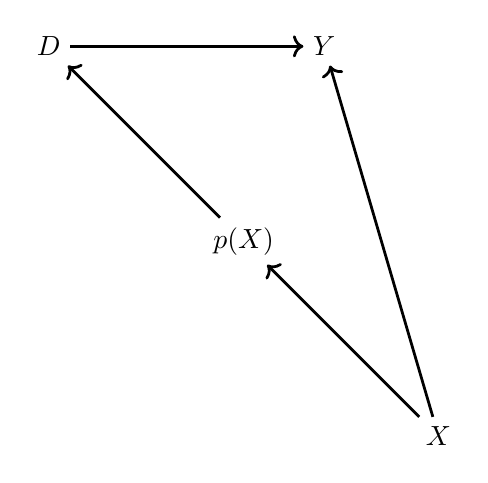
\begin{tikzpicture}
			[node distance=3.5cm]
		% nodes %
		\node[text centered] (d) {$D$};
		\node[below right of = d, text centered] (p) {$p(X)$};
		\node[below right of = p, text centered] (x) {$X$};
		\node[right of = d, text centered] (y) {$Y$};
 
		% edges %
		\draw[->, line width= 1] (d) -- (y);
		\draw[->, line width= 1] (x) -- (p);
		\draw[->, line width= 1] (p) -- (d);
		\draw[->, line width= 1] (x) -- (y);
		\end{tikzpicture}
		\end{center}

It's similar to the visualization of the RDD strategy from earlier except that it achieves common support

\end{frame}


\begin{frame}[plain]
	
	\begin{block}{Propensity score theorem}
	If $(Y^1,Y^0)\independent{D}|X$ (CIA), then $(Y^1,Y^0)\independent{D} | \rho(X)$ where $\rho(X)=Pr(D=1|X)$, the propensity score
	\end{block}
	
	\begin{itemize}
	\item Conditioning on the propensity score is enough to have independence between $D$ and $(Y^1,Y^0)$ (Rosenbaum and Rubin 1983)\\
	 \item Valuable theorem because of dimension reduction and convergence rate issues which can introduce biases
	\item \textbf{Big picture}: You can toss $X$ out if you have $\widehat{\rho}$ because all information from $X$ have been absorbed into $\widehat{\rho}$
	\end{itemize}
\end{frame}

\begin{frame}[plain]
	\begin{center}
	\textbf{Proof}
	\end{center}
	
	\begin{itemize}
	\item Before diving into the proof, first recognize that$$Pr(D=1|Y^0,Y^1\rho(X)) = E[D | Y^0,Y^1,\rho(X)]$$because
		\begin{eqnarray*}
		E[D|Y^0,Y^1,\rho(X)] &=& 1\times Pr(D=1|Y^0,Y^1,\rho(X)) \\
		& & + 0 \times Pr(D=0 | Y^0,Y^1,\rho(X))
		\end{eqnarray*}and the second term cancels out.
		\end{itemize}
\end{frame}

\begin{frame}[plain,shrink=5]
	
	\begin{proof}
	Assume $(Y^1,Y^0)\independent{D}|X$ (CIA).  Then:
		\begin{eqnarray*}
		Pr(D=1 | Y^1,Y^0, \rho(X)) &=& \underbrace{\textcolor{blue}{E[D | Y^1, Y^0, \rho(X)]}}_{ \mathclap{\text{See previous slide}}} \\
		&=&\underbrace{\textcolor{blue}{E} [ E [ D | Y^1,Y^0, \rho(X), X] \textcolor{blue}{| Y^1,Y^0,\rho(X)]}}_{ \mathclap{\text{by LIE}}} \\
		&=&\underbrace{\textcolor{blue}{E} [ E [ D | Y^1,Y^0,X] \textcolor{blue}{| Y^1,Y^0,\rho(X)]}}_{ \mathclap{\text{Given $X$, we know $p(X)$}}} \\
		&=&\underbrace{\textcolor{blue}{E} [E [D | X] \textcolor{blue}{| Y^1,Y^0,\rho(X)]}}_{ \mathclap{\text{by CIA}}} \\
		&=& \underbrace{\textcolor{blue}{E}[\rho(X) \textcolor{blue}{| Y^1, Y^0, \rho(X)]}}_{ \mathclap{\text{propensity score definition}}} \\
		&=& \rho(X)
		\end{eqnarray*}
	\end{proof}
	
\end{frame}

\begin{frame}[plain]
\begin{center}
\textbf{Similar proof}
\end{center}

	 We also can show that the probability of treatment conditional on the propensity score is the propensity score using a similar argument:
		\begin{eqnarray*}
		Pr(D=1| \rho(X)) &=& \underbrace{E[ D | \rho(X) ]}_{\mathclap{\text{Previous slide}}} \\
		&=& \underbrace{E [ E [D | X] | \rho(X)]}_{ \mathclap{\text{LIE}}} \\
		&=& \underbrace{E[p(X) | \rho(X)]}_{ \mathclap{\text{definition}}} \\
		&=& \rho(X)
		\end{eqnarray*}and $Pr(D=1 | Y^1, Y^0, \rho(X)) = Pr(D=1| \rho(X))$ by CIA
\end{frame}


\begin{frame}[plain]
\begin{center}
\textbf{Unbiased estimation of the ATE}
\end{center}

Exact methods to do this to be discussed later, but until then, we can say this:
	\begin{block}{Corollary: Estimating the ATE}
	If $(Y^1,Y^0)\independent{D}|X$, we can estimate average treatment effects:
 $$E[Y^1-Y^0|\rho(X)] = E[Y|D=1,\rho(X)] - E[Y|D=0,\rho(X)]$$
	\end{block}
	
\end{frame}

\begin{frame}[plain]
	\begin{center}
	\textbf{Balancing property}
	\end{center}
	
	\begin{itemize}
	\item Because the propensity score is a function of X, we know:
		\begin{eqnarray*}
		Pr(D=1 | X,\rho(X)) &=& Pr(D=1|X)\\
		&=& \rho(X)
		\end{eqnarray*}
	\item Conditional on $\rho(X)$, the probability that $D=1$ does not depend on $X$.  
	\item $D$ and $X$ are independent conditional on $p(X)$: $$D\independent{X} | \rho(X)$$
	\end{itemize}
\end{frame}


\begin{frame}[plain]
\begin{center}
\textbf{Balancing property}
\end{center}

\begin{itemize}
	\item So we obtain the \textbf{balancing property} of the propensity score: $$Pr(X|D=1,p(X)) = Pr(X|D=0, p(X))$$ conditional on the property score, the distribution of the covariates is the same for treatment and control group units
	\item We can use this to check if our estimated propensity score actually produces balance:$$Pr(X|D=1,\widehat{p}(X)) = Pr(X|D=0, \widehat{p}(X))$$
\end{itemize}

\end{frame}


\begin{frame}[plain]
	\begin{center}
	\textbf{Propensity score theorem}
	\end{center}
	
	\begin{itemize}
	\item This theorem tells us the \emph{only} covariate we need to adjust for is the conditional probability of treatment itself (i.e., the propensity score)
	\item It does not tell us which method we should use to do that adjustment, though, which is an estimation question
	\item There are options: inverse probability weighting, forms of imputation, stratification, and sometimes even regressions will incorporate the score as weights
	\end{itemize}
\end{frame}



\begin{frame}[plain]

	\begin{center}
	\textbf{Checking the common support assumption}
	\end{center}
	
	\begin{itemize}
	\item We can summarize the propensity scores in the treatment and control group and count how many units are off-support
	\item Crump, et al. (2009) offer a rule of thumb: keep scores on interval [0.1,0.9]. 
	\item Tossing out observations beyond those min and max scores
	\item A histogram of propensity scores by treatment and control group also highlights the overlap problem; software also can help such as \texttt{teffects overlap}
	\end{itemize}
	
\end{frame}



\subsection{Inverse probability weighting}

\begin{frame}
\begin{center}
\textbf{Inverse probability weighting}
\end{center}

\begin{itemize}
	\item I really like the simple method of inverse probability weighting aesthetically because there are no black boxes; it's all non-parametric averaging done through a particular kind of weights based on the propensity score
	\item IPW involves fewer implementation choices like number of neighbors, common support, etc.
	\item And because IPW is a smooth estimator, the bootstrap is valid for inference unlike covariate nearest neighbor matching which Abadie and Imbens (2008) show is not valid
\end{itemize}

\end{frame}

\begin{frame}[plain]
\begin{center}
\textbf{Inverse probability weighting}
\end{center}

\begin{itemize}
	\item IPW is basically a reweighting of the outcomes by the propensity score developed in Robins and Rotnitzky (1995), Imbens (2000), Hirano and Imbens (2001)
	\item The weights can be expressed in two ways -- without normalization (Horvitz and Thompson 1952) or normalized (Hajek1971) -- the difference being how well either approach can handle extreme values of the propensity score; the differences come out of the survey sampling literature 
	\item Notation is far far scarier than in fact what we are doing, so I'll show you this in a Stata and R simulation to help pin down the intuition a little better
	\item We'll start with the basic idea using the Horvitz and Thompson (1952) expression of the weights as it's not as messy.
\end{itemize}

\end{frame}
	
	

\begin{frame}[plain]
	\begin{center}
	\textbf{Inverse Probability Weighting}
	\end{center}
	
		\begin{block}{Proposition}
	If $Y^1,Y^0 \independent{D}|X$, then
		\begin{eqnarray*}
		\delta_{ATE}&=&E[Y^1-Y^0] \\
		&=&E \left[ Y \cdot  \frac{D - \rho(X)}{\rho(X) \cdot (1-\rho(X))} \right]\\
		\delta_{ATT}&=&E[Y^1-Y^0|D=1] \\
		&=& \frac{1}{Pr(D=1)} \cdot  E \left[ Y \cdot \frac{D-\rho(X)}{1-\rho(X)} \right]
		\end{eqnarray*}
	\end{block}

\end{frame}

\begin{frame}[plain,shrink=5]
\begin{center}
\textbf{IPW Proof}
\end{center}

	\begin{proof}
	\begin{eqnarray*}
	E \left[ Y \cdot \frac{D-\rho(X)}{\rho(X)(1-\rho(X))} \Big\vert X \right] &=& E \left[ \frac{Y}{\rho(X)} \Big\vert X,D=1 \right] \rho(X) \\
	&& + E\left[ \frac{-Y}{1-\rho(X)} \Big\vert X,D=0 \right](1-\rho(X)) \\
	&=& E[Y|X,D=1] - E[Y|X,D=0]
	\end{eqnarray*}and the results follow from integrating over $P(X)$ and $P(X|D=1)$.
	\end{proof}

\end{frame}


\begin{frame}[plain]
	\begin{center}
	\textbf{Weighting on the propensity score}
	\end{center}

Previous formulas used population concepts. Switching to samples, we use a two-step estimator:
	\begin{enumerate}
	\item Estimate the propensity score: $\widehat{\rho}(X)$
	\item Use estimated score to produce analog estimators. Let $\widehat{\delta}_{ATE}$ and $\widehat{\delta}_{ATT}$  be an estimate of the $ATE$ and $ATT$ parameter:
		\begin{eqnarray*}
		\widehat{\delta}_{ATE} &=& \frac{1}{N} \sum_{i=1}^N Y_i \cdot \frac{D_i - \widehat{\rho}(X_i)}{\widehat{\rho}(X_i) \cdot (1-\widehat{\rho}(X_i))}\\
		\widehat{\delta}_{ATT} &=& \frac{1}{N_T} \sum_{i=1}^N Y_i \cdot \frac{D_i - \widehat{\rho}(X_i)}{1-\widehat{\rho}(X_i)}
		\end{eqnarray*}
	\end{enumerate}
\end{frame}

\begin{frame}[plain]
	\begin{center}
	\textbf{Weighting on the propensity score}
	\end{center}
	
		
Standard errors can be constructed a few different ways:
	\begin{itemize}
	\item We need to adjust the standard errors for first-step estimation of $\rho(X)$
	\item Parameteric first step: Newey and McFadden (1994)
	\item Non-parametric first step: Newey (1994)
	\item Or bootstrap the entire two-step procedure (Adudumilli 2018 and Bodory et al. 2020)
	\end{itemize}
\end{frame}



\begin{frame}[plain]
\begin{center}
\textbf{Implementation with software}
\end{center}

\begin{itemize}
\item I like estimating with IPW manually because I like being reminded how simple a procedure it is
\item But Stata's -teffects- and R's -ipw- do it too, and -teffects- uses the Hajek normalization weights which will produce identical estimates to my program
\item My programs don't do the inference, but I think that would be fun and easy to do using the bootstrap
\item Let's look at it real quickly now with an example from LaLonde's 1986 paper on the NSW job trainings program (which I'll discuss again soon)
\end{itemize}

\end{frame}

\subsubsection{Double robust}
\begin{frame}[plain]
\begin{center}
\textbf{Double robust estimators}
\end{center}

\begin{itemize}
\item Lots of papers: Robins and Rotnizky (1995) originally, Hirano and Imbens (2001), etc.
\item Basic idea is you are going to control for covariates twice: through regression and then through the propensity score
\item We say that estimators combining regression with IPW are double robust so long as
	\begin{itemize}
	\item The regression for the outcome is properly specified, or
	\item The propensity score is properly specified
	\end{itemize}
\item Hence the name ``double robust''. We give ourselves two chances to get it right (either/or not both/and)
\end{itemize}

\end{frame}

\begin{frame}[plain]
\begin{center}
\textbf{Estimation of outcome model}
\end{center}

\begin{eqnarray*}
y_i = \alpha_0 + X_i\beta + \tilde{\alpha_1} D_i + \theta_0 \frac{D_i}{\widehat{\rho (X_i)}} + \theta_1 \frac{1-D_i}{1- \widehat{\rho (X_i)}} + \tilde{\varepsilon_i}
\end{eqnarray*}

\end{frame}

\subsection{Propensity score matching}

\begin{frame}

	\begin{center}
	\textbf{Propensity score matching}
	\end{center}
	
	\begin{itemize}
	\item Matching, or what I like to call ``imputation'', is another way that utilizes the $\widehat{\rho}$
	\item They all use the same first stage, but differ on their second and third stages
	\item Part of the second stage may be imposing common support through ``trimming'', but for different reasons because now this idea of distance is entering and maybe you think some units are ``too far away'' to be relevant counterfactuals
	\end{itemize}

\end{frame}




\begin{frame}[plain]

	\begin{center}
	\textbf{Standard matching strategy}
	\end{center}
	
	\begin{itemize}
	\item Pair each treatment unit $i$ with one or more \emph{comparable} control group unit $j$, where comparability is in terms of proximity to the estimated propensity score
	\item Impute the unit's missing counterfactual outcome $Y_{i(j)}$ based on the unit or units chosen in the previous step
	\item If more than one are ``nearest neighbors'', then use the neighbors' weighted outcomes  $$Y_{i(j)} = \sum_{j \in C(i)} w_{ij}Y_j$$ where $C(i)$ is the set of neighbors with $W=0$ of the treatment unit $i$and $w_{ij}$ is the weight of control group units $j$ with $\sum_{j \in C(i)} w_{ij} = 1$
	\end{itemize}
\end{frame}


\begin{frame}[plain]

	\begin{center}
	\textbf{Imputing the counterfactuals}
	\end{center}
	
	A parameter of interest: $$E[Y^1_i | D_i=1] - E[Y^0_i | D_i=1]$$We estimate it as follows  $$\widehat{ATT} = \frac{1}{N_T} = \sum_{i:W_i=1} \bigg [Y_i - Y_{i(j)} \bigg ]$$where $N_T$ is the number of matched treatment units in the sample. Note the difference between \emph{imputation} and weighting

\end{frame}

\begin{frame}[plain]
	\begin{center}
	\textbf{Matching methods}
	\end{center}
	
	\begin{itemize}
	\item The probability of observing two units with \emph{exactly} the same propensity score is in principle zero because $p(x)$ is continuous
	\item Several matching methods have been proposed in the literature, but the most widely used are:
		\begin{itemize}
		\item Stratification matching
		\item Nearest-neighbor matching (with or without caliper)
		\item Radius matching
		\item Kernel matching
		\end{itemize}
	\item Typically, one treatment unit $i$ is matched to several control units $j$, but sometimes one-to-one matching is used
	\end{itemize}
	
\end{frame}


\begin{frame}[plain]

	\begin{center}
	\textbf{Stratification}
	\end{center}
	
	\begin{itemize}
	\item Stratification is used to force covariate balance by finding strata where there is no difference in mean covariate values. 
	\item You then use those strata to calculate within differences in means and sum over properly weighted strata. See Becker and Ichino (2002)
	\item  Stratification is a brute force method for imposing balance by grouping the data and testing for differences in covariate means
	\item It's actually kind of similar to coarsened exact matching, only using the propensity score for the ``stratification'' not the covariates
	\end{itemize}
	
\end{frame}


\begin{frame}[plain]

	\begin{center}
	\textbf{Stratification: Achieving Balance}
	\end{center}
	
The algorithm is brute force covariate balancing
	\begin{enumerate}
		\item Sort the data by propensity score and divide into groups of observations with similar propensity scores (e.g., percentiles)
		\item Within each group, test (using a t-test) whether the means of the covariates ($X$) are equal between treatment and control
		\item If so, then stop.  If not, it means the covariates aren't balanced \emph{within that group}.  Divide the group in half and repeat
		\item If a particular covariate is unbalanced for multiple groups, modify the initial logit or probit equation by including higher order terms and/or interactions with that covariate and repeat
		\end{enumerate}
Historically this could be done with -\texttt{pscore2.ado}- or manually oneself if they felt so inclined, but it was dropped with -\texttt{teffects}-
\end{frame}


\begin{frame}[plain]

	\begin{center}
	\textbf{Nearest Neighbor}
	\end{center}
	
	Pretty similar to covariate matching.  Formula is $$ATT^{NN} = \frac{1}{N_T} \sum_{i:W_i=1} \bigg [ Y_i - \sum_{j \in C(i)_M} w_{ij}Y_j \bigg ]$$ 
		\begin{itemize}
		\item $N_T$ is the number of Treatment units $i$
		\item $w_{ij}$ is equal to $\frac{1}{N_C}$ if $j$ is a control unit and zero otherwise; $N_C$ is number of control units $j$
		\item And unit $j$ is chosen as a control for $i$ if it's propensity score is nearest to that of $i$
		\end{itemize}
\end{frame}

\begin{frame}[plain]
	
	\begin{center}
	\textbf{NN Matching: Bias vs. Variance}
	\end{center}
	
	\begin{itemize}
	\item But how far away on the propensity score will you use? Herein lies the different types of matching proposed
		\begin{itemize}
		\item Matching just one nearest neighbor minimizes bias at the cost of larger variance
		\item Matching using additional nearest neighbors increases the bias but decreases the variance
		\end{itemize}
	\item Matching with or without replacement
		\begin{itemize}
		\item with replacement keeps bias low at the cost of larger variance
		\item without replacement keeps variance low but at the cost of potential bias
		\end{itemize}
	\end{itemize}
	
\end{frame}


\begin{frame}[plain]
\begin{center}
\textbf{Distance between treatment and control units}
\end{center}

\begin{itemize}
\item What was historically done was limiting ``distance''  through various \emph{ad hoc} choices
\item Imagine these choices as creating like a lasso (like the cowboy rope)
\item Anything within the lasso could be used for the imputation; anything outside the lasso could not
\item There were two common ways -- caliper matching and radius matching. 
\end{itemize}

\end{frame}

\begin{frame}[plain]

	\begin{center}
	\textbf{Caliper matching}
	\end{center}
	
	\begin{itemize}
	\item Caliper matching is a variation on NN matching that tries to build brakes into the algorithm as to avoid ``bad neighbors''
	\item It does this by imposing a tolerable maximum distance (e.g., 0.2 units in the propensity score away from a treatment unit $i$'s propensity score)
	\item Note -- this is a one-to-one imputation, and if there doesn't exist anybody in the control group unit $j$ within that ``caliper'', then treatment unit $i$ is discarded
	\item Means we aren't estimating the ATE anymore once we start dropping units
	\item It's difficult to know what this caliper should be \emph{ex ante}, hence why I said it is somewhat \emph{ad hoc}
	\end{itemize}

\end{frame}


\begin{frame}[plain]

	\begin{center}
	\textbf{Radius matching}
	\end{center}
	
	
		\begin{itemize}
		\item Each treatment unit $i$ is matched with the control group units whose propensity score are in a predefined neighborhood of the propensity score of the treatment unit.
		\item \textbf{All} the control units with $\widehat{\rho_j}$ falling within a radius $r$ from $\widehat{\rho}_i$ are matched to the treatment unit $i$ -- this is what distinguishes it from calipers, and makes it more similar to covariate matching (Abadie and Imbens 2006, 2008)
		\item The smaller the radius, the better the quality of the matches, but the higher the possibility some treatment units are not matched because the neighborhood does not contain control group units $j$
		\end{itemize}
		
\end{frame}

\begin{frame}[plain]
\begin{center}
\textbf{Software}
\end{center}

\begin{itemize}
\item I think you can use -\texttt{teffects, psmatch}- to get at these two nearest neighbor approaches by setting the number of matches
\item You can use -\texttt{pscore2}- for stratification, but I think the standard errors are wrong, so you may need to just do it manually using bootstrapping or variance approximation, and that may be a pain to program up
\item Not sure of the R command, but I know it's out there
\end{itemize}

\end{frame}


\begin{frame}[plain]

	\begin{center}
	\textbf{King and Nielsen (2019)}
	\end{center}
	
	\begin{itemize}
	\item There is a King and Nielsen (2019) critique of these methods that is popularly known but not popularly studied
	\item King and Nielsen (2019) is not a critique of the propensity score, because it does not apply to stratification, regression adjustment, or inverse probability weighting
	\item It only applies to nearest neighbor and is related to forced balance through trimming and a myriad of other common choices made by the researcher
	\end{itemize}
	
\end{frame}

\begin{frame}[plain]

\begin{quote}
	

```[The] more balanced the data, or the more balance it becomes by [trimming] some of the observations through matching, the more likely propensity score matching will degrade inferences.'' -- King and Nielsen (2019)

\end{quote}
	
\end{frame}


\begin{frame}[plain]
	\begin{center}
	\textbf{Examples of propensity score matching}
	\end{center}
	
	\begin{itemize}
	\item Workhorse example of propensity score matching is the Job Trainings Program (NSW) 
	\item First studied by LaLonde (1986) evaluating multiple econometric models for program evaluation 
		\begin{itemize}
		\item All the standard estimators failed to estimate the known ATE when replacing experimental controls with non-experimental controls -- even difference-in-differences
		\end{itemize}
	\item Dehejia and Wahba (1999; 2002) use LaLonde's data with propensity score matching and found better results
	\item Critiques by Petra Todd, Jeff Smith and others followed which I won't review here for sake of time
	\end{itemize}
\end{frame}



\begin{frame}[plain]
	\begin{center}
	\textbf{Description of NSW Job Trainings Program}
	\end{center}
	
The National Supported Work Demonstration (NSW), operated by Manpower Demonstration Research Corp in the mid-1970s:
	\begin{itemize}
	\item was a temporary employment program designed to help disadvantaged workers lacking basic job skills move into the labor market by giving them work experience and counseling in a sheltered environment
	\item was also unique in that it \textbf{randomly assigned} qualified applicants to training positions:
		\begin{itemize}
		\item \textbf{Treatment group}: received all the benefits of NSW program
		\item \textbf{Control group}: left to fend for themselves
		\end{itemize}
	\item admitted AFDC females, ex-drug addicts, ex-criminal offenders, and high school dropouts of both sexes
	\end{itemize}
\end{frame}

\begin{frame}[plain]
	\begin{center}
	\textbf{NSW Program}
	\end{center}
	
	\begin{itemize}
	\item Treatment group members were:
		\begin{itemize}
		\item guaranteed a job for 9-18 months depending on the target group and site
		\item divided into crews of 3-5 participants who worked together and met frequently with an NSW counselor to discuss grievances and performance
		\item paid for their work
		\end{itemize}
	\item Control group members were randomized so the same
	\item Note: the randomization balanced observables and unobservables across the two arms, thus enabling the estimation of an ATE for the people who self-selected into the program
	\end{itemize}
\end{frame}

\begin{frame}[plain]
\begin{center}
\textbf{NSW Program}
\end{center}

\begin{itemize}
	\item Other details about the NSW program:
		\begin{itemize}
		\item \underline{Wages}:  NSW offered the trainees lower wage rates than they would've received on a regular job, but allowed their earnings to increase for satisfactory performance and attendance
		\item \underline{Post-treatment}: after their term expired, they were forced to find regular employment
		\item \underline{Job types}:  varied within sites -- gas station attendant, working at a printer shop -- and males and females were frequently performing different kinds of work
		\end{itemize}
\end{itemize}

\end{frame}
	
\begin{frame}[plain]
	\begin{center}
	\textbf{NSW Data}
	\end{center}
	
	\begin{itemize}
	\item \underline{NSW data collection}:
		\begin{itemize}
		\item MDRC collected earnings and demographic information from both treatment and control at baseline and every 9 months thereafter
		\item Conducted up to 4 post-baseline interviews
		\item Different sample sizes from study to study can be confusing, but has simple explanations
		\end{itemize}
	\end{itemize}
\end{frame}
	

\begin{frame}[plain]
\begin{center}
\textbf{NSW Data}
\end{center}

\begin{itemize}
	\item \underline{Estimation}:
		\begin{itemize}
		\item NSW was a randomized job trainings program; therefore estimating the average treatment effect is straightforward:
			\begin{eqnarray*}
			\frac{1}{N_t}\sum_{D_i=1}Y_i - \frac{1}{N_c}\sum_{D_i=0}Y_i \approx E[Y^1-Y^0] 
			\end{eqnarray*}in large samples assuming treatment selection is independent of potential outcomes (randomization) -- i.e., $(Y^0,Y^1)\independent{D}$. 
		\end{itemize}
	\item \underline{NSW worked}: Treatment group participants' real earnings post-treatment (1978) was positive and economically meaningful -- $\approx$ \$900 (LaLonde 1986) to \$1,800 (Dehejia and Wahba 2002) depending on the sample used
\end{itemize}

\end{frame}
	
\begin{frame}[plain]
	\begin{center}
	LaLonde, Robert J. (1986). \myurlshort{http://business.baylor.edu/scott_cunningham/teaching/lalonde-1986.pdf}{``Evaluating the Econometric Evaluations of Training Programs with Experimental Data''}. \emph{American Economic Review}. 
	\end{center}
	
\underline{LaLonde's study} was \textbf{not} an evaluation of the NSW program, as that had been done, but rather an evaluation of econometric models done by:
		\begin{itemize}
		\item replacing the experimental NSW control group with non-experimental control group drawn from two nationally representative survey datasets: Current Population Survey (CPS) and Panel Study of Income Dynamics (PSID)
		\item estimating the average effect using non-experimental workers as controls for the NSW trainees 
		\item comparing his non-experimental estimates to the experimental estimates of \$900
		\end{itemize}
\end{frame}

\begin{frame}[plain]
\begin{center}
\textbf{LaLonde (1986)}
\end{center}

\begin{itemize}

	\item \underline{LaLonde's conclusion}: available econometric approaches were biased and inconsistent
		\begin{itemize}
		\item His estimates were way off and usually the wrong sign
		\item Conclusion was influential in policy circles and led to greater push for more experimental evaluations
		\end{itemize}

\end{itemize}

\end{frame}

\begin{frame}[plain]
	\begin{figure}
	\includegraphics[scale=0.8]{./lecture_includes/lalonde_table5a.png}
	\end{figure}

\end{frame}
\begin{frame}[plain]
	\begin{figure}
	\includegraphics[scale=0.8]{./lecture_includes/lalonde_table5b.png}
	\end{figure}

\end{frame}

\begin{frame}[plain,shrink=10]
	\begin{center}
	\textbf{Imbalanced covariates for experimental and non-experimental samples}
	\end{center}

		\begin{center}
		\begin{table}
		\begin{tabular}{lcccccc}
		\hline \hline
		\multicolumn{3}{c}{}&
		\multicolumn{1}{c}{CPS}&
		\multicolumn{1}{c}{NSW}\\
		
		\multicolumn{1}{c}{}&
		\multicolumn{2}{c}{All} &
		\multicolumn{1}{c}{Controls} &
		\multicolumn{1}{c}{Trainees} \\

		\multicolumn{3}{c}{}&
		\multicolumn{1}{c}{$N_c=15,992$}&
		\multicolumn{1}{c}{$N_t=297$}&
		\multicolumn{1}{c}{}&
		\multicolumn{1}{c}{}\\

		\multicolumn{1}{l}{covariate}&
		\multicolumn{1}{c}{mean}&
		\multicolumn{1}{c}{(s.d.)}&
		\multicolumn{1}{c}{mean}&
		\multicolumn{1}{c}{mean}&
		\multicolumn{1}{c}{t-stat}&
		\multicolumn{1}{c}{diff}\\
		\hline
Black    & 0.09 & 0.28 & 0.07 & 0.80 & 47.04 & -0.73\\
Hispanic & 0.07 & 0.26 & 0.07 & 0.94 & 1.47 & -0.02\\
Age & 33.07 & 11.04 & 33.2 & 24.63 & 13.37  & 8.6\\
Married & 0.70 & 0.46 & 0.71 & 0.17 & 20.54 & 0.54\\
No degree & 0.30 & 0.46 & 0.30 & 0.73 & 16.27 & -0.43\\
Education & 12.0 & 2.86 & 12.03 & 10.38 & 9.85 & 1.65 \\
1975 Earnings   & 13.51 & 9.31 & 13.65 & 3.1 & 19.63 & 10.6\\
1975 Unemp  & 0.11 & 0.32 & 0.11 & 0.37 & 14.29 & -0.26\\
		\hline 
		\end{tabular}
		\end{table}
		\end{center}

\end{frame}


\begin{frame}[plain]
	\begin{center}
	\textbf{Dehija and Wahba (1999)}
	\end{center}
	
	\begin{itemize}
	\item Dehejia and Wahba (DW) update LaLonde's original study using propensity score matching
		\begin{enumerate}
		\item Dehejia, Rajeev H. and Sadek Wahba (1999). 	``Causal Effects in Nonexperimental Studies: Reevaluating the Evaluation of Training Programs''. \underline{Journal of the American Statistical} \underline{Association}, vol. 94(448): 1053-1062 (\myurlshort{http://business.baylor.edu/scott_cunningham/teaching/dehejia-and-wahba-1999.pdf}{pdf})
		\end{enumerate}
	\item Can propensity score matching improve over the estimators that LaLonde examined?
	\end{itemize}
\end{frame}

\begin{frame}[plain]
	
\begin{figure}
\includegraphics[scale=0.5]{./lecture_includes/dw_1.pdf}
\end{figure}

\end{frame}

\begin{frame}[plain]

\begin{figure}
\includegraphics[scale=0.5]{./lecture_includes/dw_2.pdf}
\end{figure}


\end{frame}

\begin{frame}[plain]

	\begin{center}
	\textbf{Proposition 2}
	\end{center}
	
	\begin{eqnarray*}
	X \independent D | p(X)
	\end{eqnarray*}
	
	\begin{itemize}
	\item Conditional on the propensity score, the covariates are independent of the treatment, suggesting that the distribution of covariate values should be the same for both treatment and control groups
	\item This can be checked as we have data on all three once we've estimated the propensity score
	\end{itemize}

\end{frame}

\begin{frame}[plain]

	\begin{center}
	\textbf{Trimming the data}
	\end{center}
	
	\begin{itemize}
	\item Common terms are ``trimming'' or ``pruning''
	\item Drop units which do not overlap in terms of estimated propensity score
	\item Sometimes as a rule of thumb, just keep units on the \texttt{[0.1,0.9]} interval
	\end{itemize}

\end{frame}


\begin{frame}[plain]

	\begin{center}
	\textbf{Common support}
	\end{center}
	
\centering
  \begin{overprint}%
\begin{figure}[h]
  \makebox[\textwidth][c]{\includegraphics[width=1.2\textwidth]{./lecture_includes/dw_3.pdf}}%
\end{figure}
  \end{overprint}%

\end{frame}



\begin{frame}[plain]

	\begin{center}
	\textbf{Overlap}
	\end{center}

\begin{figure}
  \makebox[\textwidth][c]{\includegraphics[width=1.2\textwidth]{./lecture_includes/dw_4.pdf}}%
\end{figure}

\end{frame}

\begin{frame}[plain]

	\begin{center}
	\textbf{Results}
	\end{center}
	
\begin{figure}[h]
  \makebox[\textwidth][c]{\includegraphics[width=1.2\textwidth]{./lecture_includes/dw_5.pdf}}%
\end{figure}

\end{frame}

\begin{frame}[plain]

	\begin{center}
	\textbf{Covariate balance}
	\end{center}

\begin{figure}[h]
  \makebox[\textwidth][c]{\includegraphics[width=1.2\textwidth]{./lecture_includes/dw_6.pdf}}%
\end{figure}


\end{frame}


\begin{frame}[plain]
	\begin{center}
	\textbf{Estimation in Stata}
	\end{center}
	
	\begin{itemize}
	\item I have written up code that will implement IPW on the DW data
	\item It's nonparametric, so it doesn't use any packages
	\item But you are welcome to try some packages, particularly the -\texttt{teffects}- command
	\end{itemize}
	
\end{frame}



\begin{frame}[plain]
	\begin{center}
	\textbf{Kernel matching}
	\end{center}
	
	\begin{itemize}
	\item Alternatively we can perform propensity score matching with a kernel-based method. 
	\item Notice on the next slide that the estimate of the ATT switches sign relative to that produced by the NN matching algorithm
	\end{itemize}
\end{frame}


\begin{frame}[plain]
\begin{center}
\textbf{Stata syntax}
\end{center}

\lstinputlisting{./lecture_includes/score2.do} 
\end{frame}


\begin{frame}[plain]

	\begin{figure}
  \makebox[\textwidth][c]{\includegraphics[width=1.2\textwidth]{./lecture_includes/ps_output3.png}}%
	\end{figure}


\end{frame}

\begin{frame}[plain]

	\begin{figure}
  \makebox[\textwidth][c]{\includegraphics[width=1.2\textwidth]{./lecture_includes/ps_output4.png}}%
	\end{figure}


\end{frame}

\begin{frame}[plain]

	\begin{center}
	\textbf{Matchings vs. Propensity score}
	\end{center}
	
	\begin{figure}
  \makebox[\textwidth][c]{\includegraphics[width=1.2\textwidth]{./lecture_includes/abadie-imbens-2011.pdf}}%
	\end{figure}



\end{frame}


\clearpage
\newpage

\begin{frame}[plain]
\begin{center}
\textbf{Subsequent studies}
\end{center}

\begin{itemize}
\item Heckman et al. (1996, 1998) used experimental data from the US National Job Training Partnership Act (JTPA)
\item They conclude that in order for matching estimators to have low bias, it is important that the data include a rich set of variables related to program participation and labor market outcomes, that the nonexperimental comparison group be drawn from the same local labor markets as the participants and the dependent variable (typically earnings) be measured in the same way for participants and nonparticipants
\item All three of these conditions fail to hold in DW (1999, 2002) according to Smith and Todd (2005)
\end{itemize}

\end{frame}


\begin{frame}[plain]
\begin{center}
\textbf{Smith and Todd}
\end{center}

\begin{itemize}
\item Difference-in-differences with propensity scores tended to work well in Smith and Todd (2005)
\item But hard to make this a rule, because it's hard to know ex ante if we've specified the propensity score correctly (i.e., have CIA)
\item It is vital you know you're data, if you're going to use these methods, which means understanding at a deep level the way in which selection (i.e., treatment assignment) works in your data
\end{itemize}

\end{frame}
\begin{frame}[plain]
\begin{center}
\textbf{Beating a dead horse}
\end{center}

\begin{itemize}
	\item The propensity score can make groups comparable \textbf{but} only on the variables used to estimate the propensity score in the first place.  There is \textbf{NO} guarantee you are balancing on unobserved covariates.
	\item If you know that there are important unobservable variables, you may need another tool.
	\item Remember: randomization ensure that both observable and \textbf{unobservable} variables are balanced
\end{itemize}
\end{frame}


\subsection{Coarsened exact matching}



\begin{frame}
	\begin{center}
	\textbf{Coarsened exact matching}
	\end{center}

	
\begin{itemize}
\item There are two kinds of matching as we've said
	\begin{enumerate}
	\item \emph{Exact matching} matches a treated unit to all of the control units with the same covariate value. Sometimes this is impossible (e.g., continuous covariate). 
	\item \emph{Approximate matching} specifies a metric to find control units that are close to the treated unit. Requires a distance metric, such as Euclidean, Mahalanobis, or the propensity score.  All of which can be implemented in Stata's \texttt{teffects}.
	\end{enumerate}
\item 	Iacus, King and Porro (2011) propose another version of matching they call coarsened exact matching (CEM). Some big picture ideas
\end{itemize}
\end{frame}

\begin{frame}[plain]
\begin{center}
\textbf{Checking imbalance}
\end{center}

\begin{itemize}
\item Iacus, King and Porro (2008) say that in practice approximate matching requires setting the matching solution beforehand, then checking for imbalance after.  
\item Start over, repeat, until the user is exhausted by checking for imbalance.
\end{itemize}

\end{frame}

\begin{frame}[plain]
	\begin{center}
	\textbf{CEM Algorithm}
	\end{center}
	
\begin{enumerate}
\item Begin with covariates $X$. Make a copy called $X*$
\item Coarsen $X*$ according to user-defined cutpoints or CEM's automatic binning algorithm
	\begin{itemize}
	\item Schooling $\rightarrow$ less than high school, high school, some college, college, post college
	\end{itemize}
\item Create one stratum per unique observation of $X*$ and place each observation in a stratum
\item Assign these strata to the original data, $X$, and drop any observation whose stratum doesn't contain at least one treated and control unit
\end{enumerate}

You then add weights for stratum size and analyze without matching.

\end{frame}

\begin{frame}[plain]
	\begin{center}
	\textbf{Tradeoffs}
	\end{center}
	
	\begin{itemize}
	\item Larger bins mean more coarsening.  This results in fewer strata.  
	\item Fewer strata result in more diverse observations within the same strata and thus higher imbalance
	\item CEM prunes both treatment and control group units, which changes the parameter of interest.  Be transparent about this as you're not estimating the ATE or the ATT when you start pruning
	\end{itemize}
	
\end{frame}

\begin{frame}[plain]
	\begin{center}
	\textbf{Benefits}
	\end{center}
	
	\begin{itemize}
	\item The key benefit of CEM is that it is in a class of matching methods called \emph{monotonic imbalance bounding}
	\item MIB methods bound the maximum imbalance in some feature of the empirical distributions by an ex ante decision by the user
	\item In CEM, this ex ante choice is the coarsening decision
	\item By choosing the coarsening beforehand, users can control the amount of imbalance in the matching solution
	\item It's also wicked fast.
	\end{itemize}
\end{frame}


\begin{frame}[plain]
	\begin{center}
	\textbf{Imbalance}
	\end{center}
	
	\begin{itemize}
	\item There are several ways of measuring imbalance, but here we focus on the $\mathcal{L}_1(f,g)$ measure which is$$\mathcal{L}_1(f,g) = \frac{1}{2} \sum_{l_1 \dots l_k} | f_{l_1 \dots l_k} - g_{l_1 \dots l_k} |$$where the $f$ and $g$ record the relative frequencies for the treatment and control group units.
	\item Perfect global imbalance is indicated by $\mathcal{L}_1=0$.  Larger values indicate larger imbalance between the groups, with a maximum of $\mathcal{L}_1=1$. 
	\end{itemize}
\end{frame}

\begin{frame}[plain]
	\begin{center}
	\textbf{Stata}
	\end{center}
	
	\begin{itemize}
	\item Download $\texttt{cem}$ from Stata:  \texttt{ssc install cem, replace}
	\item You will automatically compute the global imbalance measure, as well as several unidimensional measures of imbalance, when using $\texttt{cem}$
	\item I got a $\mathcal{L}_1=0.55$.  What does it mean?
		\begin{itemize}
		\item By itself, it's meaningless.  It's a reference point between matching solutions.
		\item Once we have a matching solution, we will compare its $\mathcal{L}_1$ to 0.55 and gauge the increase in balance due to the matching solution from that difference.
		\item Thus $\mathcal{L}_1$ works for imbalance as $R^2$ works for model fit: the absolute values mean less than comparisons between matching solutions.
		\end{itemize}
	\end{itemize}
	
\end{frame}

\begin{frame}[plain]
	\begin{center}
	\textbf{More Stata}
	\end{center}
	
	\begin{itemize}
	\item Because $\texttt{cem}$ bounds the imbalance ex ante, the most important information in the Stata output is the number of observations matched.
	\item You can also choose the coarsening as opposed to relying on the algorithm's automated binning.  
	\item Once you have estimated the strata, you regress the outcome onto the treatment and then weight the regression by $\texttt{cem_weights}$.  For instance, $$\texttt{regress re78 treat [iweight=cem\_weight]}$$
	\item For more on this, see Blackwell, et al. Stata journal article from 2009.  
	\end{itemize}
\end{frame}


\section{Concluding remarks}

\subsection{Good luck and have fun}

\begin{frame}
\begin{center}
\textbf{The credibility revolution won}
\end{center}

\begin{itemize}
\item People like Heckman, Rubin, Ashenfelter, LaLonde, Angrist, Krueger, Card, Imbens, Athey, Duflo, Abadie and many others built on their backs a movement of sorts
\item The movement tried to shift economists and other social scientists away from naive empirical methods that couldn't hope to estimate behavioral causal parameters towards things that might
\item It's in your best interest to study empirical methods, papers that use them, how they communicate their findings and the econometricians so that you can be ready when the opportunity arises
\end{itemize}

\end{frame}


\begin{frame}[plain]
\begin{center}
\textbf{Make the stone stoney again}
\end{center}

\begin{itemize}
\item A man walks up the mountain barefoot til he can't feel his feet again -- Victor Schlosskey said art is there to make ``the stone feel like a stone again''. I want research to feel like research again for you
\item Research is a quest for honest answers to good faith questions that people care about
\item Most of all, research is truly fun for those who find such things fun.  It's a form of self-expression and creativity for many of us
\item And it is fun to understand the answers you get and why those answers are reliable which requires checklists, workflows, clearly defined assumptions and proper tools for the job
\item It is not fun to get a bad answer to a poorly defined question that you're not confident about
\end{itemize}

\end{frame}



\begin{frame}[plain]
	\begin{center}
	\textbf{A Priori Knowledge is Necessary for Identification}
	\end{center}
	
	\begin{itemize}
	\item Think hard about these questions: 
		\begin{itemize}
		\item Can you write down a DAG or otherwise model the data generating process?
		\item What parameter do you think is interesting (e.g., ATT, LATE)
		\item What are the assumptions needed for identifying that parameter?
		\end{itemize}
	\item Pick estimators based on these questions, not the other way around
	\item Less so, pick data based on these questions, not the other way around (usually)
	\end{itemize}
\end{frame}


\begin{frame}[plain]
	\begin{center}
	\textbf{What's a good research design?}
	\end{center}
	
	\begin{itemize}
	\item A good research design is one you are excited to tell people about -- that's basically what characterizes \emph{all} research designs, whether propensity score matching or regression discontinuity designs
	\item Don't get enamored by statistical modeling that obscures the identification problem from plain sight.  
	\item Always understand what assumptions you \emph{must} make, be clear which parameters you are and are not identifying
	\item Good research designs help you believe and not be afraid of your answers
	\end{itemize}
\end{frame}



\begin{frame}[plain]
\begin{center}
\textbf{What's the reason for your work?}
\end{center}

\begin{itemize}
\item Causal identification is a necessary but not a sufficient condition for publishing well these days bc the credibility revolution won
\item Must also be an ``interesting'' question - admittedly subjective
\item If it must be interesting, then the best thing you can do for yourself is choose a topic that you care about
\item Publishing is simply too difficult to be working on something you find trivial
\end{itemize}

\end{frame}

\begin{frame}[plain]
\begin{center}
\textbf{Free disposal advice}
\end{center}

\begin{itemize}
\item My colleague said ``a good study and a bad study take the same amount of time'' -- don't work on stuff just to work on it
\item Finding projects with upside, in a set of potential projects, is a good idea
\item The sooner you can cut bait on a bad project and move on, the better -- beware the sunk cost fallacy
\item For my personality, questions are practically existential quests for the meaning of life, but not everyone needs extreme incentives
\item So know yourself, work to your strengths, figure out things that downplay your weaknesses, believe in yourself, find your sponsors and mentors, seek help
\end{itemize}

\end{frame}


\end{document}





\subsection{Imperfect synthetic controls}

\begin{frame}
\frametitle{Background}

\begin{itemize}
\item David Powell, ``Imperfect Synthetic Controls: Did the Massachusetts Health Care Reform Save Lives?'', working paper 2018 \url{https://papers.ssrn.com/sol3/papers.cfm?abstract_id=3192710}
\item Comparative case studies are program evaluation methods when there is only one treatment unit
\item Explicit counterfactuals generated from a set of untreated donor pools
\item The synthetic control method (SCM) developed by Abadie and coauthors (2003, 2010, 2015) is an algorithmic way of ``optimally'' selecting weighted control units 
\item Athey and Imbens have described it as the most important innovation in causal inference of the last 15 years
\end{itemize}

\end{frame}


\begin{frame}
\frametitle{Identifying assumptions}

\begin{itemize}
\item SCM has two main assumptions:
	\begin{enumerate}
	\item convex hull assumtion
	\item perfect
	\end{enumerate}
\item If these do not credibly hold in the data you're using, then SCM is not the method for you

\end{itemize}

\end{frame}

\begin{frame}
\frametitle{Convex hull assumption}

\begin{itemize}
\item Outcomes:
\begin{equation}
Y_{it} = \alpha_{it}D_{it} + \lambda_t \mu_i + \varepsilon_{it}
\end{equation}
\item The convex hull assumption in words states that there exists a set of control group units which when weighted approximate the factor loading of the treatment unit $\mu_{1t}$
\begin{equation}
\sum_{j=2}^Nw_j^1 \mu_{jt} = \mu_{1t}
\end{equation}
\item We do not observe $\mu_i$, so typically we use the noisier measure of $Y_{it}$ instead
\end{itemize}
\end{frame}

\begin{frame}
\frametitle{``Perfect''}
\begin{itemize}
\item Notice the $t$ subscript - the assumption is that the synthetic control approximates the treatment unit \emph{consistently} over long stretches of time (the longer the pre-treatment time series, the more convincing the convex hull assumption holds)
\item This is violated when there are transitory shocks, which is quite common in practice

\end{itemize}

\end{frame}

\begin{frame}
\frametitle{Placebo convex hull assumption}

\begin{itemize}
\item Powell's innovative method finds a way to recover the treatment effect when the convex hull does not hold or does not hold perfectly
\item This requires a new identifying assumption which I'll call the placebo convex hull assumption
\item Basically, imagine estimating synth for the entire sample - treatment and placebos. So long as the following holds
\begin{equation}
\sum_{j\neq i}^N w_j^i \mu_j = \mu_i
\end{equation} for some $i$ with $w_1^i>0$, then the treatment effect can still be calculated
\end{itemize}

\end{frame}

\begin{frame}
\frametitle{Placebo convex hull (cont.)}

\begin{itemize}

\item In words, suppose that Georgia receives some treatment, but for whatever reason, the convex hull assumption won't hold (i.e., Georgia is ``unusual''). Then SCM is not appropriate
\item What Powell shows, though, is that if Georgia appears in the synthetic control for Texas (i.e., $w_{GA}^{TX}>0$), then it is possible to recover the treatment effect through a backdoor procedure
\item What this practically means is estimating the synthetic control model for \emph{all} panel units and determining if Georgia ever receives a positive weight.

\end{itemize}
\end{frame}

\begin{frame}
\frametitle{Placebo convex hull (cont.)}

\begin{eqnarray*}
Y_{it} - \sum_{j \neq i}^N w_j^i Y_{jt} &=& \lambda_t \bigg ( \mu_i - \sum_{j \neq i}^N w_j^i \mu_j \bigg)  + \bigg (\alpha_{it} D_{it} - \sum_{j \neq i}^N w_j^i \alpha_{jt} D_{jt} \bigg ) \\
&&+ \bigg (\varepsilon_{it} - \sum_{j \neq i}^N w_j^i \varepsilon_{jt} \bigg )
\end{eqnarray*}

\begin{itemize}
\item The first term is equal to zero by the placebo convex hull assumption
\item The second term collapses to $-\alpha_{1t} w_1^i$ for the treatment unit $(D=1)$ and for positive weights $w_1^i>0$
\end{itemize}

\end{frame}

\begin{frame}
\frametitle{Placebo convex hull (cont.)}

\begin{eqnarray*}
Y_{it} - \sum_{j \neq i}^N w_j^i Y_{jt} &=& - \alpha_{1t} w_1^i + \bigg (\varepsilon_{it} - \sum_{j \neq i}^N w_j^i \varepsilon_{jt} \bigg )
\end{eqnarray*}

\begin{itemize}
\item For identifying $\alpha_{1t}$ Powell proposes estimating with WLS
\begin{equation}
\dddot{Y} = \alpha_1 \dddot{D} + \dddot{\varepsilon}
\end{equation}where \begin{eqnarray*}\dddot{Y} &=& Y_{it} - \sum_{j \neq i} \widehat{w}_j^i Y_{jt} \\
\dddot{D} &=& D_{it} - \sum_{j \neq i} \widehat{w}_j^i D_{jt} \\
\dddot{\varepsilon} &=& \varepsilon_{it} - \sum_{j \neq i} w_j^i \varepsilon_{jt} 
\end{eqnarray*}
\end{itemize}


\end{frame}

\begin{frame}
\frametitle{Weighted least squares}

\begin{itemize}
\item Powell suggests using weighted least squares to estimate equation (4) where the weights are the variance on each $i$ difference in pre-treatment outcomes to its synthetic control
\begin{eqnarray*}
\widehat{V}_i = \frac{1}{T_0} \sum_{t=1}^{T_0} \bigg ( Y_{it} - \sum_{j \neq i}^N \widehat{w}_j^i Y_{jt} \bigg )^2
\end{eqnarray*}
\item This final regression includes all units which are then weighted by $\frac{1}{\widehat{V}_i}$.  
\item This intrinsically upweights those units with better fit and downweights those with poor fit
\end{itemize}

\end{frame}

\begin{frame}
\frametitle{Implementation}

\begin{itemize}
\item If I'm following correctly, the steps are as follows:
\begin{enumerate}
\item Estimate synth for all units (not sure about model selection)
\item Store counterfactuals and merge with main dataset
\item Estimate differences for outcomes and treatments per panel unit time
\item Estimate variance (time invariant weight)
\item Estimate weighted least squares
\end{enumerate}
\item I think this is going to involve mainly programmed loops, storage and merges. Just needs synth
\end{itemize}
\end{frame}

\begin{frame}
\frametitle{Commentary about alternative assumption}

\begin{itemize}
\item I'd like to focus on the identifying assumption
\begin{eqnarray*}
Y_{it} - \sum_{j \neq i}^N w_j^i Y_{jt} &=& \lambda_t \bigg ( \mu_i - \sum_{j \neq i}^N w_j^i \mu_j \bigg)  +  \dots
\end{eqnarray*}
\item Does this mean that the placebo convex hull assumption must hold for all $i$?
\item If so, how is this possible?  I can imagine a situation where the assumption held for some unit $i$ but not for all unit $i$ in other words. Placebo synthetic controls often have wild outliers with poor pre-treatment fit
\end{itemize}
\end{frame}

\begin{frame}
\frametitle{Model Selection}

\begin{itemize}
\item I would have liked to see more realistic discussion of model selection
\item In my experience, there's a lot of data mining associated with fitting the pre-treatment trend
\item With the canonical SCM, though, you know your target - fit the pre-treatment trends of \emph{the treatment unit}
\item But different models may cause $w_1^i$ to flip from positive to zero, so I'm not sure it's clear from this manuscript what my objective is when selecting the model.
\end{itemize}

\end{frame}

\begin{frame}
\frametitle{Perfection}

\begin{itemize}
\item One of the suggestions Powell makes is a simple smoothing procedure such that matching is done on \emph{predicted} outcomes rather than actual outcomes
\item This seems like a valuable suggestion because transitory shocks are quite common in nearly any program evaluation (except for the ones Abadie chose as his examples!)
\end{itemize}

\end{frame}

\begin{frame}
\frametitle{Simulations}

\begin{itemize}
\item One of the strengths of the paper is the simulation exercises
\item In short, the imperfect synthetic control estimation method outperforms DD, DD with unit specific trends, and SCM. 
\end{itemize}

\end{frame}

\begin{frame}
\frametitle{Conclusion}

\begin{itemize}
\item Great application to Romneycare - using his method, he finds Romneycare reduced mortality by 3\%; this is itself an important finding, but I do worry the rhetoric of the paper could bury the result inadvertently
\item I am still processing the method, but I think it's an important contribution to program evaluation, and it may potentially dominate SCM
\item Part of a growing literature on SCM seeking to address the failure of the convex hull assumption to hold, but unlike other papers, he maintains the original assumption that weights are non-negative and sum to one
\item If I understand it correctly, it's an ingenious way of recovering the treatment effect but I need to continue thinking about the meaning and generality of the new identifying assumption
\end{itemize}



\begin{frame}[plain]

	\begin{center}
	\textbf{Example: Honey experiment}
	\end{center}
	
Paul et al (2007) designed a study to evaluate the effect of giving buckwheat honey or honey-flavored destromethorpan or nothing at night before bedtime on nocturnal cough frequency for a population of children with upper respiratory tract infections

		\begin{itemize}	

		\item Population: 72 kids (35 received honey, 37 nothing)
	
		\item Outcome of interest: ``cough frequency afterwards'' ($cfa$)
	
		\item Pretreatment variable: ``cough frequency prior'' ($cfp$)

		\end{itemize}
	
\end{frame}

\begin{frame}[plain]

	\begin{center}
	\textbf{Notation}
	\end{center}

	\begin{itemize}
	\item Let $Y^1_i$ and $Y^0_i$ represent potential outcomes for individual $i$ with and without honey treatment, respectively
	\item Let $D_i \subset \{0,1\}$ be a binary indicator equalling 1 if the child received honey as the treatment and 0 otherwise
	\item Switching equation:$$Y_i=D_iY^1_i+(1-D_i)Y^0_i$$
	\item $X_i$ is a covariate/characteristic/pretreatment variable for child $i$. Here it is cough frequency prior, $cfp$
	\item Number of treatment ($N_t$) and control units ($N_c$):
		\begin{eqnarray*}
		N_t&=&\Sigma_{i=1}^ND_i \\
		N_c&=&\Sigma_{i=1}^N(1-D_i)
		\end{eqnarray*}
	\end{itemize}
\end{frame}






\begin{frame}[plain]
	\begin{center}
	\textbf{Cough frequency for the first six units}
	\end{center}

\begin{center}
\begin{tabular}{l|cc|ccc}
\hline 
\multicolumn{1}{l}{Unit} &
\multicolumn{2}{c}{Potential outcomes} &
\multicolumn{3}{c}{Observed variables} \\
\multicolumn{1}{l}{} &
\multicolumn{1}{c}{$Y_i^0$} &
\multicolumn{1}{c}{$Y_i^1$} &
\multicolumn{1}{c}{$D_i$} &
\multicolumn{1}{c}{$X_i$} &
\multicolumn{1}{c}{$Y_i^{obs}$}\\
\multicolumn{1}{l}{} &
\multicolumn{2}{c}{$cfa$} &
\multicolumn{1}{c}{} &
\multicolumn{1}{c}{$cfp$} &
\multicolumn{1}{c}{$cfa$} \\
\hline
1 & ? & 3 & 1 & 4 & 3 \\
2 & ? & 5 & 1 & 6 & 5 \\ 
3 & ? & 0 & 1 & 4 & 0 \\ 
4 & 4 & ? & 0 & 4 & 4 \\ 
5 & 0 & ? & 0 & 1 & 0 \\ 
6 & 1 & ? & 0 & 5 & 1 \\
\hline
\end{tabular}
\end{center}
\end{frame} 


\begin{frame}[plain]
	\begin{center}
	\textbf{Sharp null}
	\end{center}

	\begin{itemize}
	\item Let $\delta_i=Y_i^1-Y_i^0$ be the individual treatment effect 
	\item Assess the ``sharp null'' hypothesis:$$H_0:\delta_i=Y_i^1-Y_i^0=0\text{ for all }i=1,\dots,N$$ against the alternative that for some units there is some non-zero effect of the treatment ($\delta_i\neq{0}$)
	\item Remember, the null hypothesis is considered \textbf{sharp} because under the sharp null hypothesis, we know the missing potential outcomes for each observation
	\item How? If we assume $\delta_i=0$, then we can replace the missing counterfactuals with observed counterparts to force the null hypothesis equality, i.e., $Y^1-Y^0=0$
	\end{itemize}
	
\end{frame}


\begin{frame}[plain]

	\begin{center}
	\textbf{Randomized experiment data}
	\end{center}

Cough frequency for the first six units from honey study under null of no effect
\bigskip

\begin{center}
\begin{tabular}{l|cc|ccc}
\hline 
\multicolumn{1}{l}{Unit} &
\multicolumn{2}{c}{Potential outcomes} &
\multicolumn{3}{c}{Observed variables} \\
\multicolumn{1}{l}{} &
\multicolumn{1}{c}{$Y_i^0$} &
\multicolumn{1}{c}{$Y_i^1$} &
\multicolumn{1}{c}{$D_i$} &
\multicolumn{1}{c}{$X_i$} &
\multicolumn{1}{c}{$Y_i^{obs}$}\\
\multicolumn{1}{l}{} &
\multicolumn{2}{c}{$cfa$} &
\multicolumn{1}{c}{} &
\multicolumn{1}{c}{$cfp$} &
\multicolumn{1}{c}{$cfa$} \\
\hline
1 & \textcolor{red}{(3)} & 3 & 1 & 4 & 3 \\
2 & \textcolor{red}{(5)} & 5 & 1 & 6 & 5 \\ 
3 & \textcolor{red}{(0)} & 0 & 1 & 4 & 0 \\ 
4 & 4 & \textcolor{red}{(4)} & 0 & 4 & 4 \\ 
5 & 0 & \textcolor{red}{(0)} & 0 & 1 & 0 \\ 
6 & 1 & \textcolor{red}{(1)} & 0 & 5 & 1 \\
\hline
\end{tabular}
\end{center}

\end{frame} 

\begin{frame}[plain]
\begin{center}
\textbf{Definitions}
\end{center}

\begin{itemize}
	\item Define your test statistic as a function of the observed variables, $D,Y,X$
	\item Define your average treatment effect.  We'll use the simple difference in mean outcomes (SDO) since that's what we've been doing all this time anyway$$\widehat{\delta}=\overline{Y_t}-\overline{Y_c}$$where $\overline{Y_t}=\frac{\Sigma D_iY_i}{N_t}$ and $\overline{Y_c}=\frac{\Sigma (1-D_i)Y_i}{N_c}$
\end{itemize}

\end{frame}
	
\begin{frame}[plain]
	\begin{center}
	\textbf{Inference}
	\end{center}
	
	\begin{itemize}
	\item Given a sample of six units, the value of the statistic is $$\widehat{\delta}=\frac{8}{3}-\frac{5}{3}=1$$
	\item Question: how unusual would it be to estimate a $1$ under the null hypothesis where there is no effect of the treatment whatsoever in the first place?
	\item The key insight Fisher had was that \emph{we can derive the exact distribution} of $\widehat{\delta}(Y,X,D)$ under the randomization distribution which is the distribution induced by random assignment to the treatment units
	\item Confused?  It's simple.  Let's see it again.
	\end{itemize}
\end{frame}



\begin{frame}[plain]

\begin{center}
\begin{tabular}{lcccccc|c}
\hline 
\multicolumn{1}{l}{Unit} &
\multicolumn{1}{l}{$D_1$} &
\multicolumn{1}{l}{$D_2$} &
\multicolumn{1}{l}{$D_3$} &
\multicolumn{1}{l}{$D_4$} &
\multicolumn{1}{l}{$D_5$} &
\multicolumn{1}{l}{$D_6$} &
\multicolumn{1}{l}{$\widehat{\delta}$} \\
\hline
1 &  0 & 0 & 0 & 1 & 1 & 1 & -1.00 \\
2 &  0 & 0 & 1 & 0 & 1 & 1 &  -3.67 \\
3 &  0 & 0 & 1 & 1 & 0 & 1 & -1.00 \\
4 &  0 & 0 & 1 & 1 & 1 & 0 & -1.67 \\
5 &  0 & 1 & 0 & 0 & 1 & 1 & -0.33 \\
6 &  0 & 1 & 0 & 1 & 0 & 1 & 2.33 \\
7 &  0 & 1 & 0 & 1 & 1 & 0 & 1.67 \\
8 &  0 & 1 & 1 & 0 & 1 & 0 & -0.33 \\
9 &  0 & 1 & 1 & 0 & 1 & 0 & -1.00 \\
10 & 0 & 1 & 1 & 1 & 0 & 0 & 1.67 \\
\dots \\
\hline
\end{tabular}
\end{center}

\end{frame} 


\begin{frame}[plain]
	\begin{center}
	\textbf{Conclusion}
	\end{center}
	
	\begin{itemize}
	\item If we assign 3 children to the honey, and 3 to nothing, there are $${6 \choose 3} = \frac{6\times 5\times 4}{3\times 2}=20$$ different assignment vectors (different values for $D$), and therefore at most 20 unique values for the $\delta$ (only ten are given in the table)
	\item Of these 20 values for $\delta$, 16 were at least as large in absolute value as $\delta(Y,D,X)=1$, so that the $p$-value is $\frac{16}{20}=0.80$.
	\item At conventional levels (e.g., 0.05), we wouldn't reject the null hypothesis that there is no treatment effect.
	\end{itemize}
\end{frame}

\begin{frame}[plain]
\begin{center}
\textbf{Stata}
\end{center}

\begin{itemize}
\item Check out -ritest-
\item -ritest- computes p values for permutation tests for arbitrary randomization procedures
\end{itemize}

\end{frame}



